
\def\>{\rangle}
\def\<{\langle}

%\DeclareMathOperator{\mix}{mix}
%\DeclareMathOperator{\component}{comp}
%\DeclareMathOperator{\cospan}{cospan}
\newcommand\mix{\mathrm{mix}}
\newcommand\component{\mathrm{comp}}
\newcommand\cospan{\mathrm{cospan}}
\newcommand\dist{\mathrm{dist}}
\newcommand\hull{\mathrm{hull}}
\newcommand\shull{\mathrm{shull}}
\newcommand\chull{\mathrm{chull}}
\newcommand\support{\mathrm{supp}}
\newcommand\capacity{\mathrm{scap}}
\newcommand\size{\mathrm{frac}}
\newcommand\fcap{\mathrm{fcap}}

\newcommand\vspan{\mathrm{span}}
\newcommand\cl{\mathrm{cl}}

\def\separate{\downmodels}
\def\nseparate{\ndownmodels}
\def\ortho{\perp}
\def\northo{\nperp}

%\NewDocumentCommand{\separate}{o}{
%	\downmodels
%	\IfNoValueTF{#1}{}{_{#1}}%
%}
%
%\NewDocumentCommand{\nseparate}{o}{
%	\ndownmodels
%	\IfNoValueTF{#1}{}{_{#1}}%
%}

\newcommand{\ens}[1][e] {\mathsf{#1}} % Ensemble
\newcommand{\Ens}[1][E] {\mathcal{#1}} % Ensemble space

\newcommand{\titledbreak}[1]{
	\newpage
	\vspace{3em}  % Add vertical space before the title
	\noindent
	\centerline{\huge\centering\textbf{#1}} % Print the titled break title in bold
	\par\nobreak
%	\vspace{0.5em}  % Add some vertical space after the title
	\noindent\rule{\textwidth}{0.5pt}  % Add a horizontal rule
%	\vspace{1.5em}  % Add vertical space after the rule
}
\chapter{Ensemble spaces}

In this chapter we aim to develop a general theory of states and processes that is applicable to any physical system. The core concept is that of an ensemble, and the goal is to find necessary requirements for ensembles that can serve as basic axioms and then further suitable assumptions to recover the different theories (e.g. classical, quantum or thermodynamics).

The basic premise is that physical theories are primarily about ensembles. At a practical level, most of the time we can only prepare and measure statistical properties as we do not have perfect control over any system (i.e. all measurements are really statistical). The cases where properties can be prepared with one hundred percent reliability can still be understood as ensembles of identical preparations. At a conceptual level, the goal of physics is to write laws that can be repeatedly tested: every time that one prepares a system according to a particular procedure and lets it evolve in particular conditions, he will obtain a particular result. That is, the idea of repeatability of experimental results implicitly assumes that the objects of scientific inquiry are not single instances, but the infinite collections of all reproducible instances. This means that any physical theory, at the very least, will have to provide a mathematical representation for its ensembles.

By ensemble we mean what is usually meant in statistical mechanics: we have a preparation device that follows some known recipe; its output is varied but it is consistently varied (i.e. its statistical properties are well defined); the collection of all possible outputs taken as one object is an ensemble. In classical physics, ensembles are probability distributions over the full description of the system, over classical phase space. In quantum mechanics, ensembles are represented by density matrices and density operators. In the standard approach statistical ensembles are defined on top of the space of ``true'' physical states (e.g. microstates, pure states, ...). We will proceed in the opposite way: we will start from the ensembles and recover the states as the ``most pure'' ensembles. There are two main advantages: the first is that we can create a theory that is agnostic about what the fundamental states are, and is therefore general. The second is that this approach is more in line with experimental practice: the experimental data is about statistical ensembles only and the pure states are idealizations that are useful as a mental model or for calculation.

At this point, we have identified three main requirements for ensembles. First, they must be experimentally well defined. This means that there need to be enough experimentally verifiable statements to fully characterize them. This will impose a topology on the ensemble space. Second, we can always perform statistical mixtures: given two ensembles, we can create a third one by selecting the first or the second according to a certain probability. This will impose a convex structure on the ensemble space. Third, ensembles will need a well-defined entropy which quantifies the variability of the elements within the ensemble. Since the variability cannot decrease when performing a statistical mixture and can only increase up to the variability introduced by the selection, the entropy will have to satisfy certain bounds. From these axioms, many general results can be proven. An ensemble space will be a convex subset of a vector space that will extend over a bounded interval in each direction. The concavity of the entropy will impose a metric over the space, turning it into a geometric space. Each ensemble can be characterized by a subadditive measure, which becomes a probability measure in the classical case. This makes the space of physical theories a lot more constrained than one may imagine at first.

Some problem are still open, as they touch unsettled mathematical questions, particularly in the infinite dimensional case.

Note: all $\log$s are assumed to be in base 2.

\section{Review of standard cases}

We will start this chapter by reviewing three cases: discrete classical ensembles, continuous classical ensembles and quantum ensembles. These will be useful both to form an intuition for ensembles and to serve as targets that the whole theory needs to reproduce. We will also go though a series of problematic details and exceptions that we will need to address in the development of the general theory.

\subsection{Discrete classical ensemble spaces}

\begin{defn}
	A \textbf{discrete classical ensemble space} is the space of probability distributions over a countable sample space equipped with the Shannon entropy. That is, a discrete classical ensemble space $\Ens$ is the space of probability distributions over a discrete set $X$ of countably many elements. Each element can thus be identified by a sequence $p_i$ such that $\sum_i p_i = 1$, where $p_i$ is the probability associated to each element $x_i \in X$. The entropy is given by $S(\ens) = - \sum_i p_i \log p_i$.
\end{defn}

\subsubsection{Finite case}

The space of classical distributions over a discrete space corresponds to a \href{https://en.wikipedia.org/wiki/Simplex}{simplex}. In the finite case, the pure states $X = \{x_i\}_{i=1}^{n} \subset \Ens$ are finitely many and each ensemble $\ens = \sum_i p_i x_i$ is uniquely identified by a decomposition of pure states. Effectively, each ensemble is a probability distribution over the pure states. Mathematically, each point of the space is a convex combination of the vertices. The simplex has a center point, which corresponds to the maximally mixed state, a uniform distribution over all pure states. 

The entropy is given by the Shannon entropy $-\sum_i p_i \log p_i$. This means that the entropy of each pure state is zero and the entropy of the maximally mixed state is $\log n$ where $n$ is the number of pure states. The entropy increases as we go from pure states to the maximally mixed state. The level sets (i.e. the fibers) of the entropy form a series of concentric ``shells'' that foliates the space.

Note that imposing zero entropy on all pure states is a restrictive condition that does not apply in general. To see this, consider the case where the state is defined by the number of molecules for two substances. This space is the product of two independent variables $n_a$ and $n_b$. If we have a uniform distribution over $N_a$ cases of $n_a$ and $N_b$ cases of $n_b$, the total number of cases is $N_a N_b$. Therefore the entropy of the joint state is the sum of the entropy of the marginals. However, if we pair $n_a$ with the total number of molecules $n_{(a+b)}$ we have a problem. The issue is that the variable $n_{(a+b)}$ corresponds to a variable number of joint cases. Therefore the case where the ensemble space is a simplex but the entropy is not the Shannon entropy (i.e. it is the Shannon entropy plus the contributions of entropy from each vertex) is a physically meaningful case that should be possible in the general theory.

\subsubsection{Countable case}

The countable case is, in some respects, not well defined.

The obvious extension is to include all sequences $\{p_i\} \in [0,1]$ whose sum converges to one (i.e. the space of all probability measures over a countable discrete space). Since we cannot create a uniform distribution over infinitely many cases, there is no center point, there is no barycenter. Effectively, there is a ``hole'' in the middle.\footnote{It may be useful to characterize this ``hole'' and the limit points. There should be at least one limit point for each sequence $\{p_i\}$ whose sum converges to a finite $p < 1$. Intuitively, we can keep that part of the distribution constant while we spread the rest uniformly to all other cases. Each should reach a different limit point.}

However, the space of all probability measures is too large. Note that the entropy is not finite for all $\sum_i p_i =1$ (i.e. infinite convex combinations). For details, see \href{https://arxiv.org/pdf/1212.5630.pdf}{this article}. Given that we want the entropy to exist and be finite for all ensembles, this generalization (like the one provided \href{https://ncatlab.org/nlab/show/superconvex+space}{here}) does not seem physically warranted.

Also note that expectation values are not guaranteed to be finite either, and requiring a particular observable to be finite further restricts the space. This restriction may be desirable for another reason: a discrete ensemble space has no notion of the ordering of the pure states. Physically, this would mean that the states with 1, 100, or 1 trillion particles are ``equally distant'' (i.e. all infinite permutations are allowed). Requiring the expectation of the number of particles to be finite (e.g. $\sum_i N(i) p_i < \infty$) should effectively encode the infinite ordering in the rate of convergence of the probability distributions (i.e. not all infinite permutations would be allowed).

Another problem is which is the correct topology for the space. The entropy defines a notion of orthogonality, as we will see later, based on the disjoint support of distributions. This suggests that we need a space with an inner product, therefore we should require the probability distribution to be square integrable. However, the inner product could be defined on the square root of the probability distribution, more in line with the quantum case, which would be well defined as probability is never negative. It is not yet clear which is the correct case.

\subsubsection{No uncountable case}

The uncountably infinite case is not physically relevant, as the space cannot be given a second countable discrete topology. Also note that any set of real numbers whose sum is finite can have only countably many non-zero elements. To understand why, note that there can only be finitely many terms above any particular positive value if their sum is to remain finite. Effectively, the uncountable case would be stitching together infinitely many countable cases.

\subsection{Continuous classical ensemble spaces}

\begin{defn}
	A \textbf{continuous classical ensemble space} is the space of probability distributions over classical phase space equipped with the Shannon/Gibbs entropy. That is, it is the space of probability measures $\Ens$ over a symplectic manifold $X$ that is absolutely continuous with respect to the Liouville measure $\mu$. The entropy is given by the Shannon/Gibbs entropy calculated using the probability density (i.e. the Radon-Nikodym derivative between the probability measure $p$ and the Liouville measure $\mu$). That is, $S(\rho) = - \int_X \rho \log \rho d\mu$ where $\rho = \frac{dp}{d\mu}$.
\end{defn}

In the continuous case, the space of ensembles can be understood as the space of non-negative integrable functions over a symplectic manifold (e.g.  over phase space) that integrate to one. That is, if $X$ is a symplectic manifold, then $\Ens = \{ \rho \in L^1(X) \, | \, \rho(x) \geq 0, \, \int_X \rho(x) d\mu = 1 \} $ where $\mu(U)=\int_U \omega^n$ is the Liouville measure. This is a convex set, whose extreme points would be, in the limit, the Dirac measures (i.e. the probability measure all concentrated at a single phase space point). As we cannot reliably prepare a system at an infinitely precise position and momentum, these distribution are not physical. Also, they would correspond to minus infinite entropy. The Dirac measure, and in general all distributions over a set of measure zero, are excluded because they are not absolutely continuous. The absence of the extreme points is important as, when developing standard constructions in the ensemble space, one cannot rely on the existence of extreme points. In general, this points to a difference between the spectra (i.e. the possible values of a random variable) and pure states (i.e. extreme points), which will be even more pronounced in the quantum case.

The symplectic nature of the manifold is required to assign a frame-invariant density to states and a frame-invariant notion of independence between DOFs, as we saw in the classical mechanics section of reverse physics. The entropy is given by $- \int \rho \log \rho d\mu$ where $\mu$ is the Liouville measure and $\rho$ is the probability density over canonical coordinates. If a different measure is used, or if the coordinates are not canonical, the formula gives the wrong result.\footnote{It may be interesting to study the shell of zero entropy states. For example, it should not be path connected. All uniform distributions with support of the same finite size (in terms of the Liouville measure) will have the same entropy. The region, however, need not be contiguous. Since we cannot continuously transform a single region into two disjoint regions, there will be different distributions at zero entropy that cannot be transformed continuously.}


Similarly to the countable discrete case, the entropy can be infinite and expectation values can be infinite. The added complication is the frame invariance: it would not make sense to have finite expectation for position in one frame but infinite in another. Requiring all functions of position and momentum to have finite expectation restricts the distributions to those with finite support. Requiring all polynomial functions of position and momentum to have finite expectation restricts the distributions to those that decay faster than any polynomial.

Unlike the discrete classical case, subspaces and dimensionality of subspaces cannot be defined without the entropy. The issue is that we need a measure on the set of pure states, and the convex structure cannot provide it. The entropy, however, does as the supremum of the entropy for all distributions with support $U$ is $\log \mu(U)$. As we will see, the entropy can be used to both identify subspaces and recover the Liouville measure.

It is a bit unclear whether discontinuous distributions should be included or not. Originally, we thought the probability density should be continuous as only continuous functions can physically represent experimental relationships. However, the relationship given by the measure is not between points and probability but rather between sets and probability. The probability density is, in a sense, not the prime physical object. The measure is. The probability density, in fact, is not uniquely defined as countably many discontinuities can be added and the measure is not changed. This seems to suggest that what happens at a single point is not critical. However, it is unclear how to recover continuity of the space without continuity of the distributions. It could be that it is the space of deterministic and reversible transformations that defines continuity.

\subsection{Quantum ensemble spaces}

\begin{defn}
	A \textbf{quantum ensemble space} is the space given by the density matrices/operators of a Hilbert space equipped with the von Neumann entropy. That is, given a separable Hilbert space $\mathcal{H}$ for a quantum system, the ensemble space $\Ens$ is the space of positive semi-definite self-adjoint operators with trace one $M(\mathcal{H})$. The space of pure states $X$ is given by the projective space $P(\mathcal{H})$. The entropy of an ensemble $\rho \in \Ens$ is given by the von Neumann entropy $S(\rho) = -\tr(\rho \log \rho)$.
\end{defn}

\subsubsection{Finite dimensional case}

The simplest non-trivial case is the qubit, for which the Bloch ball is the space of ensembles $\Ens = M(\mathcal{H})$. The interior of the Bloch ball corresponds to mixtures  while the surface corresponds to the pure states $X = P(\mathcal{H}) = \{ |\psi\> \<\psi| \}_{\psi \in \mathcal{H}}$. In quantum ensemble spaces there is no unique decomposition in terms of pure states. Note that the space is exactly characterized by knowing which different mixtures provide the same ensemble.

Multiple decompositions make the ensemble space behave in a way that is a hybrid between the classical discrete and continuous. Pure states are properly a part of the ensemble space, as in the discrete case, and we can describe each mixture in terms of finitely many pure states. However, the pure states form a continuum, therefore we can also define probability densities over the space, convex integrals. For example, for a single qubit, the maximally mixed state (the center of the ball) can be equally described as the equal mixture of two opposite states (e.g. spin up and spin down, or spin left and spin right). However, it can also be described as the equal mixture of the whole sphere.

Note that complex projective spaces are symplectic, which is what allows one to define frame invariant densities. The goal is to have one argument applied to the generic definition as to why the space of pure states must be symplectic. Also note that the two dimensional sphere is the only symplectic sphere. By homogeneity, we should be able to argue that the space is symmetric around the maximally mixed state, and is therefore a sphere. The symplectic requirement would select dimension two. Note that real and quaternionic spaces would be excluded by this argument.

The von Neumann entropy for the maximally mixed state is $\log n$ where $n$ is the dimensionality of the Hilbert space. Again we see that the maximum entropy gives us a measure of the size of the space. Note that, to calculate the von Neumann entropy, we are diagonalizing the density matrix $\rho$. This means finding a set of orthogonal pure states $x_i$ such that $\rho_i = \sum p_i x_i$ is a convex combination. Note that the convex hull of a set of $n$ orthogonal pure states is an $n$-dimensional simplex whose center is the maximally mixed state. Therefore, we are looking for a simplex that contains $\rho$ and the maximally mixed state. In the two dimensional case, $\rho$ is an interior point of the Bloch ball. Take the line that connects $\rho$ to the center. The two points of the sphere are the extreme points for the decomposition. The distance from the points will be proportional to the probability. Because of this property, the von Neumann entropy is the smallest Shannon entropy between all possible decompositions.


\subsection{Countably infinite dimensional case}

The countably infinite dimensional case presents similar problems as the classical case, and adds others. As in the classical infinite cases, the maximally mixed state (i.e. uniform distribution) is not in the convex space and the entropy is not finite for all infinite convex combinations. As in the classical continuous case, there is the issue of finite expectation of position/momentum in all frames. The problem is compounded by the fact that one cannot require finite expectation for all functions of position and momentum: finite support in position automatically implies infinite support on momentum, since the distribution in momentum is the Fourier transform of that in position.

The Hilbert space for a discrete variable with infinite range (e.g. number of particles) and a continuous variable (e.g. position/momentum) is the same. The first is defined as the space of square-summable complex sequences $l^2$ while the second is the space of square integrable complex functions $L^2$. Given that $L^2$ allows a countable basis, the two are isomorphic. This also means that all spaces with finitely many degrees of freedom are also isomorphic. This makes the problem of infinite expectations even more problematic.

Note that Schwartz spaces have finite expectation for all polynomial functions of position and momentum. Given that infinite permutations can change the rate of convergence, the Schwartz space has an idea of what is further away from the origin, unlike Hilbert spaces. We will likely want to use Schwartz spaces instead of Hilbert spaces to make the physics and mathematics more consistent.

\section{Axiom of ensemble and topology}

Statistical ensembles will be the cornerstone of our general theory for states and processes. In this section we will see how any physical theory must, at least, define a space of ensembles which define the output of all possible processes considered by the theory. Since a physical theory must allow for experimental verifiability, the ensemble space must be endowed with a $\mathsf{T}_0$ second countable topology.

We saw how the principle of scientific objectivity required science to be universal, non-contradictory and evidence based. If our goal is to find laws that govern the evolution of physical systems, however, this is not sufficient. Scientific laws will be statement of the type \statement{every time we prepare this type of system according to this procedure and let it evolve under these conditions, we will find the system in this configuration after some time.} Every time implies the principle of scientific reproducibility.
\begin{mathSection}
	\textbf{Principle of scientific reproducibility}.
	Scientific laws describe relationships that can always be experimentally reproduced.
\end{mathSection}

Consider the hypothesis that all life on earth descends from a single common ancestor. This is a scientific hypothesis that may be experimentally falsified, but it is about a single event. As such, it is not a scientific law. The theory of evolution through natural selection, instead, describes what always happen to a population given a set of circumstances, and is therefore a law. As such, it does not describe a particular set of living organisms or traits, it applies to all of them but, as a consequence, to none in particular.

The same applies to the laws of physics. Classical Hamiltonian mechanics or quantum mechanics will apply to certain class of physical systems, describing the common behavior within each class over all possible instantiations, but non in particular. That is, the law is not describing a particular behavior of a particular system, but the common behavior of the aggregate of all similarly prepared systems at all possible times.

The subject of a physical law, then, is not a single system in a single state, but an ensemble: all possible preparations of equivalent systems prepared according to the same procedure. A general theory of states and processes, then, will be a theory about ensembles as this is the least restrictive requirement needed. Any physical theory will \emph{at least} provide us with a set of ensembles and the physical laws must be able to describe the evolution of those ensemble.

Given that we are still talking about scientific investigation, ensembles must be experimentally well-defined and the principle of scientific objectivity applies. This means that ensembles are the possibilities of an experimental domain, which means points of a $\textsf{T}_0$ second countable topological space where the topology corresponds to the natural one defined by the verifiable statements.

The verifiable statements for the ensemble space are statements about the ensembles themselves, either in terms of statistical quantities (e.g. \statement{the average energy of the particle is $3 \, eV \pm 0.5$}) or in terms of preparation settings (e.g. \statement{the beam goes through a polarizer oriented to the vertical direction within 1 degree}). Probability ranges are also typical verifiable statements on ensembles (e.g. \statement{the coin toss will result in heads between 49 and 51 percent of the cases}). Note that the verifiable statements at the level of the ensemble are different from the verifiable statements at the level of each instance. Saying that a coin is fair, for example, is a statement on the ensemble while saying that the outcome at a particular time was head is a statement on the instance. The two are unrelated: whether the coin is fair is an independent statement with respect to a particular instance. Therefore the topology of the ensemble space and the topology of the random variables are distinct conceptual and mathematical object (e.g. the topology of the Bloch ball is the standard topology of $\mathbb{R}^3$ but the topology on the values of spin along a given direction is the discrete topology), and it will be much later that the two will be reconciled.\footnote{In fact, many details are still open.}

It should also be clear that ensembles are theoretical objects, idealizations: an infinite collection of instances cannot be realized. What is realized in a laboratory will be a finite version, with all limitations in terms of precision that go with it. One may ask: how can something so idealized be represent physical object? But this is exactly what we do in all other areas of physics: we talk about spheres, perfect fluids, isolated systems or immovable objects. All of these are idealized objects, and we model the world with such abstractions. Ensembles are useful idealization precisely because they ignore details that are not relevant for the problem at hand. If we want to write physical law, in fact, we can only write them on those features that are common to all instances. The ensemble represents exactly those and only those features.

Setting ensembles as a primary notion also solves another conceptual problem. The ensemble is not constructed as a limit of infinite instances, which would pose a number of problems. The ensemble describes the preparation procedure, and therefore the collection of instances is potential and comes before the instances. For example, a fair coin can be understood as the collection of instruction of how to produce and throw a fair coin. The fact that a fair coin will produce, in a large trial, about half heads and half tails is a consequence of the type of preparation. This gives automatically an interpretation of probability that is more along the lines of propensity, which is more appropriate to express objective causal relations.

\begin{mathSection}
	\begin{axiom}[Axiom of ensemble] 
		The state of a system is given by an \textbf{ensemble}, which represents all possible preparations of equivalent systems prepared according to the same procedure. The set of all possible ensembles for a particular system is an \textbf{ensemble space}. Formally, an ensemble space is a $\mathsf{T}_0$ second countable topological space where each element is called an ensemble.
	\end{axiom}
	
	\begin{justification}
		In experimental settings, preparation procedures never prepare a system exactly in the same configuration. Experimental results, then, are always in terms of statistical preparations and statistical measurements. A physical theory, then, must be able to talk about the possible statistical descriptions possible by the theory. States, then, can be understood as ensembles, idealized statistical descriptions, as those are what is connected to experimental practice.
		
		Equivalently, reproducibility is a basic requirement of a physical theory. A physical law, then, must be understood as describing a relationship that always exists whenever the same set of circumstances is replicated. Given that we need to always be able to replicate those circumstances ``one more time'', the relationship is about countably infinite preparations and results: ensembles. Therefore, to the extent that physics is about reproducible experimental results, the basic theoretical description of a system is in terms of ensembles. This justifies the use of ensembles as the fundamental object to describe the state of a system.\footnote{Note that reproducibility also already implies that all properties that characterize an ensemble must be relative to the procedure. If the properties depended, for example, on absolute space or absolute time, then different practitioners would not be able to prepare the same ensemble.}
		
		Ensembles are experimentally defined objects, and therefore they are possibilities of an experimental domain. Therefore an ensemble space is a $\mathsf{T}_0$ second countable topological space where each element is an ensemble and the topology is induced by the verifiable statements.
	\end{justification}
\end{mathSection}

We should now verify that our three basic cases satisfy the axiom of ensemble.

\begin{mathSection}
\begin{prop}
	Classical discrete, classical continuous and quantum ensemble spaces satisfy the axiom of ensemble.
\end{prop}

\begin{proof}
	For the classical discrete case, including all infinite convex combinations, we have the subset of $\ell^1$ of all non-negative sequences that sum to one. Similarly, for the classical continuous case we have the subset of $L^1$ that corresponds to non-negative distributions that integrate to one. Both of these spaces, with the subspace topology, are separable, admit a countable orthonormal basis and can be given a topology that is $\textsf{T}_0$ and second countable. Note that, in case the correct formulation is in terms of square integrable functions, instead of simply integrable functions, the space is still $\textsf{T}_0$ and second countable.
	
	For the quantum case, the Hilbert space with its standard topology is also separable, will admit a countable orthonormal basis and can be given a topology that is $\textsf{T}_0$ and second countable. An operator will be fully defined by its result on the basis, which means that it is also a vector space with a countable basis and can be given a topology that is $\textsf{T}_0$ and second countable.
\end{proof}
\end{mathSection}

\section{Axiom of mixture and convex structure}

In this section we are going to see how the ability to perform statistical mixtures leads to a convex structure for ensemble space. Only mixtures of finitely many elements are guaranteed to exist, and the topology will tells us which infinite mixtures are possible. The convex structure also gives us a basic notion to compare ensembles: one ensemble can be a component of another if the second can be seen as a mixture of the first with something else. Two ensembles are separate if they have no common component.

As we saw before, an ensemble is the collection of all outputs of a preparation procedure. The idea is that we can always combine preparation procedures selecting the output among them with a given probability distribution. This statistical mixture is another preparation procedure which will correspond to an ensemble. The ensemble space of any physical theory, then, must allow the statistical mixtures which leads to a convex structure.

\begin{mathSection}
\begin{defn}
	Given a real number $p \in [0,1]$, its complement is defined as $\bar{p} = 1-p$.
\end{defn}

\begin{axiom}[Axiom of mixture]\label{pm_es_axiomMixture}
	The statistical mixture of two ensembles is an ensemble. Formally, an ensemble space $\Ens$ is equipped with an operation $+ : [0, 1] \times \Ens \times \Ens \to \Ens$ called \textbf{mixing}, noted with the infix notation $p \ens[a] + \bar{p} \ens[b]$, with the following properties:
	\begin{itemize}
		\item \textbf{Continuity}: the map $+(p, \ens[a], \ens[b])  \to p \ens[a] + \bar{p} \ens[b]$ is continuous (with respect to the product topology of $[0, 1] \times \Ens \times \Ens$)
		\item \textbf{Identity}: $1 \ens[a] + 0 \ens[b] = \ens[a]$
		\item \textbf{Idempotence}:  $p \ens[a] + \bar{p} \ens[a] = \ens[a]$ for all $p \in [0,1]$
		\item \textbf{Commutativity}: $p \ens[a] + \bar{p} \ens[b] = \bar{p} \ens[b] + p \ens[a]$ for all $p \in [0,1]$
		\item \textbf{Associativity}: $p_1 \ens_1 + \bar{p}_1\left(\frac{1-p_1-p_3}{\bar{p}_1}\ens_2 + \frac{p_3}{\bar{p}_1}\ens_3\right) =  \bar{p}_3\left(\frac{p_1}{\bar{p}_3} \ens_1 +  \frac{1-p_1-p_3}{\bar{p}_3}\ens_2\right) + p_3 \ens_3$ where $p_1, p_3 \in [0,1)$ and $p_1 + p_3 \leq 1$
	\end{itemize}
\end{axiom}

\begin{justification}
	This axiom captures the ability to create a mixture merely by selecting between the output of different processes. Let $\ens_1$ and $\ens_2$ be two ensembles that represent the output of two different processes $P_1$ and $P_2$. Let a selector $S_p$ be a process that outputs two symbols, the first with probability $p$ and the second with probability $\bar{p}$. Then we can create another process $P$ that, depending on the selector, outputs either the output of $P_1$ or $P_2$. All possible preparations of such a procedure will form an ensemble. Therefore we are justified in equipping an ensemble space with a mixing operation that takes a real number from zero to one, and two ensembles.
	
	Given that mixing represents an experimental relationship, and all experimental relationships must be continuous in the natural topology, mixing must be a continuous function. Note that $p$ is a continuously ordered quantity, where no value is perfectly experimentally verifiable, and therefore the natural topology is the one of the reals. This justifies continuity.

	If $p=1$, the output of $P$ will always be the output of $P_1$. This justifies the identity property. If $P_1$ and $P_2$ are the same process, then the output of $P$ will always be the output of $P_1$. This justifies the idempotence property. The order in which the processes are given does not matter as long as the same probability is matched to the same process. The process $P$ is identical under permutation of $P_1$ and $P_2$. This justifies commutativity. If we are mixing three processes $P_1$, $P_2$ and $P_3$, as long as the final probabilities are the same, it does not matter if we mix $P_1$ and $P_2$ first or $P_2$ and $P_3$. This justifies associativity.
\end{justification}

\begin{coro}
	An ensemble space is a convex space.
\end{coro}

\begin{proof}
	The properties of the axiom of mixture match the basic definition of convex spaces, which can be taken from \href{https://ncatlab.org/nlab/show/convex+space}{ncatlab} and \href{https://arxiv.org/abs/0903.5522}{this excellent paper}.  The notation and terminology will be slightly different to better map to physics ideas. 
\end{proof}

\end{mathSection}

As we progress through the details of the theory, we will see that all linear structures in physics are, in one way or another, manifestation of this basic structure. For example, the linearity of the Hilbert space in quantum mechanics is connected to the linearity of density operators and expectations. 

Before proceeding, we should now check that the axiom of mixture is satisfied by the standard cases.

\begin{mathSection}
\begin{prop}
	Discrete classical ensemble spaces, continuous classical ensemble spaces and quantum ensemble spaces satisfy the axiom of mixture.
\end{prop}

\begin{proof}
	The space $\Ens$ of probability measures, discrete or continuous, is a convex subset of the topological vector space of signed finite measures. It is therefore closed under convex combinations: if $\ens[a], \ens[b] \subseteq \Ens$ are probability measures, then $p \ens[a] + \bar{p} \ens[b]$ is a probability measure. The properties of mixing are inherited from the properties of linear combinations, which include continuity. Therefore the discrete and continuous classical ensemble spaces satisfy the axiom of mixture.
	
	Similarly, the space of positive semi-definite self-adjoint operators with trace one is a convex subset of the topological vector space of self-adjoint operators. Therefore it is closed under convex combinations, which are continuous in the given topology, and it will satisfy the axiom of mixture.
\end{proof}
\end{mathSection}

\subsection{Finite and infinite mixtures}

The axiom of mixture only guarantees the existence of a mixture between two ensembles. We can mix elements recursively and extend the operation to finitely many ensembles. Commutativity and associativity makes these mixture independent from the mixing order, such that the it depends only on the ensemble chosen and the mixing coefficient associated to each ensemble.

\begin{mathSection}
\begin{defn}[Finite mixture]
	Let $\{e_i\}_{i=1}^{n} \subseteq \Ens$ be a finite subset of ensembles and $\{p_i\} \in [0,1]$ be a finite set of coefficients such that $\sum_{i=1}^{n} p_i = 1$, then the finite mixture, noted $\ens[a] = \sum_{i=1}^{n} p_i \ens_i$, is defined to be
	\begin{equation}
		\begin{split}
	p_1 \ens_1 + (1-p_1)\left( \tfrac{p_2}{1-p_1} \ens_2 + \tfrac{1-p_1-p_2}{1-p_1} \left( \tfrac{p_3}{1-p_1-p_2} \ens_3 +  \tfrac{1-\sum_{i=1}^{3}p_i}{1-p_1-p_2}\Bigl(\ldots \right.\right. \\
\left.\left.\left.+\tfrac{1-\sum_{i=1}^{n-1}p_i}{1-\sum_{i=1}^{n-2}p_i}\left(\tfrac{p_{n-1}}{1- \sum_{i=1}^{n-1}p_i} \ens_{n-1} + \tfrac{p_n}{1- \sum_{i=1}^{n-1}p_i}\ens_n\right)\right) \right) \right).
		\end{split}
	\end{equation}
\end{defn}

\begin{check}
	For the definition to work, we need to make sure that the final ensemble does not depend on the order of mixing. We first check with three elements. Let $p_1, p_2, p_3 \in [0,1]$ with $p_1+p_2+p_3=1$. By commutativity, we can switch the second with the third element:
	\begin{equation}
	\begin{aligned}
		p_1 \ens[e]_1 + p_2 \ens[e]_2 + p_3 \ens_3 &= p_1 \ens_1 + \bar{p}_1\left(\frac{p_2}{\bar{p}_1}\ens_2 + \frac{p_3}{\bar{p}_1}\ens_3\right) = p_1 \ens_1 + \bar{p}_1\left(\frac{p_3}{\bar{p}_1} \ens_3 +  \frac{p_2}{\bar{p}_1}\ens_2\right) \\
		&= p_1 \ens[e]_1 + p_3 \ens[e]_3 + p_2 \ens_2.
	\end{aligned}
	\end{equation}
	
	Then, by commutativity and associativity, we can switch the first with the third element:
	\begin{equation}
		\begin{aligned}
	 p_1 \ens[e]_1 + p_2 \ens[e]_2 + p_3 \ens_3 &= p_1 \ens_1 + \bar{p}_1\left(\frac{p_2}{\bar{p}_1}\ens_2 + \frac{p_3}{\bar{p}_1}\ens_3\right) = p_1 \ens_1 + \bar{p}_1\left(\frac{1-p_1-p_3}{\bar{p}_1}\ens_2 + \frac{p_3}{\bar{p}_1}\ens_3\right) \\
	 &= \bar{p}_3\left(\frac{p_1}{\bar{p}_3} \ens_1 + \frac{1-p_1-p_3}{\bar{p}_3}\ens_2\right) + p_3 \ens_3 = p_3 \ens_3 + \bar{p}_3\left(\frac{p_1}{\bar{p}_3} \ens_1 + \frac{p_2}{\bar{p}_3}\ens_2\right) \\
	 &= p_3 \ens[e]_3 + p_2 \ens[e]_2 + p_1 \ens_1.
		\end{aligned}
	\end{equation}
	Since switching the first with the second is equivalent to switching the second with the third and the third with the first, we can reach all permutations.
	
	Note that the definition is recursive, therefore we can use proof by induction. The base case is a sequence of two elements. By commutativity, the order does not matter. Given a sequence of $n$ elements, the inductive hypothesis is that the order does not matter for the last $n-1$ elements. Therefore, it suffices to show that we can switch the first and the second element. Note that we can sum the last $n-2$ elements, thus converting this to a problem of three elements. We proved before that we can switch the first with the second element, and we can now re-expand the third element into the full sequence. Therefore, the order of mixing does not matter for any finite mixture. 
\end{check}

\begin{remark}
	Note that we can collect and expand convex combination into other convex combinations. Because coefficients always sum to one, when breaking the expression in two, we can always calculate the new coefficients from one part. For example, $p_a \ens[a] + p_b \ens[b] + p_c \ens[c] + p_d \ens[d] = p(\frac{p_a}{p} \ens[a] + \frac{p_b}{p} \ens[b]) + \bar{p}(\frac{p_c}{\bar{p}} \ens[c] + \frac{p_d}{\bar{p}} \ens[d])$ where $p = p_a + p_b$ is defined only on the left part. Since $1 = p + \bar{p} = p_a +p_b + p_c + p_d$, we automatically have that $\bar{p} = p_c + p_d$.
\end{remark}
\end{mathSection}

While mixtures of finitely many elements are always guaranteed to exist, the extension to mixture of infinite elements is not. First of all, an infinite mixture of ensembles with finite entropy \href{https://arxiv.org/pdf/1212.5630}{does not necessarily have finite entropy}. Secondly, it may lead to infinite expectation values which make ensembles not physically meaningful. For example, suppose we put $i$ particles in a box according to the distribution $\frac{6}{\pi^2 i^2}$ given that $\sum_{i=1}^{\infty} \frac{6}{\pi^2 i^2}=1$. The expectation $\sum_{i=1}^{\infty} \frac{6}{\pi^2 i^2} i$ diverges. Given that every finite preparation will have a finite expectation value, the actual implementation of that ensembles will necessarily give us a stream of preparations whose number of particle must keep increasing. No finite statistics is representative of the ensemble and, worst of all, the finite statistics will necessarily have arbitrarily large differences. We therefore cannot simply look at the coefficients to understand whether the infinite mixture gives us a valid ensemble or not.

Whether an infinite mixture $\sum_{i=1}^\infty p_i \ens_i$ converges or not in the ensemble space is determined by the topology (i.e. experimental verifiability). The strategy will be to work with only finite convex combinations and let the closure of the topology handle the limits.

\begin{mathSection}
\begin{defn}[Infinite mixture]
	Let $\{e_i\}_{i=1}^{\infty} \subseteq \Ens$ be a sequence of ensembles and $\{p_i\} \in [0,1]$ be a sequence of coefficients such that $\sum_{i=1}^{\infty} p_i = 1$, then the ensemble $\ens[a] = \sum_{i=1}^{\infty} p_i \ens_i$ is, if it exists, the topological limit of sequence of finite mixtures $\lim\limits_{n\to\infty} \sum_{i=1}^{n} \frac{p_i}{p_n} \ens_i$, where $p_n = \sum_{i=1}^{n} p_i$.
\end{defn}
\end{mathSection}

It is unclear whether commutativity and associativity extends, or should extend, to infinite mixtures. For series, \href{https://en.wikipedia.org/wiki/Unconditional_convergence}{unconditional convergence} defines convergence that does not depend on infinite reordering, but it is unclear even whether this is a desirable property. Additionally, we would expect that if an infinite mixture is possible, any sub-mixture should converge as well. That is, if $\sum_{i=1}^{\infty} p_i \ens_i$ converge, then $\sum_{i \in I} p_i \ens_i$ for all $I \subseteq \mathbb{N}$.

We do know that the convex structure is not enough to guarantee the above property, as shown by the following counter-example. The axiom of entropy will force the ensemble space to have a bounded intersection with every affine line. This would avoid the above problem, though it is not clear whether it would yield the desired property.

\begin{remark}
	The following counterexample was provided \href{https://math.stackexchange.com/questions/5085283/does-a-convex-subcombination-of-a-convergent-convex-combination-converge}{on stack exchange}. Consider $\mathbb{R}$. It is a metrizable secound countable topological vector space, which means it is a convex space. It satisfies the axiom of ensemble and the axiom of mixture. Let $p_i = \frac{6}{\pi^2 i^2}$, which means $\sum_i p_i = 1$ and $\ens_i = (-1)^i i$. We have
	\begin{equation*}
		\sum_i p_i \ens_i = \frac{6}{\pi^2} \sum_i \frac{(-1)^i}{i} = - \frac{6}{\pi^2} \ln 2
	\end{equation*}
	which means it converges. However, let $I = \{2,4,6,\dots\}$. We have
	\begin{equation*}
		\begin{aligned}
			p_I &= \sum_{k=1}^{\infty} p_{2k} = \sum_{k=1}^{\infty} \frac{6}{\pi^2 4 k^2} = \frac{1}{4} \\
			\sum_{i \in I} \frac{p_i}{p_I} \ens_i &= 4 \sum_{i \in I} p_i \ens_i = 4 \sum_{k=1}^{\infty} \frac{6}{\pi^2 (2k^2)} 2k = \frac{12}{\pi^2} \sum_{k=1}^{\infty} \frac{1}{k} \to \infty.
		\end{aligned}
	\end{equation*}
	Therefore the convex combination of all positive values diverges.
\end{remark}

\subsection{Common components and separateness}

The convex structure allows us to characterize ensembles based on whether they can be mixed into one another. For example, we can ask whether an ensemble is or is not the mixture of some other ensembles; whether two ensembles can be expressed as a mixture of a common component.

\begin{mathSection}
\begin{defn}
	Let $\Ens$ be an ensemble space. Let $\ens[a] = \sum_i p_i \ens_i$ where $\ens[a], \ens_i \in \Ens$ and $p_i \in (0,1]$ such that $\sum_i p_i = 1$. We say that $\ens[a]$ is a \textbf{mixture} of $\{\ens_i\}$, each $\ens_i$ is a \textbf{component} of $\ens[a]$ and each $p_i$ is a \textbf{mixture coefficient}.
\end{defn}

\begin{figure}[H]
	\centering
	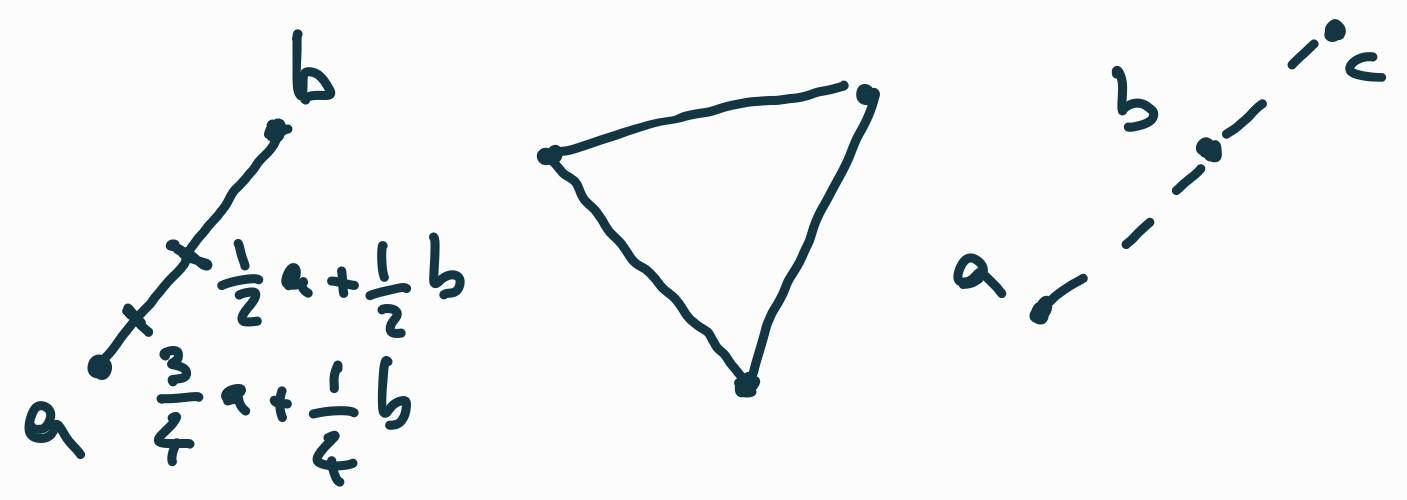
\includegraphics[width=0.5\textwidth]{tempimages/ConvexExamples.jpg}
\end{figure}

\begin{remark}
	In terms of the convex space, all the mixtures between two ensembles correspond to the segment between them; all the mixtures between three ensembles correspond to the triangle formed by the three elements and so on. An ensemble $\ens[a]$ is a component of a different ensemble $\ens[b]$ if the segment connecting $\ens[a]$ and $\ens[b]$ can be extended past $\ens[b]$. If two elements are not a component of each other, then they are the extreme points of the line that connects the two. That is, the segment cannot be extended.
\end{remark}

\begin{figure}[H]
	\centering
	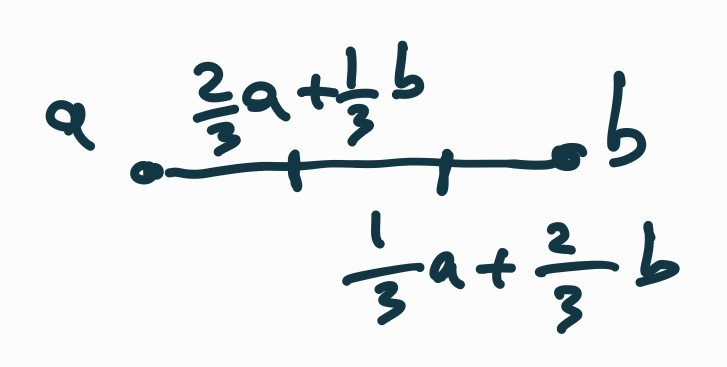
\includegraphics[width=0.4\textwidth]{tempimages/ComponentNotOrder.jpg}
\end{figure}

\begin{remark}
	Note that two ensembles can be components of each other. Consider $\frac{2}{3} \ens[a] + \frac{1}{3} \ens[b]$ and $\frac{1}{3} \ens[a] + \frac{2}{3} \ens[b]$. We can write $\frac{2}{3} \ens[a] + \frac{1}{3} \ens[b] = \frac{1}{2}\left(\frac{1}{3} \ens[a] + \frac{2}{3} \ens[b]\right) + \frac{1}{2} \ens[a]$ and $\frac{1}{3} \ens[a] + \frac{2}{3} \ens[b] = \frac{1}{2}\left(\frac{2}{3} \ens[a] + \frac{1}{3} \ens[b]\right) + \frac{1}{2} \ens[b]$ (they are both midpoints along each other). Therefore a component is not necessarily ``smaller'' or ``better defined'' than the mixture. Mathematically, ``being a component of'' is not a partial order. It is reflexive and transitive, but it is not antisymmetric. In practical terms, we need something else to tell us whether we are, for example, taking a limit with components that become ``smaller and smaller.''
\end{remark}
\end{mathSection}

We can also characterize some ensembles based on what other ensembles they can admit as components. An extreme point is an ensemble that has only itself as a component. For example, a pure state will be an extreme point as it cannot be expressed as a mixture of any other states. Conversely, an internal point is an ensemble that admits any other ensemble as a component. For example, in a finite discrete classical space, the uniform distribution over all cases can be seen the mixture of any other distribution with something else. A boundary point is an ensemble that is neither an extreme or an internal point. The figure helps visualize the properties.

\begin{mathSection}
\begin{defn}
	Let $\Ens$ be an ensemble space. An \textbf{extreme point} $\ens \in \Ens$ is an ensemble that has no component distinct from itself. That is, there is no $\ens[a] \in \Ens\setminus\{ \ens \}$ such that $\ens = p \ens[a] + \bar{p} \ens[b]$ for some $p \in (0,1]$ and $\ens[b] \in \Ens$. An \textbf{internal point} $\ens \in \Ens$ is an ensemble for which every ensemble is a component. That is, for every $\ens[a] \in \Ens$ there is always $\ens[b] \in \Ens$ and $p(0,1]$ such that $\ens = p \ens[a] + \bar{p} \ens[b]$. A \textbf{boundary point} is any ensemble that is not an internal point.
\end{defn}

\begin{remark}
	The notion of internal point parallel \href{https://en.wikipedia.org/wiki/Algebraic_interior}{the similar notion} in topological vector spaces.
\end{remark}

\begin{figure}[H]
	\centering
	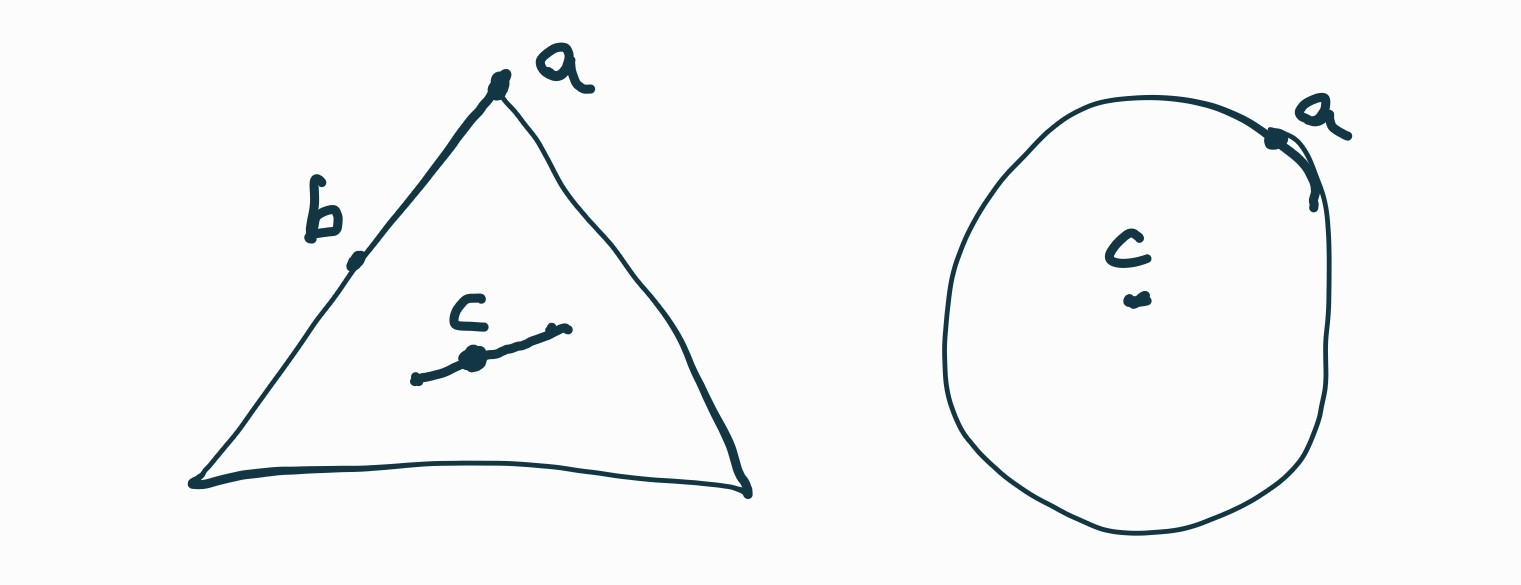
\includegraphics[width=0.8\textwidth]{tempimages/InteriorExteriorPoints.jpg}
	\caption{The ensemble $\ens[a]$ is an extreme point in both spaces. $\ens[b]$ is a boundary point, but is not an extreme point (it is the mixture of the vertices on the same side). $\ens[c]$ is an internal point.}
\end{figure}

\begin{prop}
	The set of all internal points $I_{\Ens}$ is a convex set.
\end{prop}
\begin{proof}
Let $\ens_1, \ens_2 \in I_{\Ens}$ be two internal points of $\Ens$. Since $\ens_1$ and $\ens_2$ are internal points, given any $\ens[a] \in \Ens$ we can find $\ens[b]_1, \ens[b]_2 \in \Ens$ such that 
\begin{equation}
	\begin{aligned}
	\ens_1 & =p_1 \ens[a]+\bar{p}_1 \ens[b]_1 \\
	\ens_2 & =p_2 \ens[a]+\bar{p}_2 \ens[b]_2
	\end{aligned}
\end{equation}
for some $p_1, p_2 \in [0,1]$. Now let $p \in [0,1]$ and $\ens = p \ens_1+\bar{p} \ens_2$. We have:
\begin{equation}
\begin{aligned}
	\ens = p \ens_1+\bar{p} \ens_2 &= p(p_1 \ens[a]+\bar{p}_1 \ens[b]_1) + \bar{p} (p_2 \ens[a]+\bar{p}_2 \ens[b]_2)\\
	&=\left(p p_1+\bar{p} p_2\right) \ens[a]+\left(p \bar{p}_{1} \ens[b]_1+\bar{p} \bar{p}_{2} \ens[b]_2\right) \\
	&=\lambda \ens[a] + \bar{\lambda} \left(\frac{p \bar{p}_{1}}{\bar{\lambda}} \ens[b]_1+\frac{\bar{p} \bar{p}_{2}}{\bar{\lambda}} \ens[b]_2\right) = \lambda \ens[a] + \bar{\lambda} \ens[b] \\
\end{aligned}
\end{equation}
where $\lambda = p p_1+\bar{p} p_2$ and $\ens[b] = \frac{p \bar{p}_{1}}{\bar{\lambda}} \ens[b]_1+\frac{\bar{p} \bar{p}_{2}}{\bar{\lambda}} \ens[b]_2$. Therefore, given any $\ens[a] \in \Ens$, we can find a $\ens[b] \in \Ens$ such that $\ens = \lambda \ens[a] + \bar{\lambda} \ens[b]$ for some $\lambda \in [0,1]$. This means the convex combination of internal points is an internal point, and $I_{\varepsilon}$ is a convex set.
\end{proof}

\begin{remark}
	It is an open question whether this result generalizes to infinite mixtures. That is, whether the infinite mixture of internal points is still an internal point.
\end{remark}
\end{mathSection}

For topological vector spaces, the algebraic interior and the topological interior are related. For example, if $A$ is a convex subset of a TVS with non-empty topological interior, then the algebraic and topological interior coincide. It is an open question how many of these results hold for topological convex space as well. As an example, we would like to prove the following.

\begin{conj}
	Let $\Ens$ be an ensemble space with a $T_1$ topology. The set of boundary points $B_{\Ens}$ is a closed set and therefore $I_{\Ens}$ is an open set.
\end{conj}
\begin{remark}
	One may be able to show that the limit of a sequence of boundary points cannot be an interior point.
\end{remark}

We now define the notions of separateness: two ensembles are separate, noted $\ens[a] \separate \ens[b]$ if they do not have a common component. That is, they are not a mixture of a common ensemble. In classical ensemble spaces, this is equivalent to probability measures with disjoint support, which is the extension of the concept. Separateness is a useful concept to characterize the relationship between ensembles as it has some useful property. Most of all, it is an irreflexive symmetric relation: everything is not separate from itself and if $\ens[a] \separate \ens[b]$, then $\ens[b] \separate \ens[a]$.\footnote{Note that orthogonality in inner product vector spaces is also an irreflexive symmetric relationship.}

\begin{mathSection}
\begin{defn}
	Let $\Ens$ be an ensemble space and $\ens[a], \ens[b] \in \Ens$. We say that they \textbf{have a common component} if we can find $\ens[c] \in \Ens$, the common component, such that $\ens[a] = p_1 \ens[c] + \bar{p}_1 \ens_1$ and $\ens[b] = p_2 \ens[c] + \bar{p}_2 \ens_2$ for some $\ens_1, \ens_2 \in \Ens$ and $p_1, p_2 \in (0,1]$. Otherwise, we say they \textbf{have no common component}, or are \textbf{separate}, noted $\ens[a] \separate \ens[b]$. Two ensembles have a common component in $A \subseteq \Ens$ if the common component can be found in $A$, and are separate in $A$ if there is none. Two sets of ensembles $A, B \subseteq \Ens$ are separate if all the elements of one are separate from all the elements of the other. That is, $A \separate B$ if $\ens[a] \separate \ens[b]$ for all $\ens[a] \in A$ and $\ens[b] \in B$.
\end{defn}

\begin{figure}[H]
	\centering
	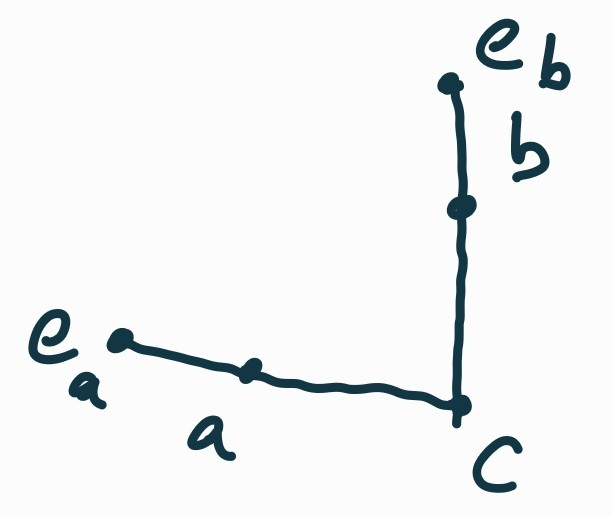
\includegraphics[width=0.3\textwidth]{tempimages/CommonComponent.jpg}
\end{figure}

\begin{remark}
	If two ensembles $\ens[a]$ and $\ens[b]$ have a common component $\ens[c]$, then the ensemble space contains a triangle where $\ens[c]$ is a vertex and $\ens[a]$ and $\ens[b]$ are points on the sides that connect to $\ens[c]$.
\end{remark}

\begin{coro}
	The previous definitions obey the following:
	\begin{enumerate}
		\item every ensemble is a component of itself
		\item if $\ens[a]$ is a component of $\ens[b]$, then $\ens[a]$ and $\ens[b]$ have a common component and therefore they are not separate
		\item separateness is an irreflexive symmetric relation
		\item an ensemble is an extreme point if and only if it is separate from all other ensembles
		\item an ensemble is an internal point if and only if it is not separate from any ensemble
	\end{enumerate}
\end{coro}

\begin{proof}
	1. Since by idempotence $\ens = p \ens + \bar{p} \ens$ for any $p$, then every ensemble is a mixture of itself, and therefore it is a component of itself.
	
	2. By idempotence, we can write $\ens[a] = p_1 \ens[a] + \bar{p}_1 \ens[a]$ for some $p_1 \in (0,1]$. Since $\ens[a]$ is a component of $\ens[b]$, we can write $\ens[b] = p_2 \ens[a] + \bar{p}_2 \ens[e]_2$ for some $p_2 \in (0, 1]$ and $\ens[c] \in \Ens$. Therefore $\ens[a]$ and $\ens[b]$ have $\ens[a]$ as a common component.
	
	3. Since every ensemble is a component of itself, every ensemble has a common component with itself and therefore is not separate from itself. This proves that separateness is irreflexive. The definition of common component is symmetric and therefore so is separateness.
	
	4. An extreme point has only itself as a component, therefore it can have a common component only with itself.
	
	5. Every ensemble is a component of an internal point, therefore every ensemble is not separate from an internal point
\end{proof}
\end{mathSection}

One key property of separateness is its relationship with mixtures. If an ensemble is separate from a mixture of two elements, it is separate from both elements and all their mixtures. Note that the converse, as we show in the example below, is not true in general. It is true in classical ensembles spaces (i.e. a probability distribution has disjoint support with other two distributions if and only if it has disjoint support from any convex combination) but not in quantum mechanics. This is another reason why this property is important to characterize ensemble spaces in general.

\begin{mathSection}
\begin{prop}[Separateness extends to all mixtures]\label{pm_es_separateExtendsMixtures}
	Let $\ens,\ens_1,\ens_2 \in \Ens$. If $\ens$ has no common component with a mixture of $\ens_1$ and $\ens_2$ then it has no common component with any mixture of $\ens_1$ and $\ens_2$ and with either $\ens_1$ or $\ens_2$. That is, if $\ens \separate p \ens_1 + \bar{p} \ens_2$ for some $p \in (0, 1)$ then $\ens \separate p \ens_1 + \bar{p} \ens_2$ for all $p \in [0, 1]$.
\end{prop}

\begin{figure}[H]
	\centering
	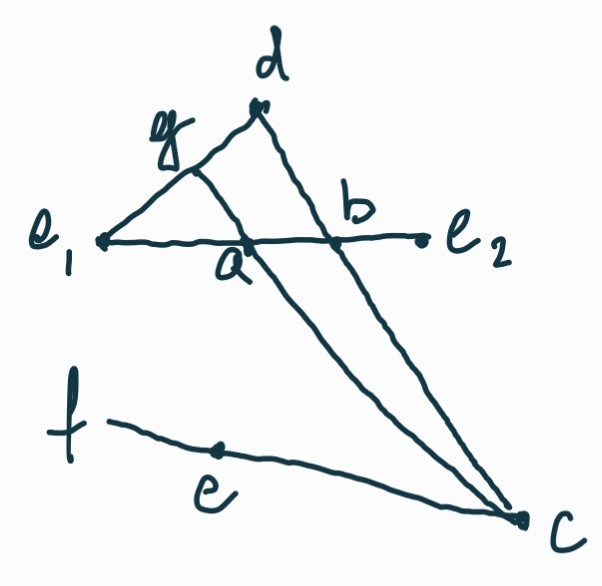
\includegraphics[width=0.3\textwidth]{tempimages/DistinctAndMixture.jpg}
\end{figure}

\begin{proof}
	Let $\ens \separate \ens[a] = p \ens_1 + \bar{p} \ens_2$ for some $p \in (0, 1)$. Let $\ens[b] = \alpha \ens_1 + \bar{\alpha} \ens_2$ with $0 \leq \alpha < p$. Suppose $\ens[b]$ is not separate from $\ens$. Then we can find $\ens[c] \in \Ens$ such that $\ens[b] = \beta \ens[c] + \bar{\beta} \ens[d]$ and $\ens = \gamma \ens[c] + \bar{\gamma} \ens[f]$ for some $\ens[d], \ens[f] \in \Ens$ and $\beta, \gamma \in (0, 1)$.
	
	Setting $\epsilon = \frac{p - \alpha}{\bar{\alpha}}$ and $\lambda = \bar{\epsilon} \beta$ we have:
	\begin{align*}
		\ens[a] &= p \ens_1 + \bar{p} \ens_2 = \left(p - \frac{\bar{p}}{\bar{\alpha}} \alpha \right) \ens_1 + \frac{\bar{p}}{\bar{\alpha}} \alpha \ens_1 + \frac{\bar{p}}{\bar{\alpha}} \bar{\alpha}\ens_2 \\
		&= \left(\frac{p\bar{\alpha} - \bar{p}\alpha}{\bar{\alpha}} \right) \ens_1 + \frac{\bar{p}}{\bar{\alpha}} (\alpha \ens_1 + \bar{\alpha} \ens_2) = \left(\frac{p - p\alpha - \alpha + p \alpha}{\bar{\alpha}} \right) \ens_1 + \frac{1 - p + \alpha - \alpha}{\bar{\alpha}} (\alpha \ens_1 + \bar{\alpha} \ens_2) \\
		&= \frac{p - \alpha}{\bar{\alpha}}  \ens_1 + \left( 1 - \frac{p - \alpha}{\bar{\alpha}}\right) (\alpha \ens_1 + \bar{\alpha} \ens_2) = \epsilon \ens_1 + \bar{\epsilon} (\alpha \ens_1 + \bar{\alpha} \ens_2) = \epsilon \ens_1 + \bar{\epsilon} \ens[b] \\
		&= \epsilon \ens_1 + \bar{\epsilon} ( \beta \ens[c] + \bar{\beta} \ens[d] ) = \bar{\epsilon} \beta \ens[c] + \epsilon \ens_1 + \bar{\epsilon} \bar{\beta} \ens[d] = \lambda \ens[c] + \bar{\lambda} \ens[g]
	\end{align*}
	where $\ens[g] = \frac{1}{\bar{\lambda}}\left( \epsilon \ens_1 + \bar{\epsilon} \bar{\beta} \ens[d] \right)$. This means $\ens[a]$ and $\ens$ have a common component, which is a contradiction. Therefore $\ens \separate \alpha \ens_1 + \bar{\alpha} \ens_2$ for all $\alpha \in [0, p]$.
	
	We can repeat the argument switching $\ens_1$ with $\ens_2$ and find $\ens \separate \alpha \ens_1 + \bar{\alpha} \ens_2$ for all $\alpha \in [0, 1]$.
\end{proof}

\begin{figure}[H]
	\centering
	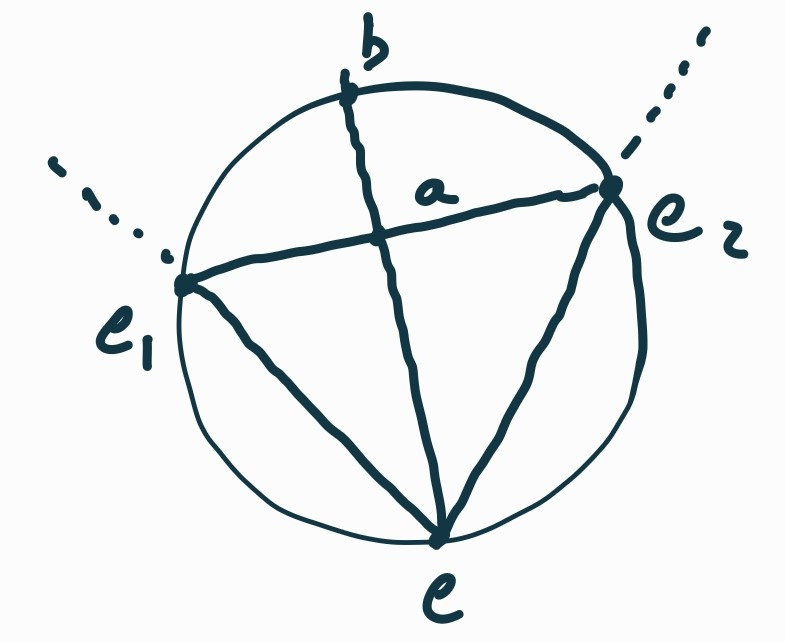
\includegraphics[width=0.3\textwidth]{tempimages/MixturesDoNotPreserveSeparateness.jpg}
\end{figure}

\begin{remark}
	Note that the property does not work the other way around, in the sense that $\ens \separate \ens_1$ and $\ens \separate \ens_2$ does not imply $\ens \separate \alpha \ens_1 + \bar{\alpha} \ens_2$ for all $\alpha \in [0, 1]$. We can find a counterexample in quantum mechanics. Suppose that $\ens$, $\ens_1$ and $\ens_2$ are three pure states within the same two-dimensional subspace. These will be points on the surface of a Bloch ball, which will identify a circle. Since they are pure states, they will be all separate. However, if we take a mixture $\ens[a]$ of $\ens_1$ and $\ens_2$, this can also be written as a mixture of $\ens$ and some $\ens[b]$. Since $\ens$ is a component of $\ens[a]$, they are not separate.
\end{remark}
\end{mathSection}

\subsection{Convex subsets and convex hull}

In many cases, we will need to discuss the sets that contain all their possible mixtures. One typically distinguish two cases. A set is convex if it allows all possible finite mixtures. This may be too restrictive as it may not include all possible infinite mixtures. A set is closed and convex if it includes all finite mixtures and their topological limits. Given that infinite mixtures are the topological limit of finite mixtures, a closed convex set contains all infinite mixtures. However, not all topological limits can be expressed as infinite mixture. For example, on the real line $1$ can be seen as a limit of points within the open interval $(0,1)$, but not as infinite convex combination. Therefore we add the notions of $\sigma$-convex set that is closed under infinite mixtures.\footnote{The mathematical properties of $\sigma$-convex sets is yet to be explored.}

\begin{mathSection}
\begin{defn}
	Let $\Ens$ be an ensemble space. We say $A \subseteq \Ens$ is \textbf{convex} if it closed under finite mixtures (i.e. $\ens[a],\ens[b] \in A$ implies $p\ens[a] + \bar{p} \ens[b] \in A$), \textbf{$\sigma$-convex} if it is closed under infinite mixtures (i.e. $\ens[a]_i \in A$ implies $\sum_i p_i \ens[a]_i \in A$ for all converging infinite mixtures) and \textbf{closed and convex} if it is both convex and topologically closed.
\end{defn}

\begin{coro}
	A closed and convex set is $\sigma$-convex. A $\sigma$-convex set is convex.
\end{coro}
\end{mathSection}

Given a set of ensembles $A$, we can ask for all ensembles that can be constructed from $A$. The hull of $A$ is the set of all finite mixtures of $A$, the $\sigma$-hull of $A$ is the set of all infinite mixtures of $A$ and the closed hull of $A$ is the set of all the topological limits of finite mixtures of $A$. Notably, the closed hull of $A$ is equivalent to the topological closure of the hull of $A$.

\begin{mathSection}
\begin{defn}
	Let $A \subseteq \Ens$ be a subset of an ensemble space. The \textbf{convex hull} of $A$, noted $\hull(A)$ is the set of all finite mixtures of elements contained in $A$ (i.e. it is the smallest convex set that contains $A$). The \textbf{$\sigma$-hull} of $A$, noted $\shull(A)$ is the set of all infinite mixtures of elements contained in $A$ (i.e. it is the smallest $\sigma$-convex set that contains $A$). The \textbf{closed hull} of $A$, noted $\chull(A)$ is the smallest closed convex set that contains $A$. 
\end{defn}

\begin{remark}
	Note that, given a set $A$, not all elements of $\chull(A)$ can be understood as infinite mixtures. That is, we can have $\shull(A) \subset \chull(A)$. Let $\Ens$ bet the line segment $[0,1]$ and consider the set $A=\left\{\frac{1}{2^i}\right\}_{i=0}^{\infty}$. Every point in $(0,1]$ can be expressed as a finite mixture of two elements of $A$. For example, $1$ and any number smaller than the target number. However, zero cannot be expressed as a convex combination of positive numbers, and therefore it is not an infinite mixture of $A$. However, zero is the limit of the sequence, and therefore it will be in the topological closure of $A$.
\end{remark}

\begin{coro}
	Given $A \subseteq \Ens$, $\hull(A) \subseteq \shull(A) \subset \chull(A)$.
\end{coro}

\begin{proof}
	All finite mixtures are also infinite mixtures with $p_i = 0$ for all $i > n$ for some $n$. Therefore $\hull(A) \subseteq \shull(A)$. All infinite mixtures are topological limits of finite mixtures. Therefore $\shull(A) \subseteq \chull(A)$. 
\end{proof}

\begin{coro}\label{pm_es_hullProp}
	All three hull operators are closures. That is, for $\hull$ we have
	\begin{enumerate}
		\item $A \subseteq \hull(A)$
		\item $A \subseteq B \implies \hull(A) \subseteq \hull(B)$
		\item $\hull(\hull(A)) = \hull(A)$
	\end{enumerate}
	and similarly for $\shull$ and $\chull$.
\end{coro}

\begin{proof}
	1. Every element of $A$ is trivially a mixture of elements of $A$. Therefore $A \subseteq \hull(A)$. Since $\hull(A) \subseteq \shull(A) \subset \chull(A)$, $A \subseteq \shull(A)$ and $A \subseteq \chull(A)$ as well. 
	
	2. Let $\ens \in \hull(A)$. Then it is a finite mixture of some elements of $A$. Since $A \subseteq B$, then $\ens$ is also the finite mixture of some elements of $B$ and therefore $\ens \in \hull(B)$. The same logic applies to the $\sigma$-hull and closed hull replacing finite mixture with the appropriate operation.
	
	3. Since $\hull(\hull(A))$ is the smallest convex subset that contains $\hull(A)$, and since $\hull(A)$ is a convex subset, then $\hull(\hull(A))$ must be $\hull(A)$ since no smaller set can contain all elements of $\hull(A)$. The same logic applies to the $\sigma$-hull and closed hull.
\end{proof}

\begin{coro}
	A subset $A \subseteq \Ens$ is respectively convex/$\sigma$-convex/closed convex if and only if it is its own convex hull/$\sigma$-hull/closed hull.
\end{coro}

\begin{proof}
	Let $A \subseteq \Ens$ be a convex subset. By \ref{pm_es_hullProp} we have $A \subseteq \hull(A)$. By definition of convex set, we have $\hull(A) \subseteq A$. Therefore $A = \hull(A)$. Conversely, let $A \subseteq \Ens$ be a set of ensembles not necessarily convex and let $A=\hull(A)$. By definition, $\hull(A)$ is closed under finite mixture and is therefore a convex subset. The same logic applies to the $\sigma$-convex and closed convex with the respective hull.
\end{proof}

\begin{defn}
	We note $\mathfrak{co}_{\Ens}$ the set of all convex subsets of $\Ens$, $\mathfrak{sco}_{\Ens}$ the set of all $\sigma$-convex subsets of $\Ens$ and $\mathfrak{cco}_{\Ens}$ the set of all closed convex subsets of $\Ens$.
\end{defn}

\begin{prop}
	The sets $\mathfrak{co}_{\Ens}$, $\mathfrak{sco}_{\Ens}$ and $\mathfrak{cco}_{\Ens}$, as posets ordered by inclusion, are topped $\bigcap$-structure and therefore complete lattices.
\end{prop}

\begin{proof}
	Theorem 7.3 in Davey, Priestley Introduction to Lattice and Order states that, given a closure operator, the set of all closures, ordered by inclusion, is a topped $\bigcap$-structure and therefore complete lattices. Since $\mathfrak{co}_{\Ens}$, $\mathfrak{sco}_{\Ens}$ and $\mathfrak{cco}_{\Ens}$ are closures, the theorem applies.
\end{proof}

\begin{remark}
It may be interesting to see whether the hulls are continuous from above and below. That is, whether  $\hull(\lim\limits_{i \to \infty} A_i) = \lim\limits_{i \to \infty} \hull(A_i)$ for decreasing or increasing sequences.

All hulls should be continuous from above as the arbitrary union remains within the corresponding lattice. The closed hull, however, should not be necessarily continuous from below. That is, it is not necessarily true that $\hull(\lim\limits_{i \to \infty} A_i) = \lim\limits_{i \to \infty} \hull(A_i)$ for any increasing sequence $A_i \subseteq \Ens$. The limit from below, in fact, would correspond to the infinite union of closed sets, which is not necessarily a closed set. Therefore if we take the closure after the limit, we are going to include the infinite convex combinations that require, for example, an element from each of the $A_i$.
\end{remark}


\begin{prop}
	The topological closure of the hull is a convex set and, therefore, the closed hull.
\end{prop}

\begin{proof}
	Let $A$ be a convex set and $\bar{A}$ its topological closure. Let $\ens[a]_i, \ens[b]_i \in A$ be two sequences that converge to $\ens[a], \ens[b] \in \Ens$ respectively. We have $\ens[a], \ens[b] \in \bar{A}$ since they are topological limits. Consider $\ens_i = p \ens[a]_i + \bar{p} \ens[b]_i$. Since mixing is continuous, we have:
	\begin{equation}
		\begin{aligned}
			\ens &= p \ens[a] + \bar{p} \ens[b] = p \lim\limits_{i \to \infty} \ens[a]_i + \bar{p} \lim\limits_{i \to \infty} \ens[b]_i = \lim\limits_{i \to \infty} p \ens[a]_i + \bar{p} \ens[b]_i = \lim\limits_{i \to \infty} \ens_i.
		\end{aligned}
	\end{equation}
	But $\ens_i$ are finite mixtures of elements of $A$, and therefore $\ens_i \in A$ is a sequence of elements of $A$. The sequence converges, $\ens$ is the limit of a sequence of elements of $A$ and therefore $\ens \in \bar{A}$. That is, the topological closure of a convex set is also a convex set. But this means that $\bar{A}$ is a closed convex set. Since any closed convex set that contains $A$ will also need to contain $\bar{A}$, $\bar{A}$ is the closed hull of $A$.

	Let $A \subset \Ens$ be a subset not necessarily convex, $\hull(A)$ will convex. Therefore its topological closure will be the closed hull of $A$.
\end{proof}

\end{mathSection}

Something that still need to be explored is the relationship between the algebraic interior and topological interior. For example, is every interior point an internal point? Given a set of internal points of $\Ens$, is the $\sigma$-hull a set of internal points? It would seem so, as convex combinations cannot bring us to the boundary of a set. Given $A$, if $\ens \in \chull(A)$ is an internal point with respect to $\chull(A)$, does it mean that $\ens \in \shull(A)$?



\section{Axiom of entropy}

In this section we will see how characterizing the variability of the elements within an ensemble leads to the standard notion of entropy. The entropy will have to satisfy few basic properties justified by the notion of variability which will be enough to recover the usual Shannon formula. It will also provide us with another basic notion to compare ensembles: two ensembles are mutually exclusive, or orthogonal, if they have no elements in common, which means the entropy will maximally increase during mixing. The interaction between orthogonality and separateness is enough to understand the differences between classical and quantum systems.

We saw that our basic notion of state is that of an ensemble. Since an ensemble represents all possible preparations of equivalent systems prepared according to the same procedure, we want to characterize how much those instances are different from each other. To be truly general, we want to be able to make this characterization without assumption of what the individual instances are.\footnote{There a sense that the instances cannot ever be fully characterized scientifically precisely because they are irrepeatable. Suppose, in fact, that we want to construct a measurement device to characterize each instance. Each possible output of the measurement device will need to be checked and calibrated: we will need to make sure that when a particular values is outputted is because the corresponding input was presented. To be able to do, we need a way to reliably prepare all possible inputs to the precision we are tuning the device. Therefore, we will be able to distinguish instances only insofar we are able to prepare finely tuned ensembles of those instances. Effectively, we are only able to distinguish between the ensembles we are able to prepare. More philosophical work would be welcome on this topic.} First of all, the variability should be an experimentally well-defined quantity, and it should therefore be a continuous function in the natural topology. It should also be compatible with statistical mixing. Intuitively, the variability cannot decrease during mixing which makes the entropy a strictly concave function. Variability will have a maximal increase when mixing ensembles that are mutually exclusive: no instance of one can be confused with an instance of the other. In that case, the increase of the variability is fully characterized by the mixing coefficients. We say that to mutually exclusive ensembles are orthogonal, as this property will correspond mathematically to orthogonality in the space of distributions. Lastly, if one ensemble has no instances in common with other two, then it has no instance in common with any mixture of the two.

Thinking of ensembles and the variability of their instances, then, makes it clear what entropy is and why does it have these properties. We are not concerned, at this point, what the source of the variability is. We just know that it is something that we need to characterize.

\begin{mathSection}
\begin{axiom}[Axiom of entropy]
	Every element of the ensemble is associated with an \textbf{entropy} which quantifies the variability of the preparations of the ensemble. Formally, an ensemble space $\Ens$ is equipped with a function $S : \Ens \to \mathbb{R}$, defined up to a positive multiplicative constant representing the unit numerical value. The entropy has the following properties:
	\begin{itemize}
		\item \textbf{Continuity}\footnote{Currently, we are imposing that the entropy is continuous. There may be a chance that this requirement is redundant, as strict concavity and the upper variability bound may already impose this. We have found proofs that show that real valued convex/concave functions of real values are continuous. These proofs fail at the extreme points, but the upper variability bound may fix this. Another open question is whether differentiability is also an independent requirement.}
		\item \textbf{Strict concavity}: $S(p\ens[a] + \bar{p} \ens[b]) \geq p S(\ens[a]) + \bar{p} S(\ens[b])$ with the equality holding if and only if $\ens[a] = \ens[b]$
		\item \textbf{Upper variability bound}: there exists a universal function $I(p_1, p_2)$ (i.e. the same for all ensemble spaces) such that $S(p\ens[a] + \bar{p} \ens[b]) \leq I(p, \bar{p}) + p S(\ens[a]) + \bar{p} S(\ens[b])$; if the equality holds, $\ens[a]$ and $\ens[b]$ are \textbf{mutually exclusive} or \textbf{orthogonal}, noted $\ens[a] \ortho \ens[b]$
		\item \textbf{Mixtures preserve orthogonality}:\footnote{It is unclear whether ``mixtures preserve orthogonality'' is an independent axiom. Intuitively, the following argument tells us that it is. Take the 2 dimensional simplex (i.e. a triangle) that represents a classical discrete probability space over three elements. Take the standard entropy, which will satisfy ``mixtures preserve orthogonality''. This is because the middle point has entropy $\log 3$. We can imagine redefining the entropy so that it is a little bit lower in the center but it is unchanged on the sides. However, one needs to provide an actual example and show that it satisfies all axioms. It may also be that only one direction is an independent axiom. That is, that orthogonality with the components implies orthogonality with the mixtures. This is what does not hold for separateness.} $\ens[a] \ortho \ens[b]$ and $\ens[a] \ortho \ens[c]$ if and only if $\ens[a] \ortho p \ens[b] + \bar{p} \ens[c]$ for any $p \in (0,1)$
	\end{itemize}
\end{axiom}

\begin{justification}
	The entropy quantifies the variability of the instances within an ensemble. Since the ensemble represents a collection of preparations of equivalent systems, and since each instance will in general be potentially different, it is legitimate to ask how much variability there is among the different instances. We are assuming that the entropy is a quantity (i.e. a linearly ordered property), meaning that it is always meaningful to tell whether one ensemble has more variability than another. If this is the case, the later requirements of continuity and strict concavity will force the entropy to be a real valued quantity. This is because the variability will change under statistical mixtures, and since statistical mixtures are performed with real valued coefficients, the variability will have to be a real valued quantity. Whether it is conceptually possible to have a characterization of variability that is not linearly ordered but still have a meaningful connection with statistical mixing is an open question, therefore we are not able to fully justify entropy's linear ordering at this time. Therefore the linear ordering of the entropy should be considered an assumption. Provided that assumption, we are justified to assume the existence of a real valued function that returns the entropy, a measure of variability of the ensemble.
	
	Since the entropy is a real valued quantity, it will have a corresponding unit. This unit is independent from all other units, and therefore the overall structure of the ensemble space must be independent of this choice. Mathematically, the physical dimension of the unit is not captured, just its numeric value. A change of unit may change the numeric value by a multiplicative constant. Since variability is an ordered quantity, we want the change of units to respect the ordering and therefore it should be a positive multiplicative constant. This justifies that the entropy function is defined up to a positive multiplicative constant.
	
	Note that the additivity of the entropy over independent systems fixes the absolute scale. If $S_{AB} = S_A + S_B$, in fact, one can't rescale all three terms by an additive factor and preserve the relationship.
	
	The variability, in the end, will have physical consequences, and it will therefore be measurable, thus experimentally verifiable: it will have to be a topologically continuous function. Moreover, small changes in the ensemble should produce small changes in the variability, which justifies analytical continuity. We are therefore justified to assume continuity of the entropy.
	
	Suppose we have two ensembles and we perform a statistical mixture. There are going to be three sources of variability: the two ensembles and the random choice at every instance. The total contribution from the original ensembles will be the average variability of the original ensembles. This is increased by the variability introduced by the random choice, which is always a positive contribution. Therefore the final variability cannot be less than the average of the original ensembles. That is, $S(p\ens[a] + \bar{p} \ens[b]) \geq p S(\ens[a]) + \bar{p} S(\ens[b])$. If we are mixing an ensemble with itself, this is equivalent to just choosing from the original ensemble, therefore the variability will not increase. Conversely, if the variability stays the same, it means that the random choice does not increase the variability, and therefore we must be choosing between equivalent ensembles. Therefore we are justified to assume that entropy is strictly concave.
	
	On the other hand, the variability cannot increase arbitrarily during mixture. The maximum variability will be given when the two ensembles are mutually exclusive, when an instance of the first ensemble cannot be produced by the second ensemble. That is, a single instance is enough to determine whether we have the first ensemble or the second. In this case, the variability is increased by the variability of the random choice, which must depend only on the mixture coefficient, and not the nature of the ensembles themselves. That is, $S(p\ens[a] + \bar{p} \ens[b]) \leq I(p, \bar{p}) + p S(\ens[a]) + \bar{p} S(\ens[b])$ is the upper variability bound, which is saturated if and only if the $\ens[a]$ and $\ens[b]$ are mutually exclusive. The actual function $I$ is left unspecified and, as we show in proposition \ref{pm_es_entropyUnique}, it will correspond to the Shannon entropy as it is the only indicator of variability that will satisfy the axiom of entropy. This justifies the upper variability bound.
	
	Now suppose ensemble $\ens[a]$ is mutually exclusive from both $\ens[b]$ and $\ens[c]$. That is, an instance of $\ens[a]$ cannot ever be produced by either $\ens[b]$ or $\ens[c]$. Then an instance of $\ens[a]$ cannot be produced by a mixture of $\ens[b]$ and $\ens[c]$, since ultimately a mixture of $\ens[b]$ and $\ens[c]$ will return an instance of one of the two. Therefore $\ens[a]$ is mutually exclusive from any mixture of $\ens[b]$ and $\ens[c]$. The argument works in reverse as well: if an instance of $\ens[a]$ cannot be produced by a mixture of $\ens[b]$ and $\ens[c]$, then it cannot be produced by either. This justifies mixtures preserve orthogonality.
\end{justification}
\end{mathSection}

As with the other axioms, we should now verify that the axiom of entropy is satisfied by the standard cases.

\begin{mathSection}
	\begin{prop}
		Discrete classical ensemble spaces, continuous classical ensemble spaces and quantum ensemble spaces satisfy the axiom of entropy.
	\end{prop}
	
	\begin{proof}
		Let's first look at the classical continuous case. Every ensemble is represented by a distribution $\rho(x)$ with $\int_X \rho(x) d\mu=1$. The entropy is given by $S(\rho) = - \int_X \rho \log \rho d\mu$. This is a continuous function of $\rho$.
		
		\begin{figure}[H]
			\centering
			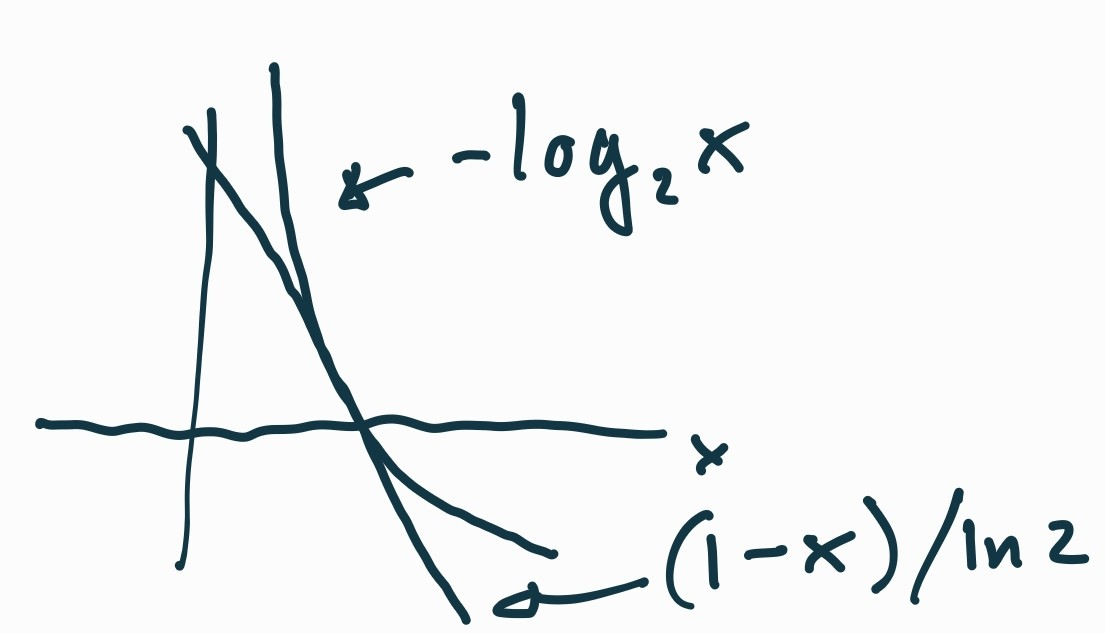
\includegraphics[width=0.5\textwidth]{tempimages/LogBound.jpg}
		\end{figure}
		
		To show strict concavity, note that $- \log x \geq \frac{1-x}{\ln 2}$ with the equality holding if and only if $x=1$. We have
		\begin{equation}
			\begin{aligned}
				S(p\rho_1 + \bar{p}\rho_2) &= - \int_X \left(p\rho_1 + \bar{p}\rho_2\right) \log \left(p\rho_1 + \bar{p}\rho_2\right) d\mu \\
				&= - \int_X p\rho_1 \log \left(p\rho_1 + \bar{p}\rho_2\right) d\mu - \int_X \bar{p}\rho_2 \log \left(p\rho_1 + \bar{p}\rho_2\right) d\mu \\
				&= - \int_X p\rho_1 \log \frac{p\rho_1 + \bar{p}\rho_2}{\rho_1} d\mu - \int_X p\rho_1 \log \rho_1 d\mu \\
				&- \int_X \bar{p}\rho_2 \log \frac{p\rho_1 + \bar{p}\rho_2}{\rho_2} d\mu - \int_X \bar{p}\rho_2 \log \rho_2 d\mu \\
				&\geq \int_X p\rho_1 \frac{1}{\ln 2} \left(1 - \frac{p\rho_1 + \bar{p}\rho_2}{\rho_1} \right)   d\mu - p \int_X \rho_1 \log \rho_1 d\mu \\
				&+ \int_X \bar{p}\rho_2 \frac{1}{\ln 2} \left(1 - \frac{p\rho_1 + \bar{p}\rho_2}{\rho_2} \right)   d\mu - \bar{p} \int_X \rho_2 \log \rho_2 d\mu \\
				&= \frac{p}{\ln 2}\left[ \int_X \rho_1 d\mu - \int_X \left(p\rho_1 + \bar{p}\rho_2\right) d\mu  \right] + p S(\rho_1) \\
				&+ \frac{\bar{p}}{\ln 2}\left[ \int_X \rho_2 d\mu - \int_X \left(p\rho_1 + \bar{p}\rho_2\right) d\mu  \right] + \bar{p} S(\rho_2) \\
				&= \frac{p}{\ln 2}\left[ 1 - 1  \right] + p S(\rho_1) + \frac{\bar{p}}{\ln 2}\left[ 1 - 1 \right] + \bar{p} S(\rho_2) \\
				&= p S(\rho_1) + \bar{p} S(\rho_2) \\
			\end{aligned}
		\end{equation}
		The equality holds if and only if $\frac{p\rho_1 + \bar{p}\rho_2}{\rho_1} = 1$ which is exactly when $\rho_1 = \rho_2$.
		
		
		\begin{figure}[H]
			\centering
			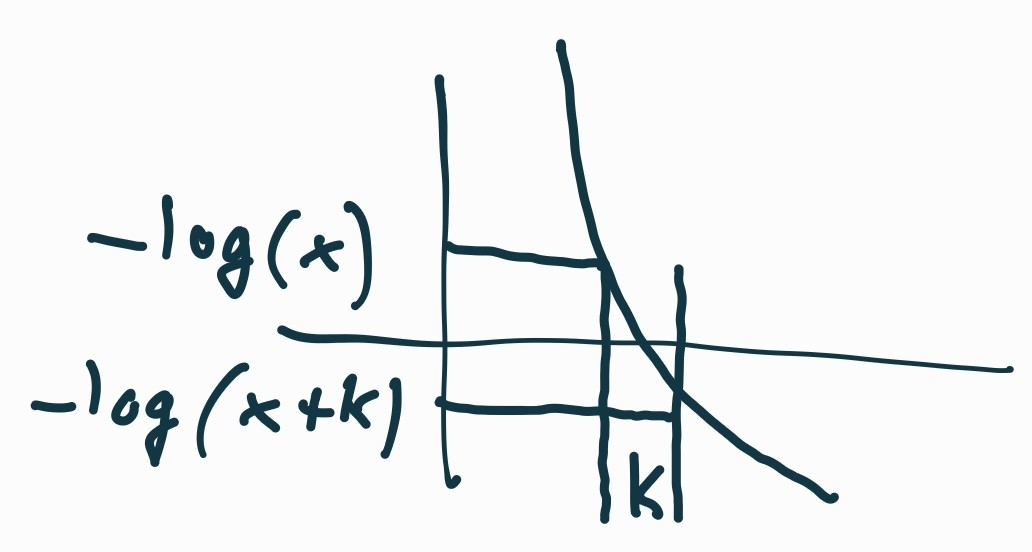
\includegraphics[width=0.5\textwidth]{tempimages/LogMonotone.jpg}
		\end{figure}
		For the upper bound, note that the logarithm is a strictly increasing function, and therefore $- \log(x + k) \leq -\log(x)$ for any $k \geq 0$, with equality holding if and only if $k=0$. We have
		\begin{equation}
			\begin{aligned}
				S(p\rho_1 + \bar{p}\rho_2) &= - \int_X \left(p\rho_1 + \bar{p}\rho_2\right) \log \left(p\rho_1 + \bar{p}\rho_2\right) d\mu \\
				&= - \int_X p\rho_1 \log \left(p\rho_1 + \bar{p}\rho_2\right) d\mu - \int_X \bar{p}\rho_2 \log \left(p\rho_1 + \bar{p}\rho_2\right) d\mu \\
				&\leq  - \int_X p\rho_1 \log p\rho_1 d\mu - \int_X \bar{p}\rho_2 \log \bar{p}\rho_2 d\mu\\
				&=  - \int_X p\rho_1 \log p d\mu - \int_X p\rho_1 \log \rho_1 d\mu - \int_X \bar{p}\rho_2 \log \bar{p} d\mu - \int_X \bar{p}\rho_2 \log \rho_2 d\mu\\
				&=  - p \log p \int_X \rho_1 d\mu - p \int_X \rho_1 \log \rho_1 d\mu - \bar{p} \log \bar{p} \int_X \rho_2 d\mu - \bar{p} \int_X \rho_2 \log \rho_2 d\mu\\
				&=  - p \log p - \bar{p} \log \bar{p} + p S(\rho_1) + \bar{p} S(\rho_2)\\
			\end{aligned}
		\end{equation}
		The equality holds if and only if $\rho_2=0$ wherever $\rho_1\neq0$ and $\rho_1=0$ wherever $\rho_2\neq0$. That is, the equality holds if and only if the two distributions have disjoint support. Therefore orthogonal distributions are exactly distributions with disjoint support.
		
		Suppose $\rho_4$ has disjoint support from $\rho_1 = p \rho_2 + \bar{p} \rho_3$, then it has disjoint support from $\rho_2$ and $\rho_3$ because the support of $\rho_1$ is the union of the supports of $\rho_2$ and $\rho_3$. Conversely, if $\rho_4$ has disjoint support from both $\rho_2$ and $\rho_3$, then $\rho_4$ has disjoint support from $\rho_1$ as well. Therefore mixtures preserve orthogonality.
		
		All these arguments are valid for discrete classical ensemble spaces, changing integrals to sums.
		
		For the quantum case, we haven't found a short proof that does not require defining the KL divergence and the entropy for a joint distribution. The result, however, is generally known and can be found, for example, in \href{https://www.cambridge.org/highereducation/books/quantum-computation-and-quantum-information/01E10196D0A682A6AEFFEA52D53BE9AE}{Nielsen-Chuang}.
	\end{proof}
\end{mathSection}


\subsection{Uniqueness of entropy of mixing coefficients}

The axiom of entropy imposes only the existence of a universal function $I(p,\bar{p})$ without specifying it's functional form. We are now going to show that the functional form is actually already fixed by the axiom: the Shannon entropy $-p \log p - \bar{p} \log \bar{p}$ is in fact the only function that is able to satisfy the axiom. The result is achieved by calculating the entropy of the same final ensemble as decomposed into a mixture in different ways. Since the final entropy should not care about how the mixture is performed, $I(p,\bar{p})$ must satisfy some properties that lead to the final results.

We note that the Shannon entropy in our framework does not represent an absolute entropy, but the maximal entropy increase during mixing. This is why we are able to keep the framework general. In fact, note that the proof does not technically know whether we are in classical or quantum ensemble space, or even in an ensemble space of a new possible theory.

\begin{mathSection}
\begin{thrm}[Uniqueness of entropy]\label{pm_es_entropyUnique}
	The entropy of the coefficients $I(p,\bar{p})$ is the Shannon entropy. That is, $I(p,\bar{p}) = - \kappa \left(p \log p + \bar{p} \log \bar{p}\right)$ where $\kappa>0$ is the arbitrary multiplicative constant for the entropy. For a mixture of arbitrarily many elements, $I(\{p_i\}) = - \kappa \sum_i p_i \log p_i$.
\end{thrm}

\begin{proof}
	Since the upper entropy bound has to be the same for all spaces, let us assume that $\Ens$ is such that it contains countably many orthogonal ensembles $\{\ens_l\}_{l=1}^{\infty}$. Since mixtures preserve orthogonality, for any convex combinations $\sum_i p_i \ens[a]_i$ of finitely many $\{\ens[a]_i\}_{i=1}^{n} \subset \{\ens_l\}_{l=1}^{\infty}$,  we have $S(\sum_i p_i \ens[a]_i ) = I_n(p_1, p_2, \dots, p_n) + \sum_i p_i S(\ens[a]_i)$ where $I_n : \mathbb{R}^n \to \mathbb{R}$ is a function of the coefficients only. Note that, given commutativity, the order of the $p_i$ does not matter and, since the coefficients can be zero, we must have $I_n(p_1, p_2, \dots, p_n) = I_{n+1}(p_1, p_2, \dots, p_n, 0)$. Therefore we can think of $I$ as a function of the coefficients and write $I(\{p_i\}_{i=1}^{n})$.
	
	We now show that $I\left(\left\{\frac{1}{n}\right\}_{i=1}^{n}\right) = \kappa \log n$ with $\kappa > 0$. That is, the maximum increase of entropy for a uniform distribution is proportional to the logarithm of the number of cases. Pick two positive integers $n, m \in \mathbb{Z}^+$. Pick $nm$ elements $\ens[a]_{jk} \in \{e_l\}_{l=1}^{\infty}$ where $1\leq j \leq n$ and $1 \leq  k \leq m$. We have:
	\begin{equation}
		\begin{aligned}
			S\left(\sum_{j=1}^{n}\sum_{k=1}^{m} \frac{1}{n}\frac{1}{m} \ens[a]_{jk}\right) &= I\left(\left\{ \frac{1}{n}\frac{1}{m}\right\}_{i=1}^{nm}\right) + \sum_{j=1}^{n}\sum_{k=1}^{m} \frac{1}{n}\frac{1}{m} S\left(\ens[a]_{jk}\right) \\
			= S\left(\sum_{j=1}^{n} \frac{1}{n} \sum_{k=1}^{m} \frac{1}{m} \ens[a]_{jk}\right)  &=I\left(\left\{ \frac{1}{n}\right\}_{i=1}^{n}\right) + \sum_{j=1}^{n} \frac{1}{n} S\left(\sum_{k=1}^{m}\frac{1}{m}\ens[a]_{jk}\right) \\
			&=I\left(\left\{ \frac{1}{n}\right\}_{i=1}^{n}\right) + \sum_{j=1}^{n} \frac{1}{n}\left(I\left(\left\{ \frac{1}{m}\right\}_{i=1}^{m}\right) +  \sum_{k=1}^{m}\frac{1}{m}S\left(\ens[a]_{jk}\right)\right) \\
			&=I\left(\left\{ \frac{1}{n}\right\}_{i=1}^{n}\right) + I\left(\left\{ \frac{1}{m}\right\}_{i=1}^{m}\right) + \sum_{j=1}^{n} \sum_{k=1}^{m}\frac{1}{n}\frac{1}{m}S\left(\ens[a]_{jk}\right).
		\end{aligned}
	\end{equation}
	Therefore
	\begin{equation}
		\begin{aligned}
			I\left(\left\{ \frac{1}{nm}\right\}_{i=1}^{nm}\right) &=I\left(\left\{ \frac{1}{n}\right\}_{i=1}^{n}\right) + I\left(\left\{ \frac{1}{m}\right\}_{i=1}^{m}\right).
		\end{aligned}
	\end{equation}
	Note that $f(n) = I\left(\left\{ \frac{1}{n}\right\}_{i=1}^{n}\right)$ is a function of $n$ only, such that $f(nm) = f(n) + f(m)$. Since $f$ is continuous, we have $f(n) = \kappa \log n$. Since the entropy is strictly concave, $\kappa$ must be positive. Therefore
	\begin{equation}
		I\left(\left\{ \frac{1}{n}\right\}_{i=1}^{n}\right) = \kappa \log n
	\end{equation}
	for some $\kappa>0$.
	
	We now show that if the coefficients $p_i$ are rationals, $I_n\left(\left\{ p_i\right\}_{i=1}^{n}\right) = - \kappa \sum_{i=1}^{n} p_i \log p_i$. Let $\{p_i\}_{i=1}^{n}$ be rational coefficients for a convex combination. We can write them as $p_i = \frac{m_i}{m}$ where $\{m_i\}, m \in \mathbb{Z}^+$ and $m$ is the least common denominator. Since $p_i$ are the coefficients of a convex combination, we must have $\sum_{i=1}^{n} m_i = m$. Since $m_i$ is a positive integer, we can write $m_i = \sum_{j=1}^{m_i} 1$. We now take $m$ orthogonal ensembles $\ens[a]_{ij}$ where $1 \leq i \leq n$ and $1 \leq j \leq m_i$. We have
	\begin{equation}
		\begin{aligned}
			S\left(\sum_{i=1}^{n}\sum_{j=1}^{m_i} \frac{1}{m} \ens[a]_{ij}\right) &= I\left(\left\{ \frac{1}{m}\right\}_{i=1}^{m}\right) + \sum_{i=1}^{n}\sum_{j=1}^{m_i} \frac{1}{m} S\left(\ens[a]_{ij}\right) \\
			&= \kappa \log m + \sum_{i=1}^{n}\sum_{j=1}^{m_i} \frac{1}{m} S\left(\ens[a]_{ij}\right) \\
		\end{aligned}
	\end{equation}
	\begin{equation}
		\begin{aligned}
			= S\left(\sum_{i=1}^{n} \frac{m_i}{m} \sum_{j=1}^{m_i} \frac{1}{m_i} \ens[a]_{ij}\right)  &=I\left(\left\{ \frac{m_i}{m}\right\}_{i=1}^{n}\right) + \sum_{i=1}^{n} \frac{m_i}{m}  S\left(\sum_{j=1}^{m_i} \frac{1}{m_i} \ens[a]_{ij}\right) \\
			&=I\left(\left\{ p_i\right\}_{i=1}^{n}\right) + \sum_{i=1}^{n} \frac{m_i}{m}\left(I\left(\left\{ \frac{1}{m_i}\right\}_{i=1}^{m_i}\right) + \sum_{j=1}^{m_i} \frac{1}{m_i} S\left(\ens[a]_{ij}\right)\right) \\
			&=I\left(\left\{ p_i\right\}_{i=1}^{n}\right) + \sum_{i=1}^{n} \frac{m_i}{m} I\left(\left\{ \frac{1}{m_i}\right\}_{i=1}^{m_i}\right) + \sum_{i=1}^{n} \frac{m_i}{m} \sum_{j=1}^{m_i} \frac{1}{m_i}S\left(\ens[a]_{ij}\right) \\
			&=I\left(\left\{ p_i\right\}_{i=1}^{n}\right) + \sum_{i=1}^{n} p_i \kappa \log m_i + \sum_{i=1}^{n}  \sum_{j=1}^{m_i} \frac{1}{m} S\left(\ens[a]_{ij}\right).
		\end{aligned}
	\end{equation}
	Therefore
	\begin{equation}
		\begin{aligned}
			\kappa \log m &= I\left(\left\{ p_i\right\}_{i=1}^{n}\right) + \sum_{i=1}^{n} p_i \kappa \log m_i \\
			I\left(\left\{ p_i\right\}_{i=1}^{n}\right) &= \kappa \log m - \sum_{i=1}^{n} p_i \kappa \log m_i = \sum_{i=1}^{n} p_i \kappa \log m - \sum_{i=1}^{n} p_i \kappa \log m_i \\
			&= - \sum_{i=1}^{n} p_i \kappa \log \frac{m_i}{m} = - \kappa \sum_{i=1}^{n} p_i \log p_i.
		\end{aligned}
	\end{equation}
	
	Lastly, let $\{p_i\}_{i=1}^{n}$ be coefficients for a convex combination, not necessarily rational. Since $I$ is continuous and $p_i$ can be approximated with rational values to an arbitrary level of precision, we will have $I\left(\left\{ p_i\right\}_{i=1}^{n}\right) = - \kappa \sum_{i=1}^{n} p_i \log p_i$. In the case of $n=2$, we have $I(p_1, p_2) = - \kappa p_1 \log p_1 - \kappa p_2 \log p_2$.	
\end{proof}

\begin{coro}
	The unit for the entropy is determined (up to the physical dimension) by the maximum of the entropy of the coefficients $I\left(\frac{1}{2}, \frac{1}{2}\right)$. If the entropy is measured in bits, then $I\left(\frac{1}{2}, \frac{1}{2}\right) = 1$.
\end{coro}

\begin{proof}
	A rescaling of the entropy will also rescale the entropy of the coefficients. Therefore setting the value of the maximum of $I$ will set the arbitrary multiplicative factor. If $I\left(\frac{1}{2}, \frac{1}{2}\right) = 1$, then $\kappa$ is equal to one and the logarithm is base two, which corresponds to the entropy measured in bits. Note that this does not fix the physical dimensions of the entropy, only the numerical value.
\end{proof}
\end{mathSection}

\subsection{Separateness and orthogonality}

Recall that orthogonality is formally defined in terms of the entropy: two ensembles are orthogonal if the entropy is maximally increase during mixture. The name was chosen because it will recover the usual notion of orthogonality for the space of distributions in both classical and quantum mechanics. Like the standard notion of orthogonality, in fact, it is irreflexive (no ensemble is orthogonal to itself) and symmetric (if $\ens[a]$ is orthogonal to $\ens[b]$, then $\ens[b]$ is orthogonal to $\ens[a]$). More over, an ensemble is not orthogonal to its own components.

% TODO for JSD: Apart from the mathematical analogy, we can see how the notion of an inner product is conceptually linked to the notion of ensemble. Consider two ensembles $\ens[a]$ and $\ens[b]$ as the two infinite collection of outputs of two preparation procedures. These are orthogonal if the ensembles are mutually exclusive: they have no instance in common. If Amanda selects one of the two preparation procedures, it may take Boris only one instance to be able to determine which preparation was selected. A full bit of information can be transferred. Now suppose $\ens[a]$ and $\ens[b]$ are distinct, but not mutually exclusive. Then the two ensembles will have some instances in common. If the instance produced by the preparation Amanda selects is one in common, then Boris cannot determine the preparation with only one measurement. The more the two ensembles are similar to each other, the less the entropy will increase during mixing, and it will not increase

Recovering the math, however, would be meaningless if we didn't also provide a stronger conceptual model. As we said, two ensembles are orthogonal if they are mutually exclusive: they have no instance in common. This means that if Amanda selects between two preparation procedures that correspond to orthogonal ensemble, Boris may only need one instance to determine which preparation was selected. A full bit of information can be transferred. This is why optimal measurements are defined across mutually exclusive, orthogonal, outcomes.

Moreover, recall that two ensembles are separate if they do not have a common component, they are not different mixture of the same ensemble. Clearly, if two ensembles do not have instances in common, they cannot be the mixture of the same ensemble. In fact, from the axioms we posed, we are able to recover that orthogonality implies separateness. One may be tempted to conclude the opposite: if two ensembles are not orthogonal, they have some instances in common and therefore we can group those common instances into a sub-ensemble of both. However, and this is the crucial problem, there is nothing that guarantee us that we can find a preparation procedure that spans only the overlap. In classical mechanics, the assumption is that we can always do it. In quantum mechanics, this does not always work and, with these concepts, it is easy to see why it should be.

Quantum states have a lower bound on the entropy. If two pure state have an overlap, the ensemble that would corresponding to that overlap would have variability lower than a pure state: it would correspond to an entropy lower than that of a pure state. That is, we cannot produce the the overlap with a reliable preparation procedure. The ensembles have instances in common but do not have an ensemble in common. This means that we have ensembles that are not mutually exclusive (i.e. not orthogonal) but do not have a common component (i.e. separate). Understanding the difference between classical and quantum mechanics lies in understanding this case.

\begin{mathSection}
\begin{prop}\label{pm_es_orthoProps}
	Orthogonality satisfies the following properties:
	\begin{enumerate}
		\item irreflexivity: $\ens[a] \northo \ens[a]$
		\item symmetry: $\ens[a] \ortho \ens[b]$ if and only if $\ens[b] \ortho \ens[a]$
		\item components are not orthogonal: if $\ens[b]$ is a component of $\ens[a]$ then $\ens[a] \northo \ens[b]$
		\item orthogonality implies separateness: if $\ens[a] \ortho \ens[b]$ then $\ens[a] \separate \ens[b]$.
	\end{enumerate}
\end{prop}

\begin{proof}
	For 1, let $\ens[a] \in \Ens$. We have $S(p\ens[a] + \bar{p}\ens[a]) = S(\ens[a]) < I(p,\bar{p}) + p S(\ens[a]) + \bar{p} S(\ens[a])$. Therefore $\ens[a]$ is not orthogonal to itself as it does not saturate the upper bound.
	
	For 2, note that the upper entropy bound is symmetric in $\ens[a]$ and $\ens[b]$.
	
	For 3, let $\ens[a] = p \ens[b] + \bar{p} \ens[c]$. Since mixtures preserve orthogonality, $\ens[b] \ortho \ens[a]$ if and only if $\ens[b] \ortho \ens[b]$ and $\ens[b] \ortho \ens[c]$. But $\ens[b]$ is not orthogonal to itself, therefore $\ens[a]$ and $\ens[b]$ are not orthogonal.
	
	For 4, we demonstrate the contrapositive: that ensembles that are not separate are not orthogonal. Let $\ens[a], \ens[b] \in \Ens$ have a common component. That is, $\ens[a] = p \ens[c] + \bar{p} \ens[d]$ and $\ens[b] = \lambda \ens[c] + \bar{\lambda} \ens[e]$. Since mixtures preserve orthogonality, $\ens[a] \ortho \ens[b]$ if and only if $\ens[a] \ortho \ens[c]$ and $\ens[a] \ortho \ens[e]$. But $\ens[c]$ is a component of $\ens[a]$, therefore they are not orthogonal. Therefore two ensembles that have a common component are not orthogonal. This means that if two ensembles are orthogonal they cannot have a common component and are therefore separate.
\end{proof}
\end{mathSection}

As we did for separateness, we extend the notion of orthogonality to sets of ensembles.

\begin{mathSection}
\begin{defn}
	Two sets of ensembles are orthogonal if all the elements of one are orthogonal to all the elements of the other. That is, $A \ortho B$ with $A, B \subseteq \Ens$ if $\ens[a] \ortho \ens[b]$ for all $\ens[a] \in A$ and $\ens[b] \in B$. 
\end{defn}

\begin{prop}
	Let $A, B \subseteq \Ens$ be two sets of ensembles such that $A \ortho B$. Then the following are true:
	\begin{enumerate}
		\item the two sets are separate: $A \separate B$
		\item their hulls are orthogonal: $\hull(A) \ortho \hull(B)$
	\end{enumerate}
\end{prop}

\begin{proof}
	For 1, by definition $\ens[a] \ortho \ens[b]$ for all $\ens[a] \in A$ and $\ens[b] \in B$. Since orthogonality implies separateness, we also have $\ens[a] \separate \ens[b]$.
	
	For 2, since mixtures preserve orthogonality, every mixture of $A$ is orthogonal to every mixture of $B$. To show that this extends to the closure, let $\ens[a]_i \in A$ and $\ens[b]_j \in B$ be two sequences of finite mixtures that converge in $A$ and $B$ respectively. Consider $f(p,\ens[a]_i, \ens[b]_j) = S(p \ens[a]_i + \bar{p} \ens[b]_j) - p S(\ens[a]_i) - \bar{p} S(\ens[b]_j)$. Since all mixtures are orthogonal, $f(p,\ens[a]_i, \ens[b]_j) = I(p,\bar{p})$. Note that $f$ is a continuous function, therefore the limits will also converge to $I(p,\bar{p})$. This means that every element in the hull of $A$ is orthogonal to every element in the hull of $B$.
\end{proof}
\end{mathSection}

TODO: Put pictures to show that orthogonal elements are on "opposite sides"

\section{Affine combinations and vector space embedding}

In this section we will see how the bounds of entropy constrain ensemble spaces to embed into vector space. Moreover, the ensemble space must be bounded along any direction. In other words, the existence of an entropy forces the convex space to rule out behaviors that would be physically pathological.

%First of all, the bounds make it possible to define a unique inverse for statistical mixture. This allows us to define affine combinations, and to show that the ensemble space is embedded into a vector space. Lastly, the bounds will force this embedding to be into a subset of a bounded set of the vector space.

\subsection{Affine combinations}

The axiom of mixture just tells us that given two ensembles and a mixing ratio, we can identify the mixture of the two ensembles. It does not guarantee the reverse. That is, given a final mixed ensembles, the mixing ratio and one component, it is not necessarily true that the second component is uniquely determined. Mathematically, the uniqueness of this type of decomposition is called the cancellative property of a convex space. This property is important as \href{https://arxiv.org/abs/1105.1270}{it can be shown} that is necessary and sufficient for the convex space to embed into a vector space.

In an ensemble space, the continuity and the strict concavity of the entropy forces the space to be cancellative. If $p \ens[a] + \bar{p} \ens = p \ens[b] + \bar{p} \ens$ for some $p \in (0,1)$, from the convex structure we can show that $p(\lambda\ens[a] + \bar{\lambda}\ens[b]) + \bar{p} \ens = p\ens[a] + \bar{p} \ens = p \ens[b] + \bar{p} \ens$ for all $p \in (0,1)$ and $\lambda \in [0,1]$. That is, if mixing $\ens$ with either $\ens[a]$ or $\ens[b]$ for some mixing coefficient $p$ yields the same result, then all non-trivial mixtures of $\ens$ with any mixture of $\ens[a]$ and $\ens[b]$ will yield the same result. But this means that the entropy cannot change as we change $\ens[a]$ to $\ens[b]$ during mixture, which can only happen if they are the same ensemble.

\begin{mathSection}
\begin{defn}
	A convex space $X$ is \textbf{cancellative} if $p \ens[a] + \bar{p} \ens = p \ens[b] + \bar{p} \ens$ for some $p \in (0,1)$ implies $\ens[a] = \ens[b]$.
\end{defn}

\begin{thrm}[Ensemble spaces are cancellative]
	Let $\Ens$ be an ensemble space. Let $\ens[a], \ens[b], \ens \in \Ens$ such that $p\ens[a] + \bar{p} \ens = p \ens[b] + \bar{p} \ens$ for some $p \in (0,1)$. Then $\ens[a] = \ens[b]$.
\end{thrm}

\begin{proof}
	Let $\ens[a], \ens[b], \ens \in \Ens$ such that $p_0\ens[a] + \bar{p}_0 \ens = p_0 \ens[b] + \bar{p}_0 \ens$ for some $p_0 \in (0,1)$.
	
	First, we show that $p\ens[a] + \bar{p} \ens = p \ens[b] + \bar{p} \ens$ for all $p \in (0,p_0]$. In that case, since $0 < \frac{p}{p_0} \leq 1$, we have
	\begin{equation}
		\begin{aligned}
			p \ens[a] + \bar{p} \ens &= \frac{p}{p_0} (p_0 \ens[a] + \bar{p}_0 \ens) + \overline{\left(\frac{p}{p_0}\right)} \ens = \frac{p}{p_0} (p_0 \ens[b] + \bar{p}_0 \ens) + \overline{\left(\frac{p}{p_0}\right)} \ens = p \ens[b] + \bar{p} \ens.
		\end{aligned}
	\end{equation}
	
	Now we show that $p\ens[a] + \bar{p} \ens = p \ens[b] + \bar{p} \ens$ for all $p \in (0,1)$. Since we want to be able to expand multiple times, we want to be able to find a $p \in (0,1)$ such that
	\begin{equation}
		p \ens[a] + p \ens[a] + (1-2p) \ens = p \ens[a] + \bar{p} (p_0 \ens[a] + \bar{p}_0 \ens)= p \ens[a] + \bar{p} p_0 \ens[a] + \bar{p} \bar{p}_0 \ens.
	\end{equation}
	The coefficient of the middle term on both sides of the equality, then, has to match. That is, we want $p = \bar{p} p_0$, which means
	\begin{equation}
		\begin{aligned}
			p&=(1-p)p_0=p_0 - p p_0 \\
			p_0 &= p + p p_0 = (1+p_0) p  \\
			p &= \frac{p_0}{1+p_0}
		\end{aligned}
	\end{equation}
	Note that since $p_0 > 0$ we have $p>0$, and since the numerator is always less than the denominator $p < 1$. We have
	\begin{equation}
		\begin{aligned}
			2p \ens[a] + \overline{2p} \ens &=  p \ens[a] + p \ens[a] + (1-2p) \ens =  p \ens[a] + \bar{p} (p_0 \ens[a] + \bar{p}_0 \ens) = p \ens[a] + \bar{p} (p_0 \ens[b] + \bar{p}_0 \ens) \\
			&= p \ens[a] + p \ens[b] + (1-2p) \ens = p \ens[b] + p \ens[a] + (1-2p) \ens = p \ens[b] + \bar{p} (p_0 \ens[a] + \bar{p}_0 \ens) \\
			&= p \ens[b] + \bar{p} (p_0 \ens[b] + \bar{p}_0 \ens) = p \ens[b] + p \ens[b] + (1-2p) \ens \\
			&= 2p \ens[b] + \overline{2p} \ens
		\end{aligned}
	\end{equation}
	The relationship, then, is valid for $p_1 = 2p$. Note that $p_1 > p_0$. In fact
	\begin{equation}
		\begin{aligned}
			p_1 &= \frac{2p_0}{1+p_0} > p_0  \\
			2 p_0 &> (1+p_0) p_0 = p_0 + p_0^2 \\
			p_0 &> p_0^2 \\
		\end{aligned}
	\end{equation}
	which is true since $p_0 \in (0,1)$. Since now the relationship holds for $p_1 = \frac{2 p_0}{1+p_0} > p_0 $, we can repeat the process again and find that it holds for $p_2 = \frac{2 p_1}{1+p_1} > p_1$ and so on. We thus have a sequence of elements between $0$ and $1$ and we need to determine what is the limit of this sequence. The only two fixed points of the expression $f(x) = \frac{2x}{1+x}$ are $0$ and $1$, with $0$ being a repelling fixed point and $1$ an attracting fixed point. Since we start with an element that is strictly between those values, the sequence will converge to $1$. Therefore, since we can always find a greater mixing coefficient for which the relationship holds, combined with the previous result, $p\ens[a] + \bar{p} \ens = p \ens[b] + \bar{p} \ens$ for all $p \in (0,1)$.
	
	Now we show that if  $p\ens[a] + \bar{p} \ens = p \ens[b] + \bar{p} \ens$ for all $p \in (0,1)$, then we also have $p(\lambda\ens[a] + \bar{\lambda}\ens[b]) + \bar{p} \ens = p\ens[a] + \bar{p} \ens = p \ens[b] + \bar{p} \ens$ for all $\lambda \in [0,1]$. We have
	\begin{equation}
		\begin{aligned}
			p(\lambda\ens[a] + \bar{\lambda}\ens[b]) + \bar{p} \ens &= \lambda(p \ens[a] + \bar{p} \ens) + \bar{\lambda}(p\ens[b] + \bar{p} \ens) = \lambda(p \ens[a] + \bar{p} \ens) + \bar{\lambda}(p\ens[a] + \bar{p} \ens) \\
			&= p\ens[a] + \bar{p} \ens = p\ens[b] + \bar{p} \ens 
		\end{aligned}
	\end{equation}
	
	Lastly, we show that $S(\lambda \ens[a] + \bar{\lambda} \ens[b]) = S(\ens[a]) = S(\ens[b])$ for all $\lambda \in [0,1]$. Using the entropy bounds, with $\lambda \in [0,1]$, we have
	\begin{equation}
		\begin{aligned}
			\lim\limits_{p \to 1} S(p(\lambda\ens[a] + \bar{\lambda}\ens[b]) + \bar{p}\ens) &\leq \lim\limits_{p \to 1} \left[ I(p,\bar{p}) + p S(\lambda\ens[a] + \bar{\lambda}\ens[b]) + \bar{p} S(\ens) \right] = S(\lambda\ens[a] + \bar{\lambda}\ens[b]) \\
			\lim\limits_{p \to 1} S(p(\lambda\ens[a] + \bar{\lambda}\ens[b]) + \bar{p}\ens) &\geq \lim\limits_{p \to 1} \left[ p S(\lambda\ens[a] + \bar{\lambda}\ens[b]) + \bar{p} S(\ens) \right] = S(\lambda\ens[a] + \bar{\lambda}\ens[b])
		\end{aligned}
	\end{equation}
	and therefore
	\begin{equation}
		\begin{aligned}		
			\lim\limits_{p \to 1} S(p(\lambda\ens[a] + \bar{\lambda}\ens[b]) + \bar{p}\ens) &= S(\lambda\ens[a] + \bar{\lambda}\ens[b]).
		\end{aligned}
	\end{equation}
	Using the above property, we also have
	\begin{equation}
		\begin{aligned}
			S(\lambda\ens[a] + \bar{\lambda}\ens[b]) &= \lim\limits_{p \to 1} S(p(\lambda\ens[a] + \bar{\lambda}\ens[b]) + \bar{p}\ens) = \lim\limits_{p \to 1} S(p \ens[a] +\bar{p} \ens) = S(\ens[a]) \\
			&= \lim\limits_{p \to 1} S(p \ens[b] +\bar{p} \ens) = S(\ens[b]) \\
		\end{aligned}
	\end{equation}
	Since $S(\lambda\ens[a] + \bar{\lambda}\ens[b]) = \lambda S(\lambda\ens[a] + \bar{\lambda}\ens[b]) + \bar{\lambda} S(\lambda\ens[a] + \bar{\lambda}\ens[b]) = \lambda S(\ens[a]) + \bar{\lambda} S(\ens[b])$, $\ens[a] = \ens[b]$ by strict concavity.
\end{proof}
\end{mathSection}

The fact that the convex space is cancellative essentially allows us to ``invert'' a convex combination, allowing affine combinations. An affine combinations is a linear combination where the coefficients sum to one, like in a convex combination, but coefficient can be negative, unlike in a convex combination. Conceptually we can ``take part of an ensemble out'' from another ensemble. The ability in quantum mechanics to use negative probability, for example, stems from the fact that the space of ensembles allows affine combinations because it is cancellative.

An affine combination can be translated into the equality between two convex combinations by moving all the negative coefficients on the other side of the equality. This reduces to finding the component a mixture, which, if it exists, is unique by the cancellative property.

It is important to note that while we can write affine combinations, not all affine combinations correspond to ensemble spaces. For example, if $\ens[b]$ is not a component of $\ens[a]$, then $\frac{3}{2}\ens[a] - \frac{1}{2} \ens[b]$ cannot possibly be an ensemble as we cannot take any ``amount of $\ens[b]$'' from $\ens[a]$.

\begin{mathSection}	
\begin{defn}[Affine combinations]
	Let $\{\ens_i\}_{i=1}^n \subseteq \Ens$ be a finite sequence of ensembles and $\{r_i\}_{i=1}^n \subseteq \mathbb{R}$ be a finite sequence of coefficients such that $\sum_{i=1}^n r_i = 1$. The \textbf{affine combination} $\sum_{i=1}^n r_i \ens_i$ is, if it exists, the ensemble $\ens[a] \in \Ens$ such that  $\sum_{i \in I} \frac{r_i}{r} \ens_i = \frac{1}{r} \ens[a] + \sum_{i \notin I} \frac{-r_i}{r} \ens_i$ where $I = \{ i \in [1,n] \, | \, r_i \geq 0 \}$ and $r = \sum_{i \in I} r_i$.
\end{defn}

\begin{check}
	For the definition to work, we need to show that the affine combination can be re-expressed in terms of convex combinations. Note that the coefficients $r_i$ are not necessarily positive, but still sum to $1$. With the given definitions, $I$ includes exactly the indexes that are non-negative, and $r$ is the sum of all the non-negative coefficients. This means that $\frac{r_i}{r} \in [0,1]$ for all $i \in I$ and $\sum_{i \in I} \frac{r_i}{r}=1$. Therefore $\sum_{i \in I} \frac{r_i}{r} \ens_i$ is a convex combination and it is always well-defined. Additionally, we have that $\sum_{i \in I} r_i = 1 - \sum_{i \notin I} r_i$, which means $\frac{-r_i}{r - 1} \in [0,1]$ for all $i \notin I$ and $\sum_{i \in I} \frac{-r_i}{r-1}=1$. Therefore $\sum_{i \in I} \frac{-r_i}{r-1} \ens_i$ is a convex combination and it is always well-defined. Note that $\ens[a]$ is defined to be such that $\sum_{i \in I} \frac{r_i}{r} \ens_i = \frac{1}{r} \ens[a] + \frac{r-1}{r}\sum_{i \notin I} \frac{-r_i}{r-1} \ens_i$. If it exists, it is unique.
\end{check}	

\begin{remark}
	In the same way that not all infinite convex combinations yield valid ensembles, not all finite or infinite affine combinations yield valid ensembles.
\end{remark}
\end{mathSection}

\subsection{Vector space embedding}

As we said before, the cancellative property is necessary and sufficient for the embedding of a convex space into a vector space. While this can be proved with a short mathematical proof, it would be an abstract construction which would not give us any insight in what it is actually been represented physically. Therefore we will construct a vector space from the ground up, as the spaces of differences between ensembles, which will be ``the'' embedding vector space. This will also justify way, locally at every point, this space becomes the space of variations.

\begin{figure}[H]
	\centering
	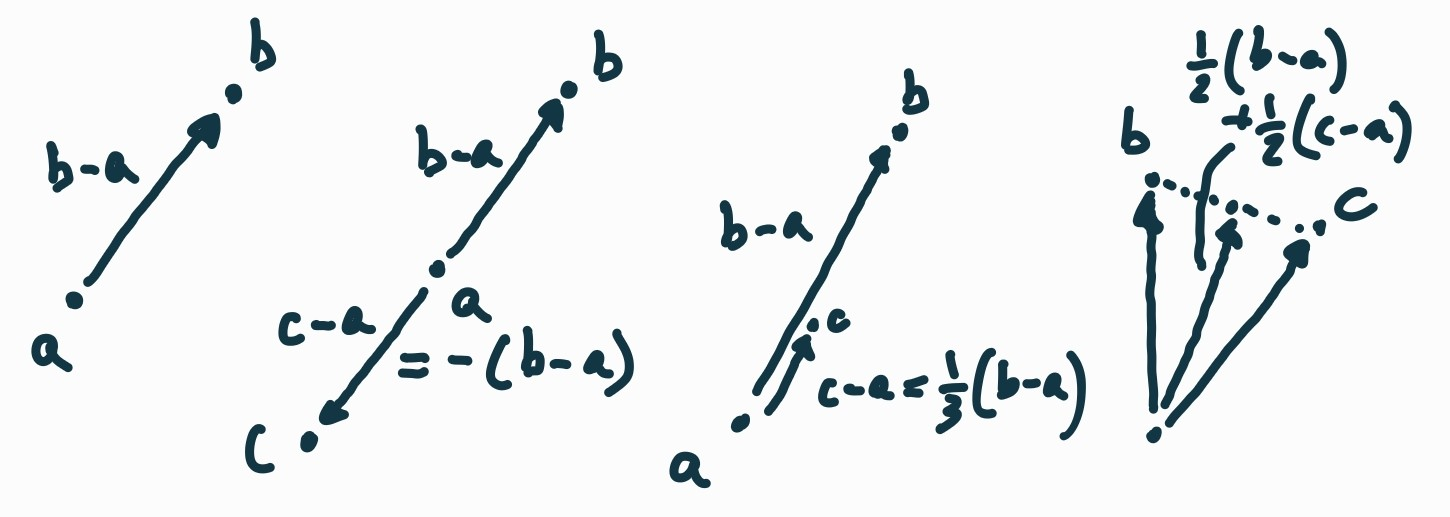
\includegraphics[width=0.7\textwidth]{tempimages/EnsembleDifferences.jpg}
	\caption{This picture represents the motivation of the definition of the operations on the space of differences.}\label{pm_es_vectorJustification}
\end{figure}

Figure \ref{pm_es_vectorJustification} shows the motivation of the construction. We take an ensemble $\ens[a]$ to be a reference, the origin. For any other ensemble $\ens[b]$, we imagine the change from $\ens[a]$ to $\ens[b]$ as the arrow the connects the first to the second. This is the ensemble difference $(\ens[b] - \ens[a])$. The inverse of that difference would find an ensemble $\ens[c]$ in the opposite direction. Note that $\ens[a]$ now sits exactly in between $\ens[b]$ and $\ens[c]$, and therefore $\ens[a] = \frac{1}{2}\ens[b] + \frac{1}{2}\ens[c]$ if and only if $(\ens[b] - \ens[a]) = - (\ens[c]- \ens[a])$. That is, relationship between vectors are re-expressed as convex combinations of ensembles.

Similarly, we can now stretch or shrink difference by a factor. For example, multiplying the difference by a third will give us the ensemble that it's at a third between $\ens[a]$ and $\ens[b]$. Similarly, we can add differences. For example, $\frac{1}{2}(\ens[b] - \ens[a]) + \frac{1}{2}(\ens[c] - \ens[a])$ will give us the difference $\left(\left(\frac{1}{2}\ens[b] + \frac{1}{2}\ens[c]\right) - \ens[a]\right)$. In other words, the difference with the midpoint between $\ens[b]$ and $\ens[c]$. Note that if we double that difference, we obtain the parallelogram law for vector addition.

Clearly, if we stretch a difference too much, we will go out of the ensemble space. Yet, since we can always shrink and then stretch,  all operations defined on differences within the ensemble space can be formally defined on differences that go outside the ensemble space. If $\ens[a]$ is an internal point, then differences exist in every direction. This is, in a nutshell, the vector space we are constructing. This clarifies that, in the end, we are always going to be interested in sets of vectors that can be shrunk within the ensemble space.\footnote{It is unclear whether this insight may help us understand what the topology of the embedding vector space is.}

While the motivation is straight-forward, the construction is complicated by the fact that there are multiple way of expressing the same difference. In the third example in figure \ref{pm_es_vectorJustification}, $(\ens[b] - \ens[a])$ and $3(\ens[c] - \ens[a])$ correspond to the same vector. Therefore, we need to specify this equivalence class and prove that the set of equivalence classes form a vector space. The way that the equivalence relationship is specified is so that the proofs remain short and manageable, and it is therefore mainly a technical issue.\footnote{Originally, the equivalence relationship we specified by three separate cases. While more directly justifiable, that gave 6 different possible combinations to check in every proof.}

\begin{mathSection}
	
	\begin{defn}[Ensemble differences]
		Given an ensemble space, a difference between two ensembles represents the change required to transform one ensemble into another. Formally, an \textbf{ensemble difference}, noted $r(\ens[b] - \ens[a])$, is a triple formed by a real number $r \in \mathbb{R}$ and an ordered pair of ensembles $\ens[a],\ens[b] \in \Ens$.
	\end{defn}
	
	\begin{defn}
		The \textbf{scalar multiplication} of a difference $s(\ens[b] - \ens[a])$ by a real number $r \in \mathbb{R}$, noted $r(s(\ens[b] - \ens[a]))$, is the difference $(rs)(\ens[b] - \ens[a])$
	\end{defn}
	
	\begin{defn}
		Two ensemble differences are \textbf{equivalent}, noted $r(\ens[b] - \ens[a]) \sim s(\ens[c] - \ens[a])$, if there exists $k \in \mathbb{R}$ such that
		$$ \frac{1}{r+s+k} (r \ens[b] + s \ens[a] + k \ens[a]) = \frac{1}{r+s+k} (s \ens[c] + r \ens[a] + k \ens[a]).$$
	\end{defn}
	
	\begin{remark}
		Note that this is an equation between affine combinations since the coefficients can be negative. The equality can be satisfies only if both affine combinations exist.
	\end{remark}
	
	\begin{coro}
		If the above condition is satisfied for some $k$, then it is satisfied for all $k \neq -(r+s)$ for which the affine combination exists.
	\end{coro}
	
	\begin{proof}
		Suppose $\frac{1}{r+s+k} (r \ens[b] + s \ens[a] + k \ens[a]) = \frac{1}{r+s+k} (s \ens[c] + r \ens[a] + k \ens[a])$ for some $k$. Let $k' \in \mathbb{R}$ be such that $\frac{1}{r+s+k'} (r \ens[b] + s \ens[a] + k' \ens[a])$ is a valid affine combination, which requires $r+s+k'\neq0$. Then we have $\frac{1}{r+s+k'} (r \ens[b] + s \ens[a] + k' \ens[a]) = \frac{1}{r+s+k'} (r \ens[b] + s \ens[a] + k \ens[a]) + \frac{k'-k}{r+s+k'} \ens[a] = \frac{r+s+k}{r+s+k'} \frac{1}{r+s+k}(r \ens[b] + s \ens[a] + k \ens[a]) + \frac{k'-k}{r+s+k'} \ens[a] = \frac{r+s+k}{r+s+k'} \frac{1}{r+s+k}(s \ens[c] + r \ens[a] + k \ens[a]) + \frac{k'-k}{r+s+k'} \ens[a] = \frac{1}{r+s+k'} (s \ens[c] + r \ens[a] + k' \ens[a])$.
	\end{proof}
	
	\begin{prop}
		Difference equivalence is reflexive, symmetric and transitive and therefore is an equivalence relation.
	\end{prop}
	
	\begin{proof}
		For reflexivity, we have $\frac{1}{r+r+k} (r \ens[b] + r \ens[a] + k \ens[a]) = \frac{1}{r+r+k} (r \ens[b] + r \ens[a] + k \ens[a])$, which is satisfied for any $\ens[a], \ens[b] \in \Ens$ and $r \in \mathbb{R}$.
		
		For symmetry, note that if $r$ is switched with $s$ and $\ens[b]$ with $\ens[c]$, the left side becomes the right side and vice-versa.
		
		For transitivity, suppose $r(\ens[b] - \ens[a]) \sim s(\ens[c] - \ens[a])$ and $s(\ens[c] - \ens[a]) \sim t(\ens[d] - \ens[a])$. Then for some $k$ and $l$ we have $\frac{1}{r+s+k} (r \ens[b] + s \ens[a] + k \ens[a]) = \frac{1}{r+s+k} (s \ens[c] + r \ens[a] + k \ens[a])$ and $\frac{1}{s+t+l} (s \ens[c] + t \ens[a] + l \ens[a]) = \frac{1}{s+t+l} (t \ens[d] + s \ens[a] + l \ens[a])$. Let $l' = r - t + k$ and therefore $k = t - r + l'$. We have $\frac{1}{r+s+k} (s \ens[c] + r \ens[a] + k \ens[a]) = \frac{1}{r+s+t-r} (s \ens[c] + r \ens[a] + (t-r +l') \ens[a]) = \frac{1}{s+t+l'} (s \ens[c] + t \ens[a] + l' \ens[a])$. Therefore $l'$ is such that $\frac{1}{s+t+l'} (s \ens[c] + t \ens[a] + l' \ens[a])$ is a valid affine combination, which means$\frac{1}{s+t+l'} (s \ens[c] + t \ens[a] + l' \ens[a]) =\frac{1}{s+t+l'} (t \ens[d] + s \ens[a] + l' \ens[a])$. Now let $k' = l' + s -r$ which gives $l' = k' + r -s$ and $k' = k + s - t$. We have $\frac{1}{r+t+k'} (r \ens[b] + t \ens[a] + k' \ens[a]) = \frac{1}{r+s+k} (r \ens[b] + s \ens[a] + k \ens[a]) = \frac{1}{r+s+k} (s \ens[c] + r \ens[a] + k \ens[a]) = \frac{1}{s+t+l'} (t \ens[d] + s \ens[a] + l' \ens[a]) = \frac{1}{r+t+k'} (t \ens[d] + r \ens[a] + k' \ens[a])$. Therefore $r(\ens[b] - \ens[a]) \sim t(\ens[d] - \ens[a])$.
	\end{proof}
	
	\begin{prop}\label{pm_es_ensDiffProps}
		The ensemble difference equivalence relation satisfies the following:
		\begin{enumerate}
			\item if $r(\ens[b] - \ens[a]) \sim s(\ens[c] - \ens[a])$ with $r\neq0$ and $s\neq0$, then $\ens[a]$, $\ens[b]$ and $\ens[c]$ are on the same line
			\item if $r\neq0$, $[r(\ens[b] - \ens[a])] = \left\{(r+j)\left(\left(\frac{r}{r+j}\ens[b] +\frac{j}{r+j} \ens[a]\right) -\ens[a]\right)\right\}$
			\item $\left[0(\ens[b] - \ens[a])\right] = \left\{0\left(\ens - \ens[a]\right) \, | \, \ens \in \Ens \right\} \cup \left\{r\left(\ens[a] - \ens[a]\right) \, | \, r \in \mathbb{R} \right\}$
			\item given $p \in (0,1]$, $r(\ens[b] - \ens[a]) \sim \frac{r}{p}((p\ens[b] + \bar{p}\ens[a]) - \ens[a])$
			\item $r(\ens[b] - \ens[a]) \sim s(\ens[c] - \ens[a])$ implies $(rt)(\ens[b] - \ens[a]) \sim (st)(\ens[c] - \ens[a])$ and therefore scalar multiplication maps equivalence classes to equivalence classes
		\end{enumerate}
	\end{prop}
	
	\begin{proof}
		For 1, the condition for equivalence imposes that an affine combination of $\ens[b]$ and $\ens[a]$ equals an affine combination of $\ens[c]$ and $\ens[a]$. Equivalently, this says that they are expressible as affine combinations of each other, that they are on the same line.
		
		For 2, let us first verify that $r(\ens[b] - \ens[a]) \sim (r+j)\left(\left(\frac{r}{r+j}\ens[b] +\frac{j}{r+j} \ens[a]\right) -\ens[a]\right)$. We have $\frac{1}{r+r+j+k} (r \ens[b] + (r+j) \ens[a] + k \ens[a]) = \frac{1}{r+r+j+k} \left((r+j)\left(\frac{r}{r+j}\ens[b] +\frac{j}{r+j} \ens[a]\right) + r \ens[a] + k \ens[a]\right)=\frac{1}{r+r+j+k} \left(r\ens[b] +j\ens[a] + r \ens[a] + k \ens[a]\right)$, which means the two differences are equivalent. Note that all ensembles that are on the same line of $\ens[a]$ and $\ens[b]$ can, except for $\ens[a]$, be expressed as $\frac{r}{r+j}\ens[b] +\frac{j}{r+j} \ens[a]$. Since, by 1, being on the same line is necessary condition for equivalence, the expression spans the entire equivalence class.
		
		For 3, we have $\frac{1}{r+k} (r \ens[b] + k \ens[a]) = \frac{1}{r+k} (r \ens[a] + k \ens[a])$. If $r=0$ we have $\ens[a] = \ens[a]$ which is satisfied for all $\ens[b], \ens[b] \in \Ens$. If $r\neq0$ we have $\frac{1}{r+k} (r \ens[b] + k \ens[a]) = \ens[a]$ which is satisfied only if $\ens[b] = \ens[a]$.
		
		For 4, let $\frac{r}{p}=r+j$. We have $j = \frac{r}{p}-r = \frac{r(1-p)}{p} = (r+j)\bar{p}$. Therefore $\frac{r}{r+j} = r\frac{p}{r} = p$ and $\frac{j}{r+j} = \bar{p}$. This matches the coefficients in the equivalence class.
		
		For 5, we have
		\begin{equation}
			\begin{aligned}
				\frac{1}{r+s+k} (r \ens[b] + s \ens[a] + k \ens[a]) &= \frac{1}{r+s+k} (s \ens[c] + r \ens[a] + k \ens[a]) \\
				\frac{1}{tr+ts+tk} (rt \ens[b] + st \ens[a] + kt \ens[a]) &= \frac{1}{rt+st+kt} (st \ens[c] + rt \ens[a] + kt \ens[a]) \\
				\frac{1}{tr+ts+k'} (rt \ens[b] + st \ens[a] + k' \ens[a]) &= \frac{1}{rt+st+k'} (st \ens[c] + rt \ens[a] + k' \ens[a])
			\end{aligned}
		\end{equation}
		which means $(rt)(\ens[b] - \ens[a]) \sim (st)(\ens[c] - \ens[a])$.
	\end{proof}
	
	\begin{defn}
		The \textbf{addition} between two equivalence classes of differences is defined by 
		$$\left[r(\ens[b] - \ens[a])\right] + \left[s(\ens[c] - \ens[a])\right] = \left[(r+s+k) \left(\left(\frac{r}{r+s+k}\ens[b] + \frac{s}{r+s+k} \ens[c] +\frac{k}{r+s+k} \ens[a] \right) - \ens[a]\right)\right]$$
		where $r+s+k \neq 0$.
	\end{defn}
	\begin{check}
		We need to show that the definition does not depend on the chosen representatives of the classes on the left hand side. We first check the case when both classes are of the form $[0(\ens[b] - \ens[a])]$. Suppose we have two elements of said equivalence class. Either the coefficient is zero or the two ensembles are the same. In either case, the elements on the right side of the definition of the addition will be affine combinations of $\ens[a]$ only. Therefore the result of the addition of $[0(\ens[b] - \ens[a])]$ with itself gives us $[0(\ens[b] - \ens[a])]$. Now suppose we sum an equivalence class $r[\ens[b] - \ens[a]]$ with $[0(\ens[c] - \ens[a])]$. Note that either $s=0$ or $\ens[c]=\ens[a]$. In either cases, the ensemble in the result is an affine combination of only $\ens[b]$ and $\ens[a]$ for every $k$. The result, then, span exactly the equivalence class of $r[\ens[b] - \ens[a]]$. Lastly, suppose we are summing two equivalence classes different from $[0(\ens[b] - \ens[a])]$. The ratio between $\ens[b]$ and $\ens[c]$ remains the same for all $k$, therefore the ensembles in the result span the line between $\ens$ and an affine combination of $\ens[b]$ and $\ens[c]$, which is means all elements fall in the same equivalence class.
	\end{check}
	
	\begin{coro}
		Let $\ens[a] \in \Ens$ be an ensemble and let $V = \{ [r(\ens[b]-\ens[a])] \}$ be the set of equivalence classes of ensemble differences from $\ens[a]$. Then the addition of ensemble difference over $V$ is a commutative monoid. If $\ens[a]$ is an internal point, the addition is an abelian group.
	\end{coro}
	
	\begin{proof}
		The operation is commutative as the definition of addition is symmetric over its arguments. The operation is associative as further sums of equivalence classes turn into additions of the real coefficients and extensions of affine combinations both of which are associative. The zero equivalence class $[0(\ens[b] - \ens[a])]$ is the identity element, as shown in the previous proof. The addition is a commutative monoid.
		
		Now let $\ens[a]$ is an internal point and let $[r(\ens[b] - \ens[a])]$ be an equivalence class. Since $\ens[a]$ is an internal point, we can find $\ens[c] \in \Ens$ such that $\ens[a] = p \ens[b] + \bar{p} \ens[c]$. Consider $\left[r\frac{\bar{p}}{p}(\ens[c] - \ens[a])\right]$. Note that $r + r\frac{\bar{p}}{p} = \frac{r}{p}(p+\bar{p}) = \frac{r}{p}$. The addition is given by
		\begin{equation}
			\begin{aligned}
				&\left[\left(r+r\frac{\bar{p}}{p}+k\right) \left(\left(\frac{r}{r+r\frac{\bar{p}}{p}+k}\ens[b] + \frac{r\frac{\bar{p}}{p}}{r+r\frac{\bar{p}}{p}+k} \ens[c] +\frac{k}{r+r\frac{\bar{p}}{p}+k} \ens[a] \right) - \ens[a]\right)\right] \\
				&=\left[\left(\frac{r}{p}+k\right) \left(\left(\frac{\frac{r}{p}}{\frac{r}{p}+k}(p\ens[b] + \bar{p} \ens[c]) +\frac{k}{\frac{r}{p}+k} \ens[a] \right) - \ens[a]\right)\right] \\
				&=\left[\left(\frac{r}{p}+k\right) \left(\left(\frac{\frac{r}{p}}{\frac{r}{p}+k}\ens[a] +\frac{k}{\frac{r}{p}+k} \ens[a] \right) - \ens[a]\right)\right] \\
				&= [0(\ens[b] - \ens[a])].
			\end{aligned}
		\end{equation}
		This means that $\left[r\frac{\bar{p}}{p}(\ens[c] - \ens[a])\right]$ is the inverse of $[r(\ens[b] - \ens[a])]$ and that the addition is an abelian group.
	\end{proof}
	
	\begin{thrm}[Differences form a vector space]
		Let $\ens[a] \in \Ens$ be an internal point and let $V = \{ [r(\ens[b]-\ens[a])] \}$ be the set of equivalence classes of ensemble differences from $\ens[a]$. Then $V$ is a vector space under scalar multiplication and addition.
	\end{thrm}
	
	\begin{proof}
		Scalar multiplication is compatible with the multiplication between scalars since $r(s(t(\ens[b] - \ens[a])))= r((st)(\ens[b]-\ens[a])) = (rst)(\ens[b]-\ens[a]) = (rs)(t(\ens[b]-\ens[a])$. The identity of the scalars is the identity of scalar multiplication since $1(r(\ens[b]-\ens[a])) = r(\ens[b] - \ens[a])$. Scalar multiplication is distributive with respect to vector addition
		\begin{equation}
			\begin{aligned}
				&t\left(\left[r(\ens[b] - \ens[a])\right] + \left[s(\ens[c] - \ens[a])\right]\right) \\
				&= t\left[(r+s+k) \left(\left(\frac{r}{r+s+k}\ens[b] + \frac{s}{r+s+k} \ens[c] +\frac{k}{r+s+k} \ens[a] \right) - \ens[a]\right)\right] \\
				&= \left[t(r+s+k) \left(\left(\frac{r}{r+s+k}\ens[b] + \frac{s}{r+s+k} \ens[c] +\frac{k}{r+s+k} \ens[a] \right) - \ens[a]\right)\right] \\
				&= \left[(tr+ts+tk) \left(\left(\frac{tr}{tr+ts+tk}\ens[b] + \frac{ts}{tr+ts+tk} \ens[c] +\frac{tk}{tr+ts+tk} \ens[a] \right) - \ens[a]\right)\right] \\
				&= \left[(tr+ts+k') \left(\left(\frac{tr}{tr+ts+k'}\ens[b] + \frac{ts}{tr+ts+k'} \ens[c] +\frac{k'}{tr+ts+k'} \ens[a] \right) - \ens[a]\right)\right] \\
				&\left[tr(\ens[b] - \ens[a])\right] + \left[ts(\ens[c] - \ens[a])\right].
			\end{aligned}
		\end{equation}
		Scalar multiplication is distributive with respect to scalar addition
		\begin{equation}
			\begin{aligned}
				&s\left[r(\ens[b] - \ens[a])\right] + t\left[r(\ens[b] - \ens[a])\right] \\
				&\left[sr(\ens[b] - \ens[a])\right] + \left[tr(\ens[b] - \ens[a])\right] \\
				&= \left[(sr+tr+k) \left(\left(\frac{sr}{sr+tr+k}\ens[b] + \frac{tr}{sr+tr+k} \ens[b] +\frac{k}{sr+tr+k} \ens[a] \right) - \ens[a]\right)\right] \\
				&= \left[(sr+tr+k) \left(\left(\frac{sr+tr}{sr+tr+k}\ens[b] + \frac{k}{sr+tr+k} \ens[a] \right) - \ens[a]\right)\right] \\
				&= [((s+t)r)(\ens[b]-\ens[a])] \\
				&= (s+t)[r(\ens[b]-\ens[a])].
			\end{aligned}
		\end{equation}
		Therefore $V$ with addition and scalar multiplication satisfies the definition of a vector space.
	\end{proof}
	
	\begin{defn}
		Given an internal point $\ens[a]$, the \textbf{natural embedding} of $\Ens$ into $V_{\ens[a]}$ is the map $\iota_{\ens[a]} : \Ens \hookrightarrow V_{\ens[a]}$, defined as $\iota_{\ens[a]}(\ens) \to [(\ens - \ens[a])]$, that maps each ensemble to its difference from $\ens[a]$.
	\end{defn}
	
	\begin{coro}
		The natural embedding of $\Ens$ into $V_{\ens[a]}$ preserves affine combinations. That is, $\iota\left(\sum_{i=1}^n r_i \ens_i \right) = \sum_{i=1}^n r_i \iota(\ens_i)$.
	\end{coro}
	
	\begin{proof}
		Let $r+s=1$, we have
		\begin{equation}
			\begin{aligned}
				r[(\ens[b] - \ens[a])] +s[(\ens[b] - \ens[a])] &= [r(\ens[b] - \ens[a])] +[s(\ens[b] - \ens[a])] \\
				&= \left[(r+s+k) \left(\left(\frac{r}{r+s+k}\ens[b] + \frac{s}{r+s+k} \ens[c] +\frac{k}{r+s+k} \ens[a] \right) - \ens[a]\right)\right] \\
				&= \left[(1+k) \left(\left(\frac{r}{1+k}\ens[b] + \frac{s}{1+k} \ens[c] +\frac{k}{1+k} \ens[a] \right) - \ens[a]\right)\right] \\
				&= \left[(1) \left(\left(\frac{r}{1}\ens[b] + \frac{s}{1} \ens[c] \right) - \ens[a]\right)\right] \\
				&= \left[\left(\left(r\ens[b] + s \ens[c] \right) - \ens[a]\right)\right].
			\end{aligned}
		\end{equation}
		If we apply recursively, we have $\sum_{i=1}^{n} r_i [(\ens_i - \ens[a])] = \left[\left(\left(\sum_{i=1}^{n}r_i \ens_i\right) - \ens[a]\right)\right]$. Therefore $\sum_{i=1}^n r_i \iota(\ens_i) = \iota\left(\sum_{i=1}^n r_i \ens_i \right)$.
	\end{proof}
	
	\begin{prop}
		Let $\ens[a],\ens[b] \in \Ens$ be two internal points. Then $r(\ens[c] - \ens[b]) \mapsto r(\ens[c]-\ens[a]) - r(\ens[b]-\ens[a])$ is an isomorphism between the corresponding vector spaces.
	\end{prop}
	
	\begin{proof}
		Note that the natural embedding of $\Ens$ in $V_{\ens[a]}$ and $V_{\ens[b]}$ are invertible, and therefore they give an affine map between $V_{\ens[a]}$ and $V_{\ens[b]}$. That is, $r(\ens[c] - \ens[b]) \mapsto r(\ens[c]-\ens[a])$ is an affine map. Moreover, $r(\ens[c] - \ens[b]) \mapsto r(\ens[c]-\ens[a]) - v$ will be an affine map for any $v \in V_{\ens[a]}$. An affine map is linear if and only if it maps the zero vector to the zero vector. Note that $r(\ens[v] - \ens[b])$ is the zero vector for $V_{\ens[b]}$ and which means the above map is affine if and only if $v = -r(\ens[b]-\ens[a])$.
	\end{proof}
\end{mathSection}

We leave open whether the ensemble space embeds continuously in a topological vector space, and whether the topological vector space would have to be a locally convex. The first step would be to check whether this is true in the finite dimensional case.

%\begin{mathSection}
%\begin{conj}\label{pm_es_ensemblesAreTVS}
%	An ensemble space embeds continuously in a topological vector space.
%\end{conj}

%\begin{remark}
%	Axioms of ensemble and mixture are not enough to guarantee the topological nature of the vector space. See \href{https://math.stackexchange.com/questions/4921905/cancellative-convex-spaces-and-topological-vector-spaces}{this post}. The issue is that we have no guarantee of continuity on the inverse (i.e. subtraction, multiplication by a negative number). As it is shown later, the entropy provides a pseudo-distance, which allows one to create open balls. Moreover, the entropy induces a metric tensor, which may induce a suitable topology.
%\end{remark}
%\end{mathSection}

\subsubsection{Self-mixtures}

As an example of a convex space that is non-cancellative, does not embed in a vector space, and therefore is ruled out as an ensemble space, we consider one in which the convex combination of two different elements returns the first. We show that this can be made to satisfy the axioms of ensemble and mixture, and therefore it is really the axiom of entropy that rules it out.

\begin{example}[Self-mixture]
	Let $\Ens = \{\ens[a], \ens[b]\}$ be a set endowed with the convex structure that satisfies identity, idempotence, commutativity and such that $p \ens[a] + \bar{p} \ens[b]$ equals $\ens[a]$ if $p=1$ and $\ens[b]$ otherwise. Identity, idempotence and commutativity are satisfied by construction. For associativity, note that the final result of multiple mixtures is $\ens[a]$ if and only if all elements of the mixtures are $\ens[a]$. The order does not matter, and therefore associativity is satisfied. Therefore such structure satisfies at least the axiom of mixture without the requirement of continuity.
	
	For continuity, we need to look at the inverse image under the mixing operation. Note that $+^{-1}(\emptyset) = \emptyset$ and $+^{-1}(\Ens) = [0,1] \times \Ens \times \Ens$. Since $\emptyset$ and $\Ens$ must be in any topology of $\Ens$, the continuity condition is satisfied for these sets. Next, we have  $+^{-1}(\{\ens[a]\}) = [0,1] \times \{\ens[a]\} \times \{\ens[a]\} \cup [1] \times \{\ens[a]\} \times \{\ens[b]\} \cup [0] \times \{\ens[b]\} \times \{\ens[a]\}$. Note that $[0]$ and $[1]$ are not open sets, therefore $\{\ens[a]\}$ cannot be in the topology of $\Ens$ or mixing would not be continuous. Finally, $+^{-1}(\{\ens[b]\}) = [0,1] \times \{\ens[b]\} \times \{\ens[b]\} \cup [0,1) \times \{\ens[a]\} \times \{\ens[b]\} \cup (0,1] \times \{\ens[b]\} \times \{\ens[a]\} = [0,1) \times \Ens \times \{\ens[b]\} \cup (0,1] \times \{\ens[b]\} \times \Ens$. Since $(0,1]$ and $[0,1)$ are open subsets of $[0,1]$, \{$\ens[b]\}$ can be an open set. Since the topology must be $\textsf{T}_0$, we must include at least $\{\ens[b]\}$ and therefore $\mathsf{T}_{\Ens} = \{\emptyset, \{\ens[b]\}, \{\ens[a], \ens[b]\}\}$ is a $\mathsf{T}_0$ second countable topology for which mixing is continuous. This means that the example satisfies both the axioms of ensemble and of mixture.
\end{example}

It is therefore the entropy that rules out this case. If the entropy of the two ensembles is different, it would jump from $S(\ens[a])$ directly to $S(\ens[b])$ for an infinitesimal mixture which violates the upper bound. If $S(\ens[a])$ equals $S(\ens[b])$, the entropy of the mixture of $\ens[a]$ and $\ens[b]$ is also the same, so the two ensembles cannot possibly be different by strict concavity.

Intuitively, this tells us that we cannot have a mixture of two different elements that happens to be equal to one of the original elements.

\begin{mathSection}
	\begin{coro}
		Let $\ens[a], \ens[b] \in \Ens$ such that $p\ens[a] + \bar{p} \ens[b] = \ens[b]$ for some $p \in (0,1]$. Then $\ens[a] = \ens[b]$. 
	\end{coro}
	
	\begin{proof}
		We have $p\ens[a] + \bar{p} \ens[b] = \ens[b] = p\ens[b] + \bar{p} \ens[b]$ for some $p \in (0,1]$. Therefore $\ens[a] = \ens[b]$.
	\end{proof}
\end{mathSection}

\subsection{Boundedness of lines}

Another constraint that the entropy imposes is that the ensemble space is bounded along every direction. That is, if we take two ensembles, these will identify an affine line in the embedding vector space that will, at some point, exit the ensemble space in both directions.

\begin{figure}[h]
	\centering
	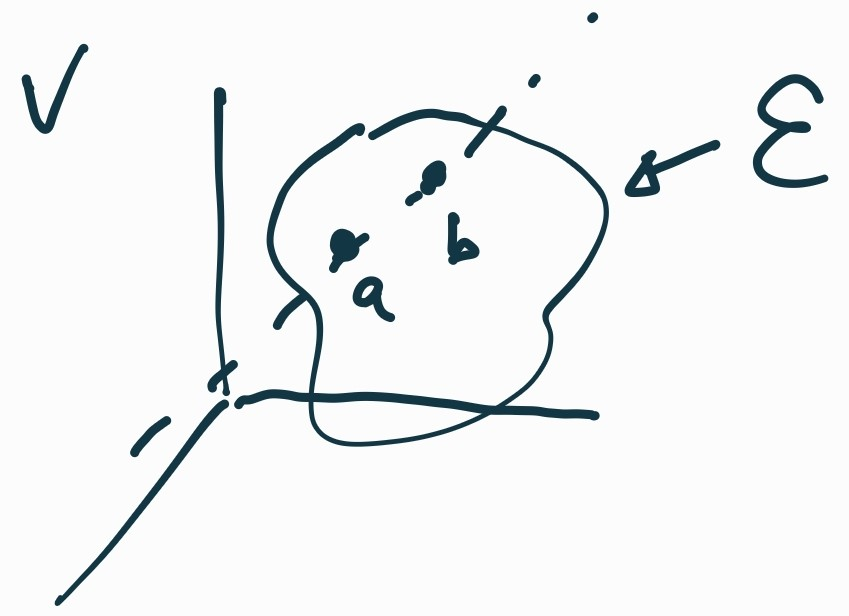
\includegraphics[width=0.4\textwidth]{tempimages/BoundedEnsembleSpace.jpg}
	\caption{$\Ens$ is the ensemble space and $V$ is the embedding vector space. Any affine line, like the dashed one in the picture, will intersect $\Ens$ over a finite range limited by the two elements $a$ and $b$ of the vector space (but not necessarily of the ensemble space).}
\end{figure}

The proof proceeds as follows. Suppose we take three points and assign them an entropy that is strictly concave: can we assign to always pick an entropy value that satisfies the bounds for any subsequent point? The answer is negative and figure \ref{pm_es_directionallyBound} represent the problem pictorially. On the horizontal axis we can imagine all the ensembles over a line, and on the vertical axis their entropy. We fix the entropy for the origin, the blue and the red point. What are the values for the next point, the green one, that satisfy the entropy bounds? Because of strict concavity, the green point must remain below the blue line. The green line represents the upper bound for the blue point, which means the green point must be above the purple line. If we go far enough, the blue and purple line meet, leaving no possible value for the entropy.

\begin{mathSection}
\begin{defn}
	A \textbf{line} $A \subseteq \Ens$ is a convex subset such that for any three elements one can be expressed as a mixture of the other two. That is, for all $\ens_1, \ens_2, \ens_3 \in A$ there exists a permutation $\sigma : \{1,2,3\} \to \{1,2,3\}$ and $p \in [0,1]$ such that $\ens_{\sigma(1)} = p \ens_{\sigma(2)} + \bar{p} \ens_{\sigma(3)}$.
\end{defn}

\begin{prop}
	Given $\ens[a], \ens[b] \in \Ens$, there is only one line that contains them.
\end{prop}

\begin{proof}
	Since an ensemble space embeds into a vector space, given two ensembles there is only one affine line that connects them. A line is the intersection of the affine line with the ensemble space.
\end{proof}

\begin{thrm}[Lines are bounded]
	Let $A \subseteq \Ens$ be a line. Then we can find a bounded interval $V \subseteq \mathbb{R}$ and an invertible function $f : A \to V$ such that $f(p \ens[a] + \bar{p} \ens[b]) = p f(\ens[a]) + \bar{p} f(\ens[b])$ for all $\ens[a], \ens[b] \in A$.
\end{thrm}

\begin{proof}
	Let $A \subseteq \Ens$ be a line. Pick $\ens_0, \ens_1 \in A$. For any $\ens[a] \in A$, we can find an affine expression between $\ens_0$, $\ens_1$ and $\ens[a]$. Rearranging the terms, we can always write $\ens[a] = \bar{x}\ens_0 + x\ens_1$ where $x \in \mathbb{R}$. Note that $x$ uniquely determines $\ens[a]$. Therefore we can define $f(\ens[a]) \mapsto x$, and it will be an invertible function.
	
	We can verify that, given $\ens[a], \ens[b] \in A$, we have
	\begin{equation}
		\begin{aligned}
			f(p\ens[a] + \bar{p} \ens[b]) &= f(p\bar{x}_a \ens_0 + px_a \ens_1 + \bar{p}\bar{x}_b \ens_0 + \bar{p}x_b \ens_1) = f((p\bar{x}_a + \bar{p}\bar{x}_b) \ens_0 + (px_a + \bar{p}x_b) \ens_1) \\
			&= px_a + \bar{p}x_b = pf(\ens[a]) + \bar{p}f(\ens[b]).
		\end{aligned}
	\end{equation}
	
	We are going to show that the image $V=f(A)$ must be a bounded set, or it would eventually violate the entropy bounds. Given a value $x \in V$, there will be an entropy value $S(f^{-1}(x))$ which we can write as a function of the real value $S(x)$. This function will need to satisfy continuity, strict concavity and the upper variability bound.

\begin{figure}[H]
	\centering
	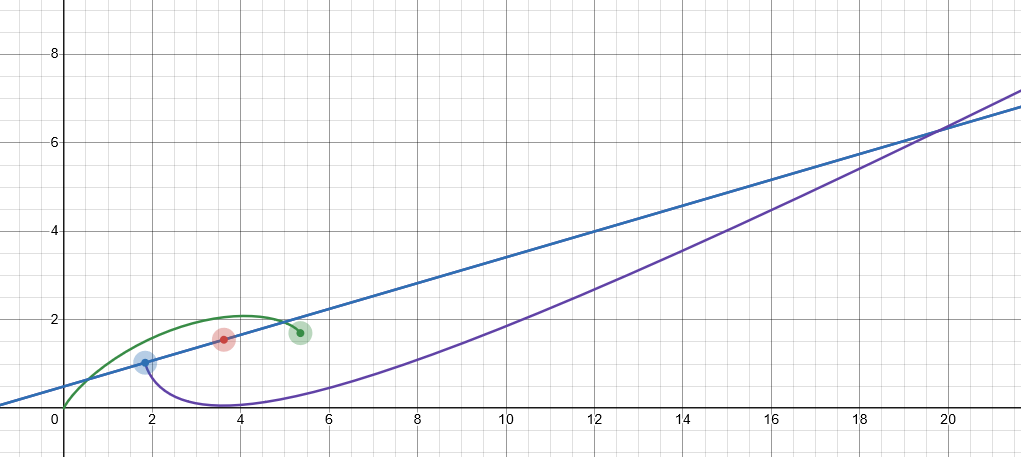
\includegraphics[width=0.7\textwidth]{tempimages/BoundsFromEntropy.png}
	\caption{Visual representation of the bounds. See proof for details.}\label{pm_es_directionallyBound}
\end{figure}
	We are going to show that the function $S(x)$ cannot extend to plus infinity. The same argument can be applied by symmetry for minus infinity. We are going to assume that $S(0) = 0$ without loss of generality. If $S$ is not defined at zero, or if the value is different, we can apply a translation on the argument or on the value, which will not affect the concavity of the function.
	
	Let $0 < a < b \in V$ be two distinct values, with $S(a)$ and $S(b)$ their respective entropies. We are going to show that if we pick a $c > b$ sufficiently large, we are not going to find a value for $S(c)$ that satisfies the bounds. In the picture, we have the three points, $a$ in blue, $b$ in red, $c$ in green. The horizontal axis represent the value, the position of the ensemble along the affine line, while the vertical axis represents the entropy. Consider the points $a$, $b$ and $c$. Since the entropy is strictly concave, $c$ must be placed under the blue line which represents an upper bound on $S(c)$. Now consider $0$, $a$ and $c$. Since $a$ is a mixture of $0$ and $c$, $S(a)$ will need to satisfy the upper bound given by $S(0)$ and $S(c)$. In the diagram, the green line represents the upper bound on $S(a)$ for the specific choice of $c$ and $S(c)$. Since $a$ and $S(a)$ are fixed, this puts a lower bound on $S(c)$, which is represented by the purple curve. That is, the purple curve represents the minimum value we have to assign to $S(c)$ such that $S(a)$ still satisfies the upper bound between $0$ and $c$. As the picture shows, the two bounds meet at some point and cannot both be satisfied.
	
	From strict concavity, noting that $\frac{c-b}{c-a} + \frac{b-a}{c-a} = 1$, we have:
	\begin{equation}
		\begin{aligned}
			S(b) &= S\left(\frac{c-b}{c-a} a + \frac{b-a}{c-a} c\right) > \frac{c-b}{c-a} S(a) + \frac{b-a}{c-a} S(c)\\
			(b-a)S(c) &< (c-a) S(b) - (c-b) S(a) = (c-a) S(b) - (c-a) S(a) + (b-a) S(a) \\
			S(c) &< \frac{S(b) - S(a)}{(b-a)} (c-a) + S(a) \\
		\end{aligned}
	\end{equation}
	
	From the upper bound, noting that $\frac{c-a}{c} + \frac{a}{c} = 1$ and recalling we assumed $S(0) = 0$, we have:
	\begin{equation}
		\begin{aligned}
			S(a) &= S\left(\frac{c-a}{c} 0 + \frac{a}{c} c\right) \leq I\left(\frac{c-a}{c}, \frac{a}{c}\right) + \frac{c-a}{c} S(0) +\frac{a}{c} S(c) \\
			\frac{a}{c} S(c) &\geq S(a) - I\left(\frac{c-a}{c}, \frac{a}{c}\right) \\
			S(c) &\geq \frac{c}{a} \left[ S(a) - I\left(\frac{c-a}{c}, \frac{a}{c}\right) \right]
		\end{aligned}
	\end{equation}
	
	Combining the bounds, we have:
	\begin{equation}
		\begin{aligned}
			\frac{S(b) - S(a)}{(b-a)} (c-a) + S(a) &> \frac{c}{a} \left[ S(a) - I\left(\frac{c-a}{c}, \frac{a}{c}\right) \right] \\
			(c-a) S(b) - (c-a)S(a) + (b-a) S(a) &> \frac{c(b-a)}{a} S(a) - \frac{c(b-a)}{a} I\left(\frac{c-a}{c}, \frac{a}{c}\right) \\
			a (c-a) S(b) - a(c-b) S(a) &> c(b-a)S(a) - c(b-a) I\left(\frac{c-a}{c}, \frac{a}{c}\right) \\
			a (c-a) S(b) + (-ac +ab -bc +ac) S(a) &> - c(b-a) I\left(\frac{c-a}{c}, \frac{a}{c}\right) \\
			a (c-a) S(b) -b (c-a) S(a) &> - c(b-a) I\left(\frac{c-a}{c}, \frac{a}{c}\right) \\
			a  S(b) - b S(a) &> - \frac{c(b-a)}{(c-a)} I\left(\frac{c-a}{c}, \frac{a}{c}\right) \\
		\end{aligned}
	\end{equation}
	
	Since $b > a$, $c > a$ and $I(p,\bar{p}) > 0$ for all $p \in (0,1)$, the right hand side of the inequality is always negative. As $c$ increases, the right hand side will go to zero, since $\lim\limits_{c\to \infty}\frac{c(b-a)}{c-a} = b-a$ and $\lim\limits_{c\to \infty} I\left(\frac{c-a}{c}, \frac{a}{c}\right) = I(1,0) = 0$. The left hand side is a constant. If the constant is positive, the inequality is always satisfied. If it is negative, it will not be satisfied for all $c$.
	
	From strict concavity, noting that $\frac{b-a}{b} + \frac{a}{b} = 1$, we have
	\begin{equation}
		\begin{aligned}
			S(a) &= S\left(\frac{b-a}{b} 0 + \frac{a}{b} b\right) > \frac{b-a}{b} S(0) + \frac{a}{b} S(b) = \frac{a}{b} S(b)\\
			b S(a) &> a S(b)  \\
			0 &> a S(b) - b S(a)\\
		\end{aligned}
	\end{equation}
	This shows that the left hand side of the previous inequality is negative, and therefore the bounds cannot be satisfied over the whole $\mathbb{R}$.
	
	This means that $V = f(A)$ must be bounded and therefore every line is a segment as embedded in the vector space.
\end{proof}

\begin{remark}
	Note that this does not mean that, along each direction, the line is closed in the vector space. That is, it may not include the extreme points. in the convex space. An open bounded interval, in fact, is still a convex space and we would be able to define an entropy on it.
\end{remark}
\end{mathSection}

The fact that the ensemble space is directionally bound gives us an intuitive property that we would, mistakenly, always think to be true. Suppose we have an ensemble $\ens$ and a sequence of ensembles $\ens[a]_i \in L$ on some line that contains $\ens$. Then $p_i \ens + \bar{p}_i \ens[a]_i \to \ens$ if $p_i \to 1$. This does not work in a convex space if directions are unbounded. For example, suppose $\ens = \mathbb{R}$, which is a convex set but not directionally bounded. Let $\ens = 0$, $\ens[a]_i = i$ and $p_i = 1 - \frac{1}{i}$. Then $\left(1 - \frac{1}{i}\right) 0 + \frac{1}{i}{i} = 1$. Therefore $p_i \ens + \bar{p}_i \ens[a]_i \nto \ens$. It is, again, the entropy that guarantee that this intuitive property is satisfied. \footnote{It is an open question whether this property is guaranteed for a generic sequence $\ens[a]_i$, not necessarily on a line.}

\begin{mathSection}
	\begin{prop}
		Let $L \subseteq \Ens$ be a line. Let $\ens \in L$ and $\ens[a]_i \in L$. Then $p_i \ens + \bar{p}_i \ens[a]_i \to \ens$ if $p_i \to 1$.
	\end{prop}
	
	\begin{proof}
		Pick $\ens[a] \in L$ such that $\ens[a] \neq \ens$. Then every $\ens[a]_i$ can be expressed as an affine combination $\ens[a]_i = r_i \ens + \bar{r}_i \ens[a]$. We have $p_i \ens + \bar{p}_i \ens[a]_i = p_i \ens + \bar{p}_i \left( r_i \ens + \bar{r}_i \ens[a] \right) = \left( p_i + \bar{p}_i r_i \right) \ens + \bar{p}_i\bar{r}_i \ens[a]$. Since the ensemble space is directionally bounded, the sequence $r_i$ is bounded from below and above. This means that $\bar{p}_i \to 0$ implies $p_i + \bar{p}_i r_i \to 1$ and $\bar{p}_i\bar{r}_i \to 0$. Therefore by continuity $\left( p_i + \bar{p}_i r_i \right) \ens + \bar{p}_i\bar{r}_i \ens[a] \to 1 \ens + 0 \ens[a] = \ens$.
	\end{proof}
\end{mathSection}

%TODO: for topology, the ensemble space is a convex neighbourhood of the origin, which means it is an absorbing set.

%\begin{prop}
%	The ensemble space is, as a subset of the embedding vector space, a radial set and, since the vector space is real, an absorbing set.
%\end{prop}

%\begin{proof}
%	Let $\ens[a] \in \Ens$ be an internal point and $\Ens \subseteq V_{\ens[a]}$ be the ensemble space as a subset of the embedding vector space. Since $\ens[a]$ is an internal point, for every direction there exist a finite segment that starts from $\ens[a]$ and proceeds in that direction. Therefore the ensemble space is a radial set. Moreover, since in a real vector space \href{https://en.wikipedia.org/wiki/Radial_set#Relation_to_absorbing_sets}{every radial is absorbing}, the ensemble space is an absorbing set. TODO: find a better reference.
%\end{proof}

\section{Entropic geometry}

In this section we will see how the entropy imposes a geometric structure on the ensemble space. The core idea is that, since the entropy is strictly concave, its Hessian is negative definite. The negation is therefore a positive definite, real-valued function of two variations and plays the role of a metric tensor.

\subsection{Mixing entropy as pseudo-distance}

The first observation is that the entropy can be used to define a pseudo-distance. If we mix two ensembles, in fact, the average entropy cannot decrease, and will stay the same if the two components of the mixture are the same ensemble. The increase, then, is zero if the two ensembles are equal, greater than zero if not, with the maximum if they are orthogonal. This means that the increase of entropy during mixing can be used to characterize how different two ensembles are.

We define the mixing entropy as the increase in entropy for the equal mixture of two states. This satisfies all axioms for a distance, except the triangle inequality. The mixing entropy recovers the Jensen-Shannon divergence in both the classical and quantum case, and can therefore be seen as its generalization.

\begin{mathSection}
\begin{defn}
	Given two ensembles $\ens[a], \ens[b] \in \Ens$, the \textbf{mixing entropy}, also called Jensen-Shannon divergence, is the increase in entropy associated to their equal mixture. That is:
	$$MS(\ens[a], \ens[b]) = S\left(\frac{1}{2}\ens[a] + \frac{1}{2} \ens[b]\right) - \left(\frac{1}{2} S(\ens[a]) + \frac{1}{2} S(\ens[b])\right).$$
\end{defn}

\begin{prop}
	The mixing entropy $MS(\ens[a], \ens[b])$ satisfies the following:
	\begin{enumerate}
		\item \textbf{non-negativity}: $MS(\ens[a], \ens[b]) \geq 0$
		\item \textbf{identity of indiscernibles}: $MS(\ens[a], \ens[b]) = 0 \iff \ens[a]=\ens[b]$
		\item \textbf{unit boundedness}: $MS(\ens[a], \ens[b]) \leq 1$
		\item \textbf{maximality of orthogonals}: $MS(\ens[a], \ens[b]) = 1 \iff \ens[a] \ortho \ens[b]$
		\item \textbf{symmetry}: $MS(\ens[a], \ens[b]) = MS(\ens[b], \ens[a])$
	\end{enumerate}
\end{prop}

\begin{proof}
	For 1, by strict concavity, $S\left(\frac{1}{2} \ens[a] + \frac{1}{2} \ens[b]\right) \geq \frac{1}{2} S(\ens[a]) + \frac{1}{2} S(\ens[b])$, which means $S\left(\frac{1}{2} \ens[a] + \frac{1}{2} \ens[b]\right) - \left(\frac{1}{2} S(\ens[a]) + \frac{1}{2} S(\ens[b])\right) = MS(\ens[a], \ens[b]) \geq 0$.
	
	For 2, the concavity is strict and therefore the equality holds if and only if $\ens[a] = \ens[b]$.
	
	For 3, by the upper variability bound, $S\left(\frac{1}{2} \ens[a] + \frac{1}{2} \ens[b]\right) \leq I(\frac{1}{2}, \frac{1}{2}) + \frac{1}{2} S(\ens[a]) + \frac{1}{2} S(\ens[b])$, which means $S\left(\frac{1}{2} \ens[a] + \frac{1}{2} \ens[b]\right) - \left(\frac{1}{2} S(\ens[a]) + \frac{1}{2} S(\ens[b])\right) = MS(\ens[a], \ens[b]) \leq I(\frac{1}{2}, \frac{1}{2}) = 1$.
	
	For 4, the upper variability bound is saturated if and only if $\ens[a] \ortho \ens[b]$.
	
	For 5, by commutativity of mixing and of addition the definition of the mixing entropy is symmetric.
\end{proof}

\begin{prop}
	In discrete and continuous classical cases, the mixing entropy coincides with the Jensen-Shannon divergence. In quantum spaces it coincindes with the quantum Jensen-Shannon divergence.
\end{prop}

\begin{proof}
	Looking at the definitions of the \href{https://en.wikipedia.org/wiki/Jensen%E2%80%93Shannon_divergence}{Jensen-Shannon divergence}, in the classical case we have
	$$ JSD(\ens[a], \ens[b]) = S\left(\frac{1}{2}\ens[a] + \frac{1}{2}\ens[b] \right)  - \frac{1}{2} \left(S(\ens[a]) + S(\ens[b])\right) = MS(\ens[a], \ens[b]),$$
	and, similarly, in the quantum case we have
	$$ QJSD(\ens[a], \ens[b]) = S\left(\frac{1}{2}\ens[a] + \frac{1}{2}\ens[b] \right)  - \frac{1}{2} \left(S(\ens[a]) + S(\ens[b])\right) = MS(\ens[a], \ens[b]).$$
\end{proof}

\begin{remark}
	The mixing entropy fails to be a distance function as it does not satisfy the triangle inequality. In the classical and quantum case, in fact, the JSD and QJSD are the square of a distance function. Given the current axiom, it is unlikely that this result can be generalized to the mixing entropy itself. The issue is that we do not have enough information about the relative entropy of 3 points, apart from the orthogonal case. It is very likely that, on physics ground, there should be constraints on the mixing entropy between three points.
\end{remark}
\end{mathSection}

Though the mixing entropy is not a distance function, we can still show that, like a distance, it decreases as one ensemble approaches another. The notion of two ensembles approaching is given by the convex structure: a convex space a mixture of $\ens[a]$ and $\ens[b]$ is closer to $\ens[a]$ than $\ens[b]$.

\begin{mathSection}
\begin{prop}
	Let $\ens[a], \ens[b] \in \Ens$. Then $MS(\ens[a], \ens[b]) \geq MS(\ens[a], p\ens[a]+\bar{p}\ens[b])$ with the equality holding if and only if $p=0$ or $\ens[a] = \ens[b]$.
\end{prop}

\begin{proof}
	First let us show that $\frac{1}{2} \ens[a] + \frac{1}{2} \ens[b]$ can be expressed as a mixture of $\frac{1}{2} \ens[a] + \frac{1}{2}\left(p\ens[a] + \bar{p} \ens[b]\right)$ and $p\ens[a] + \bar{p} \ens[b]$.
	\begin{equation}
		\begin{aligned}
			\frac{1}{2} \ens[a] + \frac{1}{2} \ens[b] &=  \frac{1-2p}{1-p}\left[\frac{1}{2} \ens[a] + \frac{1}{2}\left(p\ens[a] + \bar{p} \ens[b]\right)\right] + \frac{p}{1-p}\left[p\ens[a] + \bar{p} \ens[b]\right] \\
			&= \left( \frac{1-2p}{1-p} \frac{1+p}{2} + \frac{2}{2} \frac{p^2}{1-p} \right) \ens[a] + \left( \frac{1-2p}{1-p} \frac{\bar{p}}{2}+ \frac{2}{2} \frac{p\bar{p}}{1-p} \right) \ens[b] \\
			&= \frac{1}{2} \frac{1-2p + p - 2p^2 + 2p^2}{1-p} \ens[a] + \frac{1}{2}\left(1-2p+2p\right) \ens[b] = \frac{1}{2} \ens[a] + \frac{1}{2} \ens[b]
		\end{aligned}
	\end{equation}
	From strict concavity we have
	\begin{equation}
		\begin{aligned}
			S\left(\frac{1}{2} \ens[a] + \frac{1}{2} \ens[b] \right) &\geq  \frac{1-2p}{1-p}S\left(\frac{1}{2} \ens[a] + \frac{1}{2}\left(p\ens[a] + \bar{p} \ens[b]\right)\right) + \frac{p}{1-p} S\left(p\ens[a] + \bar{p} \ens[b]\right).
		\end{aligned}
	\end{equation}
	Note that the equality holds only if $p=0$, in which case the second mixing coefficient is zero.
	
	Now let us show that $p \ens[a] + \bar{p} \ens[b]$ can be expressed as a mixture of $\frac{1}{2} \ens[a] + \frac{1}{2}\left(p\ens[a] + \bar{p} \ens[b]\right)$ and $\ens[b]$.
	\begin{equation}
		\begin{aligned}
			p \ens[a] + \bar{p} \ens[b] &= \frac{2p}{1+p}\left[\frac{1}{2} \ens[a] + \frac{1}{2}\left(p\ens[a] + \bar{p} \ens[b]\right)\right] + \frac{1-p}{1+p} \ens[b] \\
			&= \frac{2p}{1+p} \frac{1+p}{2} \ens[a] + \left( \frac{2p}{1+p} \frac{\bar{p}}{2}+ \frac{\bar{p}}{1+p} \right) \ens[b] \\
			&= p \ens[a] + \bar{p} \frac{p+1}{1+p}\ens[b] = p \ens[a] +\bar{p} \ens[b]
		\end{aligned}
	\end{equation}
	From strict concavity we have
	\begin{equation}
		\begin{aligned}
			S\left(p \ens[a] + \bar{p} \ens[b] \right)&\geq \frac{2p}{1+p} S\left(\frac{1}{2} \ens[a] + \frac{1}{2}\left(p\ens[a] + \bar{p} \ens[b]\right)\right) + \frac{1-p}{1+p} S(\ens[b]) \\
			-S(\ens[b]) &\geq \frac{1+p}{1-p} \frac{2p}{1+p} S\left(\frac{1}{2} \ens[a] + \frac{1}{2}\left(p\ens[a] + \bar{p} \ens[b]\right)\right) - \frac{1+p}{1-p} S\left(p \ens[a] + \bar{p} \ens[b] \right) \\
			&= \frac{2p}{1-p} S\left(\frac{1}{2} \ens[a] + \frac{1}{2}\left(p\ens[a] + \bar{p} \ens[b]\right)\right) - \frac{1+p}{1-p} S\left(p \ens[a] + \bar{p} \ens[b] \right).
		\end{aligned}
	\end{equation}
	Note that the equality holds only if $p=0$, in which case the first mixing coefficient is zero.
	
	Putting it all together
	\begin{equation}
		\begin{aligned}
			MS(\ens[a],\ens[b]) &= S\left(\frac{1}{2} \ens[a] + \frac{1}{2} \ens[b]\right)- \frac{1}{2} S(\ens[a]) - \frac{1}{2} S(\ens[b]) \\
			&\geq \frac{1-2p}{1-p}S\left(\frac{1}{2} \ens[a] + \frac{1}{2}\left(p\ens[a] + \bar{p} \ens[b]\right)\right) + \frac{p}{1-p} S\left(p\ens[a] + \bar{p} \ens[b]\right) - \frac{1}{2} S(\ens[a]) \\
			&+ \frac{1}{2}\left[\frac{2p}{1-p} S\left(\frac{1}{2} \ens[a] + \frac{1}{2}\left(p\ens[a] + \bar{p} \ens[b]\right)\right) - \frac{1+p}{1-p} S\left(p \ens[a] + \bar{p} \ens[b] \right)\right] \\
			&= \left(\frac{1-2p + p}{1-p}\right)S\left(\frac{1}{2} \ens[a] + \frac{1}{2}\left(p\ens[a] + \bar{p} \ens[b]\right)\right) - \frac{1}{2} S(\ens[a]) + \frac{1}{2}\left(\frac{2p-1-p}{1-p}\right) S\left(p\ens[a] + \bar{p} \ens[b]\right) \\
			&= S\left(\frac{1}{2} \ens[a] + \frac{1}{2}\left(p\ens[a] + \bar{p} \ens[b]\right)\right) - \frac{1}{2} S(\ens[a]) - \frac{1}{2} S\left(p\ens[a] + \bar{p} \ens[b]\right) \\
			&= MS(\ens[a], p\ens[a] + \bar{p} \ens[b]).
		\end{aligned}
	\end{equation}
	The equality holds only if $p=0$.
\end{proof}
\end{mathSection}

The fact that the mixing entropy decreases on all directions as we get closer to an ensemble allows us to create a notion of open ball, which allows to prove the topology is at least $\mathsf{T}_1$. The lack of the triangle inequality does not allow us to easily prove that we can always find disjoint balls centered at two different points, which is what typically is used to show that the topology is Hausdorff.\footnote{It is likely that we could at least show that in the finite dimensional case the topology is the standard one on $\mathbb{R}^n$, and that the embedding of the ensemble space into $\mathbb{R}^n$ is continuous.}

\begin{mathSection}
\begin{defn}
	Given $\ens[a] \in \Ens$ and $r \in [0,1]$, an entropic open ball is the set of all ensembles for which the mixing entropy from $\ens[a]$ is within $r$. That is, $B_r(\ens[a]) = \{\ens \in \Ens \, | \, MS(\ens[a], \ens) < r\}$.
\end{defn}
\begin{coro}
	Every entropic open ball is an open set.
\end{coro}

\begin{proof}
	Since both the entropy and the mixing operation are continuous, the mixing entropy is also continuous. An entropic open ball is the reverse image of an open set through a continuous function and it is therefore an open set.
\end{proof}

\begin{prop}
	Ensemble spaces are Hausdorff topological spaces.
\end{prop}

\begin{proof}
	We will prove this in two ways. First, since the topology is second countable, the space is Hausdorff if and only if limits of sequences are unique. Let $\ens[a]_i$ be a sequence such that $\ens[a]_i \to \ens[a]$ and $\ens[a]_i \to \ens[b]$. We have $MS(\ens[a]_i, \ens[a]_i) = 0 \to 0$. Since $MS$ is continuous, we also have $MS(\ens[a]_i, \ens[a]_i) \to MS(\ens[a], \ens[b])$ which means $MS(\ens[a], \ens[b]) = 0$ and therefore $\ens[a] = \ens[b]$.
	
	Another way to show it, a space is Hausdorff if and only if any singleton $\{\ens\}$ is the intersection of all closed neighborhoods of $\ens$. For any $\ens$, the intersection of all closed neighborhoods will contain $\ens$, so we just need to show that no other elements can be in all closed neighborhood. Consider an entropic closed ball centered around $\ens$ with radius $r>0$. It will contain an entropic open ball of the same radius and is therefore a closed neighborhood of $\ens$. Given an element $\ens[a] \neq \ens$, a closed ball with radius less than $MS(\ens, \ens[a])$ will not contain $\ens[a]$. Therefore, the only element contained in all entropic closed balls is $\ens$, which means the intersection of all closed neighborhoods of $\ens$ contains only $\ens$.
\end{proof}

\begin{remark}
	Intuitively, we would expect the entropic balls to be convex. This intuition is supported by numeric calculation for both the \href{https://www.desmos.com/calculator/ama0u3u31d}{classical case} and the \href{https://www.desmos.com/calculator/6ga2hygwmm}{quantum case} (though the quantum case is not checked for a three dimensional quantum system). However, the current axioms allow us to use a different entropy function in a space that is not orthogonally decomposable: the extreme points are not orthogonal. In this case, one is able to create open balls that are not convex.
	
	Whether this is physically relevant or not depends on whether there are additional physical constraints on the mixing entropy between three points, which is very likely.
\end{remark}


\begin{prop}
	Let $U \subseteq \Ens$ be an open set. Let $\ens[a] \in U$ and $L \subseteq \Ens$ be a line containing $\ens[a]$. Then there is an $r \in (0,1]$ such that for all $\ens \in L$ such that $MS(\ens[a], \ens) < r$ we have $\ens \in U$.
\end{prop}

\begin{proof}
	Let $U \subseteq \Ens$ be an open set, $\ens[a] \in U$ and $L \subseteq \Ens$ be a line containing $\ens[a]$. Take $\ens[b] \in L$ such that $\ens[b] \neq \ens[a]$. Let $f : [0,1] \to \Ens$ be such that $f(p) \mapsto p \ens[a] + \bar{p} \ens[b]$. Since the mixing operation is continuous, then $f$ is also continuous. This means that $f^{-1}(U)$ is an open subset of $[0,1]$. Since $\ens[a] \in U$, $1 \in f^{-1}(U)$ and therefore there will be an open interval $(\lambda, 1]$ such that $(\lambda, 1] \subseteq f^{-1}(U)$. Let $\ens[c] = \lambda \ens[a] + \bar{\lambda} \ens[b]$ and $r = MS(\ens[a], \ens[c])$. We have that, for all $p \in (0,1)$, $MS(\ens[a], p\ens[a] +\bar{p}\ens[c])<r$. We also have $p\ens[a] +\bar{p}\ens[c] = p\ens[a] +\bar{p}(\lambda \ens[a] + \bar{\lambda} \ens[b]) = (p + \bar{p}\lambda)\ens[a] + \bar{p}\bar{\lambda}\ens[b]$ where $p + \bar{p}\lambda = p + \lambda - p\lambda = \lambda - p\bar{\lambda} \geq \lambda$. Therefore $p\ens[a] +\bar{p}\ens[c] \in f((\lambda,1]) \subseteq U$.
	
	If $\ens[a]$ is an extreme point of $L$ (i.e. there is no $\ens[d] \in L$ such that $p\ens[b] + \bar{p}\ens[d] = \ens[a]$), then we are done. If $\ens[a]$ is not an extreme point, then we can find $\ens[d] \in L$ such that $p\ens[b] + \bar{p}\ens[d] = \ens[a]$. Repeat the previous procedure with $\ens[d]$ to find another $r'$ and the $t$ be the minimum between the two. Then we have that $t \in (0,1]$ such that for all $\ens \in L$ such that such that $MS(\ens[a], \ens) < r$, $\ens \in U$.
\end{proof}
\end{mathSection}
	
There are a number of conjectures on the topology generated by the entropic open ball that are probably all related. They are summarized here with some notes on what was understood:

\begin{conj}
	For every sequence $\ens[a]_i \in \Ens$, $\ens[a]_i \to \ens[a]$ if and only if $MS(\ens[a], \ens[a]_i) \to 0$.
\end{conj}

\begin{conj}
	The topology of the ensemble space is generated by the entropic open balls.
\end{conj}

\begin{conj}
	Let $U \subseteq \Ens$ be an open set and $\ens[a] \in U$. Then we there exists an $r \in (0,1]$ such that $B_r(\ens[a]) \subseteq U$.
\end{conj}

\begin{remark}
	These conjectures are likely the same. If the topology is generated by the entropic open balls, then convergence in mixing entropy is the convergence criteria associated with the topology. It also means that we can generate every open set with entropy open balls by fitting them insight every open set.
	
	Note that all entropic open balls are open sets in the topology, since the mixing entropy is a continuous function. It suffices to prove that all open sets can be generated by open balls. We have shown that given a point in an open set we can find a finite range of mixing entropy along each direction. However, since we do not know if there is a non-zero infimum across all directions, we do not know whether we can ``fit'' an entropic open ball.
	
	Similarly, it is clear that if a sequence converge, the mixing distance goes to zero. However, we do not know whether there is an open set for which the mixing entropy goes to zero but the sequence does not converge. This would mean that a sequence is always eventually enters an entropic open ball of any size, but it may not enter all open sets.
\end{remark}

\begin{conj}
	Let $\ens[a], \ens[b]_i\in \Ens$ and $\ens[c]_i = p \ens[a] +\bar{p} \ens[b]_i$ for some $p \in (0,1)$. Then $\ens[b]_i \to \ens[b]$ if and only if $\ens[c]_i \to \ens[c]$. 
\end{conj}

\begin{conj}[Affine combinations are continuous]
	Let $\ens \in \Ens$ and let $p \in [0,1]$. Let $+_{p\ens[a]} : \Ens \to \Ens$ be the curried function $+_{p\ens[a]}(\ens[b]) = p\ens[a] + \bar{p}\ens[b]$. The function is a homeomorphism between $\Ens$ and $+_{p\ens[a]}(\Ens)$.
\end{conj}

\begin{conj}
	Mixing is an open map.
\end{conj}

\begin{conj}
	An ensemble embeds continuously into a topological vector space.
\end{conj}

\begin{conj}
	Let $+_{\ens[a]\ens[b]} : [0,1] \to \Ens$ be the curried function $+_{\ens[a]\ens[b]}(p) = p\ens[a] + \bar{p}\ens[b]$. The function is a homeomorphism between $[0,1]$ and $+_{\ens[a]\ens[b]}([0,1])$.
\end{conj}

\begin{remark}
	These are all about showing that mixing allows a continuous inverse. It is easy to show that mixing gives us a continuous bijection. The problem is showing that the inverse is continuous.
	
	Continuity of mixtures only shows that we can stretch open sets to bigger open sets. What we would need is to show that we can shrink open sets to open sets. For example, suppose $U$ is an open neighborhood of $\ens[a]$. The set $V = p \ens[a] + \bar{p} U$ is a set that contains $\ens[a]$ and it is a strict subset of $V$. The question is whether a sequence can stay in $U$, converge to $\ens[a]$ without ever entering $V$.
\end{remark}

Another open question is whether the mixing entropy, or the entropy directly, can be related to a generalized notion of inner product.

\subsection{Entropic metric}

The second observation is that the strict concavity of the entropy forces the Hessian to be negative definite. The negation of the Hessian, then, is a positive definite function of two variations. In general, the Hessian of a scalar function is not a tensor. However, the ensemble space is a linear space and that linearity has physical significance. It is only for coordinates linear with respect to the mixing coefficient that the convex combination of coordinates will equal the statistical mixture of the corresponding ensembles. Therefore the metric tensor corresponds to the Hessian calculated on that linear structure. When using non-linear coordinates, as long as the coordinates are smooth, one can always make the appropriate transformation to linear coordinates.

\begin{mathSection}
\begin{remark}
	In this section we will assume that an ensemble space embeds continuously into a topological vector space, even though we have not yet proved it. We are going to talk about variations $\delta \ens$ on the space, even though it is not yet clear exactly which mathematical approach is best to make variations well-defined. We are also going to talk about a metric tensor even though the space is not, in general, a manifold. All these issues will need to be resolved in due time.
\end{remark}
	
\begin{defn}
	An ensemble space is \textbf{smooth} if the entropy is twice differentiable with respect to the mixing coefficients.
\end{defn}

\begin{prop}
	Discrete and continuous classical ensemble spaces and quantum ensemble spaces are smooth.
\end{prop}

\begin{proof}
	In both the discrete classical case and the quantum case the entropy of an ensemble is the Shannon entropy of a decomposition in terms of pure states. The Shannon entropy is a smooth function of the coefficients. For the continuous classical case, the differential entropy is a smooth function of the probability density, which is linear under mixture. Therefore the entropy is always smooth with respect to mixing coefficients.
\end{proof}

\begin{defn}
	Assuming $\Ens$ embeds in a topological vector space and given $\ens \in \Ens$, a \textbf{variation} $\delta \ens$ of $\ens$ is a vector in the ambient space such that $\forall t \in [0,1]$ $\ens + t \delta \ens \in \Ens$. Unless otherwise noted, we assume the variation is expressed on the affine structure. Note that it can be re-expressed through a non-linear map as long as the map is differentiable (i.e. it maps variations to variations).
\end{defn}

\begin{remark}
	Note that since an ensemble space is a convex subset of a real vector space, coordinate systems that are linear with respect to the vector space are privileged. It is only in these coordinates, in fact, that linear combinations correspond to mixtures. The strict concavity of the entropy is therefore guaranteed in these coordinates and only these coordinates. Given the special physical significance of these coordinates, all differential objects and properties will be defined in these coordinates.
\end{remark}

\begin{defn}
	Given an ensemble $\ens \subseteq \Ens$ and a variation $\delta \ens$ defined at that point, the \textbf{norm} of $\delta \ens$ is given by
	$$ \lVert \delta \ens \rVert_{\ens} = \sqrt{ 8 MS(\ens, \ens + \delta \ens) }.$$
	The \textbf{metric tensor} (i.e. the inner product between $\delta \ens_1 , \delta \ens_2 \in T_{\ens}$) is given by
	$$ g_{\ens}( \delta \ens_1, \delta \ens_2 ) = \frac{1}{2} \left( \lVert \delta \ens_1 + \delta \ens_2 \rVert_{\ens}^2 - \lVert \delta \ens_1 \rVert_{\ens}^2 - \lVert \delta \ens_2 \rVert_{\ens}^2 \right).$$
\end{defn}

\begin{thrm}
	Let $\Ens$ be a smooth ensemble space. Then, on the affine structure, we have
	$$ \lVert \delta \ens \rVert_{\ens}^2 = - \frac{\partial^2 S}{\partial \ens^2}(\delta \ens , \delta \ens) $$
	and 
	$$ g_{\ens}( \delta \ens_1, \delta \ens_2 ) = - \frac{\partial^2 S}{\partial \ens ^2}( \delta \ens_1, \delta \ens_2 ).$$
\end{thrm}

\begin{proof}
	To recover the first two expressions, we simply have to calculate the leading term. Since the entropy is twice differentiable, on the affine structure, we can expand it as
	\begin{equation}
		\begin{aligned}
			S(\ens + \delta \ens) &= S(\ens) + \frac{\partial S}{\partial \ens} \delta \ens + \frac{1}{2} \frac{\partial^2 S}{\partial \ens^2} \delta \ens \delta \ens + O(\delta \ens ^3).
		\end{aligned}
	\end{equation}
	Expanding the definition of $MS$, we have
	\begin{equation}
		\begin{aligned}
			MS(\ens, \ens + \delta \ens) &= S\left(\frac{1}{2} \ens + \frac{1}{2}(\ens + \delta \ens) \right) - \frac{1}{2} S(\ens) - \frac{1}{2} S(\ens+\delta \ens) \\
			&=  S\left(\ens + \frac{1}{2} \delta \ens \right) - \frac{1}{2} S(\ens) - \frac{1}{2} S(\ens+\delta \ens) \\
			&= S(\ens) + \frac{\partial S}{\partial \ens} \frac{1}{2}\delta \ens + \frac{1}{2} \frac{\partial^2 S}{\partial \ens^2} \frac{1}{2}\delta \ens \frac{1}{2}\delta \ens + O(\delta \ens ^3) \\
			&- \frac{1}{2} S(\ens) - \frac{1}{2} \left( S(\ens) + \frac{\partial S}{\partial \ens} \delta \ens + \frac{1}{2} \frac{\partial^2 S}{\partial \ens^2} \delta \ens \delta \ens + O(\delta \ens ^3) \right) \\
			&= S(\ens) + \frac{1}{2} \frac{\partial S}{\partial \ens} \delta \ens + \frac{1}{8} \frac{\partial^2 S}{\partial \ens^2} \delta \ens \delta \ens \\
			&- S(\ens) - \frac{1}{2} \frac{\partial S}{\partial \ens} \delta \ens - \frac{1}{4} \frac{\partial^2 S}{\partial \ens^2} \delta \ens \delta \ens + O(\delta \ens ^3) \\
			&= - \frac{1}{8} \frac{\partial^2 S}{\partial \ens^2} \delta \ens \delta \ens + O(\delta \ens ^3).
		\end{aligned}
	\end{equation}
	
	Therefore
	$$ \lVert \delta \ens \rVert^2 = 8 MS(\ens, \ens + \delta \ens) = -  \frac{\partial^2 S}{\partial \ens^2} (\delta \ens, \delta \ens).$$
	
	We can now substitute the norm in the definition of the metric tensor. We have
	\begin{equation}
		\begin{aligned}
			g_{\ens}(\delta \ens_1, \delta \ens_2 ) &= \frac{1}{2} \left( \lVert \delta \ens_1 + \delta \ens_2 \rVert^2 - \lVert \delta \ens_1 \rVert^2 - \lVert \delta \ens_2 \rVert^2 \right) \\
			&= \frac{1}{2} \left( - \frac{\partial^2 S}{\partial \ens^2} (\delta \ens_1 + \delta \ens_2, \delta \ens_1 + \delta \ens_2) + \frac{\partial^2 S}{\partial \ens^2} (\delta \ens_1, \delta \ens_1) + \frac{\partial^2 S}{\partial \ens^2} (\delta \ens_2, \delta \ens_2) \right) \\
			&= - \frac{1}{2} \left(  \frac{\partial^2 S}{\partial \ens^2} (\delta \ens_1, \delta \ens_1) + \frac{\partial^2 S}{\partial \ens^2} (\delta \ens_1, \delta \ens_2) + \frac{\partial^2 S}{\partial \ens^2} (\delta \ens_2, \delta \ens_1) + \frac{\partial^2 S}{\partial \ens^2} (\delta \ens_2, \delta \ens_2) \right. \\
			&-  \left. \frac{\partial^2 S}{\partial \ens^2} (\delta \ens_1, \delta \ens_1) - \frac{\partial^2 S}{\partial \ens^2} (\delta \ens_2, \delta \ens_2) \right) \\
			&= - \frac{\partial^2 S}{\partial \ens^2} (\delta \ens_1, \delta \ens_2). \\
		\end{aligned}
	\end{equation}
\end{proof}
\end{mathSection}

We now show that the metric tensor we defined reduces to the Fisher-Rao metric in the classical case and to its quantum equivalent in the quantum case.

\begin{mathSection}
\begin{prop}
	For a continuous classical ensemble space, the metric corresponds to the Fisher-Rao metric.
\end{prop}

\begin{proof}
	Let $\Ens$ be a continuous classical ensemble space. Each ensemble is a classical probability density $\rho$. Let $V \subseteq \Ens$ be a manifold of probability distributions over $X$ parametrized by $\theta^i$. The \href{https://en.wikipedia.org/wiki/Fisher_information_metric}{Fisher-Rao metric} is defined as:
	\begin{equation}
		g_{ij} =- \int_X \frac{\partial^2 \log \rho}{\partial \theta^i \partial \theta^j} \rho dx.
	\end{equation}
	where $\log$ will be the natural logarithm throughout this calculation. Recall that for a continuous classical ensemble, the entropy is given by
	\begin{equation}
		S(\rho) =- \int_X \rho \log \rho dx.
	\end{equation}
	
	Let us now calculate the first two terms in the Taylor expansion around $\rho$ with a variation $\delta\rho$. Recall that
	\begin{equation}
		\begin{aligned}
			\log(x+dx) &= \log(x) + d_x \log x \, dx + \frac{1}{2} d_x d_x  \log x \, dx^2 + O(dx^3) \\
			&= \log(x) + \frac{1}{x} dx - \frac{1}{2} \frac{1}{x^2} dx^2 + O(dx^3).
		\end{aligned}
	\end{equation}
	We have
	\begin{equation}
		\begin{aligned}
			S(\rho + \delta \rho) &= -\int_X (\rho + \delta \rho) \log (\rho + \delta \rho) dx \\
			&=-\int_X (\rho + \delta \rho) \left[\log \rho + \frac{1}{\rho} \delta \rho - \frac{1}{2\rho^2} \delta \rho^2 + O(\delta \rho^3)\right] dx \\
			&= - \int_X \rho \log \rho dx - \int_X \left[\log \rho + 1 \right]dx \delta \rho -\int_X \left[\frac{1}{\rho} - \frac{\rho}{2\rho^2}\right] dx \delta \rho^2 + \int_X dx O(\delta\rho^3) \\
			&= - \int_X \rho \log \rho dx - \int_X \left[\log \rho + 1 \right]dx \delta \rho - 	
			\frac{1}{2}\int_X \frac{1}{\rho} dx \delta \rho^2 + \int_X dx O(\delta\rho^3) \\
		\end{aligned}
	\end{equation}
	\begin{equation}
		\begin{aligned}
			\frac{\partial^2 S}{\partial \rho^2}(\delta \rho, \delta \rho) &= -\int_X \frac{1}{\rho} \delta \rho^2 dx = -\int_X \frac{1}{\rho} \delta \rho^2 dx + 0 = -\int_X \frac{1}{\rho} \delta \rho^2 dx + \delta^2 (1) \\
			&= -\int_X \frac{1}{\rho} \delta \rho^2 dx + \delta^2 \int_X \rho dx = -\int_X \frac{1}{\rho} \delta \rho^2 dx + \int_X \delta^2 \rho dx \\
			&= \int_X \rho dx \left[-\frac{1}{\rho^2} \delta \rho^2 + \frac{1}{\rho} \delta^2 \rho \right]
			= \int_X \rho dx \, \delta \left[\frac{1}{\rho} \delta \rho \right] \\
			&= \int_X \rho dx \, \delta^2 \log \rho.
		\end{aligned}
	\end{equation}
	
	Let us consider a family of ensembles charted by a set of parameters $\theta^i$, not necessarily forming a linear chart. We have
	\begin{equation}
		\begin{aligned}
			g_{\ens}(d\theta^i, d\theta^j) &= - \frac{\partial^2 S}{\partial \rho^2}\left(\frac{\partial 
				\rho}{\partial \theta^i} d\theta^i, \frac{\partial 
				\rho}{\partial \theta^j} d\theta^j\right) = - \int_X \rho dx \frac{\partial^2 \log \rho}{\partial \theta^i \partial \theta^j}d\theta^i d\theta^j
		\end{aligned}
	\end{equation}
	which recovers the Fisher-Rao metric.
\end{proof}

TODO: add a note/proof for the discrete version

\begin{remark}
	For quantum mechanics, the situation is more complicated as there are different definitions of Fisher metrics (see \href{https://arxiv.org/pdf/2008.11178}{RLD Fisher Information Bound for Multiparameter
		Estimation of Quantum Channels} or \href{https://link.springer.com/chapter/10.1007/978-4-431-54493-7_4}{Quantum Estimation Theory}). We will therefore just show a general connection, without worrying about the mathematical details.
	
\end{remark}

\begin{prop}
	For a quantum ensemble space, the metric corresponds to the Bures metric and the Quantum Fisher information metric.
\end{prop}

\begin{proof}
	Since we are working in a quantum ensemble space, each ensemble is a density operator $\rho$. The entropy is given by the von Neumann entropy
	\begin{equation}
		S(\rho) = - \tr\left(\rho \log \rho\right).
	\end{equation}
	We take the first variation and have
	\begin{equation}
		\begin{aligned}
			\delta S(\rho) &= - \delta \tr\left(\rho \log \rho\right)= - \tr\left(\delta \rho \log \rho + \rho \delta \log \rho\right) \\
			&= - \tr\left(\delta \rho \log \rho + \rho \rho^{-1} \delta \rho \right) \\
			&= - \tr\left(\left(\log \rho + 1 \right) \delta \rho \right).
		\end{aligned}
	\end{equation}
	We take the second variation and have
	\begin{equation}
		\begin{aligned}
			\delta^2 S(\rho) &= - \delta \tr\left(\left(\log \rho + 1 \right) \delta \rho \right) \\
			&= - \tr\left(\delta \left(\log \rho + 1 \right) \delta \rho + \left(\log \rho + 1 \right) \delta \delta \rho \right) \\
			&= - \tr\left(\rho^{-1} \delta \rho \delta \rho + \left(\log \rho + 1 \right) \delta \delta \rho \right).
		\end{aligned}
	\end{equation}
	Note that $\delta \rho$ is defined in a linear chart, therefore $\delta \delta \rho = 0$. Therefore we have 
	\begin{equation}
		\begin{aligned}
			\frac{\partial^2 S}{\partial \rho^2}(\delta \rho, \delta \rho) &= - \tr\left(\rho^{-1} \delta \rho \delta \rho \right).
		\end{aligned}
	\end{equation}
	Let us consider a family of ensembles charted by a set of parameters $\theta^i$, not necessarily forming a linear chart. We have
	\begin{equation}
		\begin{aligned}
			g_{\ens}(d\theta^i, d\theta^j) &= - \frac{\partial^2 S}{\partial \rho^2}\left(\frac{\partial 
				\rho}{\partial \theta^i} d\theta^i, \frac{\partial 
				\rho}{\partial \theta^j} d\theta^j\right) = \tr\left( \rho^{-1} \frac{\partial \rho}{\partial \theta^i }\frac{\partial \rho}{\partial \theta^j}\right) d\theta^i d\theta^j
		\end{aligned}
	\end{equation}
	which recovers one version of the Fisher-Rao metric.
	
	Recalling that the right logarithmic derivative (RLD) $L^R$ satisfies $\frac{\partial \rho}{\partial \theta} = \rho L^R$, we can write 
	\begin{equation}
		\begin{aligned}
			g_{\ens}(d\theta^i, d\theta^j) &= \tr\left( \rho^{-1} \frac{\partial \rho}{\partial \theta^i }\frac{\partial \rho}{\partial \theta^j}\right) d\theta^i d\theta^j = \tr(\rho^{-1}\rho L^R
			_i \rho L^R_j)d\theta^i d\theta^j = \tr(\rho L^R
			_i L^R_j)d\theta^i d\theta^j
		\end{aligned}
	\end{equation}
	which recovers the RLD Fisher information.
\end{proof}

\begin{remark}
	The feedback we received on the above derivation is contradictory, as some says we are handling the possible non-commutativity between $\rho$ and its variation $\delta \rho$ correctly and others say we aren't. Note that in all steps we are using the cyclical nature of the trace, and not commuting $\rho$ and its variation $\delta \rho$.
\end{remark}

\begin{remark}
	Note that these results relate also to the \href{https://en.wikipedia.org/wiki/Ruppeiner_geometry}{Ruppeiner metric}, which is the Hessian of the entropy. They also relate to the Hessian metric as described in  \href{https://web.osu.cz/~Zusmanovich/seminar/2017/wolak/ostrava-11-17-hessian-pdf.pdf}{Hessian structures} \href{https://link.springer.com/chapter/10.1007/978-3-642-40020-9_4}{1}.
\end{remark}
\end{mathSection}

\section{State capacity}

In this section we are going to develop a generalized version of the count of states. In classical statistical mechanics, the entropy for a uniform distribution $\rho_U$ over a region of phase space $U$ is given by $S(\rho_U) = \log \mu(U)$, where $\mu$ is the count of states given by the Liouville measure. Since entropy is our stating point: we will define the state capacity of a set of ensembles as the highest exponential of the entropy achievable by mixing those ensembles. This definition works in general, and recovers both the classical Liouville measure and the dimensionality of a quantum subspace.

Given an ensemble, we want to quantify the number of distinguishable cases over which the ensemble is spread. Since entropy characterizes the variability of the preparations of the ensemble, greater variability means the ensemble is spread over more cases. Therefore the count of distinguishable states must be a monotonic function of the entropy. The question is what function.

The first hint that the exponential is the right function is the relationship $S(\rho_U) = \log \mu(U)$ in classical statistical mechanics. Another hint is that we will want this size to be multiplicative over independent distributions. That is, if we have two ensembles $\rho_1 \in \Ens_1$ and $\rho_2 \in \Ens_2$ of two different ensemble spaces, we can imagine the composite system $\rho = \rho_1 \rho_2$ representing the ensemble of the two independent ensembles. While the entropy should be additive, that is $S(\rho) = S_1(\rho_1) + S_2(\rho_2)$, the count of states should be multiplicative, that is $\mu(\rho) = \mu_1(\rho_1) \mu_2(\rho_2)$. This suggests the relationship $S(\rho) = \log \mu (\rho)$ for all ensembles. The other hint is that the spread can be, at most, additive. If we mix two ensembles, the spread can be at most over the configurations of both and not more. The following shows that the exponential of the entropy has exactly that property.\footnote{
	Note that the state capacity for a single element corresponds to the ``ensemble volume'' defined in \href{https://arxiv.org/pdf/physics/9903045}{this work} and more recently \href{https://arxiv.org/pdf/1804.01343}{here}. It is connected to various uncertainty relationships, including a stronger form of the quantum uncertainty principle. It would be interesting to understand what results can be generalized to the ensemble space.}

\begin{mathSection}
\begin{prop}[Exponential entropy subadditivity]\label{pm_es_exponentialEntropySubadditivity}
	Let $\ens[a], \ens[b] \in \Ens$ and $\ens = p \ens[a] + \bar{p} \ens[b]$ for some $p \in [0,1]$. Then $2^{S(\ens)} \leq 2^{S(\ens[a])} + 2^{S(\ens[b])}$, with the equality holding if and only if $\ens[a] \ortho \ens[b]$ and $p = \frac{2^{S(\ens[a])}}{2^{S(\ens[a])} + 2^{S(\ens[b])}}$.
\end{prop}

\begin{proof}
	If $p$ is fixed, the upper variability bound of entropy is saturated only if $\ens[a]$ and $\ens[b]$ are orthogonal by definition. Therefore the entropy maximum for the mixed ensemble will be achieved when the elements are orthogonal, for some value of $p$.
	
	Now fix the entropy of $\ens[a]$ and $\ens[b]$ to some values $S_a = S(\ens[a])$ and $S_b = S(\ens[b])$. The entropy of the mixture depends only on $p$, so we need to find the $p$ that maximizes the expression. Since $\ens[a]$ and $\ens[b]$ are orthogonal, $S(p \ens[a] + \bar{p}\ens[b]) =  - p \log p - \bar{p} \log \bar{p} + p S_a + \bar{p} S_b$ which is a smooth function of $p$.
	\begin{equation}
		\begin{aligned}
			0 &= \frac{d}{dp} S(p \ens[a] + \bar{p}\ens[b]) =\frac{d}{dp} \left( - p \log p - \bar{p} \log \bar{p} + p S_a + \bar{p} S_b \right) \\
			&= - \log p - 1 + \log \bar{p} + 1 + S_a - S_b \\
			\log \frac{p}{\bar{p}} &= \log 2^{S_a} - \log 2^{S_b} \\
			\log \frac{p}{1-p} &= \log \frac{2^{S_a}}{2^{S_b}}  \\
			p 2^{S_b} &= (1-p) 2^{S_a}  \\
			p (2^{S_a} + 2^{S_b}) &= 2^{S_a}  \\
			p &= \frac{2^{S_a}}{2^{S_a} + 2^{S_b}}  \\
		\end{aligned}
	\end{equation}
	Note that since the entropy is strictly concave, the stationary point must correspond to a maximum. Having found the value of $p$ that maximizes the entropy, we can calculate the maximum entropy.
	\begin{equation}
		\begin{aligned}
			\bar{p} &= 1- \frac{2^{S_a}}{2^{S_a} + 2^{S_b}} = \frac{2^{S_b}}{2^{S_a} + 2^{S_b}} \\
			S(p \ens[a] + \bar{p}\ens[b]) &= - p \log p - \bar{p} \log \bar{p} + p S_a + \bar{p} S_b  \\
			&= - \frac{2^{S_a}}{2^{S_a} + 2^{S_b}} \log \frac{2^{S_a}}{2^{S_a} + 2^{S_b}} - \frac{2^{S_b}}{2^{S_a} + 2^{S_b}} \log \frac{2^{S_b}}{2^{S_a} + 2^{S_b}} \\
			&+ \frac{2^{S_a}}{2^{S_a} + 2^{S_b}} \log 2^{S_a} + \frac{2^{S_b}}{2^{S_a} + 2^{S_b}} \log 2^{S_b} \\
			&= \frac{2^{S_a}}{2^{S_a} + 2^{S_b}} \log \left( 2^{S_a} + 2^{S_b} \right) + \frac{2^{S_b}}{2^{S_a} + 2^{S_b}} \log \left( 2^{S_a} + 2^{S_b} \right) \\
			&= \frac{2^{S_a} + 2^{S_b}}{2^{S_a} + 2^{S_b}} \log \left( 2^{S_a} + 2^{S_b} \right) \\
			\log 2^{S(p \ens[a] + \bar{p}\ens[b])} &= \log \left( 2^{S_a} + 2^{S_b} \right) \\
			2^{S(p \ens[a] + \bar{p}\ens[b])} &=  2^{S_a} + 2^{S_b}  \\
		\end{aligned}
	\end{equation}
	Therefore the maximum entropy obtainable through a mixture is $S(p \ens[a] + \bar{p}\ens[b]) = \log (2^{S(\ens[a])} + 2^{S(\ens[b])})$ which is obtained when $\ens[a]$ and $\ens[b]$ are orthogonal and $p = \frac{2^{S(\ens[a])}}{2^{S(\ens[a])} + 2^{S(\ens[b])}}$.
\end{proof}

\begin{remark}
	We have proved that the exponential of the entropy gives us subadditivity. Ideally, we should prove that this is the only function with that characteristic.
\end{remark}

\begin{conj}
	Let $f : \mathbb{R} \to \mathbb{R}$ be a continuous function such that $f(S(p\ens[a]+\bar{p}\ens[b])) \leq f(S(\ens[a])) + f(S(\ens[b]))$ and the equality can be verified in some condition. Then $f(x) = \kappa^x$ for some arbitrary constant $\kappa$.
\end{conj}
\end{mathSection}

Given a set of ensembles, we can ask what spread is reachable by a mixture in terms of the number of distinguishable states. We call this the state capacity as it represents the maximum potential spread reachable by the set, and because it turns out to be a non-additive measure.\footnote{In some literature, capacities are non-additive measures.} The state capacity is monotone, subadditive and recovers additivity over orthogonal sets.

\begin{mathSection}
\begin{defn}
	Let $A \subseteq \Ens$ be a subset of an ensemble space. The \textbf{state capacity} of $A$ is defined as $\capacity(A) = \sup(2^{S(\hull(A))}\cup\{0\})$.
\end{defn}

\begin{check}
	Note that the supremum is taken on the extended real line, therefore it can be infinity. Therefore the state capacity is always defined.
\end{check}

\begin{coro}
	The state capacity can be equivalently defined on the $\sigma$-hull or the closed hull. That is, $\sup(2^{S(\hull(A))}\cup\{0\}) = \sup(2^{S(\shull(A))}\cup\{0\}) = \sup(2^{S(\chull(A))}\cup\{0\})$.
\end{coro}

\begin{proof}
	Any ensemble $\ens[a] \in \chull(A)$ is the limit of a sequence $\ens[a]_i \in \hull(A)$. Given that the entropy is continuous, $2^{S(\ens(a))} = \lim_{i \to \infty} 2^{S(\ens[a]_i)} \leq \sup(2^{S(\{\ens[a]_i\})}) \leq \sup(2^{S(\hull(A))})$. The supremum for the closed hull, then, cannot be greater than the supremum of the finite hull. Since the closed hull contains the finite hull, the supremum of the finite hull cannot be greater than the closed hull. Therefore, they must be the same. Since the $\sigma$-hull is a subset of the closed hull and a superset of the finite hull, its supremum will also be the same.
\end{proof}

\begin{prop}
	The state capacity is a set function that is
	\begin{enumerate}
		\item non-negative: $\capacity(A) \in [0, +\infty]$
		\item monotone: $A \subseteq B \implies \capacity(A) \leq \capacity(B)$
		\item subadditive: $\capacity(A \cup B) \leq \capacity(A) + \capacity(B)$
		\item additive over orthogonal sets: $A \ortho B \implies \capacity(A \cup B) = \capacity(A) + \capacity(B)$ 
	\end{enumerate}
\end{prop}

\begin{proof}
	1. The state capacity takes a subset of $\Ens$ and returns a real value and is therefore a set function. The exponential can only return non-negative values, therefore the state capacity of a set is non-negative. 
	
	2. The $\hull$ is a monotone function. The image of a set through a map is a monotone function. The supremum is a monotone function. Therefore the state capacity is a monotone function.
	
	3. Let $A, B \subseteq \Ens$ and let $\ens = p \ens[a] + \bar{p} \ens[b]$ for some $p \in [0,1]$, $\ens[a] \in A$ and $\ens[b] \in B$. By \ref{pm_es_exponentialEntropySubadditivity} and the definition of state capacity, $2^{S(\ens)} \leq 2^{S(\ens[a])} + 2^{S(\ens[b])} \leq \capacity(A) + \capacity(B)$. Since this is true for any finite mixture of elements of $A$ and $B$, it will be true for any element of $\hull(A \cup B)$. Consequently, the supremum of the exponential entropy cannot exceed the sum of the state capacities. Therefore $\capacity(A \cup B) \leq \capacity(A) + \capacity(B)$ (i.e. the state capacity is subadditive).
	
	4. Let $A, B \subseteq \Ens$ be two orthogonal subsets. Let $\{\ens[a]_i\} \subseteq A$ be a sequence of ensembles such that $2^{S(\ens[a]_i)} \to \capacity(A)$ and let $\{\ens[b]_i\} \subseteq B$ be a sequence of ensembles such that $2^{S(\ens[b]_i)} \to \capacity(B)$. Consider $\ens_i = p_i \ens[a]_i + \bar{p_i} \ens[b]_i$ where $p_i = \frac{2^{S(\ens[a]_i)}}{2^{S(\ens[a]_i)} + 2^{S(\ens[b]_i)}}$. Then, by \ref{pm_es_exponentialEntropySubadditivity}, $2^{S(\ens_i)} = 2^{S(\ens[a]_i)} + 2^{S(\ens[b]_i)}$. This means that $2^{S(\ens_i)} \to \capacity(A) + \capacity(B)$. Therefore $\capacity(A \cup B)$ must be at least $\capacity(A) + \capacity(B)$. Combining with the previous result, $\capacity(A \cup B) = \capacity(A) + \capacity(B)$. Therefore the state capacity, as a set function, is additive over orthogonal sets of ensembles.
\end{proof}

\begin{prop}
	The state capacity is continuous from above and below.
\end{prop}

\begin{proof}
	Let $\{A_i\} \subseteq \Sigma_{\Ens}$ be an increasing sequence. Given that the state capacity is monotone, $\{\capacity(A_i)\}$ is a an increasing sequence and it will converge in the extended real line. Let $A = \lim\limits_{i \to \infty} A_i$. We have $A = \cup A_i$ and $A_i \subseteq A$ for all $i$. Since state capacity is monotone, $\capacity(A_i) \leq \capacity(A)$ for all $i$ and therefore $\lim\limits_{i \to \infty} \capacity(A_i) \leq \capacity(A)$. Given any $\ens[a] \in \chull(A)$, we can find a sequence $\ens[a]_i \in \chull(A_i)$ such that $\ens[a]_i \to \ens[a]$. Because of the continuity of the entropy, $S(\ens[a]_i) \to S(\ens[a])$. This means we cannot have $k$ such that $\capacity(A) > k > \capacity(A_i)$ for all $i$, and therefore $\lim\limits_{i \to \infty} \capacity(A_i) = \capacity(A)$.
	
	The same argument works for decreasing sequences by inverting the order.
\end{proof}

\end{mathSection}

The state capacity is additive over orthogonal set. Intuitively, orthogonal sets corresponds to mutually exclusive events, so it makes sense that the count of states is additive. Intuitively, the converse should be true as well: if the count of states is additive, the sets correspond to mutually exclusive events and therefore the sets are orthogonal. This leads to the following conjecture

\begin{conj}
	The state capacity is additive only on orthogonal sets. That is, if $\capacity(A)<\infty$, $\capacity(B)<\infty$ and $\capacity(A \cup B) = \capacity(A) +\capacity(B)$, then $A \ortho B$.
\end{conj}

One should be able to prove that if the state capacity adds, then the states with highest entropy satisfy the upper variability bound and are orthogonal. What needs to be shown is that this is enough to say all elements are orthogonal. There is a series of nice results connected to this to expand the whole theory. If $\ens[a] \ortho \ens[b]$ then $\ens[a]$ is orthogonal to all the components of $\ens[b]$. If $\ens[a]$ is the ensemble with maximum entropy in $\chull(A)$, it should be true that all elements of the hull are components of $\ens[a]$. One should be able to show that, given two sequences with a convergent entropy and whose elements are orthogonal to each other, one can create another sequence that converges to an entropy higher than both of them. Another useful tool would be a type of sequence within $\hull(A)$ whose entropy always increases, tends to the supremum and each element is a component of the following. Also: the state with maximal entropy (it if exists) is an internal point. All internal points are in the $\sigma$-hull. We leave these series of conjecture for future work.

We now show that the state capacity recovers a notion of number of cases in all three target spaces. In the discrete classical case it recovers the number of points; in the continuous classical case, it recovers the Liouville volume; in the quantum case, it recovers the number of orthogonal pure states.

\begin{mathSection}
\begin{prop}
	Let $\Ens$ be a discrete classical ensemble space. Let $U \subseteq \{s_i\}$ be a subset of the corresponding (extreme) points and $A$ be the set of probability distributions whose support is a subset of $U$. Then $\capacity(A) = \#U$.
\end{prop}

\begin{proof}
	Let $A$ be the set of probability distributions defined over a discrete countable set $U$. The highest entropy is achieved by the uniform distribution, which equals $\log (\#U)$. Therefore $\capacity(A) = 2^{\log(\#U)} = \#U$.
\end{proof}

\begin{prop}
	Let $\Ens$ be a continuous classical ensemble space. Let $U \subseteq X$ be a subset of the corresponding symplectic manifold (i.e. phase space) and $A$ be the set of probability distributions whose support is a subset of $U$. Then $\capacity(A) = \mu(U)$ where $\mu(U)$ is the Liouville measure.
\end{prop}

\begin{proof}
	Let $A$ be the set of probability distributions whose support is a subset of $U$. The highest entropy is achieved by the uniform distribution, which equals $\log(\mu(U))$. Therefore $\capacity(A) = 2^{\log(\mu(U))} = \mu(U)$.
\end{proof}

\begin{prop}
	Let $\Ens$ be a quantum ensemble space. Let $U \subseteq \mathcal{H}$ be a subspace of the corresponding Hilbert space and $A$ be the set of density operators defined on that subspace (i.e. zero eigenvalues outside). Then $\capacity(A) = \dim(U)$ where $\dim(U)$ is the dimensionality of the subspace.
\end{prop}

\begin{proof}
	Let $A$ be the set of density operators defined on a subspace $U$. The highest entropy is achieved by the maximally mixed state, which equals $\log(\dim(U))$. Therefore $\capacity(A) = 2^{\log(\dim(U))} = \dim(U)$.
\end{proof}
\end{mathSection}

\section{Fraction capacity}

In this section we are going to define the \textbf{fraction capacity}, which can be understood as a generalization of probability that works with any ensemble space. In classical probability, additivity is justified by the mutual exclusivity of all elements of the sample space. In quantum mechanics, classical probability can be recovered only on orthogonal subspaces precisely because they represent mutually exclusive events. Therefore, the fraction capacity achieves the generalization not by focusing on probability of outcomes, but by focusing on mixing coefficient.


The typical way to understand probability is through outcomes of a process: $50\%$ probability for tails means that if we repeated the coin toss multiple times, we would expect roughly half to be tails. In classical mechanics, it can also be understood as the probability of preparation: roughly half the times we selected a preparation procedure that prepared tails. In quantum mechanics, this does not work as the probability used during the mixing is the same as the probability of the outcome only if we are mixing orthogonal states. Effectively, probability in the usual sense is defined only on outcomes. The fraction capacity, instead, defines a measure on preparations.

The fraction capacity tells us how much of an ensemble $\ens$ can be constructed through a mixture of ensembles from a set $A$. It is a non-negative, unit bounded, subadditive, monotone continuous measure, and it reduces to the probability measure in the classical case, and over measurement contexts in the quantum case. The goal is to create a measure theoretic generalization of probability theory that can work on all ensemble spaces.

\begin{figure}[h]
	\centering
	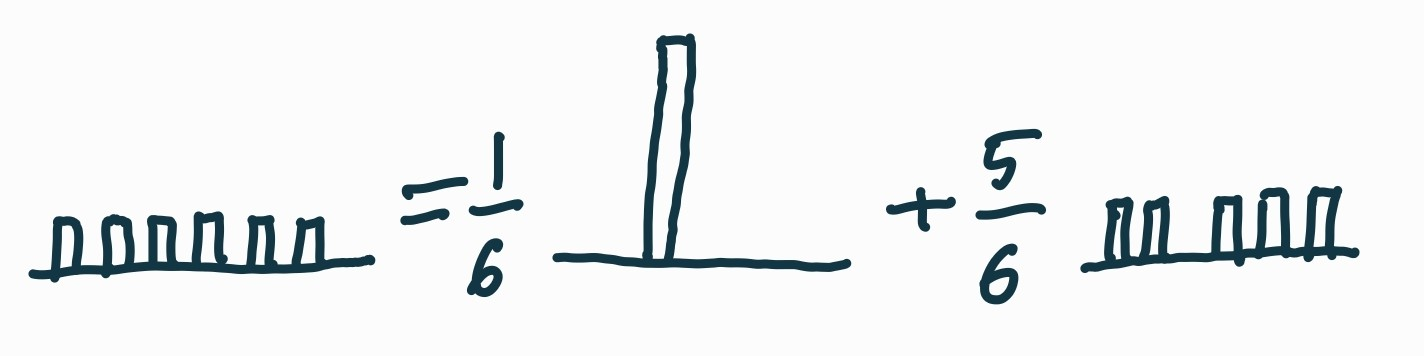
\includegraphics[width=0.6\textwidth]{tempimages/Fraction.jpg}
\end{figure}

First we define the \textbf{fraction} of one element within another. For example, suppose $\ens_{123456}$ is a uniform distribution for a six-faced die. Suppose $\ens_3$ represents the outcome 3 with $100\%$ probability. Then $\ens$ can be understood as $\ens_{123456} = \frac{1}{6} \ens_3 + \frac{5}{6} \ens_{12456}$ where $\ens_{12456}$ is the uniform distribution over the outcomes 1,2,4,5 and 6. Note that $\frac{1}{6}$ is the highest coefficient we can put in front of $\ens_3$ in a convex combination and have $\ens_{123456}$ as a result, which coincides with the probability of obtaining 3 from a uniform distribution over six outcomes. That is what we define the fraction of $\ens_3$ in $\ens_{123456}$ to be.

\begin{mathSection}
	\begin{defn}
		Let $\ens, \ens[a] \in \Ens$ be two ensembles. The \textbf{fraction} of $\ens[a]$ in $\ens$ is the greatest mixing coefficient for which $\ens$ can be expressed as a mixture of $\ens[a]$. That is, $\size_{\ens}(\ens[a]) = \sup(\{ p \in [0,1] \, | \, \exists \, \ens[b] \in \Ens \text{ s.t. }  \ens = p \ens[a] + \bar{p} \ens[b] \})$.
	\end{defn}
\begin{figure}[H]
	\centering
	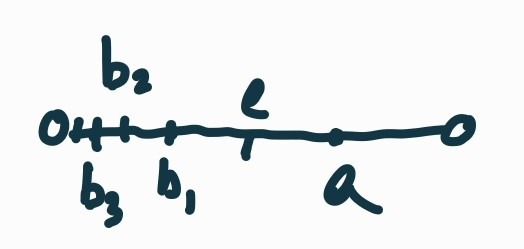
\includegraphics[width=0.4\textwidth]{tempimages/CapacitySupremum.jpg}
\end{figure}
	
	\begin{remark}
		We need to take the supremum as the maximum may not exist. For example, consider a discrete classical ensemble space and remove the extreme points. At the moment, there is no reason to rule out such space as unphysical.
	\end{remark}
	
	\begin{coro}
		Let $\ens, \ens[a] \in \Ens$, then $\size_{\ens}(\ens[a]) = 0$ if and only if $\ens[a]$ is not a component of $\ens$.
	\end{coro}
	
	\begin{proof}
		Note that $\ens[a]$ is a component of $\ens$ if we can write $\ens = \lambda \ens[a] + \bar{\lambda} \ens[b]$ for some $\lambda \in (0,1]$ and $\ens[b] \in \Ens$. In this case, $\size_{\ens}(\ens[a]) \geq \lambda > 0$. Conversely, if $\size_{\ens}(\ens[a]) > 0$ we can find $\size_{\ens}(\ens[a]) \geq \lambda > 0$ such that $\ens = \lambda \ens[a] + \bar{\lambda} \ens[b]$ for some $\ens[b] \in \Ens$.
	\end{proof}
\end{mathSection}

Intuitively, we would expect the following conjecture to be true:
\begin{conj}
	The fraction capacity $\fcap_{\ens}(\ens[a])$ is a continuous function both in $\ens[a]$ and $\ens$.
\end{conj}


\begin{figure}[h]
	\centering
	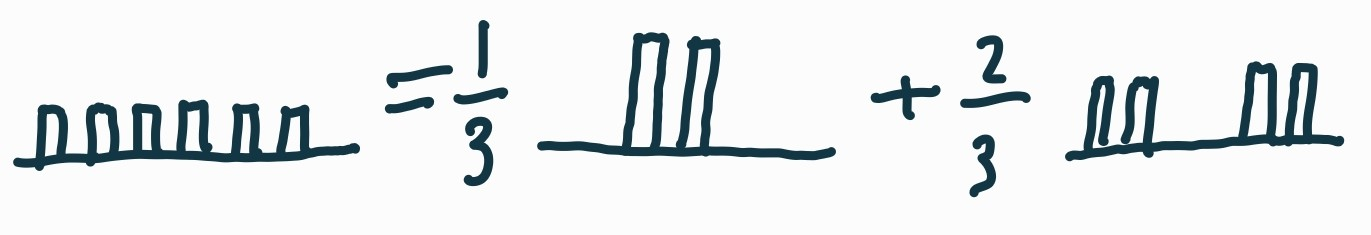
\includegraphics[width=0.6\textwidth]{tempimages/FractionCapacity.jpg}
\end{figure}

We now define \textbf{fraction capacity} of a set of ensembles for another ensemble. Like before, suppose $\ens_{123456}$ is a uniform distribution for a six-faced die, but now take $A = \{ \ens_3, \ens_4 \}$ as, respectively, the outcomes $3$ and $4$ with $100\%$ probability. Then $\ens$ can be understood as $\ens_{123456} = \frac{1}{3} \left(\frac{1}{2} \ens_3 + \frac{1}{2} \ens_4 \right) + \frac{2}{3} \ens_{1256}$, where $\ens_{1256}$ is the uniform distribution over outcomes 1,2,5 and 6. Again, note that $\frac{1}{3}$ is the highest coefficient we can put in front of any convex combinations of elements of $A$, and still make a convex combination that has $\ens$ as a result. That is what we define the fraction capacity of $A$ for $\ens_{123456}$ to be.

The fraction capacity, then, defines how much of the ensemble $\ens$ can be constructed with elements of $A$. The term capacity is used first because, intuitively, it tells us how much $A$ can hold, and second because capacity is a name used to describe non-additive measures. The fraction capacity, in fact, has several nice properties. First, its value is always between zero and one, since the coefficient of a convex combination must be so bound. Second, it is monotone in the sense that if $A$ gets bigger, the fraction capacity cannot decrease. Third, it is subadditive, meaning that the fraction capacity of the union of two sets must be the sum of the respective fraction capacities or less. Fourth, it is continuous. Note that if subadditivity is replaced by additivity, these are exactly the defining properties of a probability measure, since additivity and continuity are equivalent to $\sigma$-additivity.

\begin{mathSection}
	\begin{defn}
		Let $\ens \in \Ens$ be an ensemble and $A \subseteq \Ens$ a Borel set. The \textbf{fraction capacity} of $A$ for $\ens$ is the biggest fraction achievable with convex combinations of $A$. That is, $\fcap_{\ens}(A) = \sup(\size_{\ens}(\hull(A))\cup\{0\})$.
	\end{defn}
	
	\begin{remark}
		An open question is whether the type of hull matters.
	\end{remark}

	\begin{coro}
		The fraction capacity uniquely identifies an ensemble. That is, let $\ens[a], \ens[b] \in \Ens$ such that $\ens[a] \neq \ens[b]$. Then $\fcap_{\ens[a]} \neq \fcap_{\ens[b]}$.
	\end{coro}
	
	\begin{proof}
		Note that $\ens = 1 \ens[a] + 0 \ens[b]$ if and only if $\ens = \ens[a]$. Therefore, let $\ens[a], \ens[b] \in \Ens$ such that $\ens[a] \neq \ens[b]$. We have $\fcap_{\ens[a]}(\{\ens[a]\}) = 1$ and $\fcap_{\ens[b]}(\{\ens[a]\}) \neq 1$. Which means $\fcap_{\ens[a]} \neq \fcap_{\ens[b]}$.
	\end{proof}
	
	\begin{prop}
		The fraction capacity for an ensemble is a set function that is
		\begin{enumerate}
			\item non-negative and unit bounded: $\fcap_{\ens}(A) \in [0,1]$
			\item monotone: $A \subseteq B \implies \fcap_{\ens}(A) \leq \fcap_{\ens}(B)$
			\item subadditive: $\fcap_{\ens}(A \cup B) \leq \fcap_{\ens}(A) + \fcap_{\ens}(B)$
			\item continuous from below: $\fcap_{\ens}(\lim\limits_{i \to \infty} A_i) = \lim\limits_{i \to \infty} \fcap_{\ens}(A_i)$ for any increasing sequence $\{A_i\}$
			\item continuous from above: $\fcap_{\ens}(\lim\limits_{i \to \infty} A_i) = \lim\limits_{i \to \infty} \fcap_{\ens}(A_i)$ for any decreasing sequence $\{A_i\}$
		\end{enumerate}
	\end{prop}
	
	\begin{proof}
		1. The fraction capacity takes a subset of $\Ens$ and returns a real value and is therefore a set function. The mixture coefficients are real values between zero and one. The supremum of a set of numbers between zero and one is between zero and one, and therefore the fraction capacity for an ensemble is non-negative and unit bounded.
		
		2. The $\hull$ is a monotone function. The image of a set through a map is a monotone function. The supremum is a monotone function. Therefore the fraction capacity is a monotone function.
		
		3. Let $A, B \subseteq \Ens$ and let $p \in [0,1]$ such that $\ens = p \ens_1 + \bar{p} \ens_2$ for some $\ens_1 \in \hull(A \cup B)$ and $\ens_2 \in \Ens$. Since $\ens_1 \in \hull(A \cup B)$, we can write $\ens_1 = \lambda \ens[a] + \bar{\lambda} \ens[b]$ for some $\lambda \in [0,1]$, $\ens[a] \in A$ and $\ens[b] \in B$. Therefore we have $\ens = p \lambda \ens[a] + p \bar{\lambda} \ens[b] + \bar{p} \ens_2$. By the definition of fraction capacity, we must have $p\lambda \leq \fcap_{\ens}(A)$ and $p\bar{\lambda} \leq \fcap_{\ens}(B)$, therefore $p = p\lambda + p\bar{\lambda} \leq \fcap_{\ens}(A) + \fcap_{\ens}(B)$. 	Since $\fcap_{\ens}(A \cup B)$ is the supremum for a set of $p$s for which the expression always holds, we have $\fcap_{\ens}(A \cup B) \leq \fcap_{\ens}(A) + \fcap_{\ens}(B)$. The fraction capacity is subadditive.
		
		4. Let $\{A_i\} \subseteq \Sigma_{\Ens}$ be an increasing sequence. That is $A_i \subseteq A_{i+1}$ for all $i$. Given that the fraction capacity is monotone, $\{\fcap_{\ens}(A_i)\}$ is an increasing sequence. Note that $\fcap_{\ens}(A_i) \leq 1$ for all $i$, therefore the sequence will have an upper bound which will coincide with the limit. Let $A = \lim\limits_{i \to \infty} A_i$. We have $A = \bigcup A_i$ and $A_i \subseteq A$ for all $i$. Since fraction capacity is monotone, we have $\fcap_{\ens}(A_i) \leq \fcap_{\ens}(A)$ for all $i$ and therefore $\lim\limits_{i \to \infty} \fcap_{\ens}(A_i) \leq \fcap_{\ens}(A)$. Suppose $\lim\limits_{i \to \infty} \fcap_{\ens}(A_i) < \fcap_{\ens}(A)$. Then there would be an $\ens[a] \in \hull(A)$ such that $\size_{\ens}(\ens[a]) > \size_{\ens}(\ens[b])$ for all $\ens[b] \in \hull(A_i)$ for all $i$. But if $\ens[a] \in \hull(A)$, then it can be written as a finite combination of finitely many elements of $A$. Then we will be able to find a $k$ such that $A_k$ will contain all the elements, and therefore $\ens[a] \in A_k$. But this means $\ens[a] \leq \fcap_{\ens}(A_k)$ which is a contradiction. Therefore $\lim\limits_{i \to \infty} \fcap_{\ens}(A_i) = \fcap_{\ens}(A)$.
		
		5. The previous argument works in the same way for decreasing sequences by inverting the order.
	\end{proof}
\end{mathSection}

\begin{conj}
	The fraction capacity $\fcap_{\ens}$ is additive over $A, B \subseteq \Ens$ if and only if there exists a $C \subseteq \Ens$ such that $A \separate B$, $B \separate C$, $A \separate C$ and $\ens \in \hull(A\cup B\cup C)$.
\end{conj}

\begin{conj}
	The fraction capacity is $\sigma$-subadditive. That is, $\fcap_{\ens}(\bigcup A_i) \leq \sum_i \fcap_{\ens}(A_i)$.
\end{conj}

\begin{remark}
	In \href{https://link.springer.com/book/10.1007/978-3-319-30690-2}{Set Functions, Games and Capacities in Decision Making}, it is claimed that finite additivity plus continuity implies $\sigma$-additivity. The conjecture is that this generalizes to $\sigma$-subadditivity.
\end{remark}

We now show that fraction capacity recovers classical probability in the classical case. The key insight is that each event, each Borel set $A$, corresponds to a subspace of probability measures for which that event will be true. This is the set of probability measure whose support is always within the given Borel set $A$. A probability measure, then, can always be decomposed in a part for which that event will be true, the part supported by $A$, and a part for which that event will be false, the part supported by the complement. The fraction capacity correspond to the mixing coefficient of this decomposition.
\begin{mathSection}
	\begin{prop}
		Let $\Ens$ be a discrete or continuous classical ensemble space with sample space $X$. Let $A \in \Sigma_X$ be an event and $\Ens_A \subseteq \Ens$ the set of distributions with support contained in $A$. Let $p \in Ens$ a probability measure in the ensemble space. Then $p(A) = \fcap_{p}(\Ens_A)$. That is, the probability of an event is equal to the fraction capacity of the subspace corresponding to that event.
	\end{prop}
	\begin{proof}
		Let $p \in \Ens$ be a probability measure over $X$, absolutely continuous with respect to the appropriate measure $\mu$ (i.e. discrete for discrete case and Liouville for continuous case). Given $A \in \Sigma$, we can write $p = p(A) p_A + p(A^{\complement}) p_{A^{\complement}}$ where  $p_A$ is a probability measure with support $A$ and $p_{A^{\complement}}$ is a probability measure with support to $A^{\complement}$.
		
		Let $\Ens_A \subseteq \Ens$ be the subset of probability measures with support contained in $A$. Then $p_A \in \Ens_A$ and $\fcap_{p}(\Ens_A) \geq p(A)$. Given that $p_{A^{\complement}}$ has support disjoint from $A$, we can find no further component of $p$ that has support in $A$. Therefore $\fcap_{p}(\Ens_A) = p(A)$. The fraction capacity, then, recovers the probability.
	\end{proof}
\end{mathSection}
	
We now show that the fraction capacity recovers probability over measurements in the quantum case. The setup is essentially the same as of the classical case, except that we start with an observable $O$, and each Borel set $A$ for that observable will have a corresponding subspace of $\mathcal{H}$ and a projector $\Pi_A$. A post-measurement state of $O$ is mixed state that commutes with $O$, since it will commute with any projector that commutes with $O$. We can show, then, that the fraction capacity recovers the decomposition of any post-measurement state of $O$ over the subspace corresponding to $\Pi_A$.

\begin{mathSection}
	\begin{prop}
		Let $\Ens$ be a quantum ensemble space associated to a Hilbert space $\mathcal{H}$. Let $O : \mathcal{H} \to \mathcal{H}$ be a quantum observable. Let $A \in \Sigma_{\mathbb{R}}$ be a Borel set and $\Pi_{A}$ be the projection associated with the subspace of $\mathcal{H}$ corresponding to the subset $A$ of the spectrum of $O$. Let $\Ens_A$ be the set of ensembles within that subspace. Let $\rho \in \Ens$ be a mixed state that commutes with $O$ (i.e. the ensemble resulting form a measurement of $O$). Then $\tr(\rho \Pi_A) = \fcap_{\rho}(\Ens_A)$.
	\end{prop}
	
	\begin{proof}
		Let $\rho \in \Ens$ be a mixed state that commutes with $O$. Let $A \in \Sigma_{\mathbb{R}}$ be a Borel set and $\Pi_{A}$ be the projection associated with the subspace of $\mathcal{H}$ corresponding to the subset $A$ of the spectrum of $O$. Then we can write $\rho = \lambda \rho_A + \bar{\lambda} \rho_{A^{\complement}}$ where $\rho_A, \rho_{A^{\complement}} \in \Ens$ are such that $\tr(\rho_A \Pi_A) = 1$ and  $\tr(\rho_{A^{\complement}} \Pi_A) = 0$. We have $\tr(\rho \Pi_A) = \lambda$.
		
		Let $\Ens_A \subseteq \Ens$ be the subset of mixed states $d$ such that $\tr(d \Pi_A) = 1$. Then $d \in \Ens_A$ and $\fcap_{\rho}(\Ens_A) \geq \lambda$. Given that $\rho_{A^{\complement}}$ is in the subspace orthogonal to $\Ens_A$, we can find no further component of $\rho$ in that subspace. Therefore $\fcap_{p}(\Ens_A) = \lambda$. We have $\tr(\rho \Pi_A) = \lambda = \fcap_{p}(\Ens_A)$ The fraction capacity, then, recovers the probability.
	\end{proof}
\end{mathSection}

\section{Statistical properties and quantities}

In this section we define statistical quantities, which are the generalization of classical random variables and quantum observables. Given our ensembles first approach, statistical quantities are affine (linear) functions of ensembles as they represent an expectation over ensembles. The possible values of the quantities will need to be recovered with constructions that mimic spectral theory, though we will not want to talk about eigenstates and eigenvalues in the general case since these are not properly defined for a continuous quantity.

\subsection{Properties and quantities}

These definitions extend the notion of properties and quantities that we defined for an experimental domain. In that case, we simply required that a property be a continuous map to a set of possible values for the property. For a statistical property, the set of values are a topological convex space, so that the property allows statistical mixing. For a quantity, the topological convex space is simply a linearly ordered property, which in this case will always be a real valued quantity. The convexity, the averaging operation, fills in the gaps in the linear order in case that not all intermediate values can be obtained.

\begin{mathSection}
	
\begin{defn}
	A \textbf{statistical property}, or simply property, is an attribute that allows statistical mixing. Formally, it is an continuous map $F : \Ens \to \mathcal{Q}$ where $\mathcal{Q}$ is a convex topological space such that $F(p \ens[a] + \bar{p} \ens[b]) = p F(\ens[a]) + \bar{p} F(\ens[b])$ (i.e. it is an affine map).
	
	A \textbf{statistical quantity}, or statistical variable, or simply variable, is a numerical statistical property. That is, it is a continuous linear real valued operator $F : \Ens \to \mathbb{R}$.
\end{defn}

\begin{justification}
	This definition extends the general definition of properties and quantities we already gave to the statistical case. As before, continuity is required since verifying the value of the quantity corresponds to verifying that we are dealing with a specific subset of ensembles.
	
	The ability to create convex combinations corresponds to the ability to create statistical averages. Therefore $\mathcal{Q}$ must be a convex set. Given that preparation instances are assumed to be independent, a mixture of the preparation will produce a mixture of the properties according to the same fraction coefficients.
	
	Quantities are simply properties that are linearly ordered. The ability to create convex combinations becomes the ability to take weighted averages of the quantities. Regardless of whether one starts from integers, rationals or real valued quantities, the statistical averages will, in general, be a real number.
	
	Note that the numerical value cannot be infinite. The only way to measure infinity is if the measured average keeps increasing in time. This would be a contradiction on the assumption that the ensemble represent a reproducible collection of preparations.
\end{justification}

\begin{remark}
	Note that variables will have a contiguous range on the ensembles because, given two ensembles with different values, we can mix them to obtain any intermediate value. This does not mean that the variable can take all possible values on pure states. For example, the number of particles in a pure state will necessarily be a non-negative integer, but we can mix those to create ensembles that have non-integer average number of particles.
\end{remark}

\begin{coro}
	A set of statistical quantities $\{F_i\}_{i \in I}$ can be collected into a single statistical property $F : \Ens \to \mathbb{R}^I$ where $F(\ens) = \{F_i(\ens)\}_{i \in I}$.
\end{coro}
\end{mathSection}

Here we show that statistical quantities recover the standard random variables of classical mechanics. That is, every statistical variable is a random variable and every random variable is a statistical variable.

\begin{mathSection}
\begin{prop}
	Let $\Ens$ be a classical probability space. Then each statistical quantity is the expectation of a random variable and vice-versa.
\end{prop}

\begin{proof}
	Let $\Ens$ be an ensemble space where each ensemble is a probability measure $\mu$ over some sample space $X$. Let $f : X \to \mathbb{R}$ be a random variable, then the expectation $F(\mu) \mapsto \int_{X} f d\mu$ is a continuous real affine map and is therefore a statistical quantity. Conversely, let $F : \Ens \to \mathbb{R}$ be a linear functional of the measures. Then, by Riesz representation theorem, we can write $F(\mu) = \int_{X} f d\mu$ from some $f : X \to \mathbb{R}$.
\end{proof}
\end{mathSection}

For a quantum system, we can show that all expectations of observables are statistical quantities.

\begin{mathSection}
\begin{prop}
	Let $\Ens$ be a quantum ensemble space. All expectations of observables are statistical quantities.
\end{prop}

\begin{proof}
	Let $\Ens$ be a quantum ensemble space over some Hilbert space $\mathcal{H}$. Let $O : \mathcal{H} \to \mathcal{H}$ be Hermitian operator. Then $F(\rho) \mapsto \tr(\rho O)$ is a continuous real affine map of $\Ens$ and it is therefore a statistical quantity.
\end{proof}

\begin{remark}
	We still need to prove that the converse is true: every statistical quantity in quantum mechanics corresponds to an operator. We may need to constrain the problem to bounded quantities, and recover the unbounded only as a limit.
\end{remark}
\end{mathSection}


\subsection{Quantifiable spaces and locally convex vector spaces}

In physics, we typically are able to fully identify ensembles by using measurable quantities. An ensemble space is quantifiable, then, when we have enough statistical quantities to recover all ensemble. There is a subtle problem with infinity, though, that is still not completely closed.

In principle, the space of ensemble may include quantities whose expectation is infinite over some distributions. In classical mechanics, for example, given any probability distribution $\rho$ with infinite support we can find a random variable $f$ such that $\int_X f \rho dx$ diverges. For example, we can simply set $f(x) = 1/\rho(x)$ where $\rho(x)\neq0$ and $\rho(x) = 0$ otherwise. This can be solved in classical mechanics because we can always find distributions with compact support, which will guarantee convergence for all functions. In quantum mechanics, however, a wavefunction with compact support on position will have non-compact support in momentum and vice-versa. However, the Schwartz wavefunctions will have finite expectation for all polynomial of position and momentum, and they are dense in the Hilbert space. What makes sense to expect physically, then, is that there is a set of quantities that physically define the system which will need finite expectation. These will need to remain finite under coordinate transformations and time evolution for the physics to make sense. All these details are yet to be understood and framed in a mathematically precise way. Yet, it is clear that we need, at least, to characterize the case where a set of statistical quantities fully characterize all ensembles.

\begin{defn}
	A \textbf{quantifiable} ensemble space is an ensemble space where each ensemble can be identified by a set of statistical variables. That is, there is family of statistical variables $F_i : \Ens \to \mathbb{R}$ such that, given $\ens_1, \ens_2 \in \Ens$, $F_i(\ens_1) = F_i(\ens_2)$ for all $i$ if and only if $\ens_1 = \ens_2$. Moreover, the topology is generated by those variables.
\end{defn}

We are going to show that the statistical variables can be used to construct semi-norms on the embedding vector space inducing a topology that is Hausdorff and locally convex. Since the statistical variables are continuous in both the topology of the ensemble space and on this topology of the embedding vector space, the embedding of the ensemble space is continuous. Note that this embedding is not necessarily a homeomorphism onto the image as convergence on the expectation of continuous variables (i.e. weak convergence) does not guarantee converge of the entropy (which requires converges through the inner product).

\begin{prop}
	A statistical variable $F$ induces a semi-norm on the vector space that embeds $\Ens$.
\end{prop}

\begin{proof}
	Let $F$ be a variable on $\Ens$, let $\ens[a] \in \Ens$ an internal point and let $V_{\ens[a]}$ be the vector space of differences. Define $F_{\ens[a]} : V_{\ens[a]} \to \mathbb{R}$ such that $F_{\ens[a]}([r(\ens[b]-\ens[a])]) = |r (F(\ens[b]) - F(\ens[a]))|$.
	
	First we show that $F_{\ens[a]}$ does not depend on the representative. If we have the zero class, then either $r=0$ or $\ens[b] = \ens[a]$. In both cases, the function evaluates to zero. For the non-zero class, we have
	\begin{equation}
		\begin{aligned}
			F_{\ens[a]}\left(\left\{(r+j)\left(\left(\frac{r}{r+j}\ens[b] +\frac{j}{r+j} \ens[a]\right) -\ens[a]\right)\right\}\right) &= \left\{ \left|(r+j)\left(F\left(\frac{r}{r+j}\ens[b] +\frac{j}{r+j} \ens[a]\right) - F(\ens[a]) \right)\right| \right\} \\
			&= \left\{ \left|(r+j)\left(\frac{r}{r+j}F(\ens[b]) +\frac{j}{r+j} F(\ens[a]) - F(\ens[a]) \right)\right| \right\} \\
			&= \left\{ \left| r F(\ens[b]) + j F(\ens[a]) - (r+j) F(\ens[a]) \right| \right\} \\
			&= \left\{|r (F(\ens[b]) - F(\ens[a]))|\right\}.
		\end{aligned}
	\end{equation}
	
	Since $F_{\ens[a]}$ evaluates to an absolute value, it is a non-negative function. Since $F_{\ens[a]}(r[s(\ens[b]-\ens[a])]) = F_{\ens[a]}([(rs)(\ens[b]-\ens[a])]) = |(rs) (F(\ens[b]) - F(\ens[a]))| = |r| |s (F(\ens[b]) - F(\ens[a]))| = |r| F_{\ens[a]}([s(\ens[b]-\ens[a])])$, $F_{\ens[a]}$ is absolutely homogeneous. We also have
	\begin{equation}
	\begin{aligned}
		&F_{\ens[a]}([r(\ens[b]-\ens[a])] + [s(\ens[c]-\ens[a])])  \\
		&= F_{\ens[a]}\left(\left[(r+s+k) \left(\left(\frac{r}{r+s+k}\ens[b] + \frac{s}{r+s+k} \ens[c] +\frac{k}{\alpha r+ \beta s+k} \ens[a] \right) - \ens[a]\right)\right]\right) \\
		&= \left|(r+s+k)\left(F\left(\frac{r}{r+s+k}\ens[b] + \frac{s}{r+s+k} \ens[c] +\frac{k}{r+s+k} \ens[a]\right) - F(\ens[a]) \right)\right| \\
		&= \left|r F(\ens[b]) + s F(\ens[c]) + k F(\ens[a]) - (r+s+k) F(\ens[a]) \right| \\
		&= \left|r ( F(\ens[b]) - F(\ens[a]))  + s ( F(\ens[c]) - F(\ens[a])) \right| \\
		&\leq \left| r ( F(\ens[b]) - F(\ens[a])) \right| + \left| s ( F(\ens[c]) - F(\ens[a])) \right| \\
		&= F_{\ens[a]}([r(\ens[b]-\ens[a])]) + F_{\ens[a]}([s(\ens[c]-\ens[a])]).
	\end{aligned}
	\end{equation}
	This means that $F_{\ens[a]}$ is sub-additive. Therefore $F_{\ens[a]}$ is a seminorm by \href{https://en.wikipedia.org/wiki/Seminorm}{definition}.
\end{proof}

\begin{prop}
	A quantifiable ensemble space embeds continuously into a Hausdorff locally convex topological vector space.
\end{prop}

\begin{proof}
	Let $\Ens$ be a quantifiable ensemble space and $V_{\ens[a]}$ be the embedding vector space corresponding the the internal point $\ens[a] \in \Ens$. Consider all the semi-norms defined by the family of statistical variables that make $\Ens$ quantifiable. These will induce a topology on $V_{\ens[a]}$ making it a topological vector space (see \href{https://personal.math.ubc.ca/~cass/research/pdf/TVS.pdf}{Prop 2.2 in here}). Since the topology is generated by semi-norms, it is locally convex. Since the semi-norms fully identify each point, the topology is Hausdorff (see \href{https://personal.math.ubc.ca/~cass/research/pdf/TVS.pdf}{Prop 2.6 in here}).
	
	Now consider $\Ens$ as embedded into $V_{\ens[a]}$. If $F : \Ens \to \mathbb{R}$ is a statistical variable, then $|r F(\ens[b]) - F(\ens[a]) |$ is also a statistical variable since difference, scalar multiplication and absolute value are all continuous. This means that the open ball given by the semi-norm on the vector space restricted to the ensemble space are the open sets as they correspond to the open balls in the ensemble space. Moreover, since $F_i$ are continuous in the ensemble space, a convergent sequence in the ensemble space will correspond to the convergence of all the semi-norms in the vector space, thus convergence in the topology generated by said semi-norms. The embedding, then, is continuous.
\end{proof}

At this point, we are not guaranteed that ensembles can be characterized by a countable family of statistical variables. The issue is that, while a second countable locally convex topology is generated by countably many semi-norms, we know that the topology of the ensemble space is second countable but we do not know whether the subtopology generated by the statistical variables through the semi-norms is second countable. Physically, it would mean that we have a way to experimentally distinguish between two ensembles (i.e. a second countable topology) but not through the expectation of statistical quantities. The entropy would, for example, provide other more stringent ways. It is not yet clear whether this is something that can indeed happen, and therefore a potential source of new physics, or we simply are missing a way to prove the result. Currently, the second option seems more likely.

If one is able to prove that the topology induced by the statistical variables is second countable, or if we simply impose that a countable family of statistical variables is enough to distinguish between ensembles, then the space is a metrizable second countable locally convex topological vector space.

\begin{prop}
	If a quantifiable ensemble spaces is fully determined by countably many statistical variables, then it embeds continuously into a metrizable second countable locally convex topological vector space.
\end{prop}

\begin{proof}
	If a quantifiable ensemble space is characterized by countably many statistical variables, the topology induces on the vector space is second countable. A Hausdorff second countable topological vector space is metrizable.
\end{proof}

\begin{remark}
	Note that we are missing completeness in terms of the semi-norms to obtain a Fr\'echet space and it is unclear we are going to have it. For the classical case, suppose we restrict ourselves to all absolutely continuous probability measures with compact support. Expectation of all polynomials of position and momentum fully identify the measure. However, Dirac measures are also fully identified by those quantities, which can be achieved as the limit of a uniform distribution whose support shrinks to a point. That would give us a sequence of convergent expectation whose ensemble does not converge in the space.
\end{remark}

\begin{prop}
	Discrete/continuous classical ensemble spaces and quantum ensemble spaces are quantifiable.
\end{prop}

\begin{proof}
	For discrete classical spaces, the expectation of the indicator of each extreme point defines a countable set of quantities that fully identifies the distribution.
	
	For continuous classical spaces, note that $L^1(\mathbb{R}^{2n})$ is a Hausdorff locally convex topological spaces.
	
	For quantum ensemble spaces, the expectation of projectors define a family of statistical variables that can distinguish any pair of mixed states.
\end{proof}

An open problem is whether statistical quantities are required by ensemble spaces or they are an additional requirement. If we were able to show that ensemble spaces always embed continuously in a locally convex topological vector space, one may use the semi-norms to define quantities. Another approach is to investigate whether the existence of linear transformations parameterized by real quantities give us statistical quantities through the generators of the transformations. Physically, this would correspond to the assumption that time is a continuous quantity. It would also mean that, if time is not modeled as a real quantity, then the ensemble space would have to change.

\subsection{Connection to Choquet theory}

We now connect ensemble spaces to Choquet theory. Given a compact convex subset $E$ of a locally convex topological vector space $V$, Choquet theory asks whether every point of $E$ can be represented as a probability measure over its extreme points. If an ensemble space $\Ens$ is compact, or allows a completion completion $E$, then we can study the ensemble space within Choquet theory as well. The fraction capacity can be understood as the supremum from all measures that can represent an ensemble. The fraction capacity is therefore additive only if all ensembles can be represented with only one measure (i.e. multiple decomposition is not allowed).

Choquet theory can be summarized in the following way. First, we need to define what it means to represent an ensemble with a probability measure. Let $E$ be a convex subset of a locally convex topological vector space $V$ and $X$ the set of extreme points. We say that $\ens \in E$ is represented by a probability measure $p : \Sigma_{E} \to [0,1]$ if $F(\ens) = \int_E F dp$ for every continuous linear functional $F$ on $V$. Moreover, we say that $p$ is supported by the extreme points if $p(X) = 1$. Given any probability measure $p$ over the extreme points $X$, we can always find an $\ens \in E$ that is represented by $p$. Therefore, we have a map from the set of probability measures to the set of ensembles. Choquet theory characterizes how the map works in the opposite direction.

The first question is whether each ensemble is represented by a probability measure. Choquet theory tells us that this is the case:
\begin{thrm}[Choquet-Bishop-de Leeuw]
	Let $E$ be a compact convex subset of a locally convex topological vector space $V$, and let $\ens \in E$. Then there exists a probability measure $p_{\ens}$ on $X$ which represents $\ens$ and is supported by the extreme points $X$.
\end{thrm}
The second question is whether the representation is unique. Choquet theory has a clear answer.
\begin{thrm}[Choquet uniqueness]
	Let $E$ be a compact convex subset of a locally convex topological vector space $V$. Then $E$ is a Choquet simplex if and only if for each $\ens \in E$ there exists a unique measure $p_{\ens}$ which represents $\ens$ and is supported by the extreme points $X$.
\end{thrm}
The definition of a Choquet simplex is rather involved, so it is omitted. Intuitively, it is the generalization of the finite dimensional simplex and we can take is a definition. The key point is that $E$ is a Choquet simplex if and only if the ensemble space does not allow multiple decompositions in terms of extreme points.

There is a connection between mixtures and the representation through a probability measure. We can, in fact, write $\ens = \lambda \ens[a] + \bar{\lambda} \ens[b]$ if and only if $\ens$ can be represented by the probability measure $p(\{\ens[a]\}) = \lambda$, $p(\{\ens[b]\}) = \bar{\lambda}$, and $p(\Ens \setminus \{\ens[a], \ens[b]\}) = 0$. Therefore, if $M_{\ens}$ is the set of probability measre that represent $\ens$, the fraction $\size_{\ens}(\ens[a])$ is given by the maximum value over $\{\ens[a]\}$ that can be taken by one of those measures. That is,  $\size_{\ens}(\ens[a]) = \sup \{ p(\{\ens[a]\}) \, | \, M_{\ens} \}$.

\begin{prop}
	Let $E$ be a compact convex subset of a locally convex topological vector space $V$ and define the fraction capacity as for an ensemble space. Let $\ens \in E$ be a point and $M_{\ens}$ be the set of measures that represent $\ens$. Then $\size_{\ens}(\ens[a]) = \sup \{ p(\{\ens[a]\}) \, | \, M_{\ens} \}$ and $\fcap_{\ens}(A) = \sup \{ p(\{A\}) \, | \, M_{\ens} \}$.
\end{prop}

\begin{proof}
	Let $\ens \in E$ and suppose $\ens = \lambda \ens[a] + \bar{\lambda} \ens[b]$ with $\ens[a], \ens[b] \in E$ and $\lambda \in [0,1]$. The measure $p$ such that $p(\{\ens[a]\}) = \lambda$, $p(\{\ens[b]\}) = \bar{\lambda}$ and $p(E\setminus \{ \ens[a], \ens[b]\})=0$ represents $\ens$. The converse is true as well. Therefore $\size_{\ens}(\ens[a]) = \sup \{ p(\{\ens[a]\}) \, | \, M_{\ens} \}$. 
\end{proof}


In case $E$ is compact, we can restrict the fraction capacity to the set $X$ of extreme points. Given a set $A \subset X$, of extreme points, we can find the set $N \subset E$ of all ensembles that can be represented with a probability measure with support $A$. This forms a convex set. Now, the ability to express an ensemble $\ens$ as the convex combination of $N$ is precisely the ability to find a measure $p$ that represents $\ens$ such that $p(A) \neq 0$. That is, $\ens = \lambda \ens[a] + \bar{\lambda} \ens[b]$ with $\ens[a] \in M$ if and only if there is a probability measure $p$ that represents $\ens$ such that $p(A) \geq \lambda$.\footnote{TODO: add proof somewhere} Consequently, if $M_{\ens}$ is the set of all probability measures that represent $\ens$ as defined in Choquet theory, then $\fcap_{\ens}(A) = \sup(\{p(A) \, | \, p \in M_{\ens}\})$.\footnote{TODO: prove somewhere} The fraction capacity is simply the supremum on each set over all possible measures.

\begin{prop}
	Let $E$ be a compact convex The following statements are equivalent:
	\begin{enumerate}
		\item $\Ens$ is a Choquet simplex
		\item each ensemble is uniquely represented by a measure over its extreme points $X_{\Ens}$
		\item the fraction capacity restricted over the extreme points is additive
	\end{enumerate}
	
	An ensemble space $\Ens$ is a Choquet simplex if an only if Let $E$ be a closed convex metrizable subset of a locally convex topological vector space $V$. Then $E$ is a Choquet simplex if and only if for each $\ens \in E$ there exists a unique measure $p_{\ens}$ which represents $\ens$ and is supported by the extreme points $X$.
\end{prop}


\subsection{Macrostates and thermodynamics}

In this section we try to recover some elements of thermodynamics on the generalized ensemble space. We want to recover Gibbs' thermodynamics, which means an equation of state in terms of extensive quantities. Instead of extensive quantities, we are going to use statistical quantities. Note that the idea that all extensive quantities are statistical (i.e. the average during mixing) seems to work. The energy and the number or particles average during mixture. The idea that volume averages during mixture can be understood as the system oscillating between the different volumes defined by the components. It also seems that intensive quantities do not average during mixing. Temperature, for example, is only defined on equilibria (i.e. of Boltzmann distributions) and the mixture of two equilibria at different temperature is not an equilibrium. Still, we would need a general proof, which would require the notion of product spaces (i.e. intensitive/extensive quantities represent system/subsystem relationship).

\begin{defn}
	Let $\Ens$ be an ensemble space. Let $F : \Ens \to \mathcal{Q}$ be a statistical property. The \textbf{coarse graining} of $\Ens$ over $F$ is the set $\mathcal{M} \subseteq \Ens$ represented by the ensemble that maximize the entropy for each fixed value of the property. That is, there exists a map $\psi : \mathcal{Q} \to \mathcal{M}$ such that $F(\psi(x)) = x$ and $S(\psi(x)) \geq \ens$ for all $\ens \in \Ens$ such that $F(\ens) = x$. The \textbf{equation of state} is the map $S(x) \mapsto S(\psi(x))$ that returns the entropy given the value of the statistical property.
\end{defn}

The set of ensemble that maximize entropy will be a set of points fully identified by finitely many real numbers. We would expect this to be a manifold, though we still have to understand how the topology of the ensemble space related to the topology of $\mathcal{M}$.

\begin{conj}
	Let $F : \Ens \to \mathbb{R}^n$ be a vector of statistical quantities. Then the corresponding coarse graining of $\mathcal{M}$ is a manifold. The equation of state $S : \mathbb{R}^n \to \mathbb{R}$ returns the entropy as a function of the statistical values.
\end{conj}

\begin{remark}
	We need to prove that $\mathcal{M}$ inherits the topology from $\Ens$. Are we be able to recover the topological isolation of phase transitions? The quantities will typically be energy plus other extensive quantities (i.e. volume, number of particles, ...).
\end{remark}

What can we already prove, however, is that the entropy is a strictly concave function of the state variables. Note that, in this setting, the convex combination between state variables does not give a statistical mixture, but rather it give us the ensemble that maximizes entropy on the averaged constrain. Therefore, the concavity of the entropy on the coarse grained state is not the same concavity of the entropy on the ensemble space.

\begin{prop}
	The equation of state is strictly concave. That is, $S(\lambda x + \bar{\lambda} y) \geq \lambda S(x) + \bar{\lambda} S(y)$ and the equality holds if and only if $x=y$.
\end{prop}

\begin{proof}
	Let $x, y \in \mathcal{Q}$ be two possible values for the statistical property, and let $\lambda x + \bar{\lambda} y$ be a convex combination. We have $F(\psi(\lambda x + \bar{\lambda} y)) = \lambda x + \bar{\lambda} y = F(\lambda \psi(x) + \bar{\lambda} \psi(y))$. That is, $\psi(\lambda x + \bar{\lambda} y)$ and $\lambda \psi(x) + \bar{\lambda} \psi(y)$ are two ensembles that share the same value for the statistical property. By definition, the entropy of the first cannot be lower than the entropy of the second. We have
	\begin{equation}
		\begin{aligned}
			S(\lambda x + \bar{\lambda} y) &= S(\psi(\lambda x + \bar{\lambda} y)) \\
			&\geq S(\lambda \psi(x) + \bar{\lambda} \psi(y)) \\
			&\geq \lambda S(\psi(x)) + \bar{\lambda} S(\psi(y)) \\
			&= \lambda S(x) + \bar{\lambda} S(y),
		\end{aligned}
	\end{equation}
	which shows that the equation of state is concave.
	
	Now suppose that $x=y$. Then on one side $S(\lambda x + \bar{\lambda} y) = S(x)$ and on the other side $\lambda S(x) + \bar{\lambda} S(y) = S(x)$. $S(\lambda x + \bar{\lambda} y) = \lambda S(x) + \bar{\lambda} S(y)$. Conversely, suppose that $x\neq y$. Then $\psi(x) \neq \psi(y)$. By the strict concavity of the entropy, we have
	\begin{equation}
		\begin{aligned}
			S(\lambda x + \bar{\lambda} y) &= S(\psi(\lambda x + \bar{\lambda} y)) \\
			&\geq S(\lambda \psi(x) + \bar{\lambda} \psi(y)) \\
			&> \lambda S(\psi(x)) + \bar{\lambda} S(\psi(y)) \\
			&= \lambda S(x) + \bar{\lambda} S(y),
		\end{aligned}
	\end{equation}
	which shows that the equation of state is strictly concave.
\end{proof}

\begin{remark}
	In the case of thermodynamics, where the statistical property is a vector of statistical values, the equation of state will be concave in all arguments and in all combination of arguments.
\end{remark}


\section{Orthogonal and separate subspaces}\label{pm_es_subspaceSection}

In this section we recover the notion of subspaces from orthogonality and separateness. Since orthogonality as defined from the entropy coincides with the orthogonality of the inner product for classical and quantum ensemble spaces, orthogonal subspaces as defined here will coincide with those defined by the inner product.

\subsection{Irreflexive symmetric relations and topped $\cap$-structures}

We first present a generic construction, which is sometimes called orthogonality space or orthomodular space, and it sometimes appears in the context of Galois connections. The general idea is that given any irreflexive and symmetric relation, we can define a closure that gives us an orthocomplemented lattice. Since orthogonality and separateness, as defined before, satisfy those properties, they will each give a notion of subspace.

To get an idea, we look at how orthogonality and orthogonal subspaces work in inner product spaces. Let $V$ be an inner product space. If we take a set $U \subseteq V$ of vectors, we can define the set $U^{\perp}$ of all the vectors that are orthogonal to all elements of $U$. This will return the subspace orthogonal to all elements of $U$. We can also define $(U^{\perp})^{\perp}$ as the set of all the vectors that are orthogonal to all elements of $U^{\perp}$. The set $(U^{\perp})^{\perp}$ will contain all the elements of $U$, because they are all orthogonal to all elements of $U^{\perp}$ by definition, but it will also include all the elements in the same subspace. If $U$ were a subspace to begin with, then $U = (U^{\perp})^{\perp}$. Note that we can therefore define subspaces without having a notion of space, just by using the orthogonality relationship, by looking for sets such that $U = (U^{\perp})^{\perp}$.\footnote{This type of construction is similar some construction related to Galois connections.}

The construction works for any binary relationship that is symmetric and irreflexive. For example, given two distributions, the fact they have disjoint support is a symmetric and irreflexive relationship: a distribution does not have disjoint support with respect to itself, and the order of comparison does not matter. We can then construct subspaces based on this relationship, and find sets of function that are all defined within different regions. In our case, separateness, as defined by the mixing function, and orthogonality, as defined by the entropy, are symmetric and irreflexive.

We start with a generic set $X$ and a symmetric relation (i.e. if $aRb$ then $bRa$). We define the $R$-complement $U^R$ of all elements that are $R$-related to $U$ and study some useful properties. The symmetry of the relation is already enough to recover most of the properties we will need.

\begin{mathSection}
	\begin{defn}
		Let $X$ be a set and $R \subseteq X \times X$ a symmetric relation. Given a subset $U \subseteq X$, we define the \textbf{$R$-complement} to be
		$$ U^{R} = \{ a \in X \, | \, \forall b \in U, aRb  \}. $$
	\end{defn}
	
	\begin{prop}\label{pm_es_rComplProps}
		Let $X$ be a set and $R \subseteq X \times X$ a symmetric relation. Then:
		\begin{enumerate}
			\item $U \subseteq V \implies V^{R} \subseteq U^{R}$
			\item $U \subseteq (U^{R})^{R}$
			\item $U^{R} = ((U^{R})^{R})^{R}$
			\item $U^{R} = (V^{R})^{R} \iff (U^{R})^{R} = V^{R}$
			\item $(\bigcup_{i \in I} U_i )^{R} = \bigcap_{i \in I} (U_i)^{R}$
			\item $\emptyset^{R} = X$
		\end{enumerate}
	\end{prop}
	
	\begin{proof}
		1. Suppose $a \in V^{R}$. Then, by definition, $\forall b \in V, aRb$. Since $U \subseteq V$, it is also true that $\forall b \in U, aRb$. Therefore $a \in U^{R}$ by definition. Since $a$ was arbitrary, $V^{R} \subseteq U^{R}$.
		
		2. By expanding the definition of complement, we have $(U^{R})^{R}=\{ a \in X \, | \, \forall b \in U^{R}, aRb \} = \{ a \in X \, | \, \forall b \in \{ c \in X \, | \, \forall d \in U, cRd  \}, aRb \} = \{ a \in X \, | \, \forall b \in X \, s.t. (\forall d \in U, bRd), aRb \}$.
		
		Let $a \in U$ and let $b \in X$ such that $\forall d \in U, bRd$. Since $a \in U$ and $bRd$ for all $b \in U$, we have $bRa$ in particular. Since $R$ is symmetric, $aRb$. Given that $b$ was arbitrary, we conclude that $\forall b \in X \, s.t. (\forall d \in U, bRd), aRb$. Therefore $a \in (U^{R})^{R}$ by definition of complement. Given that $a$ was arbitrary, $U \in (U^{R})^{R}$.
		
		3. We again expand the definition and have $((U^{R})^{R})^{R} = \{ a \in X \, | \, \forall b \in (U^{R})^{R}, aRb \}$.
		
		Let $x \in ((U^{R})^{R})^{R}$. Then $\forall b \in (U^{R})^{R}, xRb$ by definition of the complement. Since by 1. $U \subset (U^{R})^{R}$, we can restrict the previous expression to only the elements of $U$, and therefore $\forall b \in U, xRb$. But this means that $x \in U^{R}$ by definition of the complement. Since $x$ was arbitrary, $((U^{R})^{R})^{R} \subseteq U^{R}$. But by 1., we also have $U^{R} \subseteq ((U^{R})^{R})^{R}$ since $U^{R}$ is just a set onto which we can apply the complement twice . By two-way containment, we have $U^{R} = ((U^{R})^{R})^{R}$.
		
		4. Let $U, V \subseteq X$ such that $U^{R} = (V^{R})^{R}$. Applying the complement on each side, $(U^{R})^{R} = ((V^{R})^{R})^{R}$. By the previous property $((V^{R})^{R})^{R} = V^{R}$ and therefore $(U^{R})^{R} = V^{R}$. Switching $U$ and $V$ proves the other direction.
		
		5. We have:
		\begin{equation*}
			\begin{aligned}
				(\bigcup_{i \in I} U_i )^{R} &= \{ a \in X \, | \, \forall b \in \bigcup_{i \in I} U_i, aRb \} \\
				&= \{ a \in X \, | \, \forall U_i, \forall  b \in U_i, aRb \} \\
				&= \{ a \in X \, | \, \forall U_i, a \in \{ c \in X \, | \,  \forall  b \in U_i, cRb \} \} \\
				&= \bigcap_{i \in I} \{ c \in X \, | \, \forall  b \in U_i, cRb\} \\
				&= \bigcap_{i \in I} (U_i)^{R}
			\end{aligned}
		\end{equation*}
		Note that this property does not rely on the symmetry of $R$.
		
		6. Let $a \in X$. There is no $b \in \emptyset$ such that $aRb$. Therefore $\forall b \in \emptyset, aRb$. This means that $a \in \emptyset^{R}$. Since $a$ was arbitrary, $X = \emptyset^{R}$.
	\end{proof}
\end{mathSection}

The last two properties depends on both the symmetry and the irreflexivity.

\begin{mathSection}
	\begin{prop}\label{pm_ensmblespaces_symirreflproperties}
		Let $X$ be a set and $R \subseteq X \times X$ a symmetric and irreflexive relation. Then
		\begin{enumerate}
			\item $U \cap U^{R} = \emptyset$
			\item $X^{R} = \emptyset$
		\end{enumerate}
	\end{prop}
	
	\begin{proof}
		1. Let $a \in U$. Since $R$ is irreflexive,  $aRa$ is false. Therefore it is not true that, for all $b \in U$, $aRb$. This means that $a \notin U^{R}$. Since that $a$ was arbitrary, $U \cap U^{R} \emptyset$.
		
		2. Suppose $a \in X^{R}$. Then for all $b \in X$, $aRb$. In particular, we would have $aRa$, which can't be true since $R$ is irreflexive. Therefore $a \notin X^{R}$ and, since $a$ is arbitrary, $X^{R} = \emptyset$.
	\end{proof}
\end{mathSection}

We now define a notion of $R$-subspace by requiring that a subspace is the $R$-complement of its $R$-complement. We then construct the lattice of subspaces and show it satisfies properties we would expect from a lattice of subspaces.

\begin{mathSection}
	\begin{defn}
		Let $X$ be a set and $R \subseteq X \times X$ a irreflexive symmetric relation. Let $U \subseteq X$. The \textbf{$R$-closure of $U$} is $\langle U \rangle_R = (U^{R})^{R}$. An \textbf{$R$-subspace} of $X$ is a set $U \subseteq X$ such that $U = \langle U \rangle_R$. The \textbf{lattice of $R$-subspaces} is the set $\mathfrak{L} = \{ U \subseteq X \, | \, U = \langle U \rangle_R \}$ ordered by inclusion.
	\end{defn}
	
	\begin{coro}
		The lattice of $R$-subspaces $\mathfrak{L}$ is a topped $\bigcap$-structure on $X$ and therefore is also a complete lattice.
	\end{coro}
	\begin{proof}
		The set $\mathfrak{L}$ is a collection of subsets of $X$. Let $\{U_i\}_{i \in I} \subseteq \mathfrak{L}$ be a non-empty family. Then, using the definition of subspace, and the third and fifth properties of \ref{pm_es_rComplProps}, we have
		\begin{align*}
			\bigcap_{i \in I} U_i &= \bigcap_{i \in I} (U_i^{R})^{R} = (\bigcup_{i \in I} U_i^{R})^{R} \\
			&= (((\bigcup_{i \in I} (U_i^{R})^{R})^{R})^{R} = ((\bigcap_{i \in I} (U_i^{R})^{R})^{R})^{R} \\
			&= ((\bigcap_{i \in I} U_i)^{R})^{R}.
		\end{align*}
		Therefore $\bigcap_{i \in I} U_i \in \mathfrak{L}$. This means $\mathfrak{L}$ is an $\bigcap$-structure. Using the second property of \ref{pm_ensmblespaces_symirreflproperties}, $X = \emptyset^{R} = (X^{R})^{R}$. Therefore $\mathfrak{L}$ is a topped $\bigcap$-structure. This also means that it is a complete lattice.
	\end{proof}
	
	\begin{prop}
		The lattice of $R$-subspaces is orthocomplemented. That is
		\begin{enumerate}
			\item the $R$-complement is a lattice complement: $A \wedge A^{R} = \emptyset$ and $A \vee A^{R} = X$
			\item $(A^{R})^{R} = A$
			\item $A \subseteq B$ implies $B^{R} \subseteq A^{R}$.
		\end{enumerate}
	\end{prop}
	
	\begin{proof}
		Note that 2 is satisfied because $A$ is an $R$-closure and 3 is already proven in \ref{pm_es_rComplProps}.
		
		From \ref{pm_ensmblespaces_symirreflproperties} we have $A \wedge A^{R} = \emptyset$. Using \ref{pm_es_rComplProps}, we also have $X = \emptyset^{R} = (A \wedge A^{R}) ^{R} = ((A^{R} \vee (A^{R})^{R})^{R})^{R} = ((A^{R} \vee (A^{R})^{R})^{R})^{R} = ((A^{R} \vee A)^{R})^{R} = A^{R} \vee A$.
	\end{proof}
	
	\begin{coro}
		The lattice of $R$-subspaces satisfies de Morgan's laws. That is
		\begin{enumerate}
			\item $(A \vee B)^{R} = A^{R} \wedge B^{R}$
			\item $(A \wedge B)^{R} = A^{R} \vee B^{R}$
		\end{enumerate}
	\end{coro}
	
	\begin{proof}
		Every \href{https://en.wikipedia.org/wiki/Complemented_lattice#Orthocomplementation}{orthocomplemented lattice satisfy de Morgan's laws}.
	\end{proof}
	
	\begin{coro}\label{pm_es_subspaceClosure}
		The $R$-closure satisfies the following properties
		\begin{enumerate}
			\item $U \subseteq \langle U \rangle_R$
			\item $U \subseteq V \implies \langle U \rangle_R \subseteq \langle V \rangle_R$
			\item $\langle \langle U \rangle_R \rangle_R = \langle U \rangle_R $
		\end{enumerate}
		and is therefore a closure operation.
	\end{coro}
	
	\begin{proof}
		1. The first property is true by the second property of \ref{pm_es_rComplProps}.
		
		2. Using the first property of \ref{pm_es_rComplProps} we have $U \subseteq V$ implies $V^{R} \subseteq U^{R}$ which in turns implies $(U^{R})^{R} \subseteq (V^{R})^{R}$. Therefore $\langle U \rangle_R \subseteq \langle V \rangle_R$.
		
		3. Using the fifth property of \ref{pm_es_rComplProps} we have $\langle \langle U \rangle_R \rangle_R = (((U^{R})^{R})^{R})^{R} = (U^{R})^{R} = \langle U \rangle_R$.
	\end{proof}
	
	\begin{prop}
		Let $X$ be a set and $R \subseteq X \times X$ a symmetric and irreflexive relation. Then
		\begin{enumerate}
			\item $\langle U \rangle_R$ is the smallest $R$-subspace containing $U$
			\item if $U, V \in \mathfrak{L}$ then $U = V^{R} \iff U^{R} = V$
		\end{enumerate}
	\end{prop}
	
	\begin{proof}
		1. Let $U \subseteq X$ and $V \in \mathfrak{L}$ such that $U \subseteq V$ and $V \subseteq \langle U \rangle_R$. Since $U \subseteq V$, using the second property of \ref{pm_es_subspaceClosure}, $\langle U \rangle_R \subseteq \langle V \rangle_R = V$. Since $V \subseteq \langle U \rangle_R$ and  $\langle U \rangle_R \subseteq  V$, $\langle U \rangle_R = V$. This means that no $R$-subspace that contains $U$ is smaller than $\langle U \rangle_R$.
		
		2. Since $U, V \in \mathfrak{L}$, $U = (U^{R})^{R} = V^{R}$ which, by the fourth property of \ref{pm_es_rComplProps}, implies $U^{R} = (V^{R})^{R} = V$. Switching $U$ and $V$ proves the other direction.
	\end{proof}
\end{mathSection}

We now show that if we start with the mere notion of orthogonality defined from an inner product vector space, we recover the notion of orthogonal component and subspaces. That is, the full structure of subspaces of an inner product space can be fully recovered only from pairwise orthogonality.

\begin{mathSection}
	\begin{prop}
		Let $X$ be an inner product space and $R = \{(a,b) \,|\, \langle a , b\rangle = 0\}$. Then:
		\begin{enumerate}
			\item $R$ is an irreflexive and symmetric relation
			\item $U^{R} = U^{\perp}$
			\item $\langle U \rangle_R = \cl_X (\vspan(U))$
		\end{enumerate}
	\end{prop}
	
	\begin{proof}
		1. Given that the inner product is symmetric, so will be $R$. Given that no vector is orthogonal to itself, $R$ is irreflexive.
		
		2. The orthogonal complex is defined as $U^\perp = \{ a \in X \, | \, \forall b \in U, \langle a , b\rangle = 0 \}$. Since $aRb \iff \langle a , b\rangle = 0$, $U^{R} = U^{\perp}$.
		
		3. We have $\langle U \rangle_R = (U^{\perp})^\perp$ which returns the smallest closed subspace that contains $U$.
	\end{proof}
\end{mathSection}

\subsubsection{Separate and orthogonal subspaces}

Since orthogonality and separateness are irreflexive symmetric operations, they will both give a lattice of subspaces. Here we present a series of conjectures about these subspaces that we have yet to prove.

\begin{defn}
	Let $\Ens$ be an ensemble space. An $\ortho$-subspace is an R-subspace defined by $\ortho$ and a $\separate$-subspace is an R-subspace defined by $\separate$.
\end{defn}

In the classical case, since both orthogonality and separateness coincide with disjoint support, a subspace consist of all the probability distribution whose support is within a given set $U$.\footnote{Clearly, not all closed sets will give a different subspace. For example, over $\mathbb{R}$, $[0,1]$ and $[0,1]\cup[2,2]$ will correspond to the same subspace. Characterizing that equivalence class is still an open question.}

\begin{prop}
	Let $\Ens$ be a discrete or classical ensemble space over a sample space $X$. Then $A \subseteq \Ens$ is an $\ortho$-subspace if and only if there exists $U \subseteq X$ such that $A = \{ p \in \Ens \, | \, p(U) = 1\}$.
\end{prop}

\begin{proof}
	Recall that in a classical ensemble space, $p \ortho \lambda$ if and only if $\lambda(\support(p)) = 0$. Let $A \subseteq \Ens$ be an $\ortho$-subspace. Let $U = \bigcup_{p \in A} \support(p)$ be the union of all supports. Then $\lambda \in A^{\ortho}$ (i.e. is orthogonal to all elements of $A$) if and only if $\lambda(U) = 0$. Conversely, $p \in A$ only if it is orthogonal to all elements, which means if and only if $p(U) = 1$. Therefore if $A$ is a subspace, there is a $U \subseteq X$ such that $A = \{ p \in \Ens \, | \, p(U) = 1\}$.
	
	Conversely, let $A = \{ p \in \Ens \, | \, p(U) = 1\}$ for some $U \subseteq X$. Then and $A^{\ortho} = \{ p \in \Ens \, | \, p(U) = 0\}$. The orthogonal complement of the orthogonal complement will return $A$, which means $A = (A^{\ortho})^{\ortho}$ is a subspace.
\end{proof}

In the quantum case, the orthogonality coincide with orthogonality in the Hilbert space, and therefore an $\ortho$-subspace coincides with the set of density operators supported by a given subspace.

\begin{prop}
	Let $\Ens$ be a quantum ensemble space over a Hilbert space $\mathcal{H}$. Then $A \subseteq \Ens$ is an $\ortho$-subspace if and only if there exists a subspace $U \subseteq \mathcal{H}$ with a corresponding projector $\mathbf{1}_{U}$ such that $A = \{ \rho \in \Ens \, | \, \tr[\mathbf{1}_{U} \, \rho] = 1\}$. 
\end{prop}

\begin{proof}
	Recall that to each subspace $U \subseteq \mathcal{H}$ is associated a projector $\mathbf{1}_U$ whose eigenvectors with eigenvalue $1$ span $U$. Given a density operator $\rho \in \Ens$, its support is the subspace $U=\support(\rho)$ spanned by the non-zero eigenvectors. Therefore $\tr[\mathbf{1}_{U} \, \rho] = 1$ and $\tr[\mathbf{1}_{U^{\ortho}} \, \rho] = 0$.

	Also recall that, for a quantum ensemble space, $\rho \ortho \sigma$ if and only if $\tr[ \mathbf{1}_{\support(\rho)} \, \sigma] = 0$. Let $A \subseteq \Ens$ be an $\ortho$-subspace. Let $U = \bigvee_{\rho \in A} \support(p)$ be the subspace $U$ spanned by all supports. Then $\sigma \in A^{\ortho}$  (i.e. is orthogonal to all elements of $A$) if and only if $\tr[\mathbf{1}_{U} \, \sigma] = 0$. Conversely, $\rho \in A$ if and only if it is orthogonal to all elements, which is the case if and only if $\tr[\mathbf{1}_{U} \, \rho] = 1$. Therefore if $A$ is a subspace, there is a subspace $U \subseteq \mathcal{H}$ such that $A = \{ \rho \in \Ens \, | \, \tr[\mathbf{1}_{U} \, \rho] = 1\}$.
	
	Conversely, let $A = \{ \rho \in \Ens \, | \, \tr[\mathbf{1}_{U} \, \rho] = 1\}$ for some subspace $U \subseteq \mathcal{H}$. The orthogonal complement $A^{\ortho}$ will be the set of all density operators $\sigma \in \Ens$ such that $\tr[\mathbf{1}_{U} \, \sigma] = 0$. The complement of the complement will return $A$, which means $A = (A^{\ortho})^{\ortho}$ is a subspace.
\end{proof}

Note that, in general, the two notions of subspaces, and therefore their lattices, will be different. Note that a feature of classical classical ensemble space is exactly that orthogonality and separateness coincide, which also means the two lattices will coincide.

Another question is whether the lattice of $\ortho$-subspaces has to be necessarily orthonormal, as one requires, for example, in quantum logic. The cut triangle \ref{pm_es_cutTriangle} is a counterexample. The only orthogonality relationship are $\ens[2] \ortho p \ens[3] + \bar{p}\ens[b]$ and $\ens[3] \ortho p \ens[2] + \bar{p}\ens[a]$. This means that the only $\ortho$-subspaces are $\bot = \emptyset$, $X= \{\ens[2]\}$, $Y= \{\ens[3]\}$, $A= \{p \ens[2] + \bar{p}\ens[a]\}$, $B= \{p \ens[3] + \bar{p}\ens[b]\}$ and $\top = \Ens$. As we can is see in fig. \ref{pm_es_figCutTriangleOrthoSubspaces}, the subspaces form an $M_6$ lattice, which is not orthonormal.

\begin{figure}[h]
	\centering
	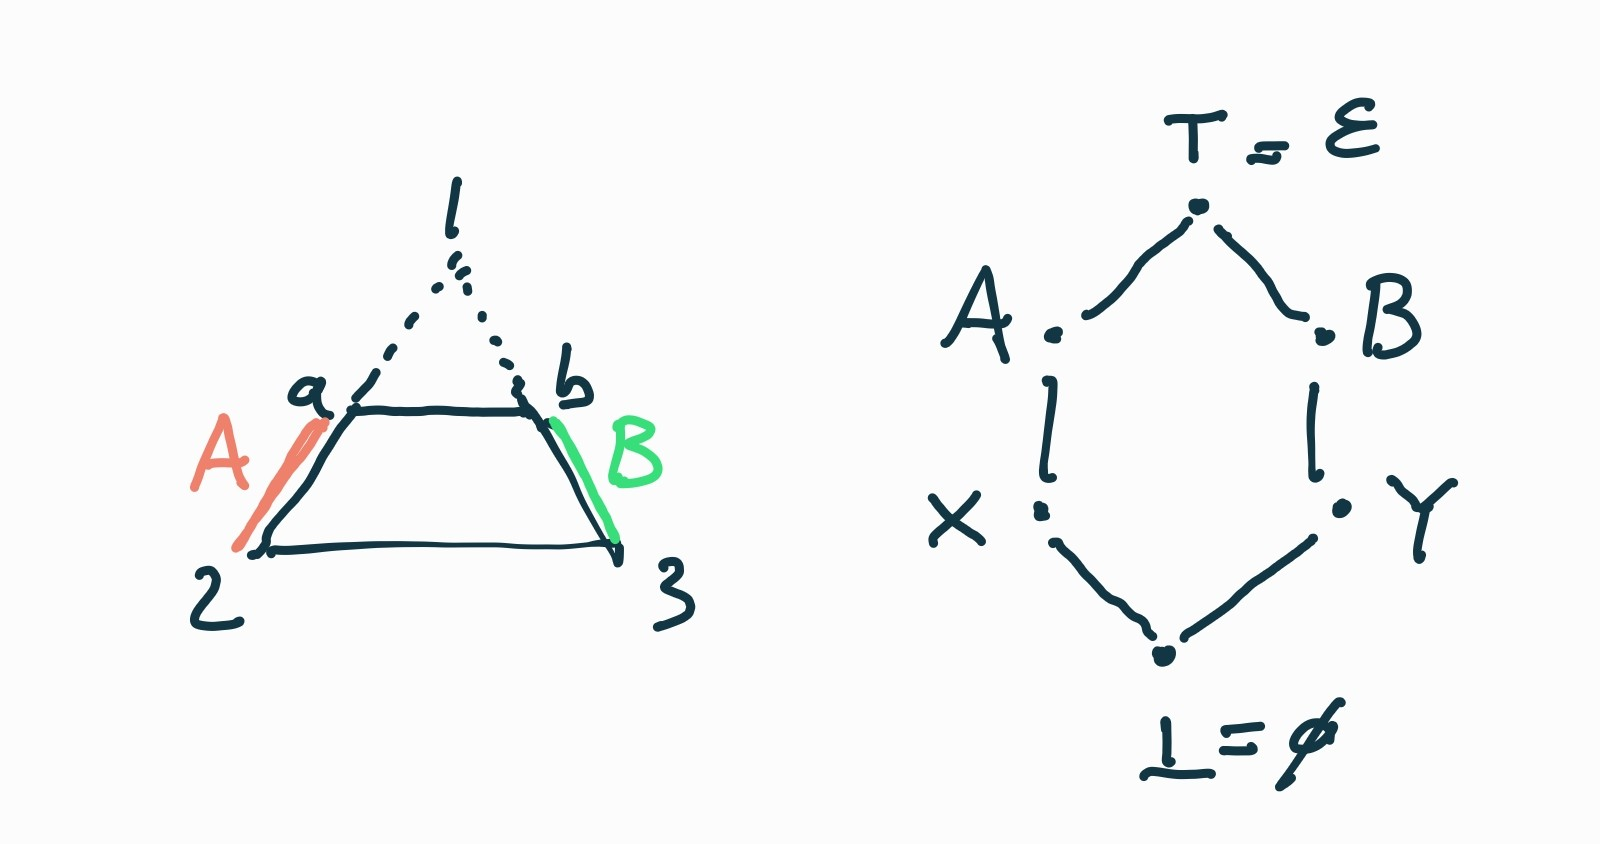
\includegraphics[width=0.7\textwidth]{tempimages/CutTriangleSubspaces.jpg}\label{pm_es_figCutTriangleOrthoSubspaces}\caption{On the left, the cut triangle. On the right, the diagram of the orthogonal subspaces.}
\end{figure}

The lack of orthonormality is due to the multiple complements that are one a subset of the other. This means that $X \vee (X^\perp \wedge A) = X \vee (B \wedge A) = X \vee \bot = X$ instead of $A$, if the lattice where orthonormal. This leads to the following:
\begin{conj}
	The lattice of $\separate$-subspaces is orthonormal if and only if the ensemble space is orthogonally decomposable (i.e. every decomposable ensemble is orthogonally decomposable).
\end{conj}
If this is true, the requirement of orthonormality is an additional requirement that can be understood physically.

Note, however, that the lattice of $\separate$-subspaces  of the cut triangle is orthonormal, though not commutative. This shows how the two lattices can be very different.

\begin{figure}[h]
	\centering
	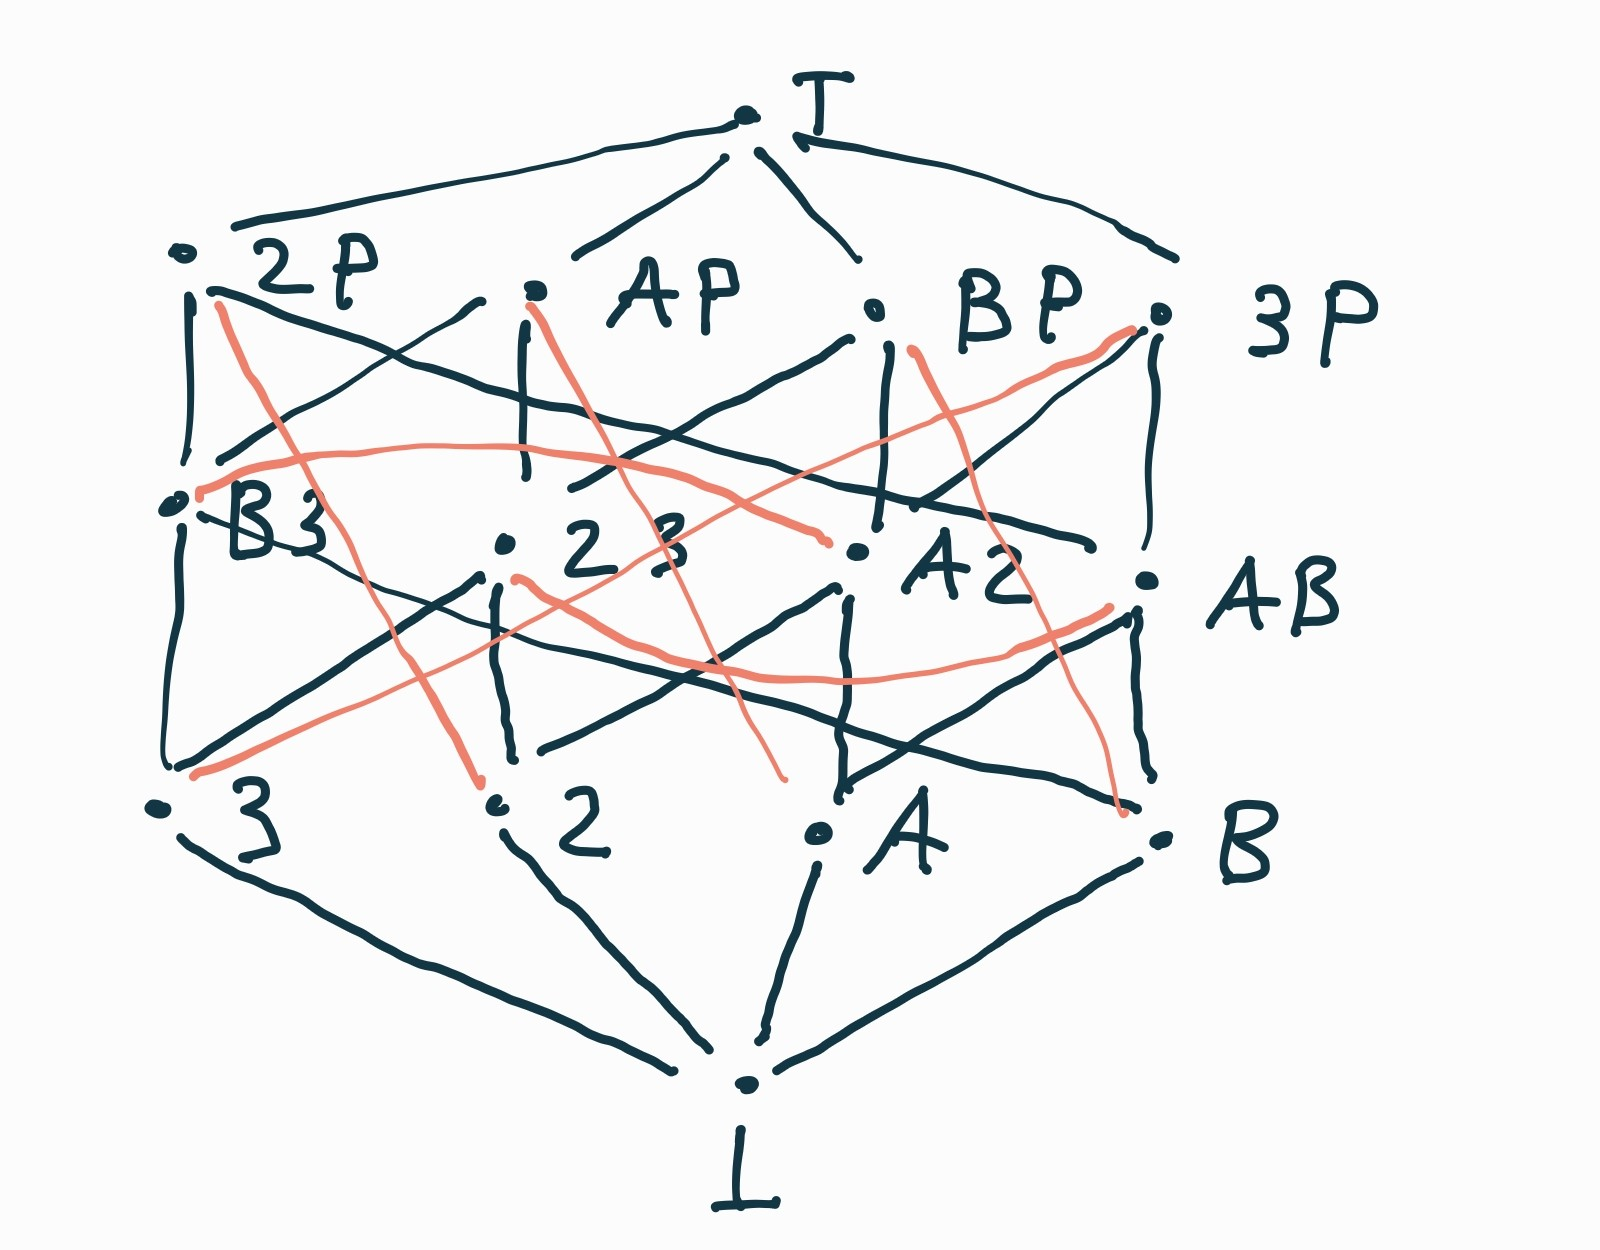
\includegraphics[width=0.7\textwidth]{tempimages/CutTriangleSubspaces2.jpg}
	\caption{In this diagram, the lower tier represents the singletons of the extreme points, the middle tier represents each side and the top tier represent the pairs of sides that are the $\separate$-complement of the extreme points. Note that the lattice is not a distributive (e.g. $A\vee (3 \wedge A2) = A \vee \bot = A \neq (A\vee 3) \wedge (A \vee A2) = BP \wedge A2 = A2$). In fact, $\{\bot, 3, A, A2, BP\}$ is an $N_5$ sub-lattice. }
\end{figure}



\section{Examples}

In this section we explore some examples that appear throughout the discussion to exemplify some corner cases, some wanted and some unwanted.

\begin{example}[Cut triangle]\label{pm_es_cutTriangle}
	The cut triangle is the subset of probability measures over three elements where the probability of the first is constrained to be no more than $\frac{1}{2}$.
\end{example}

This ensemble space is the standard two simplex, a triangle, where the top is cutoff. This is the space of probability distributions $[p_1, p_2, p_3]$ such that $p_1 \leq \frac{1}{2}$, where entropy is the Shannon entropy. The extreme point of the space are $\ens[2] = [0,1,0]$, $\ens[3] = [0,0,1]$, $\ens[a] = [\frac{1}{2},\frac{1}{2},0]$ and $\ens[b] = [\frac{1}{2},0,\frac{1}{2}]$. Every ensemble that is decomposable is also separately decomposable but not necessarily orthogonally decomposable. Most ensembles, all those in the interior, are also separately multidecomposable. For example, $\ens[c]$ can be expressed as a mixture of $\ens[a]$ and $\ens[3]$, and of $\ens[b]$ and $\ens[2]$.

\begin{example}[Real interval with right topology]
	Let $\Ens$ be the interval $[0,1] \subset \mathbb{R}$ with the topology generated by sets of the form $(r,1]$. Since the topology is not $T_1$, it cannot be an ensemble space, but the mixing operation is continuous.
\end{example}

TODO: show that the mixing operation is continuous.

\section{Lessons learned}

This section summarized previous attempt that turned out to be failures. These lead to critical insights and therefore are kept here for reference.

\subsection{Entropy and convex structure}

\begin{insight}
	The entropy is not uniquely determined by the convex structure.
\end{insight}

When defining the entropy given a space of probability distributions, there is typically an underlying assumption that all ``pure states'' are equivalent. That is, they have the same entropy. For example, in a discrete classical space, the entropy is typically $-\sum_i p_i \log p_i$ which assumes the entropy is zero for all extreme points. This assumption is not tenable in general.

\begin{example}[Mixed gas]
	Let's assume we have a mixture of two gasses at a fixed temperature and volume. The state is therefore defined by the variables $n_a$ and $n_b$. The entropy of each configuration is $\log 1 = 0$. If we have a uniform distribution over $[1,N_a]$ for $n_a$ and $[1,N_b]$ cases of $n_b$, the total number of cases is $N_a N_b$, and therefore the entropy of the joint state is $\log (N_a N_b)$. Now, suppose we cannot control the number of molecules for each gas, but only the total $n$. Each value of $n$ will not correspond the same variability of the elements of the ensemble. If we fix $n$ number of particles, in fact, there will be $n+1$ configuration possible, and therefore the entropy of each case should be $\log (n+1)$.
	
	If we have the space of probability distribution over a single variable that represents the total number of particles, then we would not be able to know whether these are all indistinguishable or divided into two distinct types. Therefore we would not know which is the correct physical entropy.
\end{example}

Note that in quantum mechanics there is a tacit assumption that all states have the same entropy. We could imagine, however, a theory where the pure states, the ones that we can ideally prepare and control, are not all at the same entropy. This would bake into the space state that not all evolutions are reversible. There is no reason to exclude this case, and it may turn out to be what we need for future theories.

\subsection{Continuity of affine combinations}

\begin{insight}
	Mixing cannot be a homeomorphism.
\end{insight}

To answer whether the embedding of the ensemble space in the topology of the vector space is continuous, we wanted to understand whether the inverse of the mixing is continuous. Turns out, it can't be in general because of the extreme points.

\begin{prop}
	Let $\Ens = [0,1]$ and suppose that mixing is a homeomorphism, meaning $+_{p \ens[a]}(\ens[b]) = p\ens[a] + \bar{p}\ens[b]$ is a homeomorphism onto its image. Then $\Ens$ would have to have the discrete topology, which is not possible, since the topology must be second countable.
\end{prop}

\begin{proof}
	Consider $+_{\frac{1}{2}0}([0,1])= [0,\frac{1}{2}]$. Since $[0,1] = \Ens$ is an open set, then $[0,\frac{1}{2}]$ is an open set as $+_{\frac{1}{2}0}([0,1])$ is a homeomorphism. Similarly, $+_{\frac{1}{2}1}([0,1])= [\frac{1}{2},1]$ is an open set. This means that $\{\frac{1}{2}\} = [0,\frac{1}{2}] \cap [\frac{1}{2},1]$ is an open set. This means that, for every $p \in [0,1]$, $+_{p0}(\{\frac{1}{2}\})= \{\{\frac{1}{2}(1-p)\}$ is an open set. Similarly, for every $p \in [0,1]$, $+_{p1}(\{\frac{1}{2})= \{\frac{1}{2}(1+p)\}$ is an open set. This means that every singleton is open, and the topology is discrete. The topology, then, cannot be second countable and $\Ens$ cannot be an ensemble space.
\end{proof}

Note that, in the above example, $+_{\ens[a]\ens[b]} : [0,1] \to \Ens$ would also fail to be a homeomorphism, though it is not clear how this is related to the failure of continuous embedding in a topological vector space (probably failure of scalar multiplication?).

The continuity of the mixing function means we can stretch open sets and still have open sets, but not, in general, shrink them. In retrospect, this makes sense as the bounds created by the boundaries of the convex set are of a different nature than the bounds of a finite precision measurement.

\subsection{Convergence of points without converge of fraction}

\begin{insight}
	In a limit, the fraction does not necessarily converge to one.
\end{insight}

Since the fraction tells us how much an ensemble is part of another, an intuitive conjecture would be that if $\ens[a]_i \to \ens[a]$ then $\size_{\ens[a]}(\ens[a]_i) \to 1$. That is, the fraction increases as we get closer to the limit. This does not work because one can make a limit over the extreme point.

\begin{example}[Pure state convergence in a quantum space]
	Let $\psi_i$ be a sequence of pure states and $\psi$ a pure state such that $\psi_i \to \psi$. For example, on Bloch sphere, it would be a sequence of points on the surface that converges to a point on the surface. Then, since they are all pure states, we have $\size_{\psi}(\psi_i) = 0$. This means $\psi_i \to \psi$ while $\size_{\psi}(\psi_i) \to 0 \neq 1$.
\end{example}

\subsection{Measures and topology}

\begin{insight}
	Boundaries of open sets can have non-zero measure.
\end{insight}

An earlier attempt of trying to find a compatibility condition between measures and topology was to impose that boundaries of open sets have measure zero. The idea was that we cannot associate measure to non-terminating conditions. Though the conceptual idea is sensible, the specific implementation does not work. We can find a counterexample on the real line. 

\begin{prop}
	Let $\mu$ be the Lebesgue measure on the real line $\mathbb{R}$. There exists an open set $U$ such that $\mu(U) \neq \mu(\overline{U})$.
\end{prop}

\begin{proof}
	Let $C$ be \href{https://en.wikipedia.org/wiki/Smith%E2%80%93Volterra%E2%80%93Cantor_set}{Smith–Volterra–Cantor}. This is a closed set with no interior for which $\mu(C) = \frac{1}{2}$. Let $U = (0,1) \setminus C$. We have that $U$ is an open set and with $\overline{U} = [0,1]$. We have $\mu(\overline{U}) = \mu([0,1]) = 1$ while $\mu(U) = \mu([0,1]) - \mu(C) = \frac{1}{2}$.
\end{proof}

\subsection{Subspaces from convex structure}\label{pm_es_failureConvexSubspace}

\begin{insight}
	The convex structure, by itself, cannot define subspaces.
\end{insight}

Initially, we tried recovering the notion of subspaces purely from the convex structure. We did make some progress in the finite dimensional case, but ultimately this does not work. We identified two problems.

The original definition was as follows.

\begin{defn}
	Let $\Ens$ be a convex space and $X \subseteq \Ens$ be a subset. We say that $X$ is a \textbf{subspace} of $\Ens$ if it contains all the convex combinations and all the components of its elements. That is, for every $\ens_1, \ens_2, \ens_3 \in \Ens$ and $\lambda \in (0,1)$ such that $p \ens_1 + \bar{p} \ens_2 = \ens_3$ we have:
	\begin{itemize}
		\item $\ens_1, \ens_2 \in X$ implies $\ens_3 \in X$
		\item $\ens_3 \in X$ implies $\ens_1, \ens_2 \in X$.
	\end{itemize}
	The \textbf{convex span} of $X$, noted $\cospan(X)$, is the smallest subspace containing $X$.
\end{defn}

\begin{remark}
	As defined, the convex span of two elements will include all their possible mixtures (i.e. the segment that connects them), all possible decompositions (i.e. all lines that pass through them) plus, recursively, all other mixtures and decompositions that can be reached from those. Physically, the idea is that if we act on some ensembles, then we are also acting not them but we are acting on all its components. Therefore, the proper definition of subspace does not include just the mixtures, but all possible components and all their possible mixtures.
\end{remark}

\begin{example}[Classical discrete spaces]
	Let $S$ be a set of $n$ possible discrete states and let $\Ens$ the space of probability distributions over the set $S$ (i.e. $\Ens$ is an $n$-simplex and $S$ are its extreme points). A subspace $X$ of $\Ens$ is a convex hull of a subset $U$ of $S$. That is, a subspace of $\Ens$ is the space of probability distributions over a subset of the cases. Geometrically, it is one of the sides (possibly recursively) of the simplex.
	
	To see this, first note that the convex hull $X$ of any subset $U$ of extreme points $S$ is a subspace. In fact, it will contain all convex combinations of $U$, and any element can only be decomposed in convex combinations of $U$. Second, note that only convex hulls of a subset of extreme points can be a subspace. In fact, any element of $\Ens$ can be expressed as a non-trivial convex combination of a set of extreme points $U$. Therefore, if an element is present in a subspace $X$, then $U \subset X$, which means all elements of the convex hull of $U$ are in $X$.
\end{example}

\begin{example}[Finite dimensional quantum spaces]
	Let $\mathcal{H}$ be an $n$-dimensional Hilbert space and let $\Ens$ be the space of density matrices (i.e. positive semi-definite self-adjoint operators with trace one). A subspace $X$ of $\Ens$ is the space of density matrices of a subspace $U$ of $\mathcal{H}$. That is, a subspace of $\Ens$ is the space of mixed states over a subspace of pure states.
	
	To see this, first note that the space of density matrices $X$ of a subspace $U$ of $\mathcal{H}$ is a subspace of $\Ens$. In fact, $X$ it will contain all convex combinations of its elements. Moreover, any element $x \in X$ can only be decomposed in a convex combination of pure states of $U$. Therefore any convex decomposition of $x$ has all its elements in $X$. Second, note that only the space of density matrices $X$ of a subspace $U$ of $\mathcal{H}$ is a subspace of $\Ens$. In fact, any element $x$ of $\Ens$ can be expressed as a non-trivial convex combination of orthogonal pure states, its eigenstates. These elements will span a subspace $U$ of $\mathcal{H}$. From those elements, we can construct an equal mixture which represents the maximally mixed states and, mathematically, is the identity operator $I/m$ divided by the number of elements $m \leq n$ of $U$. The equal mixture of any orthogonal basis of $U$ will also give the maximally mixed state. Therefore, given an element $x$, any subspace that contain $x$ will also contain a basis of $U$, the maximally mixed state $I/n$, all possible basis of $U$, which means all the pure states, and finally all convex combinations of the pure states, which means all possible density matrices, all possible mixed states.
\end{example}

The definition works in these cases, which is why it looked promising, but not in general.

\begin{insight}
	Rate of convergence cannot be changed by a convex combination.
\end{insight}

\begin{prop}
	Let $\Ens$ be the space of probability measures over $[0,1]$. Let $\ens[a]$ be the uniform distribution and let $\ens[b]$ be a distribution whose density goes to zero at the endpoints. Then $\ens[b]$ is a component of $\ens[a]$ but not vice-versa. Therefore the convex span of $\ens[a]$ is the whole $\Ens$ while the convex span of $\ens[b]$ is not the whole $\Ens$.
\end{prop}

\begin{proof}
	Consider the two probability densities $\rho_a$ and $\rho_b$ associated with the ensembles. The density $\rho_b$ has a supremum $\sup \rho_b$ that is greater than $1$, which means $p = \frac{1}{\sup \rho_b}$ is smaller than one. The function $\rho_c = \frac{1}{\bar{p}} \rho_a - \frac{p}{\bar{p}}\rho_b$ will be a non-negative function that integrates to one. The same procedure could be applied for any probability density, which means every probability measure over $[0,1]$ is a component of the uniform distribution. Therefore the convex span of $\ens[a]$ is the whole $\Ens$.
	
	Conversely, consider a possible convex combination $p \rho_a + \bar{p} \rho_c = \rho_b$. Since $\rho_b$ converges to zero at the endpoints, for each $p$ there will be a neighborhood of $0$ for which $p\rho_a$ is greater than $\rho_b$. Therefore $\rho_c$ cannot be a non-negative function. This means that $\ens[a]$ is not a component of $\ens[b]$ and the convex span of $\ens[b]$ is not the whole $\Ens$.
\end{proof}

This means that this notion of subspace does not simply return all the function with the same support, but the function with the same support and a particular class of convergence on the boundaries, and possibly at interior points.

One key problem is that it cannot be generalized to the classical continuous case, as the rate of convergence cannot be changed by finite convex combinations. Even if that problem is fixed, there would be nothing to determine the dimensionality of $U$, and we could create convex maps that ``stretch'' the space. This lead to the following:

\begin{insight}
	Dimension/count of states cannot be determined by the convex structure.
\end{insight}

Even if the previous problem is solved, the ``size'' of the subspace cannot be determined with a convex structure alone. In the finite dimensional case this works, but in the infinite dimensional case it does not. 

\begin{prop}
	Let $X=M_1([0,1])$ and $Y=M_1([0,2])$ be the spaces of probability measures on $[0,1]$ and $[0,2]$ respectively. The function $f : [0,1] \to [0,2]$ such that $f(x) = 2x$ is a diffeomorphism and induces a bijective continuous affine map between $M_1([0,1])$ and $M_1([0,2])$. However, the entropy is not conserved through the map.
\end{prop}

\begin{defn}
	In terms of the probability measures, the map simply acts on the transformed sets. That is, $\mu_Y(A) = \mu_X(f^{-1}(A))$. This, for example, maps the uniform distribution over $[0,1]$ to the uniform distribution over $[0,2]$. Therefore $A$ and $B$ are isomorphic as convex spaces. However, the entropy over a uniform distribution changes with the range, therefore the entropy is not conserved through the map.
\end{defn}

This means that the convex structure and the topology are not enough to determine the size of the space. This means that, without information about the entropy, we are not going to be able to tells that we spread ensembles over double the distance.


\subsection{Spectrum from subspaces}

\begin{insight}
	The lattice of subspaces is not enough to recover the points.
\end{insight}

Originally, we intended to recover the spectrum of an operator (i.e. the values possible values over which the distribution is defined) by taking the limit of subspaces. For example, for position a possible value $x$ would be the limit of the sequence of subspaces of distributions with support $[x-\epsilon, x+\epsilon]$. Formally, the construction was similar to the \href{https://en.wikipedia.org/wiki/Stone%27s_representation_theorem_for_Boolean_algebras}{Stone's representation theorem for Boolean algebras}, and the points were the ultrafilters. However, this does not work as the ultrafilters are ``too fine.'' When reconstructing a real line, for example, the limit approaching from below and the limit approaching from above would be two separate points.

The core of the problem is that the lattice of subspaces recover the Boolean algebra of the regular open sets. However, the lattice of the regular open sets is not enough to reconstruct the points of the space.

\begin{prop}[Regular open sets are not enough]\label{pm_es_regularOpenSetsNotEnough}
	Let $X$ and $Y$ be two topological spaces such that the respective lattices of regular open sets $R_X$ and $R_Y$ are isomorphic as Boolean algebras. It does not follow that $X$ and $Y$ are homeomorphic as topological spaces.
\end{prop}

\begin{proof}
	Let $X=S^1$ be a circle with the standard topology, $Y=\mathbb{R}$ be the real line with the standard topology and $Z=\mathbb{R}\setminus \{0\}$ be the real line without the origin. Note that the circle is the one point compactification of the real line, and therefore $Y=X\setminus \{\infty\}$. This forms a chain of embedding $Z \to Y \to X$.
	
	Suppose $U_X$ is a regular open set in $X$. Then $U_Y = U_X \setminus \{\infty\}$ is an open set in $Y$. We also have $\overline{U_Y} = \overline{U_X} \setminus \{\infty\}$ and $\interior(\overline{U_Y}) = \interior(\overline{U_X}) \setminus \{\infty\}$ where the closure and interior are taken in the respective spaces. Therefore $U_Y$ is a regular open set. Also, let $U_X$ and $V_X$ be two distinct open sets of $X$. Then, since every open set that contains $\{\infty\}$ also contains an open neighborhood of $\{\infty\}$, the corresponding $U_Y$ and $V_Y$ will also be two distinct open sets. Then $\iota(U_X) = U_X \setminus \{\infty\}$ is an injection between the regular open sets of $X$ and $Y$. Now let $U_Y$ be a regular open set on $U$. Let $U_X = \interior(\overline{U_Y \cup \{ \infty \}})$ where the  closure and interior are taken in $X$. Then $U_X$ is a regular open set of $X$ because it is the interior of a closure. Also note that $\interior(\overline{\iota(U_X) \cup \{ \infty \}}) = \interior(\overline{U_X \setminus \{\infty\} \cup \{ \infty \}}) = \interior(\overline{U_X}) = U_X$. Therefore the map $\iota$ is a bijection between the regular open sets of $X$ and $Y$.
	
	Note that regular open sets form a Boolean algebra where the complement is the exterior, the join is the interior of the closure of the union and the meet is the intersection. Note that if $U_X \subset V_X$, then $\iota(U_X) \subset \iota(V_X)$, therefore $\iota$ preserves the joins and the meets. Now let $V_X = \exterior(U_X)$ and consider $\iota(V_X)$. This will contain all the exterior points of $U_X$ minus $\{\infty\}$. But these are also the exterior points of $\iota(U_X)$. Therefore $\exterior(\iota(U_X)) = \iota(\exterior(U_X))$. The bijection is an isomorphism of Boolean algebras, and the corresponding algebras of regular open sets are isomorphic. The same reasoning applies when comparing $Y$ to $Z$.
	
	Now, note that $\{\infty\}$ is a closed set, but not a regular closed set. Therefore we are going to be able to construct a similar argument for the lattice of regular closed sets
\end{proof}

Since the construction below wants to recover the points of the space from what happens to be the algebras of regular open (or closed) sets, the above proposition implies that this is not possible. We would not be able to know, for example, whether the points form a circle or a real line. Even if we knew that they form a real line, and would know what half-lines we have, we would not know how to stitch them back together, as we could do it with $\{0\}$ or with $\{\infty\}$. We would need to know, at least, which intervals would correspond to a finite interval (e.g. a finite entropy), which requires more structure.

\iftrue

\titledbreak{Experimental section}


\section{Fraction capacity and probability}

Having seen how the strict concavity of the entropy leads to geometric structures, we are going to see how mixing is responsible for the measure theoretic structures. In the same way we derived a geometric structure on the ensembles, we are going to first define a measure theoretic structure on the ensembles as well. This measure, the fraction capacity, will tell us how much of an ensemble can be seen as a mixture of a set of others. It is not additive in general, but subadditive.

We are then going to find necessary and sufficient conditions for a subset of ensembles to form a classical probability context, so that each element can be understood as a classical probability measure over a set of cases, over the spectrum of the context. We will see that all classical ensemble spaces are classical probability contexts, while in quantum mechanics the set of mixed states that commutes with a complete set of commuting observables corresponds to a classical probability context.\footnote{In the future we will want to generalize the construction of the spectrum to the whole space.}

\subsection{Topological measures}

Before showing when and how the fraction capacity reduces to a standard probability measure, we need to find which requirements a measure must satisfy to describe a well-posed physical problem. The issue is that the set of all probability measures defined over a space is too broad. The problem is not yet fully understood, so we limit there are articulating some problems.

If we restrict ourselves to the real line, given the Lebesgue measure $\mu$, \href{https://en.wikipedia.org/wiki/Lebesgue%27s_decomposition_theorem}{Lebesgue's decomposition theorem} assures us that every measure $\nu$ can be divided into these three components: an \href{https://en.wikipedia.org/wiki/Absolute_continuity#Absolute_continuity_of_measures}{absolutely continuous} part $\nu_{ac}$ with respect to the Lebesgue measure (i.e. $\nu_{ac}(U)=0$ for all sets $U$ for which $\mu(U)=0$), a pure point part $\nu_{pp}$ (i.e. there is a set of countable points $\{x_i\}$ such that $\nu_{pp}(\{x_i\}^{\complement})=0$) and a singular continuous part $\nu_{sc}$ (i.e. $\mu(\{x\})=0$ for all $x$ and there is a set $U$ such that $\mu(U)=0$ and $\nu_{sc}(U^{\complement})=0$).

To make this more concrete, let us assume that we are working on phase space, $\mu$ is the Liouville measure, which in statistical mechanics quantifies the states in a region, and $p$ is a probability measure. If $p$ is absolutely continuous with respect to $\mu$, it means that if a region has no states, it will have zero probability. This is the requirement under which the \href{https://en.wikipedia.org/wiki/Radon%E2%80%93Nikodym_theorem}{Radon-Nikodym theorem} applies and a probability density $\frac{dp}{d\mu}$ exists. Without this requirement, for example, the entropy cannot even be defined. On physics grounds, this requirement makes a lot of sense. A pure point measure would correspond to the case where the probability is concentrated into a few isolated points. In physics, these are often represented with delta functions. There is an inherent unphysicality of these measures: if we really have a continuum, it would make no sense to say that we are are able to prepare an exact value with certainty. We are essentially saying that we are able to concentrate the whole distribution on a set that is not experimentally verifiable (i.e. it is a closed set with no interior) and contains no states (i.e. the Liouville measure is zero). Yet, there are some cases where the distribution is over real values, but only certain values are allowed. For example, the mass spectrum for particles or the energy spectrum for a bound quantum system can only take certain values. In this case, the Lebesgue measure is the one that is meaningless, because the region in between the allowed value contains no physically meaningful cases. A singular continuous measure may be something physically irrelevant, like the \href{https://en.wikipedia.org/wiki/Cantor_distribution}{Cantor distribution} which is defined only on a Cantor set, but it may also represent a constrained distribution. For example, a uniform distribution over the surface of a sphere, if defined over three dimensional space, would have support on a measure zero set, and have zero probability at every point. The issue, again, is that the imposition of the constraint has to be applied to the whole mathematical structure, not just the probability measure.

Physically, we see that the requirement of experimental verifiability poses constraints on the measure. Mathematically, experimental verifiability is captured by the topology. Therefore the question is: when can we say that a measure is compatible with a topology? That is, instead of having relationships between measures, which ignore the topology, we should have a direct relationship between each measure and the topology. If two measures are compatible with the topology, then they should be automatically well-behaved with respect to each other.

Let us step back and think more broadly. Recall that an open set corresponds to an experimentally verifiable statement. Imagine we prepared a distribution over some variable, and have a test that tells us whether the value of an instance is within a specific range $U$. Then the open set $U$ corresponds to the positive outcome of the test. The exterior $\exterior(U)$ corresponds to the negative outcomes of our test. The boundary $\partial U$ corresponds to those cases we are not able to adjudicate experimentally: they are not in $U$, but are too close to $U$ to discern from $U$. That is, there is no test that can tell us we have an element of $\partial U$, these cases are not experimentally verifiable. It is not clear exactly what is the right specification to make sure we do not associate a probability or a count of possible cases to sets that cannot be associated to termination.

\subsection{Flats and affine combinations}

Having seen the type of classical probability measure each ensemble should reduce to, we now need to identify the correct closure condition for a set of ensembles to form a space of probability measures. Roughly speaking, we want to be able to think of the set of ``all'' the probability distributions over a set of cases. We have to clarify what we mean by ``all.''

Requiring the set of probability measures to be closed under convex combinations is not enough. The cut triangle \ref{pm_es_cutTriangle}, for example, is a subset of a discrete classical ensemble space where not all ensembles can be understood as a unique convex combination of the extreme points, precisely because some cases are missing. This convex subset is leaving out some ensembles, making a classical space not look classical. On the other hand, if we take a Bloch ball, we can take three points on the surface. These would form a triangle, which could be understood as a discrete classical probability space. Here the convex closure is leaving out some ensembles, making a non-classical space look classical. Therefore we first have to understand what the correct closure is before we can determine whether it forms a set of classical probability measures or not.

As an early attempt, we considered extending the closure to both mixtures and components. That is, closure on the mixtures would require $\ens[a] = p \ens[b] + \bar{p} \ens[c]$ to be in the set if both $\ens[b]$ and $\ens[c]$ are present. Closure on the components would also require $\ens[b]$ and $\ens[c]$ to be in the set if $\ens[a]$ is present. This seems to take too much in. In quantum mechanics, for example, a single mixed state would bring in all the mixed states in the smallest subspace that contains it. The problem is that we would never be able to carve out the spaces of classical probability measures that are associated with each quantum measurement context.

The correct closure seems to be to include all affine combinations. That is, if $\ens[a] = p \ens[b] + \bar{p} \ens[c]$ and two of the ensembles are in the set, then the other one is in the set as well. This allows us to get all the ensembles in the same hyperplane. We call this a flat. In the triangle example, the only flats available are the single vertexes, each side and the whole triangle. For the Bloch ball, if we took two elements, we would get the whole segment that connects them and extends to the surface. But if we get three points, we get a circle, which is not a simplex. This affine closure, essentially, allows us to remove ``ensembles from each other'' as much as possible, so that we can get to their most distinct, most separate, form.

% Reviewed with Christine start

\begin{mathSection}
	\begin{defn}
		A \textbf{simplex} is a subset $U \subset \mathbb{R}^n$ that is the hull of finitely many affinely independent points. That is, $U = \hull(\{x_i\}_{i=0}^{n})$ such that $\{x_i - x_0\}_{i=1}^{n}$ are linearly independent.
	\end{defn}
	
	\begin{defn}
		A \textbf{flat} $A \subseteq \Ens$ is a closed convex subset that contains all lines between all elements. That is, for any $\ens[a], \ens[b] \in A$, $A$ also contains the line that contains $\ens[a]$ and $\ens[b]$. Given a set $U \subseteq \Ens$, the \textbf{flat closure} of $U$ is the smallest flat that contains $U$. A flat is \textbf{finite} if it can be generated by a finite number of elements. An $n$-flat is a flat that must be generated by a set with at least $n$ elements.
	\end{defn}
	
	\begin{figure}[H]
		\centering
		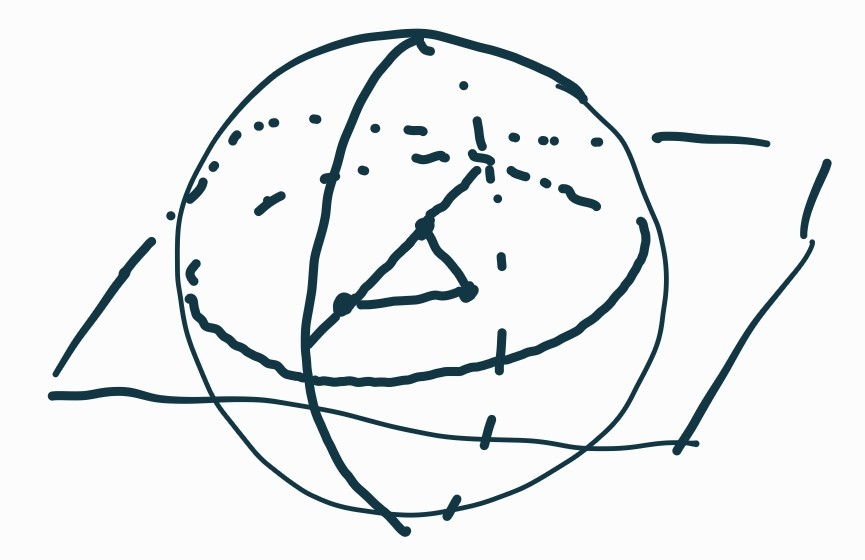
\includegraphics[width=0.4\textwidth]{tempimages/FlatVsConvex.jpg}
		\caption{Flat vs convex set. The ball is the ensemble space. The triangle represents a convex subset. The disc containing the triangle is the flat closure of the triangle. The plane is the affine closure of the triangle.}
	\end{figure}
	
	
	\begin{prop}
		A flat includes all possible affine combinations of elements of $\Ens$ that are contained in $\Ens$. The flat closure of $U \subseteq \Ens$ is the intersection of $\Ens$ with the affine closure of $U$ in the embedding vector space.
	\end{prop}
	
	\begin{proof}
		Let $A \subseteq \Ens$ be a flat and let $V$ be the real vector space that embeds $\Ens$. A line between two elements $\ens[a], \ens[b] \in A$ can be extended in $V$ and can be written as $\ens[a] + x \left(\ens[b] - \ens[a]\right)$ with $x \in \mathbb{R}$. Therefore any ensemble that can be written as an affine combination of two ensembles in $A$ is an element of the flat. Recursively, this means that any ensemble that can be written as an affine combination of finitely many ensembles in $A$ is also in the flat. Moreover, since the flat is a closed set, it will also include all its limits. Therefore every affine combination of $A$ that is also an element of $\Ens$ is in $A$, which means $A$ is the intersection of an affine subspace of the embedding vector space and the ensemble space.
		
		Now let $U \subseteq \Ens$ be a set of ensembles. The affine closure of $U$ will be an affine subspace of the embedding vector space. The flat closure will be the intersection of the affine closure with $\Ens$. Since the affine closure is the smallest closed affine subspace that contains $U$, its intersection with $\Ens$ will be the smallest flat that contains $U$, which is the flat closure of $U$.
	\end{proof}
	
	\begin{conj}
		An $n$-flat is a simplex if and only if its $3$-flats are simplexes (i.e. triangles).
	\end{conj}
	
	\begin{remark}
		In classical discrete ensemble spaces, any flat is a simplex. In classical continuous ensemble spaces, infinite dimensional flats will depend on what limits are allowed. In a quantum ensemble space, if we take three ensembles inside a Bloch ball, the corresponding flat will be a circle. If we take three orthogonal pure states, however, the corresponding flat will be a simplex.
	\end{remark}
\end{mathSection}

\subsection{Classical probability contexts}

Now that we have identified the correct closure, we need to find the right characterization of a flat to identify a classical probability context: a set of ensembles that can be characterized by a family of classical probability measures. For finite discrete spaces, we want to recover the notion of a simplex. In a simplex, every element has a single decomposition in terms of extreme points. This characterization does not work in infinite dimensions as there are no extreme points. As we saw before, the pure point probability measures are not, in general, continuous with respect to the topology. The trick, again, is being able to express this lack of multiple decompositions for finite mixtures.

%A classical probability context will be a set of ensembles that we will map to a space of measures. From the ensembles we will need to define the points over which the probability are defined, the spectrum of the context (in analogy to the spectrum of a linear operator). The general idea is that these will be limits of ensembles that become more and more concentrated, which will be characterized using tools from order theory and topology. Once the spectrum is defined, we will use the fraction capacity to define the probability measure over the topology of the spectrum.

%Technical details aside, we want definitions that capture the intuition of spaces of classical probability distributions in a way that works well for infinite dimensional spaces, is compatible with both discrete and continuous classical ensemble spaces but also with measurement contexts in quantum ensemble spaces. It is instructive to go through some of the different attempts to understand why we settled on these definitions, so that one can understand why they work.

\begin{mathSection}
	\begin{defn}
		An ensemble is \textbf{decomposable} if it can be expressed as a mixture of two distinct ensembles. An ensemble is \textbf{separately/orthogonally decomposable} if it can be expressed as a mixture of two separate/orthogonal ensembles. An ensemble is \textbf{separately multidecomposable} if it can be expressed as two decompositions where a component of one is separate from both components of the other. That is, $\ens = p \ens[a]_1 + \bar{p} \ens[a]_2 = \lambda \ens[b]_1 +\bar{\lambda} \ens[b]_2$ and either $\ens[a]_1 \separate \ens[b]_j$ or $\ens[a]_2 \separate \ens[b]_j$.
	\end{defn}
	
	\begin{figure}[H]
		\centering
		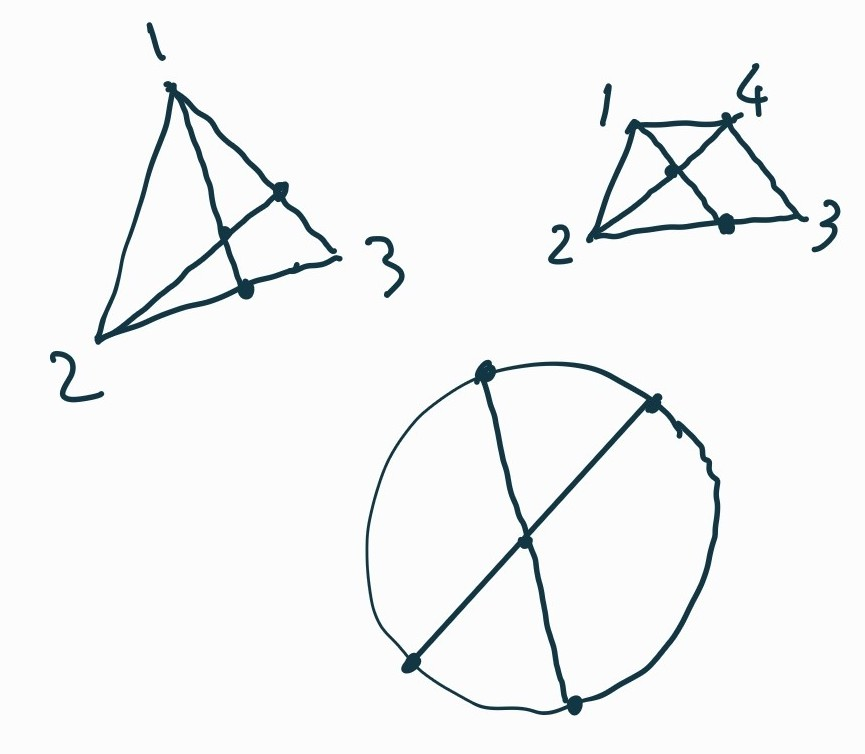
\includegraphics[width=0.4\textwidth]{tempimages/MultipleDecomposition.jpg}
	\end{figure}
	
	\begin{remark}
		Take a classical discrete space for three points which is a triangle (simplex). The only three elements that are not decomposable are the extreme points. Mixtures of two points are decomposable and are also separately decomposable in only one way. Mixtures of three points are also separately decomposable, but in multiple ways: as a mixture of $\ens_1$ and a mixture of $\ens_2$ and $\ens_3$, or as a mixture of $\ens_2$ and a mixture of $\ens_1$ and $\ens_3$. Note, however, that they are not separately multidecomposable as the different components are not separate.
		
		Take a Bloch ball for quantum mechanics. All the elements of the surface are not decomposable and they are all pairwise separate. The middle point can be seen as the equal mixture of any pair of opposite points. Therefore the middle point, as well as any other point not on the surface, is not only separately decomposable but also multidecomposable.
		
		To see why we require only one component to be separate from the other two, consider the cut triangle. Here we can have multiple decompositions where not all elements are separate.
	\end{remark}
	
	\begin{figure}[H]
		\centering
		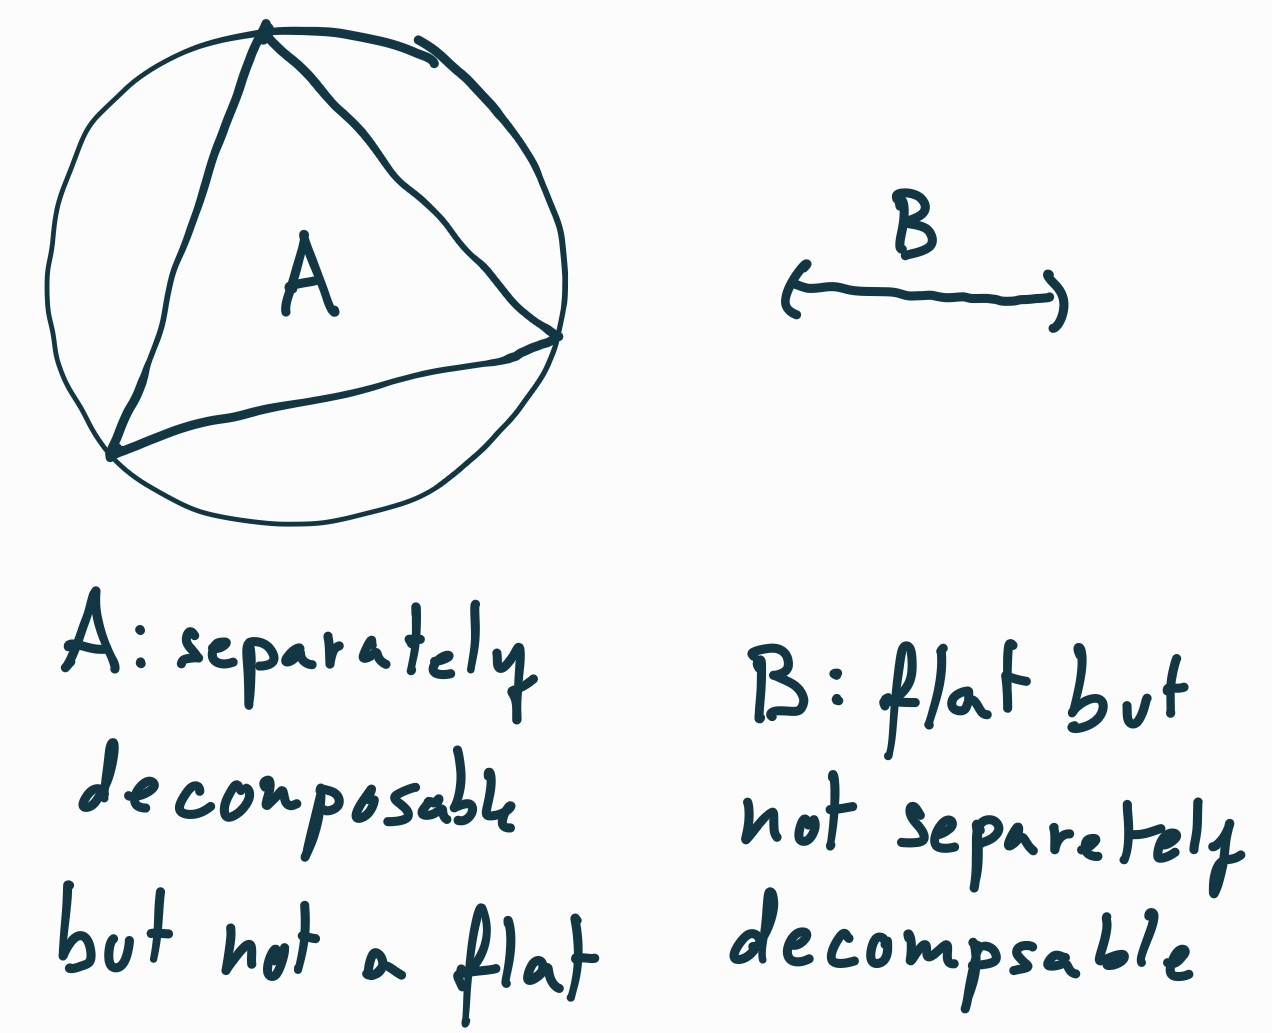
\includegraphics[width=0.4\textwidth]{tempimages/SeparableButNotFlat.jpg}
	\end{figure}
	
	\begin{remark}
		A convex set that is separately decomposable is not necessarily a flat (i.e. triangle within a sphere). A flat is not necessarily separately decomposable (i.e. open segment as a whole is a flat, but is not separately decomposable).
	\end{remark}
\end{mathSection}

\begin{mathSection}
	\begin{defn}
		Let $\Ens$ be an ensemble space. A \textbf{classical probability context} is a flat $C \subseteq \Ens$ where each decomposable element in $C$ is separately decomposable in $C$ but not separately multidecomposable in $C$.
	\end{defn}
\end{mathSection}

\begin{mathSection}
	\begin{prop}
		A flat $C \subseteq \Ens$ is a classical probability context if and only if every decomposable element is separately decomposable and mixtures preserve separateness in $C$. That is, if $\ens \separate \ens[a]$ and $\ens \separate \ens[b]$, then $\ens \separate p\ens[a] + \bar{p} \ens[b]$ in $C$ for all $\ens, \ens[a], \ens[b] \in C$ and $p \in [0,1]$.
	\end{prop}
	
	\begin{proof}
		Suppose mixtures do not preserve separateness. Then we can find $\ens,\ens[a],\ens[b], \ens[c] \in \Ens$ such that $\ens \separate \ens[a]$, $\ens \separate \ens[b]$ and $\ens \nseparate \ens[c] = p \ens[a] + \bar{p} \ens[b]$ for some $p \in (0,1)$. Since $\ens \nseparate \ens[c]$, we can find $\ens[d], \ens[f], \ens[g]$ such that $\ens[c] = \lambda \ens[d] + \bar{\lambda} \ens[f]$ and $\ens = \mu \ens[d] + \bar{\mu} \ens[g]$.  Since separateness extends to all mixtures (\ref{pm_es_separateExtendsMixtures}) and $\ens[a] \separate \ens[e]$, $\ens[a] \separate \ens[d]$ and, similarly, $\ens[b] \separate \ens[d]$, which means that $\ens[c]$ is separately multidecomposable.
		
		Now suppose mixture do preserve separateness, and let $\ens = p \ens[a]_1 + \bar{p} \ens[a]_2 = \lambda \ens[b]_1 +\bar{\lambda} \ens[b]_2$. Since $\ens[a]_1$ is a component of $\ens$, then $\ens \nseparate \ens[a]_1$. Since $\ens$ is a mixture of $\ens[b]_1$ and $\ens[b]_2$ and mixtures preserve separateness, then either $\ens[a]_1 \nseparate \ens[b]_1$ or $\ens[a]_1 \nseparate \ens[b]_2$. Similarly, $\ens[a]_2 \nseparate \ens[b]_1$ or $\ens[a]_2 \nseparate \ens[b]_2$. Therefore $\ens$ is not separately multidecomposable.
	\end{proof}
	
	\begin{conj}
		A convex subset $U \subseteq \Ens$ is a classical probability context if and only if all finite flats are simplexes.
	\end{conj}
	
	\begin{prop}
		Let $C \subseteq \Ens$ be a classical probability context. Let $U \subseteq C$ be a set of ensembles. Then $A=U^\separate=\{ \ens[a] \in C \, | \, \forall \ens \in U, \ens[a] \separate \ens \}$ and $B=(U^\separate)^\separate=\{ \ens[b] \in C \, | \, \forall \ens[a] \in A, \ens[b] \separate \ens[a] \}$ are two probability contexts such that $C = \hull(A \cup B)$.
	\end{prop}
	
	\begin{proof}
		First we show that $C$ contains only three types of ensembles: those that are limits of convex mixtures of $A$, those that are limits of convex mixtures of $B$ and those that are limits of convex mixtures of both $A$ and $B$. Any ensemble in $C$ is one of these three types. For $\ens[c] \in C$ to not be a mixture of $A$ or $B$, then $\ens[c]$ cannot be in either $A$ or $B$. This means that it must be separate from both $A$ and $B$. But $B$ contains all the elements that are separate from $A$, which is a contradiction. Since separate multidecomposition is forbidden, an ensemble $\ens$ cannot be written both as a convex combination of $A$ and as a convex combination with an element of $B$. This would yield two decompositions in which one component, the one chosen from $B$, is separate from all the components of the other. This means that an element of $C$ is either a mixture of $A$, a mixture of $B$ or a mixture of both $A$ and $B$.
		
		Now we show that both $A$ and $B$ are convex sets. Since a mixture of $A$ can only be expressed as a mixture of components of $A$, it is separate from all elements of $B$. Therefore $A$ contains all its mixtures. With the same logic, $B$ will contain all its mixtures. The argument works for infinite convex combinations as well. If $\ens = \sum_{i=1}^{\infty} p_i \ens[a]_i$ with $p_i \in [0,1]$ and $\sum_{i=1}^{\infty} p_i = 1$, it can be understood as the limit of the series $\frac{p_1}{P_n} \ens[a]_1 + \frac{\bar{p}_1}{P_n} \sum_{i=2}^{n} p_i \ens[a]_i$ where $P_n = \sum_{i=1}^{n} p_i$. Therefore
		\begin{equation}
			\begin{aligned}
				\ens &= \sum_{i=1}^{\infty} p_i \ens[a]_i = \lim\limits_{n \to \infty}  \sum_{i=1}^{n} \frac{p_i}{P_n} \ens[a]_i = \lim\limits_{n \to \infty} \frac{p_1}{P_n} \ens[a]_1 + \lim\limits_{n \to \infty}\frac{\bar{p}_1}{P_n} \sum_{i=2}^{n} \frac{p_i}{\bar{p}_1} \ens[a]_i = p_1 \ens[a]_1 + \bar{p}_1 \sum_{i=2}^{\infty} \frac{p_i}{\bar{p}_1} \ens[a]_i \\
				&= p_1 \ens[a]_1 + \bar{p}_1 \hat{\ens[a]}_1
			\end{aligned}
		\end{equation}
		where $\hat{\ens[a]}_1 = \sum_{i=2}^{\infty} \frac{p_i}{\bar{p}_1} \ens[a]_i$. Since $\ens$ and $\ens[a]_1$ are elements of the ensemble space, the series converges to $\hat{\ens[a]}_1$, which is in the hull of $A$. It will also be an element of $A$ because multidecompositions are forbidden.
		
		To see that $C$ is the hull of $A$ and $B$, note that all the elements in $C$ that are not already in $A$ or $B$ are the mixtures of $A$ and $B$. These are exactly added when taking the hull of $A \cup B$.
		
		Now we show that $A$ and $B$ are classical probability contexts. First we have to show that they are flats. Let $L$ be the line that connects two elements $\ens[a]_1, \ens[a]_2 \in A$. Take $\ens[a]_3 \in L$. If it is a mixture of $\ens[a]_1$ and $\ens[a]_2$ then it is an element of $A$. If $\ens[a]_1$ is a mixture of $\ens[a]_2$ and $\ens[a]_3$, since $\ens[a]_1$ cannot have a common component with $B$, and $\ens[a]_3$ is a component of $\ens[a]_1$, $\ens[a]_3$ cannot have components in $B$ as well. Therefore $\ens[a]_3$ must be a mixture of elements of $A$. Similarly if $\ens[a]_2$ is a mixture of $\ens[a]_1$ and $\ens[a]_3$. Therefore $A$ is a flat. Similarly, $B$ is a flat.
		
		Now we show that $A$, and by symmetry $B$, is a classical probability context. We have seen that $A$ is a flat. If an element of $A$ is decomposable in $A$ it is also decomposable in $C$ and is therefore separately decomposable in $C$. Because multidecomposability in $C$ is not allowed, it must be separately decomposable into elements of $A$. Lastly, if multidecomposability were allowed in $A$, it would also be allowed in $C$. Therefore it is not allowed in $A$. This means that $A$ is a classical probability context.
	\end{proof}
	
	\begin{figure}[H]
		\centering
		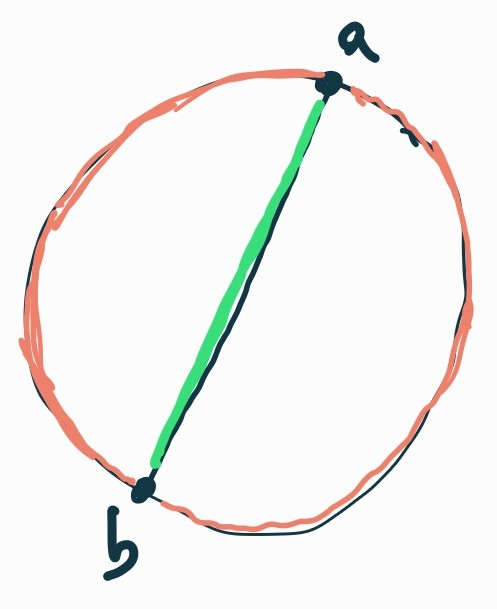
\includegraphics[width=0.25\textwidth]{tempimages/CounterexampleProbabilityContexts.jpg}
		\caption{TODO: make the final picture not go through the center, change the label for the points to $\ens_1$ and $\ens_2$}
	\end{figure}
	
	\begin{remark}
		Note that if multiple separate decompositions are not ruled out, the sub-contexts will not include all convex combinations. Take a disk as a convex space. Suppose $U$ is made of two points $\ens_1$ and $\ens_2$. All other points on the surface are separate from both and therefore belong to $A$. Now consider the convex combinations of $\ens_1$ and $\ens_2$. These are not separate from $U$ but they are also not separate from all the other elements on the surface. Therefore they are neither in $A$ nor $B$. Moreover, any other point in the interior can be seen as a convex combination of $\ens_1$ and another element of the surface that is not $\ens_2$. Therefore no point in the interior is in either $A$ or $B$. Thus $A$ and $B$ are not necessarily convex sets if $C$ is not a classical probability context.
	\end{remark}
	
	\begin{figure}[H]
		\centering
		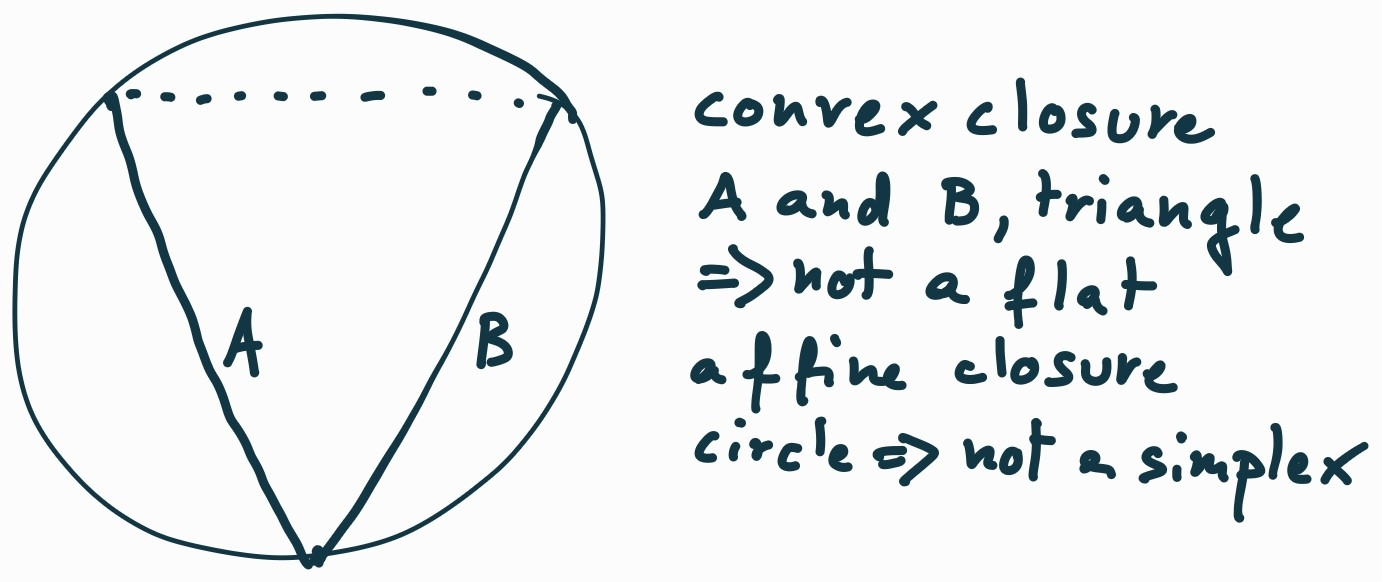
\includegraphics[width=0.75\textwidth]{tempimages/ContextClosureNotContext.jpg}
	\end{figure}
	
	\begin{remark}
		While a classical probability context can be decomposed into classical probability contexts whose closure is the original context, the converse is not true. That is, given two classical probability contexts, their convex or flat closure is not in general a classical probability context. Take a disk (the ensemble space) and two lines connecting three points (the two probability contexts). The convex closure is the triangle, which is not a flat as it misses some affine combinations. The flat closure is the disk, which is not a probability context.
	\end{remark}
	
	\begin{conj}
		Let $A, B \subseteq \Ens$ be two classical probability contexts. Then their flat closure and convex closure coincide if and only if these closures are a classical probability context.
	\end{conj}
	
	\begin{conj}
		The defining property of a classical probability context is exactly that property that allows $A$ and $B$ so constructed to be convex sets whose closure is $C$.
	\end{conj}
\end{mathSection}

\begin{prop}
	Let $C \subseteq \Ens$ be a classical probability context. The lattice of $\separate$-subspaces $\mathfrak{L}$ is distributive and is therefore a Boolean algebra.
\end{prop}

\begin{proof}
	Let $X,Y,Z \in \mathfrak{L}$ be three $\separate$-subspaces. Let $\ens \in X \wedge (Y \vee Z)$, then $\ens \in X$ and $\ens \in Y \vee Z$. This also means that all components of $\ens$ are in both $X$ and $Y \vee Z$ since the components of $\ens$ are not separate from $\ens$ and, given the absence of multi-decomposability, are separate from all elements that are separate from $\ens$. Since $Y \vee Z = \hull(Y \cup Z)$, we can decompose $\ens$ into components of $Y$ and $Z$. But these must be in $X$, and therefore $\ens \in \hull((X \wedge Y) \cup (X \wedge Z) ) = (X \wedge Y) \vee (X \wedge Z) )$. Therefore $X \wedge (Y \vee Z) \subseteq (X \wedge Y) \vee (X \wedge Z)$. Now let $\ens \in (X \wedge Y) \vee (X \wedge Z)$, then $\ens \in \hull((X \wedge Y) \cup (X \wedge Z) )$. Therefore $\ens$ is the mixture of ensembles that are in $X$, which means that $\ens \in X$. Since $\ens$ is the mixture of elements that are also in $Y$ and $Z$, $\ens \in \hull(Y \cup Z) = Y \vee Z$. This means $\ens \in X \wedge (Y \vee Z)$. Therefore $(X \wedge Y) \vee (X \wedge Z) \subseteq X \wedge (Y \vee Z)$. Which means $X \wedge (Y \vee Z) = (X \wedge Y) \vee (X \wedge Z)$.
	
	Now let $\ens \in X \vee (Y \wedge Z)$, then $\ens \in \hull(X \cup (Y \wedge Z) )$. That is, $\ens$ is a mixture of elements of $X$ and of elements that are in both $Y$ and $Z$. Which means $\ens \in \hull(X \cup Y)$ and $\ens \in \hull(X \cup Z)$. Therefore $\ens \in \hull(X \cup Y) \cap \hull(X \cup Z) = (X \vee Y) \wedge (X \vee Z)$, which means $X \vee (Y \wedge Z) \subseteq (X \vee Z) \vee (Y \wedge Z)$. Conversely, let $\ens \in (X \vee Y) \wedge (X \vee Z) = \hull(X \cup Y) \cap \hull(X \cup Z)$. Then $\ens$ can be expressed as a mixture of elements of $X$ and $Y$ and also of elements of $X$ and $Z$. Now consider the elements of $Y$ in the first decomposition. Since multiple decomposition is not allowed, they cannot be separate from both $X$ and $Z$, end therefore must be in their hull. Similarly, the elements of $Z$ in the second decomposition must be in the hull of $X$ and $Y$. Therefore $\ens \in \hull(X \cup (Y \wedge Z) ) = X \vee (Y \wedge Z)$. Therefore $(X \vee Y) \wedge (X \vee Z) \subseteq X \vee (Y \wedge Z)$. Which means $X \vee (Y \wedge Z) = (X \vee Z) \vee (Y \wedge Z)$.
	
	The lattice $\mathfrak{L}$ is therefore a distributive orthocomplemented lattice, which means it is a Boolean algebra.
\end{proof}

\begin{mathSection}
	\begin{prop}
		Let $C \subseteq \Ens$ be a classical probability context. Let $\mathfrak{L}$ be the lattice of $\separate$-subspaces. Then the fraction capacity is an additive set function on the lattice. That is, for all $\ens \in C$ and $A, B \in \mathfrak{L}$ such that $A \cap B = \emptyset$,  $\fcap_{\ens}(A \vee B) = \fcap_{\ens}(A) + \fcap_{\ens}(B)$.
	\end{prop}
	
	\begin{proof}
		Let $A, B\in \mathfrak{L}$ such that $A \cap B = \emptyset$. Then $A$ is separate from $B$. Therefore $A \vee B$ is a classical probability context that is the convex closure of two separate probability contexts. Therefore, as we saw in a previous proof, $A \vee B$ consists of convex combinations of $A$, which are all in $A$, of convex combinations of $B$, which are all in $B$, and of convex combinations of both, which are in neither $A$ nor $B$.
		
		We want to show that $\fcap_{\ens}(A \vee B) = \fcap_{\ens}(A) + \fcap_{\ens}(B)$ if $\ens \in A \vee B$. Let $\ens \in A \vee B$ be an ensemble that is the mixture of elements of $A$. Then $\ens \in A$ and it has no components in $B$. Therefore $\fcap_{\ens}(A \vee B) = 1$ and $\fcap_{\ens}(A) = 1$ while $\fcap_{\ens}(B) = 0$. This means $\fcap_{\ens}(A \vee B) = 1 = 1 + 0 = \fcap_{\ens}(A) + \fcap_{\ens}(B)$. If $\ens$ is a mixture of elements of $B$, we get the same conclusion. The last case is when $\ens$ is a mixture of elements of $A$ and $B$. That is, $\ens = \sum_i p_i \ens[a]_i + \sum_j \lambda_j \ens[b]_j$ with $\ens[a]_i \in A$, $\ens[b]_j \in B$, $p_i, \lambda_j \in [0,1]$ and $\sum_i p_i + \sum_j \lambda_j = 1$. By definition of fraction capacity, $\sum_i p_i \leq \fcap_{\ens}(A)$. Suppose $\sum_i p_i < \fcap_{\ens}(A)$. Then there is $\hat{\ens[a]} \in A$ such that $\ens = \sum_i p_i \ens[a]_i + p \hat{\ens[a]} + \lambda \ens[c]$ for some $p,\lambda \in [0,1]$ and $\ens[c] \in A \vee B$. But then $\ens$ would be separately multidecomposable, which is a contradiction since it is an element of a classical probability context. Therefore $\sum_i p_i = \fcap_{\ens}(A)$. Similarly, we find that $\sum_j \lambda_j = \fcap_{\ens}(B)$. Since $\sum_i p_i + \sum_j \lambda_j = 1$, $\fcap_{\ens}(A) + \fcap_{\ens}(B) = 1 = \fcap_{\ens}(A \vee B)$ for all $\ens \in A \vee B$.
		
		Now let $\ens \in C$. We have $(A \vee B)^\separate \in \mathfrak{L}$ and $(A \vee B) \cap (A \vee B)^\separate = \emptyset$. Therefore $\fcap_{\ens}(C) = \fcap_{\ens}(A \vee B)+ \fcap_{\ens}((A \vee B)^\separate)$. Note that $\ens$, in general, is a convex combination of elements of $A\vee B$ and $(A \vee B)^\separate$. Components in $A \vee B$ are convex combinations of elements of $A$ and $B$, which also disjoint. Therefore $\ens$ is a convex combination of elements of $A$, $B$ and $(A \vee B)^\separate$, which are pairwise disjoint. As before, since multidecomposability is forbidden in a classical probability context, the sum of the coefficients for each part will have to match the fraction capacity of its subcontext. Therefore $\fcap_{\ens}(A) +  \fcap_{\ens}(B) + \fcap_{\ens}((A \vee B)^\separate) = \fcap_{\ens}(C) = \fcap_{\ens}(A \vee B) + \fcap_{\ens}((A \vee B)^\separate)$. Thus $\fcap_{\ens}(A \vee B) = \fcap_{\ens}(A) +  \fcap_{\ens}(B)$ for all $\ens \in C$.
	\end{proof}
\end{mathSection}

\subsection{Spectrum of a classical probability context}

WARNING: the following may imply that the construction below doesn't work. Since we can show that different topological spaces correspond to the same Boolean algebra of regular open sets (or regular closed sets), then knowing the lattice of regular open (or closed) sets is not enough to recover the points and the topology.

\begin{prop}[Regular open sets are not enough]\label{pm_es_regularOpenSetsNotEnough}
	Let $X$ and $Y$ be two topological spaces such that the respective lattices of regular open sets $R_X$ and $R_Y$ are isomorphic as Boolean algebras. It does not follow that $X$ and $Y$ are homeomorphic as topological spaces.
\end{prop}

\begin{proof}
	Let $X=S^1$ be a circle with the standard topology, $Y=\mathbb{R}$ be the real line with the standard topology and $Z=\mathbb{R}\setminus \{0\}$ be the real line without the origin. Note that the circle is the one point compactification of the real line, and therefore $Y=X\setminus \{\infty\}$. This forms a chain of embedding $Z \to Y \to X$.
	
	Suppose $U_X$ is a regular open set in $X$. Then $U_Y = U_X \setminus \{\infty\}$ is an open set in $Y$. We also have $\overline{U_Y} = \overline{U_X} \setminus \{\infty\}$ and $\interior(\overline{U_Y}) = \interior(\overline{U_X}) \setminus \{\infty\}$ where the closure and interior are taken in the respective spaces. Therefore $U_Y$ is a regular open set. Also, let $U_X$ and $V_X$ be two distinct open sets of $X$. Then, since every open set that contains $\{\infty\}$ also contains an open neighborhood of $\{\infty\}$, the corresponding $U_Y$ and $V_Y$ will also be two distinct open sets. Then $\iota(U_X) = U_X \setminus \{\infty\}$ is an injection between the regular open sets of $X$ and $Y$. Now let $U_Y$ be a regular open set on $U$. Let $U_X = \interior(\overline{U_Y \cup \{ \infty \}})$ where the  closure and interior are taken in $X$. Then $U_X$ is a regular open set of $X$ because it is the interior of a closure. Also note that $\interior(\overline{\iota(U_X) \cup \{ \infty \}}) = \interior(\overline{U_X \setminus \{\infty\} \cup \{ \infty \}}) = \interior(\overline{U_X}) = U_X$. Therefore the map $\iota$ is a bijection between the regular open sets of $X$ and $Y$.
	
	Note that regular open sets form a Boolean algebra where the complement is the exterior, the join is the interior of the closure of the union and the meet is the intersection. Note that if $U_X \subset V_X$, then $\iota(U_X) \subset \iota(V_X)$, therefore $\iota$ preserves the joins and the meets. Now let $V_X = \exterior(U_X)$ and consider $\iota(V_X)$. This will contain all the exterior points of $U_X$ minus $\{\infty\}$. But these are also the exterior points of $\iota(U_X)$. Therefore $\exterior(\iota(U_X)) = \iota(\exterior(U_X))$. The bijection is an isomorphism of Boolean algebras, and the corresponding algebras of regular open sets are isomorphic. The same reasoning applies when comparing $Y$ to $Z$.
	
	Now, note that $\{\infty\}$ is a closed set, but not a regular closed set. Therefore we are going to be able to construct a similar argument for the lattice of regular closed sets
\end{proof}

\begin{remark}
	Since the construction below wants to recover the points of the space from what happens to be the algebras of regular open (or closed) sets, the above proposition seems to imply that this is not possible. We would not be able to know, for example, whether the points form a circle or a real line. Even if we knew that they form a real line, and would know what half-lines we have, we would not know how to stitch them back together, as we could do it with $\{0\}$ or with $\{\infty\}$. We would need to know, at least, which intervals would correspond to a finite interval (e.g. a finite entropy), which requires more structure.
\end{remark}

To recover classical probability distributions, we need to recover the possible cases (i.e. the sample space) and the events (i.e. the $\sigma$-algebra) over which the probability distributions are defined. These are not necessarily states. For example, in the countinuous classical case, the sample space corresponds to the sets of possible values of position and momentum (i.e. the symplectic manifold over which the values are defined). In quantum mechanics, the sample space is the range of possible values defined by an observable (i.e. the spectrum of the operator). The goal here is to identify a single physically meaningful construction that will be able to work for all these cases.

Intuitively, we are taking ensembles and decomposing them into mixtures of ensembles with narrower and narrower spread. The points over which the classical distributions are defined are limits where the spread goes to zero. Note, however, that the limit of sequences with narrower and narrower spread will not, in general, be itself an ensemble. For example, we can imagine a sequence of uniform distributions over $[-\frac{1}{i}, \frac{1}{i}]$. As $i$ increases, the spread will converge to the single value $0$, though the sequence of ensembles will not converge to an ensemble. Similarly, we can imagine a sequence of density matrices, or even wave-functions, for the quantum case. The points, then, should be understood as a convenient tool for representation and calculation, not as physically realizable objects. What is physically realizable, at least conceptually in the model, is the sequence of finer and finer decomposition at an arbitrary level of precision. That is, conceptually we are not starting from the sample space (i.e. the possible idealized values) and then constructing probability distributions on top; we start with a set of ensembles, which are the physical objects we are studying, and obtain the points and the corresponding probability distributions as the limit of recursive decomposition.

Mathematically, the construction uses the notion of subspaces defined in \ref{pm_es_subspaceSection} applied to separateness. We use separateness to construct sets of ensembles that share the same support. These are the $\separate$-subspaces and are constructed by looking for pairs of sets such that all the elements of one are separate from all the elements of the other. These subspaces form a lattice: they have a partial order according to set inclusion. Therefore we can find sequences of subspaces that become more and more refined, whose elements have a narrower and narrower support. Using a standard technique in topology, the points are identified by a collection of subspaces (called filters) that become smaller and smaller. A limiting sequence can be understood as taking an element from each of these shrinking subspaces. We call the set of all these points the spectrum of the context.

Every subspace can then be understood as a set of limits that are open sets in the topology of the spectrum. The topology is the one generated by those sets.

\begin{mathSection}
	\begin{defn}
		Given a poset $(P, \leq)$ downward refined filter is a proper filter $F$ such that if $x \in F$ and there exists a $y \in P$ such that $y < x$, then there exists a $z \in F$ such that $z < x$.
	\end{defn}
	
	\begin{remark}
		A downward refined filter is not necessarily an ultrafilter. Consider the lattice $L$ of the regular open sets of the real line $\mathbb{R}$ with the standard topology. For each point $x \in \mathbb{R}$ the set $F = {U \in L \, | \, x \in U}$ is a downward refined filter. In fact, it is non-trivial (i.e. $x$ is in at least one interval), it is downward directed (i.e. the intersection of two regular sets that contains $x$ is a regular set that contains $x$), upward closed (i.e. every superset of a set that contains $x$ contains $x$) and is downward refined (i.e. every regular open set that contains $x$ has a regular open subset that contains $x$). However, $(-\infty, x) \notin F$ and $(x, \infty) \notin F$, even though they are complement. This means that $F$ is not maximal.
		
		Ultrafilters are, in this sense, too fine. They ``split'' the points.
	\end{remark}
	
	\begin{defn}
		Given a classical probability context $C \subseteq \Ens$, the \textbf{spectrum} $\sigma(C)$ is the set of equivalence classes of sequences of ensembles that eventually become separate from each other. More rigorously, given a probability context, the spectrum is the collection of the downward refined filters of the lattice of $\separate$-subspaces $\mathfrak{L}^\separate(C)$. The spectrum of each $\separate$-subspace is given by $\sigma(A) \mapsto \{ x \in \sigma(C) \, | \, A \in x \}$. The standard topology of the spectrum is the one generated by the spectra of all $\separate$-subspaces (i.e. $\sigma(\mathfrak{L}^\separate(C))$.
	\end{defn}
	
	\begin{prop}
		Let $C \subseteq \Ens$ be a classical probability context and $\sigma(C)$ its spectrum. Then the following are true:
		\begin{enumerate}
			\item $A \subseteq B$ if and only if $\sigma(A) \subseteq \sigma(B)$
			\item $\exterior(\sigma(A)) = \sigma(A^{\separate})$
			\item $\partial \sigma(A) = \{ x \in \sigma(C) \, | \, A \notin x, A^{\separate} \notin x \}$
			\item $\sigma(A)^{\complement} = \overline{\sigma(A^{\separate})}$
			\item $\sigma(\bigwedge_{i \in I} A_i) = \interior\left(\bigcap_{i \in I} \sigma(A_i)\right)$
			\item $\sigma(\bigvee_{i \in I} A_i) = \interior\left(\overline{\bigcup_{i \in I} \sigma(A_i)}\right)$
			\item if $U$ open, then $U = \bigcup_{i \in I} \sigma(A_i)$ for some family of $A_i \in \mathfrak{L}^\separate(C)$
		\end{enumerate}
	\end{prop}
	
	\begin{proof}
		For 1, since all $x \in \sigma(C)$ are upward closed, $A \in x$ means $B \in x$ as well. Therefore if $x \in \sigma(A)$ then $x \in \sigma(B)$, which means $\sigma(A) \subseteq \sigma(B)$. Conversely, if $\sigma(A) \subseteq \sigma(B)$ then all downward sets of $\mathfrak{L}^\separate(C)$ that contain $A$ must also contain $B$, which means $B \supseteq A$.
		
		For 2 and 3, note that $\sigma(A) = \{ x \in \sigma(C) \, | \, A \in x \}$ and therefore $\sigma(A)^{\complement} = \{ x \in \sigma(C) \, | \, A \notin x \}$. Since $\sigma(A)$ is an open set, $\sigma(A)^{\complement} = \exterior(\sigma(A)) \cup \partial \sigma(A)$. Now consider $\sigma(A^{\separate})$. This is an open set and it is disjoint from $\sigma(A)$. In fact, if $x \in \sigma(A) \cap \sigma(A^{\separate})$ then $A, A^{\separate} \in x$. But this would mean that $\emptyset \in x$, which can't be because $x$ is a proper filter and cannot contain $\emptyset$. Since $A^{\separate}$ is the largest $\separate$-subspace that is separate from $A$, there is no set in $\sigma(\mathfrak{L}^\separate(C))$ that is larger than $A^{\separate}$ and still disjoint from $A$. Therefore $\sigma(A^{\separate}) = \exterior(\sigma(A))$. We have $\partial \sigma(A) = \sigma(C) \setminus (\interior(\sigma(A))\cup\exterior(\sigma(A))) = \{ x \in \sigma(C) \, | \, A \notin x, A^{\separate} \notin x \}$.
		
		For 4, since $\sigma(A)$ is an open set, the complement is the closure of the exterior. Therefore, given 2, $\sigma(A)^{\complement} = \overline{\sigma(A^{\separate})}$.
		
		For 5, consider $\bigwedge_{i \in I} A_i$. This is the largest $\separate$-subspace that is contained by all $A_i$. Then, given 1, $\sigma\left(\bigwedge_{i \in I} A_i\right)$ must be the largest open set that is contained by all $\sigma(A_i)$. This corresponds to $\interior\left(\bigcap_{i \in I} \sigma(A_i)\right)$.
		
		For 6, we have
		\begin{align*}
			\sigma(\bigvee_{i \in I} A_i) &= \exterior(\exterior(\sigma(\bigvee_{i \in I} A_i))) = \exterior(\sigma((\bigvee_{i \in I} A_i)^{\separate})) = \exterior(\sigma(\bigwedge_{i \in I} A_i^{\separate})) \\
			&= \exterior(\interior(\bigcap_{i \in I} \sigma(A_i^{\separate}))) = \exterior(\bigcap_{i \in I} \sigma(A_i^{\separate})) =  \\
			&= \exterior\left(\bigcap_{i \in I}\overline{\sigma(A_i)}^{\complement}\right) = \exterior\left(\left(\bigcup_{i \in I}\overline{\sigma(A_i)}\right)^{\complement}\right) \\
			&= \interior\left(\bigcup_{i \in I}\overline{\sigma(A_i)}\right)
		\end{align*}
		For the last step, note that the union of the closure is not necessarily the closure of the union, but they have the same interior.
		
		For 7, note that an open set $U$ is generated from $\sigma(\mathfrak{L}^\separate(C))$ through finite intersection and arbitrary union. Note that the finite intersection of open sets is an open set, so we have $\bigcap_{i \in I} \sigma(A_i) = \interior\left(\bigcap_{i \in I} \sigma(A_i)\right) = \sigma(\bigwedge_{i \in I} A_i)$. Therefore the finite intersection corresponds to a $\separate$-subspace. This means that we can can generate all open sets with arbitrary unions of sets from $\sigma(\mathfrak{L}^\separate(C))$.
	\end{proof}
\end{mathSection}

\begin{coro}
	For every $A \in\sigma(\mathfrak{L}^\separate(C))$, $\sigma(A)$ is a regular open set. The topology of a spectrum is semiregular.
\end{coro}

\begin{proof}
	Since the lattice is orthocomplemented, we have $\sigma(A) = \sigma((A^{\separate})^{\separate}) = \exterior(\sigma(A^{\separate})) = \exterior(\exterior(A))$. Therefore $\sigma(A)$ is a regular open set.
	
	The topology is generated by regular open sets, and is therefore semiregular.
\end{proof}

\begin{conj}
	Given a point $x \in \sigma(C)$ and an open neighborhood $U$ of $x$, we can find a closed neighborhood $A$ that is a subset of $U$. The topology of a spectrum is regular.
\end{conj}

\begin{proof}
	Since $U$ is an open set, it is the union of a family of sets $\sigma(A_i)$. Since $U$ is a neighborhood of $x$, $x \in \sigma(A)$ with $A = A_i$ for some $i$. Now consider $y \in \partial \sigma(A)$. Since both $x$ and $y$ are two distinct downward refined filters, there will be a $\separate$-subspace $B_y$ such that $B_y \in x$ but $B_y \notin y$. That is, $x \in \sigma(B_y) \subseteq \sigma(A)$ and $y \notin \sigma(B_y)$. Now consider $D = \bigcap_{y \in \partial \sigma(A)} B_y$. Since $\mathfrak{L}^\separate(C)$ is an intersection structure, $D \in \mathfrak{L}^\separate(C)$. We also have $D \in x$ and therefore $D \neq \emptyset$. Therefore $\sigma(D)$ is an open set that is a subset of $\sigma(A)$ where we removed an open neighborhood around its boundary. This means that $\partial \sigma(D) \subseteq \sigma(A)$. This means that $\overline{\sigma(D)} \subseteq \sigma(A)$. Therefore we found a closed neighborhood of $x$ that is a subset of $U$.
	
	The above means that the closed neighborhoods of $x$ form a local base for $x$, which is another way to characterize regular topological spaces.
\end{proof}

\begin{mathSection}
	\begin{remark}
		Note how the infinite joins/meets on the lattice of the $\separate$-subspaces do not correspond to the infinite operations on the lattice of the topology or of the Borel sets. For example, suppose we are taking the lattice of probability measures defined over the interval $[0,1]$ that are absolutely continuous with respect to the Lebesgue measure. Each $\separate$-subspace will correspond to a set of measures whose support lives in a particular region. A singleton will not correspond to any subspace as it cannot support an absolutely continuous measure. Therefore, if we take all the $\separate$-subspaces of all measures that have $1/2$ within the support, the intersection of all those subspaces will be the empty set, which is a $\separate$-subspace. However, the intersection of the sets representing their support is the singleton $\{1/2\}$, which is not the empty set. However, its interior is the empty set.
		
		The fact that a single probability measure is an equivalence class of probability densities is related to this distinction. Consider a uniform distribution over $[0,1]$. The related probability density can be understood as a constant between those values and zero everywhere else. However, the same constant over $[0,1/2) \cup (1/2,1]$ will also work. That is, the same element of the ensemble space can be represented in different ways as a function over the spectrum.
	\end{remark}
\end{mathSection}

\subsection{Probability measures from classical probability contexts}

We now show that each ensemble in a classical probability context can be understood as a probability measure over the spectrum of the context. That is, each ensemble can either be understood as a convex combination of smaller and smaller components that are separate from each other.

\begin{mathSection}
	\begin{conj}
		Let $C \subseteq \Ens$ be a probability context and $\ens \in C$ be an ensemble in the context. The set function $p_{\ens} : \Sigma_{\sigma(C)} \to[0,1]$, defined such that $p^*_{\ens}(U) = \inf(\{ \fcap_{\ens}(A) \, | \, \sigma(A) \supseteq U \})$, is a measure. Therefore each ensemble of a probability context is associated with a unique measure over the spectrum.
	\end{conj}
\end{mathSection}

\begin{conj}
	A convex subset $U \subset \Ens$ is a classical probability context if and only if it is the subset of probability measures of a vector space of measures over a sample space $\Omega$.
\end{conj}

We now want to show that, in standard ensemble spaces, we recover the standard notions of probability.

\begin{mathSection}
	\begin{prop}
		Let $\Ens$ be a discrete classical ensemble space over a set $X$ of outcomes. Then $\Ens$ is a probability context, the spectrum is $X$ and its topology is the discrete topology. The probability measures over the spectrum recover the original probability measures.
	\end{prop}
	
	\begin{proof}
		Let $\Ens$ be a discrete classical ensemble space. The whole space is a flat as it contains all its affine combinations. Note that two ensembles are separate if and only if they have disjoint support. Suppose $\ens = p \ens[a]_1 + \bar{p} \ens[a]_2 = \lambda \ens[b]_1 + \bar{\lambda} \ens[b]_2$. Then the union of the support of each pair must be the same. Therefore the support of at least one element of each pair must overlap with the support of another element of another pair. This means that separate multidecomposability is not allowed. Therefore $\Ens$ is a classical probability context.
		
		Since ensembles are separate if and only if they have disjoint support, the $\separate$-subspace of a subset $A \subseteq \Ens$ of ensembles corresponds to all ensembles whose support is a subset of the union of the supports of the elements of $A$. Each $\separate$-subspace, then, is associated to one unique subset $U \subseteq \Omega$ of the sample space. Given that for any subset $U$ we can find a measure whose support is $U$, every subset corresponds to a unique $\separate$-subspace. If the support of a measure is a subset of $U$, it will also be a subset of any other set $V \supseteq U$. Therefore the ordering of the lattice of $\separate$-subspaces is the same as inclusion on the lattice of supports. The two lattices are isomorphic.
		
		Since the singletons are elements of the lattice, all downward refined filters are principal, meaning that they are all of the form $\uparrow\mathclose{x} = \{A \in \mathfrak{L}^\separate(C) \, | \, \{x\} \in A\}$ where $x \in \Omega$ is an element of the sample space. Therefore the sample space and the spectrum coincide. Each singleton is an open set, since it is an element of the lattice. The topology is therefore the discrete topology.
		
		Now consider $p^*_{\ens}(\{x\})$ for some $x \in X$. Since $\{x\}$ is a $\separate$-subspace, $p^*_{\ens}(\{x\}) = \fcap_{\ens}(\{x\}) = \size_{\ens}(x)$. Note that the ensemble $\ens$ corresponds to a probability measure $p$ which can be written as a convex combination $\ens = \sum_{x_i \in X} p(\{x_i\}) x_i$. Given an $x \in X$, then, $p(\{x\})$ is the greatest mixing coefficient that can be associated to $x$ in a convex combination, which corresponds to the fraction capacity. Therefore $p^*_{\ens}(\{x\}) = p(\{x\})$ for all $x \in X$, which means the two measures are the same.
	\end{proof}
\end{mathSection}

\begin{prop}
	Let $\Ens$ be a continuous classical ensemble space over a symplectic manifold $X$. Then $\Ens$ is a probability context, the spectrum is $X$ and its topology is locally the standard topology of $\mathbb{R}^n$.
\end{prop}

\begin{proof}
	Let $\Ens$ be a continuous classical ensemble space. The whole space is a flat as it contains all its affine combinations. Note that two ensembles are separate if and only if they have disjoint support. Suppose $\ens = p \ens[a]_1 + \bar{p} \ens[a]_2 = \lambda \ens[b]_1 + \bar{\lambda} \ens[b]_2$. Then the union of the support of each pair must be the same. Therefore the support of at least one element of each pair must overlap with the support of another element of another pair. This means that separate multidecomposability is not allowed. Therefore $\Ens$ is a classical probability context.
	
	Since ensembles are separate if and only if they have disjoint support, the $\separate$-subspace of a subset $A \subseteq \Ens$ of ensembles corresponds to all ensembles whose support is a subset of the union of the supports of the elements of $A$. Each $\separate$-subspace, then, is associated to a subset $U \subseteq \Omega$ of the sample space. If the support of a measure is a subset of $U$, it will also be a subset of any other set $V \supseteq U$. Therefore the ordering of the lattice of $\separate$-subspaces is the same as inclusion on the lattice of supports. The two lattices are isomorphic. Unlike the discrete version, in the continuous case not all sets can be the support of a probability measure that is part of the ensemble space. For example, a set of measure zero with respect to the Liouville measure cannot support a probability measure absolutely continuous with respect to the Liouville measure.
	
	Recall that the support of a probability measure is the smallest closed set such that $p(A) = 1$. Given that the ensemble space is formed by probability measures that are absolutely continuous with respect to the Liouville measure, the measure over the support is equal to the measure of the interior. Therefore a set $U$ corresponds to a $\separate$-subspace if and only if the $U = \overline{\interior(U)}$. Given that the measure is zero on the boundary, we can really think of each $\separate$-subspace as corresponding to those open sets that are the interior of their own closure.
	
	Note that any open coordinate ball is the interior of its closure. Since any point can be recovered as the limit of a decreasing sequence of open coordinate balls, every $x \in X$ corresponds to an downward refined filter of $\mathfrak{L}^\separate(C)$. That is, the downward refined filters are not principal because there is no absolutely continuous measure that has support only on $x$, but they are still associated with a single point: they corresponds the supports that contain an open neighborhood of $x$. Each $\separate$-subspace, then, corresponds to the interior of the support as there is no open neighborhood of limit points. Since $\mathfrak{L}^\separate(C)$ contains all open ball, the topology generated is the one of the manifold $X$.
	
	Now consider $p^*_{\ens}(U)$ for some open set $U \subseteq X$. Since $p^*_{\ens}(U) = p^*_{\ens}(\interior(\overline{U}))$ and $\interior(\overline{U})$ corresponds to a $\separate$-subspace, noted $A(\interior(\overline{U}))$, $p^*_{\ens}(U) = \fcap_{\ens}(A(\interior(\overline{U})))$. Given an absolutely continuous probability measure $p$ and a set $U$, we can write $p = p(U) \frac{\left.p\right|_{U}}{p(U)} + p(U^{\complement}) \frac{\left.p\right|_{U^{\complement}}}{p(U^{\complement})}$, which is a convex combinations of two absolutely continuous probability measures. Moreover, $p(U)$ corresponds to the greatest mixing coefficient that can be associated to a probability measure with support $U$. Therefore $p(U) = \fcap_{\ens}(A(\interior(\overline{U}))) = p^*_{\ens}(U)$, which means $p = p^*_{\ens}$.
\end{proof}

\begin{prop}
	Let $\Ens$ be a quantum ensemble space over a symplectic manifold $X$. Then $\Ens$ is a probability context, the spectrum is $X$ and its topology is locally the standard topology of $\mathbb{R}^n$.
\end{prop}


\begin{remark}
	TODO: organize. There are different types of limits. One limit of convex combinations. Physically, these are mixtures over infinitely many elements. Limit of ensemble sequences. Physically, these are sequences of ensembles, taken one after the other, for example in temporal succession. Limits of ensembles taken from $\separate$-subspaces strictly included into each other. This is the limit of ensemble that are finer and finer.
\end{remark}

We now want to show the relationship between classical probability context for classical and quantum ensembles spaces. For classical ensemble spaces the connection is simple: every classical ensemble space is classical probability context. The reverse is not true. We could have, for example, an ensemble space that is exactly like the discrete classical one except for the entropy of the pure states, which are all assumed to be zero in a discrete classical ensemble space. The convex space structure would be exactly the same, but the entropy wouldn't match. We could also have a space of probability functions defined on a space that is not symplectic. This would be classical probability contexts, but not a space of classical ensembles.

\begin{conj}
	Discrete and continuous classical ensemble spaces are classical probability contexts.
\end{conj}

%\begin{proof}
%	Let $\Ens$ be a classical probability space and let $\mu, \nu \in \Ens$ be probability measures on some space $\Omega$. The space of probability measures is a subset of the space of signed measures. This space can be equipped with an inner product. The space of signed measures with support $U \subseteq \Omega$ forms a subspace. This means that, if we can find a $U \subseteq \Omega$ such that both $\mu(U) \neq 0$ and $\nu(U) \neq 0$, we can find a probability measure that is a component of both. That is, two probability measures that have overlapping support have a common component. Conversely, given that convex combination can only expand the support of measures, two probability measures that have no overlapping support have no common components. (TODO: if all measure are allowed, we may get also measures we do not want - Dirac measures, measures that have no continuous derivative. If not all measures are allowed, we have no existence of a measure that can be a component, and therefore there may be overlapping measures that have no common components.)

%	Now, suppose $\ens \separate \ens[a]$ and $\ens \separate \ens[b]$. This means that the support of $\ens$ is disjoint from the support of both $\ens[a]$ and $\ens[b]$, which will also be disjoint from the support of any mixture of $\ens[a]$ and $\ens[b]$ since the support of the mixture will be the union of the individual supports. This means that $\ens$ will be separate from all mixtures of $\ens[a]$ and $\ens[b]$. The property holds, then, in any classical ensemble space.
%\end{proof}

A quantum ensemble space, however, does not allow a description in terms of classical probability precisely because it allows separate multidecompositions.

\begin{prop}
	A quantum ensemble space is not a classical probability context.
\end{prop}

\begin{proof}
	Let $\Ens$ be a quantum ensemble space. Let $A \subseteq \Ens$ the space of mixtures of a two dimensional subspace (i.e. a Bloch sphere) and consider the states $x^+$, $x^-$, $z^+$, and $z^-$, which are points on the surface that form a square. These are all separate ensembles. We have $\frac{1}{2} x^+ + \frac{1}{2} x^- = \frac{1}{2} z^+ + \frac{1}{2} z^-$ therefore the space allows separate multidecomposition and is not a classical probability context.
\end{proof}

However, given a maximal set of commuting observables, we can define a classical probability context as the set of all mixed states that commute with all the observables. This makes the spectrum of all the density operator coincide with the product of the spectra of all commuting observables, and therefore those mixed states can be characterized by a measure over the spectra.

\begin{conj}
	Let $\Ens$ be a quantum ensemble space. Let $O_i$ a maximal set of commuting observables. Let $C \subseteq \Ens$ be the set of mixed state that commute with all $O_i$. Then $C$ is a classical probability context.
\end{conj}



\section{Separability and sets}

Here we try to construct better definitions for separability of sets to generalize the ones we created for probability contexts.

\begin{defn}
	An ensemble is \textbf{decomposable} if it can be expressed as a mixture of two distinct ensembles. An ensemble is \textbf{separately/orthogonally decomposable} if it can be expressed as a mixture of two separate/orthogonal ensembles. An ensemble is \textbf{multidecomposable} if it can be expressed as two decompositions where a component of one is separate from both components of the other. That is, $\ens = \lambda \ens[a]_1 + \bar{\lambda} \ens[a]_2 = \mu \ens[b]_1 +\bar{\mu} \ens[b]_2$ and either $\ens[a]_1 \separate \ens[b]_j$ or $\ens[a]_2 \separate \ens[b]_j$. An ensemble is \textbf{monodecomposable} if it is not multidecomposable. An ensemble is \textbf{separately/orthogonally monodecomposable} if it is both separately/orthogonally decomposable and monodecomposable.
\end{defn}

\begin{coro}
	An ensemble that is orthogonally decomposable is also separately decomposable.
\end{coro}

\begin{proof}
	Since orthogonality implies separateness \ref{pm_es_orthoProps}, an orthogonal decomposition is also a separate decomposition.
\end{proof}

\begin{prop}
	Let $C$ be a convex set. An ensemble $\ens \in C$ is \textbf{decomposable in $C$} if it can be expressed as a mixture of two ensembles belonging to $C$. Similarly, an ensemble is separately/orthogonally decomposable in $C$ or multidecomposable/monodecomposable in $C$ if the respective mixtures can be made with elements of $C$.
\end{prop}

\begin{prop}
	Let $C$ be a convex set. The set is \textbf{always separately/orthogonally decomposable} if every element of $C$ that is decomposable in $C$ is also separately/orthogonally decomposable in $C$. The set is \textbf{monodecomposable} if every element in $C$ is monodecomposable in $C$. The set is \textbf{always separately/orthogonally monodecomposable} if it is both always separately/orthogonally decomposable and monodecomposable.
\end{prop}

\begin{defn}
	Let $C$ be a convex set. We say that \textbf{mixtures preserve separateness in $C$} if $\ens \separate \ens[a]$ and $\ens \separate \ens[b]$ implies $\ens \separate p \ens[a] + \bar{p} \ens[b]$ for all $p \in [0,1]$.
	
	TODO: notation should be clear that is separate in $C$.
\end{defn}

\begin{prop}
	A convex set $C$ is monodecomposable if and only if mixtures preserve separateness in $C$.
\end{prop}

\begin{proof}
	All statements of mixture as assumed in $C$.
	
	Suppose mixtures do not preserve separateness. Then we can find $\ens,\ens[a],\ens[b], \ens[c] \in \Ens$ such that $\ens \separate \ens[a]$, $\ens \separate \ens[b]$ and $\ens \nseparate \ens[c] = p \ens[a] + \bar{p} \ens[b]$ for some $p \in (0,1)$. Since $\ens \nseparate \ens[c]$, we can find $\ens[d], \ens[f], \ens[g]$ such that $\ens[c] = \lambda \ens[d] + \bar{\lambda} \ens[f]$ and $\ens = \mu \ens[d] + \bar{\mu} \ens[g]$.  Since separateness extends to all mixtures (\ref{pm_es_separateExtendsMixtures}) and $\ens[a] \separate \ens[e] = \mu \ens[d] + \bar{\mu} \ens[g]$, then $\ens[a] \separate \ens[d]$. Similarly, $\ens[b] \separate \ens[d]$, which means that $\ens[c]$ is separately multidecomposable. (TODO: add drawing)
	
	Now suppose mixture do preserve separateness, and let $\ens = p \ens[a]_1 + \bar{p} \ens[a]_2 = \lambda \ens[b]_1 +\bar{\lambda} \ens[b]_2$. Since $\ens[a]_1$ is a component of $\ens$, then $\ens \nseparate \ens[a]_1$. Since $\ens$ is a mixture of $\ens[b]_1$ and $\ens[b]_2$ and mixtures preserve separateness, then either $\ens[a]_1 \nseparate \ens[b]_1$ or $\ens[a]_1 \nseparate \ens[b]_2$. Similarly, $\ens[a]_2 \nseparate \ens[b]_1$ or $\ens[a]_2 \nseparate \ens[b]_2$. Therefore $\ens$ is not separately multidecomposable.
\end{proof}

\section{Nicely boundaried sets}
Part of an original attempt to square measure and topology, sets with a nowhere dense boundary form a nice algebra that may, or may not, be useful.

\begin{mathSection}
	\begin{defn}
		Let $X$ be a topological space. A set $A \subseteq X$ is \textbf{nicely boundaried} if its boundary is nowhere dense.
	\end{defn}
	
	\begin{prop}
		The following are true:
		\begin{enumerate}
			\item open sets are nicely bounded
			\item the complement of a nicely bounded set is nicely bounded
			\item closed sets are nicely bounded
			\item the union of nicely bounded sets is nicely bounded
			\item the intersection of nicely bounded sets is nicely bounded.
		\end{enumerate}
		
		Open and closed sets are nicely bounded. The complement of a nicely bounded set is nicely bounded. The intersection and the union of nicely bounded sets are nicely bounded. The closure of open sets under complement, finite intersection and finite union is a Boolean algebra $R_X$ of nicely bounded sets.
	\end{prop}
	
	\begin{proof}
		For 1, let $A \subseteq X$ be an open set. We have $A = \interior(A)$ and, since $\partial A$ and $\interior(A)$ are disjoint, $\partial A$ and $A$ are disjoint. Let $U \subseteq \partial A$ be an open set. Then $U$ is disjoint from $A$ and therefore $U \subseteq \exterior(A)$. Since the boundary and the exterior are disjoint, $U$ must be the empty set.
		
		For 2, let $A$ be nicely bounded. Since $\partial A = \partial A^{\complement}$, $A^{\complement}$ is also nicely bounded.
		
		For 3, note that closed sets are complements of open sets, which are nicely bounded.
		
		For 4, let $A, B \subseteq X$ be two nicely bounded sets. The boundary \href{https://proofwiki.org/wiki/Boundary_of_Union_is_Subset_of_Union_of_Boundaries}{satisfies} the property $\partial (A \cup B) \subseteq \partial A \cup \partial B$. The union of two nowhere dense sets is nowhere dense and \href{https://proofwiki.org/wiki/Subset_of_Nowhere_Dense_Subset_is_Nowhere_Dense}{a subset of a nowhere dense set is nowhere dense}. Therefore $\partial (A \cup B)$ is nowhere dense and $A \cup B$ is a nicely bounded set.
		
		For 5, since complements and unions of nicely bounded sets are nicely bounded, by De Morgan intersections are nicely bounded as well.
	\end{proof}
	
	\begin{prop}
		Let $X$ be a topological space, the closure of open sets under complement, finite intersection and finite union is a Boolean algebra $R_X$ of nicely bounded sets.
	\end{prop}
	
	\begin{proof}
		By definition, $R_X$ is closed under complement, finite intersection and finite union and is therefore a Boolean algebra. Since open sets are nicely bounded, and the operation preserve the property, $R_X$ is composed of only nicely bounded sets.
	\end{proof}
	
	\begin{remark}
		Note that the algebra $R_X$ does not contain all the nicely bounded sets. Consider a circle in $\mathbb{R}^2$. Let $U$ be the open set of all the interior points and $B$ be the points on the circle at a rational angle. Now consider $A = U \cup B$: $U$ is the interior of $A$ and $B$ its boundary. The boundary is nowhere dense, therefore $A$ is a nicely bounded set. However, we cannot generate $A$ with finite operations from open sets of $\mathbb{R}^2$.
	\end{remark}
\end{mathSection}

\titledbreak{Old notes to be organized}

\section{Spectrum of a quantity}

\begin{defn}
	Let $\Ens$ be an ensemble space and let $F : \Ens \to \mathbb{R}$ be a statistical quantity. Let $x,y \in \mathbb{R}$ such that $x \leq y$. We say $\ens[a]$ is \textbf{within $[x,y]$ of $F$} if $F(\ens) \in [x,y]$ for every component $\ens$ of $\ens[a]$. Analogous definitions apply for intervals bounded only on one side.
	
	We say $\ens[a] \in \Ens$ is \textbf{supported by $[x,y]$ of $F$} if:
	\begin{enumerate}
		\item $\ens[a]$ is within $[x,y]$ of $F$
		\item let $\ens$ be in the flat generated by $\ens[a]$ and all ensembles within $(-\infty,x]$, then $F(\ens) \leq F(\ens[a])$
		\item let $\ens$ be in the flat generated by $\ens[a]$ and all ensembles within $[y, +\infty)$, then $F(\ens[a]) \leq F(\ens)$.
	\end{enumerate}
	Analogous definition applies for intervals bounded only on one side.
	
	An \textbf{eigenstate} of $F$ is an ensemble $\ens[a] \in \Ens$ that is supported by a singleton $U=[a,a]$, where $a \in \mathbb{R}$ is called the respective \textbf{eigenvalue}. 
\end{defn}

\begin{prop}
	Let $\Ens$ be a discrete classical ensemble space over the set of points $X$, and $F$ a statistical quantity. Then $F(X)$ is the set of possible eigenvalues, and an eigenstate is any ensemble that can be expressed as a mixture of points with the same eigenvalue.
\end{prop}

\begin{proof}
	First we show that any extreme point $\ens[a] \in \Ens$ is an eigenstate with eigenvalue $F(\ens[a])$. First, we have $F(\ens[a]) \in [F(\ens[a]), F(\ens[a])]$, which satisfies the first condition for the support. Now let $\ens[b] \in \Ens$ be an ensemble within $(-\infty, F(\ens[a])]$. Let $\{\ens_i\}$ be the set of extreme points that are components of $\ens[b]$. Since $\{\ens_i\}$ are components of $\ens[b]$, $F(\ens_i) \leq F(\ens[a])$ since $\ens[b]$ is within $(-\infty, F(\ens[a])]$. Recall that orthogonality, for a classical space, coincides with disjoint support of the probability distribution. Also recall that, in a discrete classical ensemble space, all ensembles can be decomposed in terms of the extreme points. Then $\langle \{\ens[a], \ens[b]\} \rangle_{\ortho}$ is exactly $\hull(\{\ens_i\} \cup \{\ens[a]\})$. Given the linearity of $F$, for any convex combination $\ens$ of $\ens_i$ and $\ens[a]$ we have $F(\ens) \leq F(\ens[a])$. This satisfies the second condition for the support. The argument can be repeated with the upper bound, so the third condition is also satisfies. This means that any extreme point is $\ens[a]$ is an eigenstate of $F$ with eigenvalue $F(\ens[a])$.
	
	Note that the above argument works also if $\ens$ is a mixture of eigenstates with the same eigenvalues. 
	
	Lastly, we show that any ensemble that is a mixture of two extreme points with different eigenvalue is not an eigenstate.
	Let $\ens = p \ens[a] + \bar{p} \ens[b]$ be a mixture of two extreme points $\ens[a], \ens[b] \in \Ens$ such that $F(\ens[a]) \neq F(\ens[b])$. Without loss of generality, suppose $F(\ens[a]) < F(\ens[b])$. Given the linearity of $F$, we have $F(\ens[a]) < F(\ens) < F(\ens[b])$. Therefore $\ens$ is not within $[F(\ens),F(\ens)]$, is not supported by $[F(\ens),F(\ens)]$ and therefore is not an eigenstate. This also means that any ensemble of extreme points with different eigenvalue is not an eigenstate.
\end{proof}

\begin{prop}
	Let $\Ens$ be a continuous classical ensemble space over the symplectic manifold $X$, and $F$ a statistical quantity. Then $\rho \in \Ens$ is supported by $[x,y]$ of $F$ if and only if the $\int_{[x,y]} \rho d\mu = 1$. Moreover, $a \in \mathbb{R}$ is an eigenvalue if and only if there is an open set $U \subset X$ such that $f^{-1}(a) \supseteq U$ where $f : X \to \mathbb{R}$ is the state variable corresponding to $F$.
\end{prop}

\begin{proof}
	Let $F$ be a statistical quantity over a continuous classical ensemble space. Then we can find $f : X \to \mathbb{R}$ such that $F(\rho) = \int_X f \rho d\mu$ for all $\rho \in \Ens$. Given an interval $[x,y] \subseteq \mathbb{R}$, then we can define $U_{[x,y]} = f^{-1}([x,y])$ which can be understood as the set of particle states for which the value of the property is within the bounds. Any probability distribution $\rho$ can be decomposed as
	$$ \rho = p_{(-\infty, x]} \rho_{(-\infty, x]} + p_{[x,y]} \rho_{[x,y]} + p_{[y,-\infty)} \rho_{[y,-\infty)} $$
	where
	\begin{equation}
		\begin{aligned}
			p_{(-\infty, x]} &= \int_{U_{(-\infty, x]}} \rho d\mu &
			p_{[x,y]} &= \int_{U_{[x,y]}} \rho d\mu  &
			p_{[y,-\infty)} &= \int_{U_{[y,-\infty)}} \rho d\mu \\
			\rho_{(-\infty, x]} &= \frac{\left.\rho\right|_{U_{(-\infty, x]}}}{p_{(-\infty, x]}} &
			\rho_{[x,y]} &= \frac{\left.\rho\right|_{U_{[x,y]}}}{p_{[x,y]}} &
			\rho_{[y,-\infty)} &= \frac{\left.\rho\right|_{U_{[y,-\infty)}}}{p_{[y,-\infty)}}
		\end{aligned}
	\end{equation}
	
	Suppose the support of $\rho$ is within $U_{[x,y]}$. Then $\int_X \rho d\mu \in [x,y]$. Since any of its components will also have support within $U_{[x,y]}$, the expectation of $f$ for all its components is also within $[x,y]$, within means that $\rho$ is within $[x,y]$ of $F$. Conversely, if the support of $\rho$ is not within $U_{[x,y]}$, then we can find a component whose support is either within $U_{(-\infty, x]}$ or $U_{[y,-\infty)}$. Therefore, $\rho$ is within $[x,y]$ of $F$ if and only if the support of $\rho$ is within $U_{[x,y]}$.
	
	Now suppose $\rho$ is within 
	
	Now we show that $\rho$ is supported by $[x,y]$ of $F$ if $\rho_f(f) = 0$ for all $f \notin [x,y]$ where $\rho_f$ is the probability density function (PDF) of $F$. Since $\rho$ is a probability measure and $f$ is a random variable, we can define a PDF $\rho_f$. This can also be understood as the marginal of $\rho$ over $f$. If $\phi$ is a component of $\rho$, the corresponding $\phi_f$ will be a component of $\rho_f$. If $\rho$ is supported by $[x,y]$ of $F$, then the expectation of $f$ for any component of $\rho_f$ must be within $[x,y]$. This can only happen if the support of $\rho_f$ is within $[x,y]$, as any component below or above those bounds would have expectation below or above the bounds. Conversely, if the support of $\rho_f$ is within $[x,y]$ Therefore, $\rho$ is within $[x,y]$ of $F$ if $\rho_f(f) = 0$ for all $f \notin [x,y]$ where $\rho_f$
\end{proof}

\section{Expectation values and measure}

\subsection{Maximal component sequence}

\begin{defn}
	Let $\ens \in \Ens$ be an ensemble. A sequence of ensembles $\{\ens[a]_i\} \subseteq \Ens$ is an \textbf{increasing component sequence of $\ens$} if we can write
	\begin{align*}
		\ens &= p_i \ens[a]_i + \bar{p}_i \ens[b]_i  \\
		\ens[a]_{i+1} &= \frac{p_i}{p_{i+1}} \ens[a]_i + \frac{p_{i+1} - p_i}{p_{i+1}} \Delta \ens[a]_i
	\end{align*}
	where $\{\ens[b]_i\} \subseteq \Ens$, $\{\Delta\ens[a]_i\} \subseteq \Ens$ and $\{p_i\} \subseteq (0,1]$ is an increasing sequence. The \textbf{fraction} of the sequence is the limit $p_i \to p$.
\end{defn}

\begin{remark}
	Since the sequence of $p_i$ is increasing and is bounded, it must converge. The set of all possible limits is bounded and therefore must have a supremum.
\end{remark}

\begin{defn}
	Let $\ens \in \Ens$ be an ensemble and $A \subseteq \Ens$ a set of ensembles. Then the \textbf{$A$-components of $\ens$} are the components of $\ens$ that are mixtures of $A$. That is, $A_{\ens} = \{ \ens_1 \in \hull(A) \, | \, \exists p \in (0,1], \ens_2 \in \Ens \text{ s.t. } \ens = p \ens_1 + \bar{p} \ens_2  \}$. An \textbf{increasing $A$-component sequence of $\ens$} is an increasing component sequence of $\ens$ such that $\{\ens[a]_i\} \subseteq \hull(A)$ and $\{\Delta\ens[a]_i\} \subseteq \hull(A)$. The sequence $\{\ens[a]_i\} \subseteq \hull(A)$ is \textbf{maximal} if the fraction of the sequence is $\fcap_{\ens}(A)$.
\end{defn}

\begin{coro}
	The fraction of $A$-component sequences are bounded by $\fcap_{\ens}(A)$.
\end{coro}

\begin{proof}
	For all elements of component sequences we have $p_i \leq \fcap_{\ens}(A)$. Therefore the limit of $p_i$ cannot exceed $\fcap_{\ens}(A)$.
\end{proof}

\begin{prop}
	Let $\ens \in \Ens$ be an ensemble and $A \subseteq \Ens$ a set of ensembles, then there exists a maximal $A$-component sequence of $\ens$.
\end{prop}

\begin{proof}
	Consider the hull of $A$. This can be ordered by the fraction $\size_{\ens}$, which is less or equal to one. If there is a maximum, then simply take a sequence of an element with the maximum faction. If not, we can take a sequence of ever increasing fractions whose limit is the fraction capacity, and find a corresponding sequence of ensembles within $\hull(A)$. By definition, this will be a maximal $A$-component sequence of $\ens$.
\end{proof}

\begin{prop}
	Let $\{\ens[a]_i\} \subseteq \hull(A)$ be an $A$-component sequence of $\ens \in \Ens$. A \textbf{complement} sequence is an increasing sequence $\{\ens[b]_i\} \subseteq \Ens$ such that
	$$ \ens = p_i \ens[a]_i + q_i \ens[b]_i + \overline{(p_i + q_i)} \ens[\epsilon]_i $$
	where $\{\ens[\epsilon]_i\} \in \Ens$ and $(p_i + q_i) \to 1$. In this sense, the sum of the two sequences converges to $\ens$.
\end{prop}

\begin{remark}
	Note that complement sequences always exist since we can set $\ens[\epsilon]_i = \ens[b]_i$, $q_i = \bar{p}$ and recover the definition of a component sequence.
\end{remark}

\begin{prop}
	An $A$-component sequence $\{\ens[a]_i\} \subseteq \hull(A)$ of $\ens \in \Ens$ is maximal if and only if it admits a complement sequence that is always separate from the hull of A. That is, $\{\ens[b]_i\} \separate \hull(A)$.
\end{prop}

\begin{proof}
	Suppose that $\{\ens[a]_i\}$ is maximal and let $\{\ens[b]_i\}$ be a complement.
	$$ \ens = p_i \ens[a]_i + q_i \ens[b]_i + \overline{(p_i + q_i)} \ens[\epsilon]_i.$$
	
\end{proof}

\begin{prop}
	Let $\ens \in \Ens$ be an ensemble, $A \subseteq \Ens$ a set of ensembles and $\ens[a]_i$ and $\ens[b]_i$ two maximal $A$-component sequence of $\ens$. Then we can write $\ens[a]_i = p_i \ens[b]_i + \bar{p}_i \ens[c]_i$ where $\ens[c]_i \in \Ens$, $p_i \in [0,1]$ and $p_i \to 1$.
\end{prop}

\begin{proof}
	Note that we can always write $\ens[a]_i = p_i \ens[b]_i + \bar{p}_i \ens[c]_i$ because we can always choose $p_i = 0$ and $\ens[c]_i = \ens[a]_i$. Therefore, if the proposition is not true, we can always find $p_i \to p$, except that $p \neq 1$.
	
	Suppose the proposition is not true. We can still write $\ens = \lambda_i \ens[a]_i + \bar{\lambda}_i \ens[d]_i = \lambda_i p_i \ens[b]_i + \lambda_i \bar{p}_i \ens[c]_i + \bar{\lambda}_i \ens[d]_i$. But $\ens[b]_i$ is maximal, therefore $\lambda_i p_i \ens[b]_i$ can be increased. But $\ens[c]_i \in \hull(A)$, which means we can write an $A$-component sequence whose fraction is higher than the maximal, which cannot be. Therefore the proposition is true.
	
	TODO: this may need to be fixed. Can't reconstruct the argument.
\end{proof}

\begin{conj}
	Let $e \in \Ens$ be an ensemble, $F : \Ens \to \mathbb{R}$ be a statistical variable and $A \subset \Ens$ be a set of ensemble. Let $\ens[a]_i$ and $\ens[b]_i$ be maximal $A$-component sequences of $\ens$. Then $\lim_{i \to \infty} F(\ens[a]_i) = \lim_{i \to \infty} F(\ens[b]_i)$.
\end{conj}

\begin{defn}
	Let $e \in \Ens$ be an ensemble, $F : \Ens \to \mathbb{R}$ be a statistical variable and $A \subset \Ens$ be a set of ensemble. Then the \textbf{contribution to $F$ over $A$ given $\ens$} is the limit of variable for a maximal $A$-component sequence of $\ens$. That is, $F_{\ens}(A) = \lim_{i \to \infty} F(\ens[a]_i)$ where $\ens[a]_i$ is a maximal $A$-component sequence of $\ens$.
\end{defn}

\begin{prop}
	The contribution to $F$ is a set function.
\end{prop}

\begin{proof}
	Since $F_{\ens}$ takes a set of an argument and returns a real value, is a set function.
\end{proof}

\begin{remark}
	Note that the contribution cannot be monotone in the same way that the expectation of a random variable to an event is not monotone. Not clear whether the additivity of the variable may tell us something about the additivity of the contribution.
\end{remark}

\begin{conj}
	We can define a ``derivative'' $f_{\ens}$ between $F_{\ens}$ and $\fcap_{\ens}$ such that $F_{\ens}(A) = \int_A f_{\ens} \, d \fcap_{\ens}$ where $\int$ is the ??? integral.
\end{conj}

\begin{remark}
	This may still not be the correct formulation of the problem. Note that $A$ is a set of ensembles. In the classical case it would correspond to a set of probability measures, not a subset of the sample space (i.e. an event). However, in the discrete case and in the quantum case, $A$ can also be restricted to a set of pure state (i.e. extreme points), which would correspond to a subset of the sample space. It may be worth at least understanding that case.
\end{remark}


\section{Reducibility}

\subsection{Reducible ensemble spaces}

\begin{defn}
	An ensemble space $\Ens$ is \textbf{reducible} if separate ensembles are also orthogonal. That is, $\ens_1 \separate \ens_2$ implies $\ens_1 \ortho \ens_2$.
\end{defn}

\begin{justification}
	Given that $\ens_1 \ortho \ens_2$ implies $\ens_1 \separate \ens_2$, classical spaces add the opposite implication. Therefore they exclude the case where two ensembles are orthogonal but not separate. This case describes two ensembles that have elements in common, but there is no ensemble corresponding to those common elements. That is, we cannot refine the ensembles into three separate ones: one with only elements of the first, one with only elements of the second and one with elements of both. In other words, we cannot reduce the coarser description of the system into finer separate descriptions. In the excluded case, then, the coarser description is irreducible into finer ensembles. This justifies the definition.
	
	As we prove below, that case does not exist in classical mechanics, but exists in quantum mechanics. This justifies calling the property classical.
\end{justification}

\begin{prop}
	Continuous and discrete classical ensemble spaces are reducible.
\end{prop}

\begin{proof}
	In both cases, ensembles are probability measures: the first over the Borel algebra of a symplectic manifold; the second over the power set of countably many elements. In both cases, the upper bound of the entropy is maximized if and only if the probability measures being combined have disjoint support. This means that two ensembles are orthogonal if and only if the respective probability measures have disjoint support. Intuitively, two probability distributions can have a common sub-distribution if and only if they overlap. Therefore two ensembles representing probability measures with disjoint support are exactly ensembles that are separate. Therefore, in both cases, the ensemble space is reducible.
\end{proof}

\begin{conj}
	An ensembles space is reducible only if it is classical.
\end{conj}

\begin{remark}
	The reverse direction cannot, in general, work. Take the subspace of a finite classical discrete ensemble space such the maximum probability of any element is $k < 1$. This corresponds to a simplex of the same dimension, with the same center, but scaled in the interior. Given that it is a convex subset of an ensemble space, it will satisfy all the axioms, except it will contain no orthogonal ensembles. Yet, it contains separate ensembles, which cannot be orthogonal.
\end{remark}

\section{Ensemble subspaces}

We now want to define a notion of subspace in a way that recovers the notions of subspaces we have in both classical and quantum mechanics. Given that orthogonality of subspaces in all three cases corresponds to ensembles saturate the upper entropy bound (i.e. orthogonal in the sense of the entropy), we will define the notion of subspaces based on the entropy.
\subsection{Ensemble subspaces}

We will now use the previous results where $X$ is an ensemble space and $R$ is the orthogonality relation between two ensembles.

\begin{prop}
	Let $\Ens$ be an ensemble space, orthogonality $\ortho$ is an irreflexive symmetric relation.
\end{prop}

\begin{proof}
	Since any ensemble mixed with itself saturates the lower bound of entropy, it does not satureate the upper bound and it is therefore not orthogonal with itself. Therefore orthogonality is irreflexive. Two elements are orthogonal if they satureate the upper entropy bound. This does not depend on their order. Therefore orthogonality is symmetric.
\end{proof}

\begin{defn}
	Let $\Ens$ be an ensemble space and $X \subseteq \Ens$ be a subset. The \textbf{orthogonal complement} $X^\ortho \subseteq \Ens$ is the set of all ensembles that are orthogonal from all elements of $X$. An \textbf{ensemble subspace} is a subset $X \in \Ens$ such that $X = (X^\ortho)^\ortho$.
\end{defn}

\begin{prop}\label{pm_es_subspacesContainHulls}
	Let $X \subseteq \Ens$ be an ensemble subspace. Then $\hull(U) \subseteq X$ for all $U \subseteq X$.
\end{prop}

\begin{proof}
	Let $U \subseteq X$. Then $U \ortho X^{\ortho}$. But since mixtures preserve orthogonality, we also have $\hull(U) \ortho X^{\ortho}$. Therefore $\hull(U) \subseteq X$.
\end{proof}

\begin{coro}
	Let $X \subseteq \Ens$ be an ensemble subspace, then $\hull(X) = X$.
\end{coro}

\begin{proof}
	Since $X \subseteq X$, $\hull(X) \subseteq X$ by \ref{pm_es_subspacesContainHulls}. By \ref{pm_es_hullProp}, we also have $X \subseteq \hull(X)$. Therefore $\hull(X) = X$.
\end{proof}

\begin{remark}
	The converse is not true: $\hull(X) = X$ does not mean $X$ is an ensemble subspace. For example, let $\Ens$ the ensemble space of a two state quantum system (i.e. the Bloch ball). Let $U$ be the set of all mixtures of two pure states (i.e. and the segment that connects two points on the surface). Then $U$ is closed under mixture (i.e. convex combinations) but it is not a subspace. In fact we have that $U^{\ortho}=\emptyset$ and therefore $(U^\ortho)^\ortho = \Ens$.
\end{remark}

\begin{prop}
	Let $\Ens$ be a discrete classical theory and $X \subseteq \Ens$ an ensemble subspace. Then $X$ is the set of all probability distributions over a subset $A$ of pure states.
\end{prop}

\begin{proof}
	Let $\Ens$ be a discrete classical ensemble space. Then each ensemble is a sequence $p_i$ such that $\sum_i p_i = 1$. The dimensionality of the space fixes the range of $i$. Note that, given that the space is discrete, the collection $p_i$ can be understood as a continuous function of the pure elements.
	
	Note that two probability distributions will be orthogonal if and only if their supports are disjoint. Therefore orthogonality for a discrete classical ensemble space is the same as having disjoint support. This means that a subspace is given by all possible probability distributions over a subset $A$ of all pure states.
\end{proof}

\begin{prop}
	Let $\Ens$ be a continuous classical theory and $X \subseteq \Ens$ an ensemble subspace. Then $X$ is a set of measures whose support is a regular closed set (i.e a set that is the closure of its own interior).
\end{prop}

\begin{proof}
	Let $\Ens$ be a continuous classical ensemble space. Then the probability density associated to each ensemble is a continuous function over a symplectic manifold $M$ that integrates to one. Since the function is continuous, it is non-zero on an open set, and the support is the closure of that set.
	
	Consider two continuous probability densities. They will be orthogonal if and only if they have disjoint support, meaning the interior of their supports are disjoint. Therefore orthogonality for a continuous classical ensemble space is the same as having disjoint support.
	
	Take a set of ensembles $U \subseteq \Ens$. An ensemble $\ens \in \Ens$ will be orthogonal from all ensembles in $U$ if and only if its support is disjoint from the union of all the supports of all the elements of $U$. Therefore $U^\ortho$ is the set of all ensembles whose support is within the closure of of the exterior of the union of all supports of elements of $U$. With a similar logic, $(U^\ortho)^\ortho$ is the set of all ensembles whose support is within the closure of the exterior of the union of the support of elements of $U^\ortho$. Therefore, $X$ will contain all probability measure whose support within a set $A \subseteq M$ that is the that $A = \overline{\interior(\interior(A))}$ and is therefore a regular set.
	
	Now take a regular closed set $A \subseteq M$ and let $X$ be the set of all continuous probability densities whose support is within $A$. Then $X^\ortho$ is the subspace of all continuous probability densities that have support within $\overline{\exterior(A)}$ and $(X^\ortho)^\ortho$ is the subspace of all continuous probability densities that have support within $\overline{\exterior(\exterior(A))} = \overline{\interior(A)} = A$. Therefore $X$ is a subspace.
\end{proof}

\begin{prop}
	Let $\Ens$ be a quantum ensemble space and $X \subseteq \Ens$ an ensemble subspace. Then $X$ is the set of mixed state whose support is a subspace of the corresponding Hilbert space.
\end{prop}

\begin{proof}
	Let $\Ens$ be a quantum ensemble space. Then each ensemble is a density operator defined over a Hilbert space $\mathcal{H}$. Consider two density operators. They will be orthogonal, that is the entropy increase is maximal, if and only if they are defined on orthogonal subspaces of $\mathcal{H}$. That is, $\ens_1 | \psi \> \neq 0$ only if $\ens_2 | \psi \> = 0$ and vice-versa. Therefore $X$ contains exactly all the mixed states whose support is a subspace of $\mathcal{H}$.
\end{proof}

\subsection{Statistical properties and quantities}



\subsection{State capacity of ensemble spaces}

%TODO: since we use X for subspaces, we should use some other letter (M?) for the classical manifold

\begin{prop}
	Let $\Ens$ be a continuous classical theory and $X \subseteq \Ens$ an ensemble subspace. Then $\capacity(X)$ is the cardinality of the set $A \subseteq M$ of pure states associated to $X$. That is, $\capacity(X) = \#A$.
\end{prop}

\begin{proof}
	If $X$ is the set of all probability distributions over $n$ cases, the distribution with highest entropy is achieved by a continuous distribution and will be $S(p_i) = \log n$. Therefore the dimension of $X$ will be $n$.
\end{proof}

\begin{prop}
	Let $\Ens$ be a continuous classical theory and $X \subseteq \Ens$ an ensemble subspace. Then $\capacity(X)$ is the Liouville measure of the set $A \subseteq M$ associated to $X$. That is, $\capacity(X) = \mu(A)$.
\end{prop}

\begin{proof}
	Let $X \subseteq \Ens$ be an ensemble subspace and $A \subseteq M$ the associated regular open set. The highest entropy reachable by a distribution with support $A$ is $\log \mu(A)$ which corresponds to the uniform distribution. Therefore $\capacity(X) = \mu(A)$.
\end{proof}

\begin{prop}
	Let $\Ens$ be a quantum ensemble space and $X \subseteq \Ens$ an ensemble subspace. Then $\capacity(X)$ is the dimension of the corresponding Hilbert subspace.
\end{prop}

\begin{proof}
	Since $X$ is a subspace of a quantum ensemble space, $X$ is the set of mixed state whose support is a subspace of the corresponding Hilbert space. If it is finite dimensional, the ensemble with maximal entropy will correspond to the maximally mixed state $I/n$ where $n$ is the dimension of the subspace. The entropy will be given by $\log n$, which means $\capacity(U) = n$. If $U$ is infinite dimensional, then there is no upper bound to the entropy and $\capacity(U) = + \infty$.
\end{proof}

\subsection{Orthogonal decomposability}

\begin{defn}
	An ensemble is orthogonally decomposable if it is the limit of the sum of two orthogonal component sequences. An ensemble space is orthogonally decomposable if every decomposable ensemble is orthogonally decomposable.
\end{defn}

\begin{conj}
	A space is orthogonally decomposable if and only if the state capacity is additive for orthogonal subspaces. That is, $\capacity(X \vee Y) = \capacity(X) + \capacity(Y)$ for any two subspaces $X, Y \subseteq \Ens$ such that $X \ortho Y$.
\end{conj}

\begin{conj}
	Classical ensemble spaces are orthogonally decomposable.
\end{conj}

\begin{conj}
	Quantum ensemble spaces are orthogonally decomposable.
\end{conj}

\section{Contexts and probability measure}

\begin{defn}
	Let $\mathfrak{L}$ be the lattice of subspaces and $\wedge, \vee, (\cdot)^\ortho$ be respectively the join, meet and orthogonal complement. A \textbf{context} is a lattice of subspaces $C \subseteq \mathfrak{L}$ such that
	\begin{enumerate}
		\item if $\{X_i\}_{i \in I} \in C$ then $\bigwedge_{i \in I} X_i \in C$, $\bigvee_{i \in I} X_i \in C$ and $X_i^\ortho \in C$
		\item if $X, Y \in C$ and $X \cap Y = \emptyset$, then $X \ortho Y.$
	\end{enumerate}
	That is, the join, meet and complement operation in $\mathfrak{L}$ and $C$ are the same (i.e. smallest subspace that contains all, biggest subspace contained by all, orthogonal subspace). The additional property is that disjoint subspaces are orthogonal.
\end{defn}

\begin{prop}
	Let $C \subseteq \mathfrak{L}$ be a context. Then $\capacity$ is an additive measure over the context. That is, $\capacity(X \vee Y) = \capacity(X) + \capacity(Y)$ for all $X, Y, X \vee Y \in C$ such that $X \cap Y = \emptyset$.
\end{prop}

\begin{proof}
	Since $X \vee Y$ contains both $X$ and $Y$, we have $X \cup Y \subseteq(X \vee Y)$. By \ref{pm_es_subspacesContainHulls}, $\hull(X \cup Y) \subseteq(X \vee Y)$. By 
\end{proof}

\begin{defn}
	An ensemble $\ens \in \Ens$ is \textbf{compatible} with a context $C \subseteq \mathfrak{L}$ if it is orthogonally decomposable into an $X$-maximal sequence and $X^{\ortho}$-maximal sequence for any $X \in C$.
\end{defn}

\begin{coro}
	Let $\ens \in \Ens$ an ensembles compatible with a context $C \subset \mathfrak{L}$. Then $p_{\ens}(X^\ortho) = 1 - p_{\ens}(X)$.
\end{coro}

\begin{proof}
	Since $\ens$ is compatible with $C$, we can write $\ens = p_i \ens[x]_i + \lambda_i \ens[y] + \epsilon_i \ens_i$ where $\ens[x]_i \in X$ and $\ens[y]_i \in X^\ortho$ are maximal component sequences. Note that $p_{\ens}(X^\ortho) = 1 - p_{\ens}(X)$ if and only if $\epsilon_i \to 0$. Suppose it didn't. Then every $\ens_i$ would have a component that is neither in $X$ or $X^\ortho$. That would mean it is orthogonal from all the element of $X$ and of $X^\ortho$. But $X$ contains all the elements disjuct from $X^\ortho$ and vice-versa. Therefore such component cannot exist, $\epsilon_i \to 0$ and $p_{\ens}(X^\ortho) = 1 - p_{\ens}(X)$.
\end{proof}

\begin{conj}
	Let $C \subseteq \mathfrak{L}$ be a context and $\ens \in \Ens$ an ensemble compatible with the context. Then $p_{\ens}$ is an additive measure over the context. That is, $p_{\ens}(X \vee Y) = p_{\ens}(X) + p_{\ens}(Y)$ for all $X, Y, X \vee Y \in C$ and $X \cap Y = \emptyset$.
\end{conj}

\begin{remark}
	The additivity of probability is more of a special condition than one may expect. Naively, one would expect that if $U$ and $V$ are separate, then $p_{\ens}(U \cup V) = p_{\ens}(U) + p_{\ens}(V)$. That is, the component of $\ens$ in $U \cup V$ is simply the sum of the components within $U$ and $V$, which are going to be separate and orthogonal (i.e. will not overlap). However this is not true in quantum mechanics.
	
	Take a singe quibit and let $\ens$ be the maximally mixed state. Then $p_{\ens}(\{x\}) = \frac{1}{2}$ for any pure state $x$. However, if we take two pure states $x$ and $y$ that are not orthogonal, the maximally mixed state is not a mixture of $x$ and $y$, which means $p_{\ens}(\{x, y\}) < 1 = p_{\ens}(\{x\}) + p_{\ens}(\{y\})$.
\end{remark}

\begin{conj}
	An ensemble space $\Ens$ is a classical ensemble space if and only if $\mathfrak{L}$ is a context.
\end{conj}

\begin{conj}
	An ensemble space $\Ens$ is orthogonally decomposable if and only if every ensemble is compatible with some context.
\end{conj}

\section{Possible values of variables and spectrum}

\begin{defn}
	Let $C$ be a context. An \textbf{spectral element} of $C$ is a non-empty collection of subspaces $c \subset C$ such that
	\begin{enumerate}
		\item if $\{X_i\}_{i \in I} \in s$ then $\bigcap_{i \in I} X_i \in s$
		\item if $X \in s$ and $Y \in \mathfrak{L}$ such that $X \subseteq Y$, then $Y \in s$
		\item if $X \in s$ and $Y \in \mathfrak{L}$ such that $Y \subset X$ and $Y \neq \emptyset$, then there exists $Z \in s$ such that $Z \subset X$.
	\end{enumerate}
	The set of all elements of the context is called the \textbf{spectrum} of the context and is noted $\sigma(C)$.
\end{defn}

\begin{remark}
	The above should correspond to an \href{https://en.wikipedia.org/wiki/Ultrafilter}{ultrafilter}.
\end{remark}

\begin{defn}
	Let $C$ be a context and $X \in C$ be a subspace. A \textbf{spectral element} of $X$ is a spectral element $c \in \sigma(C)$ such that $X \in c$. The \textbf{spectral set} of $X$ is the collection of all its spectral elements. The standard topology of the spectrum $\sigma(C)$ is the one generated by the spectral sets of all subspaces $X \in C$.
\end{defn}

\begin{defn}
	The set of states of a subspace $X \in \mathfrak{L}$ is the set $\support(X) = \{ s \in S(\Ens) \, | \, X \in s \}$. The topology of the pure states is the topology over the set of pure states generated by the set of states of all subspaces.
\end{defn}

\begin{conj}
	Let $\Ens$ be a classical continuous ensemble space. Then $\sigma(\mathcal{L})$is the phase space manifold with the standard topology.
\end{conj}

\begin{conj}
	TODO: Corresponding quantum case
\end{conj}

\begin{conj}
	We can define a context from a statistical variable such that the spectrum corresponds to the possible values of the variable.
\end{conj}

\fi
